\documentclass[a4paper]{article}
\usepackage[T5,OT1]{fontenc}
\usepackage[vietnamese]{babel}
\usepackage{mathptmx}[ptm]
\usepackage{a4wide,amssymb,epsfig,latexsym,array,hhline,fancyhdr}
\usepackage[normalem]{ulem}

\usepackage[makeroom]{cancel}
\usepackage{amsmath}
\usepackage{amsthm}
\usepackage{multicol,longtable,amscd}
\usepackage{diagbox}%Make diagonal lines in tables
\usepackage{booktabs}
\usepackage{alltt}
\usepackage[framemethod=tikz]{mdframed}% For highlighting paragraph backgrounds
\usepackage{caption,subcaption}


\usepackage{lastpage}
\usepackage[lined,boxed,commentsnumbered]{algorithm2e}
\usepackage{enumerate}
\usepackage{color}
\usepackage{graphicx}
% Standard graphics package
\usepackage{float}
\usepackage{array}
\usepackage{tabularx, caption}
\usepackage{multirow}
\usepackage{multicol}
\usepackage{rotating}
\usepackage{graphics}
\usepackage{geometry}
\usepackage{setspace}
\usepackage{epsfig}
\usepackage{tikz}

\usetikzlibrary{arrows,snakes,backgrounds,calc}
\usepackage[unicode]{hyperref}
\hypersetup{urlcolor=blue,linkcolor=black,citecolor=black,colorlinks=true} 
\usepackage{listings}

%\usepackage{pstcol} 								% PSTricks with the standard color package

\usepackage[normalem]{ulem}


\newtheorem{theorem}{{\bf Theorem}}
\newtheorem{property}{{\bf Property}}
\newtheorem{proposition}{{\bf Proposition}}
\newtheorem{corollary}[proposition]{{\bf Corollary}}
\newtheorem{lemma}[proposition]{{\bf Lemma}}
\theoremstyle{definition}
\newtheorem{exer}{Problem}
\addtocontents{toc}{\protect\thispagestyle{empty}}
% Remove page number in contents page. 
\addtocontents{lof}{\protect\thispagestyle{empty}}
% Remove page number in list of figure page. 
\addtocontents{lot}{\protect\thispagestyle{empty}}
% Remove page number in list of table page. 
\def\thesislayout{	% A4: 210 × 297
	\geometry{
		a4paper,
		total={160mm,240mm},  % fix over page
		left=30mm,
		top=22mm,
            right=20mm,
            bottom=20mm,
	}
}
\def\thesisheadlayout{	% A4: 210 × 297
	\geometry{
		a4paper,
		total={160mm,240mm},  % fix over page
		left=30mm,
		top=10mm,
	}
}
\thesislayout
\lstset{
language=R,
basicstyle=\footnotesize\sffamily,
commentstyle=\ttfamily\color{black},
numbers=left,
numberstyle=\ttfamily\color{black}\footnotesize,
stepnumber=1,
numbersep=5pt,
backgroundcolor=\color{white},
showspaces=false,
showstringspaces=false,
showtabs=false,
frame=single,
tabsize=2,
captionpos=b,
breaklines=true,
breakatwhitespace=false,
title=\lstname,
escapeinside={},
keywordstyle={},
morekeywords={}
}
%\usepackage{fancyhdr}
\setlength{\headheight}{40pt}
\pagestyle{fancy}
\fancyhead{} % clear all header fields
\renewcommand{\footruleskip}{1mm}

\fancyhead[L]{
 \begin{tabular}{rl}
    \begin{picture}(25,15)(0,0)
    \put(0,-8){
\includegraphics[width=10mm, height=10mm]{Images/hcmut.png}}
    %\put(0,-8){\epsfig{width=10mm,figure=hcmut.eps}}
   \end{picture}&
	%\includegraphics[width=8mm, height=8mm]{hcmut.png} & %
	\begin{tabular}{l}
		\textbf{  Đại học Quốc gia TP. Hồ Chí Minh - Trường Đại học Bách Khoa }\\
		\textbf{  Khoa Khoa học và Kỹ thuật Máy tính}
	\end{tabular} 	
 \end{tabular}
}
\fancyhead[R]{
	\begin{tabular}{l}
		\tiny \bf \\
		\tiny \bf 
	\end{tabular}  }
\fancyfoot{} % clear all footer fields
\fancyfoot[L]{\scriptsize  Báo cáo Đồ án Tốt nghiệp}
\fancyfoot[R]{\scriptsize  Trang {\thepage}/\pageref{LastPage}}

\renewcommand{\headrulewidth}{0.3pt}
\renewcommand{\footrulewidth}{0.3pt}

%%%
\setcounter{secnumdepth}{4}
\setcounter{tocdepth}{3}
\makeatletter
\newcounter {subsubsubsection}[subsubsection]
\renewcommand\thesubsubsubsection{\thesubsubsection .\@alph\c@subsubsubsection}
\newcommand\subsubsubsection{\@startsection{subsubsubsection}{4}{\z@}%
                                     {-3.25ex\@plus -1ex \@minus -.2ex}%
                                     {1.5ex \@plus .2ex}%
                                     {\normalfont\normalsize\bfseries}}
\newcommand*\l@subsubsubsection{\@dottedtocline{3}{10.0em}{4.1em}}
\newcommand*{\subsubsubsectionmark}[1]{}
\makeatother

\everymath{\color{black}}%make in-line maths symbols blue to read/check easily

\sloppy
\captionsetup[figure]{labelfont={small,bf},textfont={small,it},belowskip=-1pt,aboveskip=-9pt}
%space remove between caption, figure, and text
\captionsetup[table]{labelfont={small,bf},textfont={small,it},belowskip=-1pt,aboveskip=7pt}
\setlength{\floatsep}{5pt plus 2pt minus 2pt}
\setlength{\textfloatsep}{5pt plus 2pt minus 2pt}
\setlength{\intextsep}{10pt plus 2pt minus 2pt}

\thesislayout

\begin{document}

\begin{titlepage}
	\begin{tikzpicture}[remember picture, overlay]
		\draw[line width = 4pt] ($(current page.north west) + (0.4in,-0.5in)$) rectangle ($(current page.south east) + (-0.4in,0.5in)$);
		\draw[line width=1.5pt]
		($ (current page.north west) + (0.45in,-0.55in) $)
		rectangle
		($ (current page.south east) + (-0.45in,0.55in) $);
	\end{tikzpicture}

	\begin{center}
		\LARGE \textbf{ĐẠI HỌC QUỐC GIA TP. HỒ CHÍ MINH} \\
		\vspace{0.2cm}
		\LARGE \textbf{TRƯỜNG ĐẠI HỌC BÁCH KHOA} \\
		\vspace{0.2cm}
		\LARGE \textbf{KHOA KHOA HỌC VÀ KỸ THUẬT MÁY TÍNH}
	\end{center}

	\vspace{0.3cm}

	\begin{figure}[h!]
		\begin{center}
			
\includegraphics[width=4cm]{Images/hcmut.png}
		\end{center}
	\end{figure}

	\begin{center}
		\begin{tabular}{c}
			\multicolumn{1}{c}{\textbf{{\LARGE BÁO CÁO}}} \\
			\\{\textbf{{\LARGE ĐỒ ÁN TỐT NGHIỆP}}}


			\\
			\\

			\textbf{\LARGE XÂY DỰNG HỆ THỐNG }    \\
			\textbf{\LARGE QUẢN LÝ THƯ VIỆN TRỰC TUYẾN}
			\\
			\\ \vspace{0.5cm} {\Large NGÀNH: KHOA HỌC MÁY TÍNH}
		\end{tabular}
	\end{center}
	\vspace{0.5cm}
	\begin{table}[h]
		\begin{tabular}{rll}
			\hspace{2.5 cm} & \textbf{\Large HỘI ĐỒNG: 3CC Khoa học Máy tính}
			\\[0.2cm]
			\hspace{2.5 cm} & \textbf{\Large THỜI GIAN: 13:30 10/10/2026 tại CS1}
			\\[0.2cm]
			\hspace{2.5 cm} & \textbf{\Large GVHD 1: TS. Trương Tuấn Anh}
			\\[0.2cm]
			\hspace{2.5 cm} & \textbf{\Large GVHD 2: ThS. Vũ Ngọc Tú}
			\\[0.2cm]
			\hspace{2.5 cm} & \textbf{\Large CHỦ TỊCH HĐ: TS. Lê Thanh Vân}
			\\[0.2cm]
			\hspace{2.5 cm} & \textbf{\Large THƯ KÝ HĐ: ThS. Vũ Ngọc Tú}
			\\[0.2cm]
			\hspace{2.5 cm} & \textbf{\Large ỦY VIÊN: ThS. Nguyễn Phương Duy}
			\\[0.2cm]
			% TKHĐ là THƯ KÝ HỘI ĐỒNG
			\hspace{4 cm} & \textbf{$\;$ $\;$$\;$$\;$$\;$$\;$$\;$$\;$$\;$$\;$$\;$$\;$$\;$$\;$$\;$$\;$$\;$$\;$$\;$$\;$$\;$$\;$$\;$$\;$$\;$$\;$$\;$$\;$$\;$$\;$$\;$$\;$$\;$$\;$ \Large ---o0o---}
			\\[0.2cm]
			\hspace{4 cm} & \textbf{\Large SVTH 1:} {\Large Nguyễn Anh Khoa (2211614)}
			\\[0.2cm]
			\hspace{4 cm} & \textbf{\Large SVTH 2:}  {\Large Nguyễn Trần Bảo Khoa (2211610)}
			\\[0.2cm]
			\hspace{4 cm} & \textbf{\Large SVTH 3:}  {\Large Mai Nam Phương (2252656)}
			\\[0.2cm]
		\end{tabular}
	\end{table}
	\vspace{0.5cm}
	\begin{center}
		{\Large TP. HỒ CHÍ MINH, THÁNG 10/2026 }
	\end{center}
\end{titlepage}
%\thispagestyle{empty}
\newpage
%%%%%%%%%%%%%%%%%INTRO%%%%%%%%%%%%%%%%%%%
\section*{Lời cảm ơn}
\thispagestyle{empty}

Lời đầu tiên, nhóm chúng em xin gửi lời cảm ơn chân thành sâu sắc nhất đến TS. Trương Tuấn Anh – giảng viên phụ trách – và ThS. Vũ Ngọc Tú – người đã trực tiếp hướng dẫn nhóm chúng em trong suốt quá trình thực hiện đồ án tốt nghiệp trong Học kỳ 253.\\
Nhờ có sự hướng dẫn tận tình và những góp ý quý báu của các thầy, nhóm chúng em đã kịp thời điều chỉnh, khắc phục những hạn chế và hoàn thiện các nội dung của đề tài. Dưới sự định hướng của các thầy, nhóm đã nhận thức rõ nhu cầu thực tế của thị trường về một hệ thống quản lý thư viện trực tuyến, đồng thời hiểu rõ hơn về ưu điểm cũng như hạn chế của các hệ thống hiện có để đề xuất giải pháp cải tiến phù hợp cho đồ án tốt nghiệp.\\
Nhóm chúng em cũng xin gửi lời cảm ơn sâu sắc nhất đến gia đình, những người đã luôn động viên, ủng hộ và tạo mọi điều kiện tốt nhất để chúng em tập trung hoàn thành đồ án. Đây chính là nguồn động lực to lớn giúp chúng em kiên trì trong suốt quá trình thực hiện.\\
Bên cạnh đó, nhóm xin cảm ơn các bạn bè đã đồng hành, góp ý và chia sẻ kinh nghiệm trong quá trình làm việc. Những lời động viên và sự hỗ trợ của các bạn đã giúp nhóm vượt qua những thời điểm khó khăn, vướng mắc khi triển khai các bước tiếp theo của dự án.\\
Cuối cùng, chúng em xin chân thành cảm ơn mọi sự giúp đỡ, động viên và hướng dẫn quý báu, giúp nhóm hoàn thành thành công đồ án tốt nghiệp với đề tài “Xây dựng Hệ thống Quản lý Thư viện Trực tuyến”.


\clearpage
\pagenumbering{arabic}


\section*{Lời cam đoan}
\thispagestyle{empty}

Chúng tôi xin cam đoan đây là công trình nghiên cứu do chính nhóm chúng tôi thực hiện dưới sự hướng dẫn và định hướng của TS. Trương Tuấn Anh và ThS. Vũ Ngọc Tú. Các kết quả nghiên cứu trình bày trong báo cáo này chưa từng được công bố trong bất kỳ công trình nào khác. Tất cả các tài liệu tham khảo được sử dụng trong đồ án đều được thu thập từ các nguồn uy tín và hệ thống tham chiếu rõ ràng.\\
Các tài liệu này được trích dẫn đầy đủ trong phần tài liệu tham khảo. Ngoài các nguồn nêu trên, toàn bộ nội dung báo cáo và kết quả thực hiện đồ án đều do nhóm tự hoàn thành.\\
Chúng tôi xin chịu hoàn toàn trách nhiệm nếu có bất kỳ vi phạm nào liên quan đến các lời cam đoan nêu trên.\\

\begin{flushright}
    TP. Hồ Chí Minh, Tháng 10 năm 2026 \\
    \textbf{Nguyễn Anh Khoa} \\
    \textbf{Nguyễn Trần Bảo Khoa} \\
    \textbf{Mai Nam Phương} \\
\end{flushright}


\clearpage
\pagenumbering{arabic}


\section*{Tóm tắt}
\thispagestyle{empty}

Đồ án tốt nghiệp với đề tài “Xây dựng Hệ thống Quản lý Thư viện Trực tuyến” được thực hiện nhằm đáp ứng nhu cầu chuyển đổi số trong quản lý và khai thác tài nguyên thư viện. Trong bối cảnh các thư viện truyền thống đang từng bước chuyển mình sang môi trường số, việc xây dựng một hệ thống quản lý hiện đại, hiệu quả và hỗ trợ tốt hơn cho người dùng là yêu cầu cấp thiết. Đồ án tập trung nghiên cứu, thiết kế và triển khai một hệ thống thư viện dưới dạng Ứng dụng Web hướng tới đối tượng là các thư viện quy mô vừa và nhỏ như thư viện trường học, thư viện khoa hoặc các trung tâm học liệu.\\

Hệ thống được xây dựng nhằm quản lý đa dạng các loại tài nguyên thư viện, bao gồm sách in, tạp chí và các tài nguyên số như E-book và tài liệu PDF. Bên cạnh việc hỗ trợ các chức năng quản lý hành chính cơ bản, hệ thống hướng tới việc nâng cao trải nghiệm người dùng thông qua việc tích hợp các công nghệ hiện đại, đặc biệt là Trí tuệ nhân tạo (AI).\\

Trong hệ thống, các vai trò người dùng chính bao gồm: độc giả, thủ thư và quản trị viên. Mỗi vai trò sở hữu các yêu cầu chức năng và quy trình sử dụng riêng biệt, được hệ thống hỗ trợ một cách phù hợp:\\

Đối với vai trò độc giả, hệ thống cung cấp các chức năng tìm kiếm và tra cứu tài liệu linh hoạt thông qua từ khóa hoặc công cụ tìm kiếm thông minh. Ngoài ra, hệ thống tích hợp cơ chế gợi ý tài liệu dựa trên lịch sử đọc và hành vi người dùng, giúp độc giả nhanh chóng tiếp cận các tài liệu phù hợp với nhu cầu học tập và nghiên cứu. Độc giả có thể quản lý lịch sử mượn, theo dõi trạng thái mượn-trả và tương tác với hệ thống thông qua chatbot để được hỗ trợ kịp thời.\\

Đối với vai trò thủ thư, hệ thống hỗ trợ quản lý danh mục tài nguyên, cập nhật dữ liệu tả tài liệu và xử lý các thao tác mượn, trả sách. Hơn nữa, thủ thư có thể theo dõi tình trạng khả dụng của tài nguyên, kiểm soát dữ liệu và đảm bảo hoạt động thư viện diễn ra hiệu quả. Việc triển khai hệ thống giúp giảm thiểu các quy trình thủ công, từ đó tăng năng suất và giảm sai sót trong quản lý.\\

Đối với vai trò quản trị viên, hệ thống cung cấp quyền quản lý toàn bộ hoạt động hệ thống, bao gồm quản lý tài khoản người dùng, cấu hình hệ thống và giám sát dữ liệu. Ngoài ra, quản trị viên có thể xem các báo cáo thống kê liên quan đến hoạt động mượn-trả để hỗ trợ đưa ra quyết định quản lý và phát triển tài nguyên thư viện hợp lý.\\

Điểm nổi bật của hệ thống là việc tích hợp các tính năng Trí tuệ nhân tạo như gợi ý tài liệu, tìm kiếm bằng ngôn ngữ tự nhiên và chatbot trợ lý tương tác. Những tính năng này góp phần nâng cao đáng kể sự tương tác giữa người dùng và hệ thống, đem lại trải nghiệm vượt trội so với các hệ thống thư viện truyền thống.\\

Về mặt kiến trúc, hệ thống được thiết kế theo mô hình ứng dụng web với các thành phần chính: giao diện người dùng, logic xử lý nghiệp vụ phía máy chủ và cơ sở dữ liệu lưu trữ. Cách tổ chức này đảm bảo tính linh hoạt, khả năng mở rộng và dễ bảo trì cho các nâng cấp trong tương lai.\\

Thông qua quá trình phát triển Hệ thống Quản lý Thư viện Trực tuyến, đồ án hướng tới mục tiêu tối ưu hóa quy trình quản lý tài nguyên, nâng cao hiệu quả vận hành và mang lại trải nghiệm truy cập, phát hiện tài liệu tốt hơn cho độc giả. Đồng thời, đồ án chứng minh tính khả thi và ứng dụng thực tiễn của các công nghệ hiện đại, đặc biệt là AI, trong việc phát triển hệ thống thông tin phục vụ môi trường giáo dục và nghiên cứu.\\

\clearpage
\pagenumbering{arabic}


\newpage
\tableofcontents
\newpage
\listoffigures
\newpage
\listoftables
\newpage
\setcounter{page}{1}

%%%%%%%%%%%%%%%%%CONTENTS%%%%%%%%%%%%%%%%%%%
\section{Tổng quan về Đề tài}

\subsection{Giới thiệu Đề tài}

Trong bối cảnh chuyển đổi số diễn ra mạnh mẽ, các thư viện truyền thống đang dần chuyển mình thành các trung tâm học liệu trực tuyến hiện đại. Tuy nhiên, thách thức lớn nhất hiện nay không chỉ dừng lại ở việc số hóa danh mục sách mà còn ở khả năng quản lý và khai thác hiệu quả các tài nguyên đó. Các hệ thống quản lý thư viện hiện tại thường chỉ tập trung vào các tác vụ hành chính cơ bản, khiến việc tương tác giữa độc giả và nguồn tài liệu trở nên thụ động và rời rạc.

Đối với người quản lý thư viện, việc vận hành thủ công các danh mục tài nguyên khổng lồ—từ sách in, tạp chí đến các tài sản số—thường dẫn đến sự chậm trễ trong việc cập nhật trạng thái mượn trả và hồ sơ lưu trữ. Sự thiếu hụt các công cụ phân tích tự động tạo ra áp lực lớn lên công tác quản lý thành viên và theo dõi lưu thông, đặc biệt là khi dự báo nhu cầu đọc để tối ưu hóa việc bổ sung bộ sưu tập.

Đối với độc giả, việc tìm kiếm tài liệu trên các hệ thống cũ thường gặp khó khăn do cơ chế tìm kiếm dựa trên từ khóa cứng nhắc, thiếu tính linh hoạt và cá nhân hóa. Người dùng hiện đại mong muốn một không gian tương tác thông minh hơn, nơi họ có thể nhận được các gợi ý sách phù hợp với sở thích, lịch sử đọc và hành vi cá nhân mà không phải mất quá nhiều thời gian tìm kiếm thủ công. Đồng thời, nhu cầu được hỗ trợ tức thì qua các trợ lý ảo để giải đáp các thắc mắc về quy định hoặc vị trí giá sách đang trở nên thiết yếu.

Nhận thức được những yêu cầu cấp thiết đó, đề tài "Xây dựng Hệ thống Quản lý Thư viện Trực tuyến" được ra đời nhằm nghiên cứu, thiết kế và triển khai một nền tảng công nghệ toàn diện. Nền tảng này không chỉ giải quyết triệt để các bài toán quản lý tài nguyên và vận hành nghiệp vụ—như danh mục sách, tạp chí, tài sản số và quy trình lưu thông—mà còn tích hợp Trí tuệ nhân tạo (AI) để nâng cao hiệu quả khai thác bộ sưu tập. Trọng tâm của đề tài là tạo ra một hệ sinh thái tương tác thông minh dựa trên sự kết hợp giữa các mô hình quản lý hiện đại giúp tự động hóa vận hành và tập trung hóa quản lý tài nguyên, trải nghiệm người dùng cá nhân hóa thông qua các công cụ tìm kiếm thông minh và hệ thống gợi ý tự động dựa trên hành vi đọc thực tế, cùng sự hỗ trợ tự động từ Chatbot và trợ lý ảo để giải đáp thắc mắc và hướng dẫn vận hành cho người dùng mọi lúc, mọi nơi.

Bằng việc áp dụng các công nghệ phần mềm và thuật toán AI, hệ thống tập trung vào việc tối ưu hóa quy trình làm việc hành chính cho thủ thư, đồng thời cung cấp cho độc giả khả năng tìm kiếm nhanh chóng và tiếp cận tài liệu được cá nhân hóa theo nhu cầu.

\subsubsection{Động lực Chọn Đề tài}

Trong quá trình học tập và sử dụng thư viện tại môi trường đại học, nhóm chúng tôi nhận thấy nhiều hạn chế của các hệ thống thư viện hiện tại. Việc tìm kiếm tài liệu phụ thuộc quá nhiều vào từ khóa đơn giản, cho ra kết quả thường không sát với nhu cầu của người dùng. Hơn nữa, các hệ thống thiếu khả năng gợi ý tài liệu dựa trên sở thích hoặc lịch sử mượn, khiến độc giả mất nhiều thời gian để tìm kiếm tài nguyên phù hợp.

Bên cạnh đó, các hoạt động quản lý như theo dõi mượn/trả, cập nhật trạng thái mục mục hay hỗ trợ người dùng vẫn phụ thuộc nặng nề vào các thao tác thủ công. Điều này không chỉ làm giảm hiệu quả vận hành mà còn ảnh hưởng tiêu cực đến trải nghiệm của người dùng.

Nhận thức được thực tế này, nhóm chúng tôi đã chọn đề tài "Xây dựng Hệ thống Quản lý Thư viện Trực tuyến" với mục tiêu xây dựng một hệ thống hiện đại có khả năng tự động hóa và hỗ trợ thông minh, góp phần nâng cao hiệu quả quản lý và mức độ hài lòng của người dùng.

\subsection{Mục tiêu của Đề tài}

Mục tiêu chính của đồ án này là xây dựng một hệ thống quản lý thư viện trực tuyến dưới dạng Ứng dụng Web để hỗ trợ hiệu quả cho cả quản trị viên thư viện và độc giả trong việc khai thác, sử dụng tài nguyên học thuật.

Hệ thống được phát triển nhằm cung cấp một nền tảng quản lý tập trung cho các hoạt động thư viện, bao gồm quản lý danh mục, theo dõi vòng đời mượn trả và quản lý thành viên. Đồng thời, hệ thống hướng tới nâng cao trải nghiệm người dùng thông qua các công cụ tìm kiếm thông minh và cơ chế gợi ý dựa trên sở thích cũng như lịch sử đọc của người dùng.

Ngoài ra, đồ án hướng tới việc tích hợp các công nghệ trí tuệ nhân tạo để hỗ trợ người dùng trong quá trình tương tác với hệ thống. Các tính năng như chatbot hoặc trợ lý ảo được nghiên cứu và triển khai để đưa ra câu trả lời tức thì cho các câu hỏi thường gặp, hướng dẫn sử dụng hệ thống và hỗ trợ tra cứu tài liệu nhanh chóng.

Thông qua việc xây dựng hệ thống này, đồ án nỗ lực tạo ra một nền tảng thư viện số thông minh giúp tối ưu hóa quy trình làm việc hành chính cho các nhà quản lý thư viện, đồng thời mang lại trải nghiệm khám phá và truy cập tài nguyên thuận tiện, hiệu quả cho độc giả.

\subsubsection{Tổng quan về Hệ thống Đề xuất}

Hệ thống quản lý thư viện trực tuyến được xây dựng như một ứng dụng web, cho phép người dùng truy cập và tương tác thông qua các trình duyệt web tiêu chuẩn mà không cần cài đặt thêm phần mềm. Tổng thể, hệ thống bao gồm các thành phần cốt lõi: giao diện người dùng, động cơ xử lý logic nghiệp vụ phía máy chủ và cơ sở dữ liệu lưu trữ dữ liệu tả tài nguyên cùng hồ sơ người dùng.

Bên cạnh các thành phần cơ bản, hệ thống tích hợp các mô-đun trí tuệ nhân tạo để hỗ trợ các khả năng nâng cao như gợi ý tài liệu, tìm kiếm thông minh và chatbot hỗ trợ người dùng. Các mô-đun này hoạt động trên dữ liệu thu thập từ hành vi người dùng và dữ liệu tả tài nguyên của hệ thống để tạo ra các kết quả liên quan, mang tính cá nhân hóa.

\subsection{Lợi ích của Đề tài}

Đồ án mang lại những lợi ích thiết thực cho công tác quản lý và khai thác tài nguyên thư viện.

\subsubsection{Xây dựng Hệ thống Quản lý Thư viện Trực tuyến Hiện đại}

Đồ án tập trung phát triển hệ thống quản lý thư viện dựa trên web cho phép quản trị và truy cập tài nguyên thông qua môi trường trực tuyến. Hệ thống tích hợp các công nghệ xử lý dữ liệu và trí tuệ nhân tạo để nâng cao khả năng kiểm soát hành chính và hỗ trợ người dùng trong quá trình tìm kiếm, khai thác tài liệu.

\subsubsection{Hỗ trợ Hiệu quả cho Công tác Quản lý Thư viện}

Hệ thống cho phép quản lý các danh mục tài nguyên đa dạng, bao gồm sách in, tạp chí và các tài sản số. Các tính năng theo dõi trạng thái mượn-trả-bảo quản, tài khoản thành viên và phân tích sử dụng giúp nhân viên thư viện vận hành hiệu quả. Các thông tin thống kê từ hệ thống cũng hỗ trợ đưa ra quyết định liên quan đến việc bổ sung và điều chỉnh bộ sưu tập.

\subsubsection{Tối ưu hóa Việc Khai thác Tài nguyên của Độc giả}

Các khả năng tìm kiếm thông minh, động cơ gợi ý tự động và tính năng trợ lý ảo cho phép người dùng nhanh chóng tìm thấy các tài liệu phù hợp với nhu cầu học tập và nghiên cứu. Hệ thống cũng cá nhân hóa trải nghiệm người dùng dựa trên lịch sử đọc và thói quen tìm kiếm, tăng cường hiệu quả khai thác tài nguyên.

\subsubsection{Tăng cường Tương tác Giữa Người dùng và Hệ thống Thư viện}

Việc tích hợp chatbot hoặc trợ lý ảo đảm bảo người dùng nhận được sự hỗ trợ kịp thời khi tương tác với hệ thống. Các thắc mắc về chính sách mượn sách, vị trí tài liệu hoặc cách vận hành hệ thống được giải đáp ngay lập tức, nâng cao trải nghiệm tổng thể người dùng trong quá trình tương tác với thư viện.

\subsection{Phạm vi và Hạn chế của Đề tài}

Phạm vi của đồ án tập trung vào việc nghiên cứu và xây dựng hệ thống quản lý thư viện trực tuyến dưới dạng Ứng dụng Web. Các tác nhân trực tiếp của hệ thống bao gồm: Quản trị viên (Admin), Thủ thư (Librarian) và Độc giả (Reader).

\subsubsection{Các Nhóm Người dùng}

Độc giả (Reader): Người dùng chính của hệ thống, thực hiện tìm kiếm, tra cứu và mượn tài liệu. Độc giả cũng nhận được các gợi ý sách cá nhân hóa, quản lý lịch sử mượn và tương tác với hệ thống qua các tính năng tìm kiếm hoặc chatbot.

Thủ thư (Librarian): Chịu trách nhiệm quản lý các mục danh mục, xử lý các giao dịch mượn và trả, đồng thời cập nhật trạng thái tài nguyên. Thủ thư cũng sử dụng các công cụ quản trị để nhập dữ liệu và kiểm soát thông tin hệ thống.

Quản trị viên (Administrator/Admin): Quản lý toàn bộ hệ thống, bao gồm cấu hình tham số, quản lý tài khoản người dùng và giám sát tổng thể hệ thống.

Hệ thống quản lý các tài nguyên thư viện phổ biến như sách in, tạp chí in và các tài sản số ở dạng tệp điện tử như E-book hoặc tài liệu PDF. Các chức năng cốt lõi bao gồm quản lý danh mục, quản lý tài khoản thành viên, theo dõi trạng thái mượn-trả, hỗ trợ tìm kiếm tài liệu và tạo gợi ý cá nhân hóa.

Trong phạm vi đồ án, hệ thống được thiết kế cho các thư viện quy mô vừa và nhỏ, như thư viện khoa, thư viện trường học hoặc các trung tâm học liệu. Người dùng đích bao gồm sinh viên, giảng viên và các nhà nghiên cứu có nhu cầu truy cập tài liệu học thuật.

Các tính năng AI được triển khai ở mức độ nền tảng, được chi tiết hóa trong phần phạm vi ứng dụng trí tuệ nhân tạo dưới đây.

\subsubsection{Phạm vi Ứng dụng Trí tuệ Nhân tạo}

Trong phạm vi đồ án, các tính năng trí tuệ nhân tạo được triển khai ở mức độ nền tảng để minh họa tiềm năng tích hợp trong một hệ thống quản lý thư viện. Cụ thể, hệ thống sử dụng các mô hình và dịch vụ hiện có để triển khai các chức năng như thuật toán gợi ý theo hành vi, tìm kiếm bằng ngôn ngữ tự nhiên và chatbot Q\&A cho các thắc mắc thường gặp.

Do hạn chế về thời gian và tài nguyên, đồ án không tập trung vào việc xây dựng hoặc huấn luyện các mô hình AI từ đầu, mà chủ yếu tận dụng các công cụ và API hiện có để triển khai và tích hợp chúng vào hệ thống. Điều này đảm bảo tính khả thi của đồ án trong khi vẫn thể hiện được tiếp cận công nghệ hiện đại.

\subsubsection{Hạn chế của Đề tài}

Mặc dù hệ thống được thiết kế với các tính năng toàn diện, một số hạn chế nhất định vẫn tồn tại. Hệ thống hiện tại chỉ được phát triển dưới dạng ứng dụng web và chưa hỗ trợ các nền tảng di động gốc (native mobile). Các khả năng AI được triển khai ở mức độ cơ bản và chưa đạt đến sự tối ưu của các nền tảng thương mại lớn.

Ngoài ra, hệ thống chưa xử lý các kịch bản quy mô cực lớn liên quan đến hàng triệu bản ghi hoặc tích hợp sâu với các mạng lưới thư viện bên ngoài của bên thứ ba. Các khả năng nâng cao sẽ được xem xét cho các nghiên cứu tiếp theo và các phiên bản phần mềm sau.

\subsection{Ý nghĩa Tổng quan của Đề tài}

\subsubsection{Ý nghĩa Thực tiễn}

Hệ thống quản lý thư viện trực tuyến được phát triển trong đồ án này nâng cao hiệu quả vận hành cho các thư viện trong môi trường số. Việc tập trung hóa quản lý tài nguyên và người dùng giúp giảm bớt các thao tác thủ công, đồng thời đảm bảo tính chính xác của dữ liệu và sự đồng bộ theo thời gian thực.

Hơn nữa, hệ thống cải thiện đáng kể trải nghiệm đọc thông qua các công cụ tìm kiếm và gợi ý thông minh. Người dùng có thể nhanh chóng phát hiện các tài liệu phù hợp với nhu cầu học thuật mà không cần thực hiện các quy trình tìm kiếm phức tạp.

Ngoài ra, việc tích hợp chatbot hoặc trợ lý ảo giúp hỗ trợ tức thì cho người dùng, giảm tải công việc cho nhân viên thư viện trong việc giải đáp các thắc mắc thông thường.

\subsubsection{Ý nghĩa Khoa học}

Dưới góc độ nghiên cứu, đồ án làm rõ các phương pháp luận trong việc xây dựng và triển khai một hệ thống quản lý thư viện sử dụng các công nghệ phần mềm hiện đại. Thiết kế hệ thống bao gồm kỹ thuật kiến trúc phần mềm, thiết kế cơ sở dữ liệu và triển khai quản lý tài nguyên/người dùng.

Đồ án cũng khám phá việc tích hợp các mô hình trí tuệ nhân tạo vào hệ thống thông tin để cá nhân hóa trải nghiệm người dùng. Việc áp dụng các thuật toán gợi ý và chatbot hỗ trợ người dùng thể hiện tiềm năng của AI trong việc nâng cao hiệu quả khai thác tri thức.

Bằng cách kết hợp các công nghệ phát triển web, quản lý dữ liệu và trí tuệ nhân tạo, đồ án đề xuất một mô hình hệ thống thư viện thông minh có thể làm cơ sở tham khảo cho các nghiên cứu và triển khai thực tiễn trong tương lai.

Trong các chương tiếp theo, báo cáo tập trung vào phân tích yêu cầu hệ thống, thiết kế kiến trúc tổng thể và triển khai các tính năng cốt lõi để xây dựng một hệ thống quản lý thư viện hoàn chỉnh.
\newpage
\section{Phân tích Tổng quan các Hệ thống Liên quan trên Thị trường}

\subsection{Hệ thống Quản lý và Tra cứu Tài nguyên Thư viện -- Trường Đại học Bách Khoa - ĐHQG TP.HCM (HCMUT)}

Hệ thống quản lý và tra cứu tài nguyên thư viện tại Trường Đại học Bách Khoa (ĐHQG TP.HCM) hiện đang vận hành thông qua hai cổng thành phần độc lập nhưng bổ trợ lẫn nhau: Cổng Thông tin Thư viện Chính thức (\url{https://lib.hcmut.edu.vn/}) và hệ thống Tra cứu Danh mục Công cộng Trực tuyến (OPAC tại \url{https://opac.lib.hcmut.edu.vn/}). Sự kết hợp này nhằm quản lý và phục vụ song song hai luồng tài nguyên cốt lõi: tài liệu in truyền thống và các tài sản lưu trữ thuộc sở hữu của nhà trường.

Đối với cổng thông tin thư viện chính (\url{lib.hcmut.edu.vn}), hệ thống đóng vai trò như một trung tâm tập trung quản lý và hiển thị toàn bộ tài liệu in, bao gồm giáo trình, sách tham khảo và các tạp chí khoa học thuộc nhiều chuyên ngành được lưu trữ vật lý tại các kho sách trong cơ sở (như Bộ sưu tập Mượn tại Nhà B2, Bộ sưu tập Tham khảo tại Nhà B4 Cơ sở Lý Thường Kiệt, và Thư viện tại Cơ sở Dĩ An). Người dùng trên giao diện này chủ yếu truy cập các thông báo chung, quy định mượn trả, hoặc sử dụng thanh tìm kiếm nhanh để xác minh sự sẵn có vật lý của các tập sách in.

\begin{figure}[H]
    \centering
     
\includegraphics[width=0.8\linewidth]{Images/lib_hcmut_homepage.png} 
     \vspace{10pt}
    \caption{Giao diện chính cổng thông tin thư viện lib.hcmut.edu.vn và danh mục tài liệu in}
    \label{fig:lib_hcmut_homepage}
\end{figure}

Đồng thời, để hỗ trợ nghiên cứu khoa học chuyên sâu, nhà trường vận hành cổng OPAC (\url{opac.lib.hcmut.edu.vn}), đóng vai trò là cổng tra cứu chuyên biệt cho các tài sản lưu trữ của trường. Cổng này lưu trữ và số hóa các tài sản trí tuệ được sản xuất trong nhà trường, bao gồm khóa luận tốt nghiệp của sinh viên, luận văn cao học, luận án tiến sĩ và các đề tài nghiên cứu khoa học của giảng viên. Giao diện OPAC cung cấp bộ lọc dữ liệu tả nâng cao theo Tác giả, Người hướng dẫn, Năm bảo vệ hoặc Lĩnh vực chuyên môn.

Hệ thống OPAC được tích hợp sâu với hệ thống xác thực Đăng nhập Một lần (SSO/BKPay) của nhà trường. Sau khi đăng nhập thành công vào mô-đun "Tài khoản Cá nhân", độc giả có thể quản lý các hoạt động mượn sách như xem các mục đang mượn, kiểm tra lịch sử mượn, theo dõi tiền phạt quá hạn, yêu cầu gia hạn mượn, hoặc đặt chỗ cho các tài liệu hiện đang được mượn hết.

\begin{figure}[H]
    \centering
    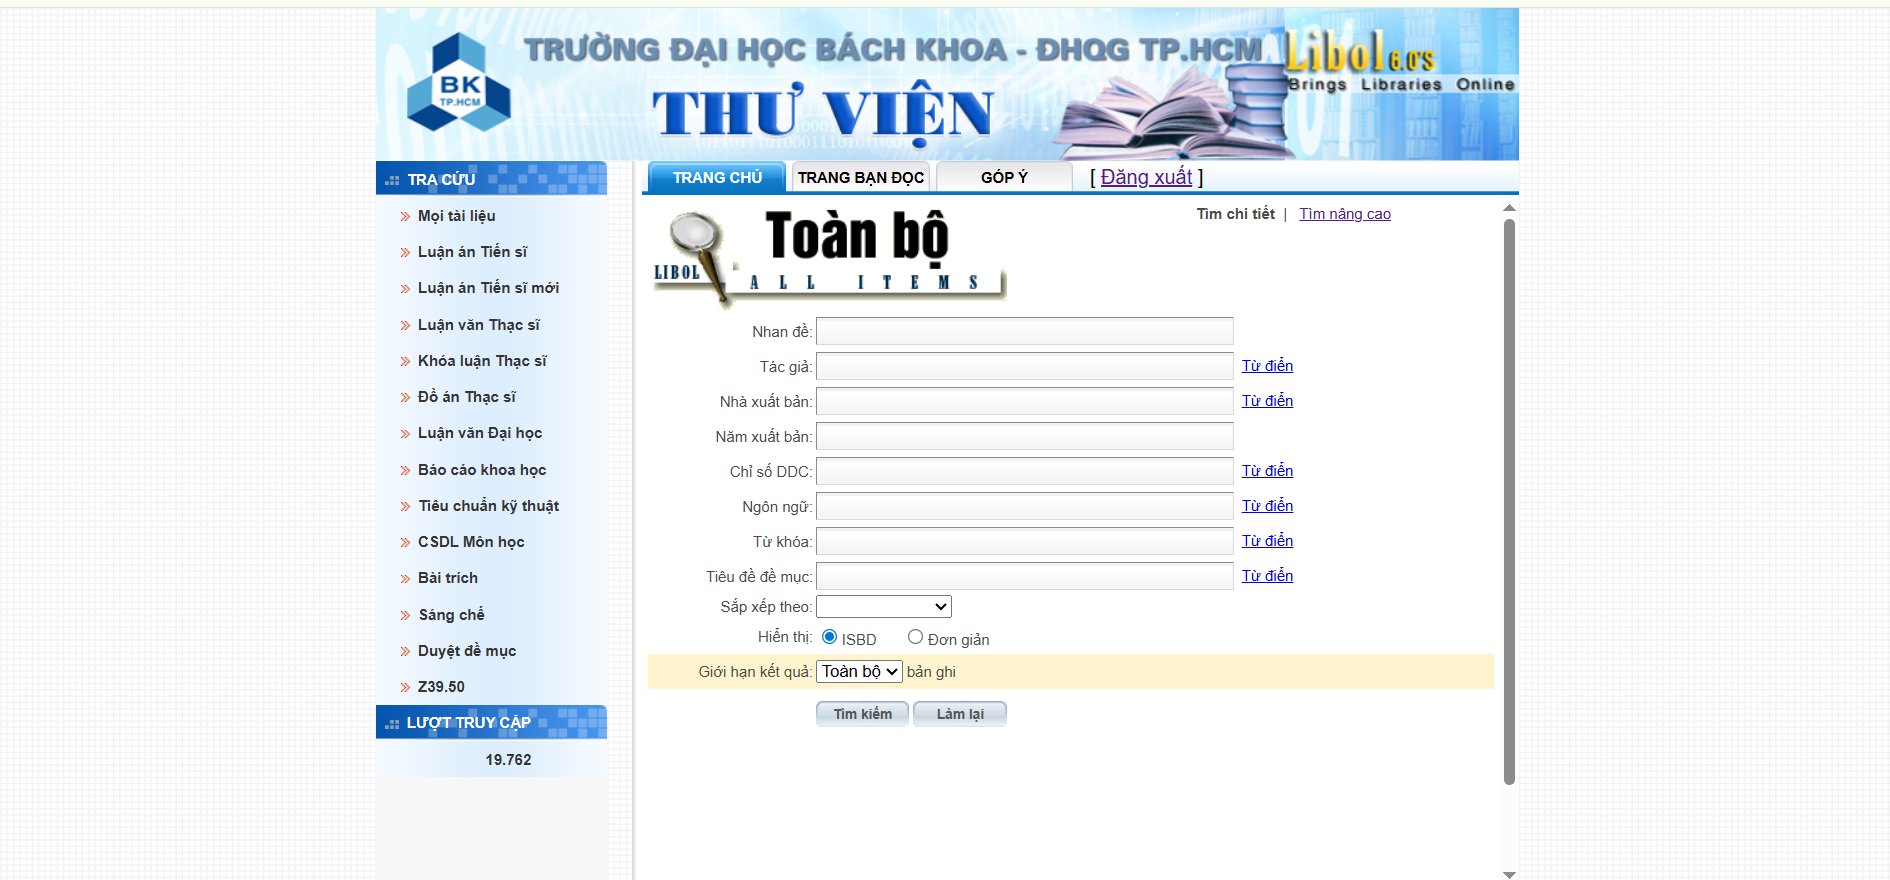
\includegraphics[width=0.8\linewidth]{Images/opac.lib.hcmut.edu.vn.png} 
     \vspace{10pt}
    \caption{Giao diện Tra cứu Tài liệu Lưu trữ Nội bộ và Mô-đun Đăng nhập Tài khoản trên cổng OPAC}
    \label{fig:opac_hcmut_search}
\end{figure}

Mặc dù cả hai cổng đều đáp ứng các nhu cầu vận hành cốt lõi, việc phân mảnh dữ liệu giữa tài liệu in và kho tài liệu số/lưu trữ nội bộ tạo ra sự bất tiện trong trải nghiệm của sinh viên. Hạn chế này là động lực để nhóm chúng tôi xây dựng một hệ thống quản lý thư viện hiện đại giúp hợp nhất dữ liệu tài nguyên và tối ưu hóa quy trình vận hành thông qua các giải pháp phần mềm hiện đại.

\subsubsection{Ưu điểm}
\begin{itemize}
    \item Giao diện chuyên biệt cho tài liệu lưu trữ nội bộ được tối ưu hóa để truy vấn các trường dữ liệu tả học thuật.
    \item Quy trình mượn-trả trực tuyến và đặt giữ chỗ hoàn toàn tương thích với các chính sách thư viện thực tế.
    \item Cơ chế xác thực Đăng nhập Một lần (SSO) đồng bộ tài khoản độc giả đồng thời bảo mật tài nguyên số.
\end{itemize}

\subsubsection{Hạn chế}
\begin{itemize}
    \item Việc duy trì hai cổng độc lập buộc độc giả phải thực hiện các thao tác tìm kiếm lặp đi lặp lại trên các tên miền riêng biệt.
    \item Cơ chế tìm kiếm dựa hoàn toàn vào khớp từ khóa chính xác, khả năng hiểu ngôn ngữ tự nhiên còn hạn chế.
    \item Kiến trúc nền tảng tĩnh thiếu các tính năng gợi ý tự động và công cụ trợ lý ảo AI 24/7.
    \item Giao diện tìm kiếm nâng cao chưa được tối ưu tốt cho các thiết bị di động, quy trình tương tác còn mang tính thủ tục.
\end{itemize}

\subsection{Hệ thống Thư viện Trực tuyến -- Đại học London (The Online Library -- UoL)}

Hệ thống Thư viện Trực tuyến của Đại học London (UoL) tại \url{https://onlinelibrary.london.ac.uk/} đại diện cho mô hình thư viện số (E-library) hàng đầu được thiết kế chuyên biệt để hỗ trợ sinh viên học từ xa trên toàn cầu. Khác với các mô hình quản lý bộ sưu tập vật lý truyền thống, hệ thống này vận hành hoàn toàn trên môi trường số, tập trung vào việc quản lý, lưu trữ và phân phối quyền truy cập vào các cơ sở dữ liệu học thuật, tạp chí điện tử (E-journals) và sách điện tử (E-books).

Điểm sáng kỹ thuật của hệ thống là việc triển khai Dịch vụ Khám phá Tập trung (Discovery Service). Thay vì yêu cầu người dùng đăng nhập vào từng nền tảng của nhà xuất bản, một thanh tìm kiếm hợp nhất (One-stop search) có thể truy vấn các mục toàn văn trên hàng trăm nguồn cơ sở dữ liệu. Hơn nữa, để bù đắp cho sự thiếu hụt hỗ trợ trực tiếp tại chỗ, hệ thống cung cấp công cụ hỗ trợ trực tuyến ("Chat với chúng tôi") hoạt động như một bàn trợ giúp 24/7 để giải quyết các thắc mắc kỹ thuật và hướng dẫn sinh viên tìm kiếm tài liệu.

\begin{figure}[H]
    \centering
     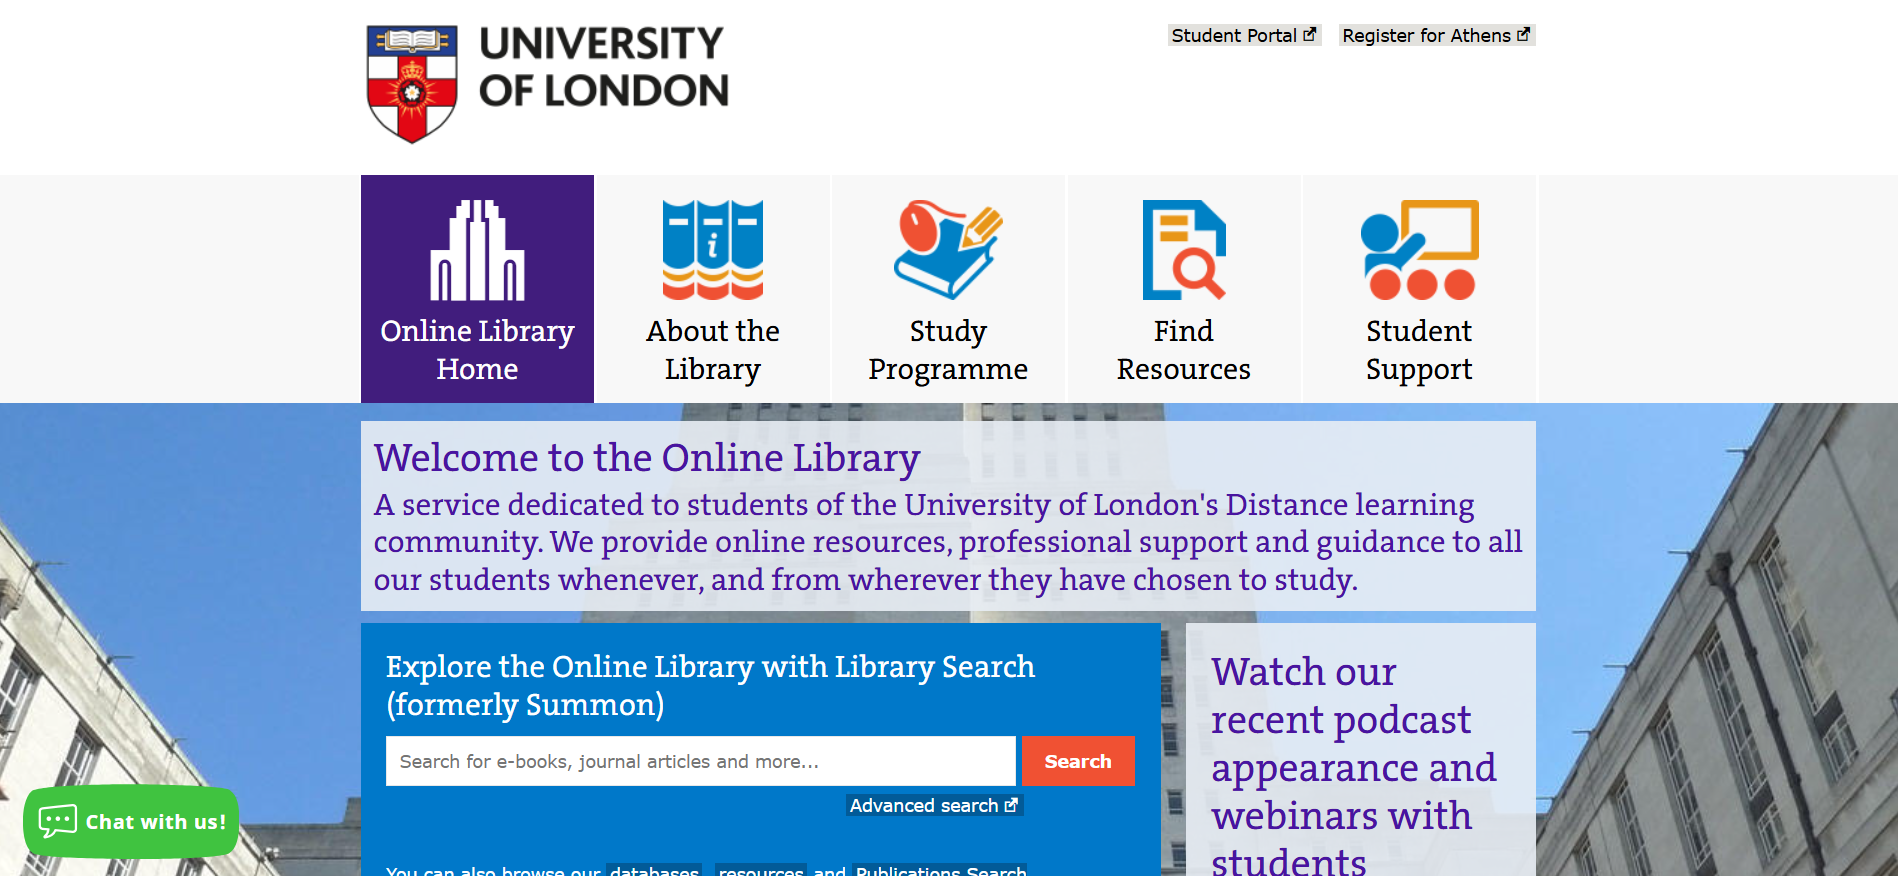
\includegraphics[width=0.8\linewidth]{Images/london_online_library_homepage.png} 
    \vspace{10pt}
    \caption{Giao diện tìm kiếm khám phá hợp nhất và công cụ hỗ trợ trực tuyến tại Thư viện Trực tuyến UoL}
    \label{fig:london_lib_homepage}
\end{figure}

Phân tích hệ thống của UoL mang lại những góc nhìn quan trọng về việc tối ưu hóa trải nghiệm người dùng số, đồng thời làm nổi bật các khoảng trống công nghệ trong việc tương tác thông minh với người dùng.

\subsubsection{Ưu điểm}
\begin{itemize}
    \item Cung cấp một cổng truy cập duy nhất cho tất cả các tài nguyên số, giảm thời gian tìm kiếm cho người dùng.
    \item Sử dụng các giao thức xác thực hiện đại (OpenAthens), cho phép truy cập từ xa ngoài khuôn viên trường một cách mượt mà mà không cần VPN.
    \item Phân loại tài liệu số theo các ngành học cụ thể để hướng dẫn sinh viên khám phá tài liệu hiệu quả.
\end{itemize}

\subsubsection{Hạn chế}
\begin{itemize}
    \item Mô hình chỉ giới hạn trong các tài sản số, bỏ qua hoàn toàn quy trình lưu thông sách vật lý và quản lý kho sách.
    \item Việc tìm kiếm khám phá tập trung có thể gây ra tình trạng quá tải thông tin và thiếu phân tích hành vi để gợi ý cá nhân hóa.
    \item Hỗ trợ chatbot hoạt động dựa trên các quy tắc kịch bản tĩnh, chưa thể hiểu các câu truy vấn phức tạp và phụ thuộc nhiều vào sự can thiệp của thủ thư.
\end{itemize}

\subsection{Hệ thống Thư viện Đại học Delaware (UD Library)}

Hệ thống Thư viện Đại học Delaware (UD Library) tại \url{https://library.udel.edu/} là minh họa cho mô hình quản trị thư viện đại học đa chi nhánh được số hóa cao. Khác với định hướng thuần số của UoL, UD Library giải quyết một bài toán phức tạp hơn: quản lý và phân phối dữ liệu giữa thư viện trung tâm và các thư viện khoa, đồng thời tiên phong tích hợp trợ lý ảo AI vào quy trình hỗ trợ sinh viên.

Cốt lõi của hệ thống này là \textbf{DELCAT} (Dịch vụ Khám phá Hợp nhất), đóng vai trò là giao diện duy nhất kết nối người dùng với hàng triệu bản ghi thuộc nhiều định dạng khác nhau. Đáng chú ý, UD Library đã bắt đầu triển khai các giải pháp AI giao tiếp bằng ngôn ngữ tự nhiên bên cạnh các cơ chế tìm kiếm truyền thống.

\begin{figure}[H]
\centering
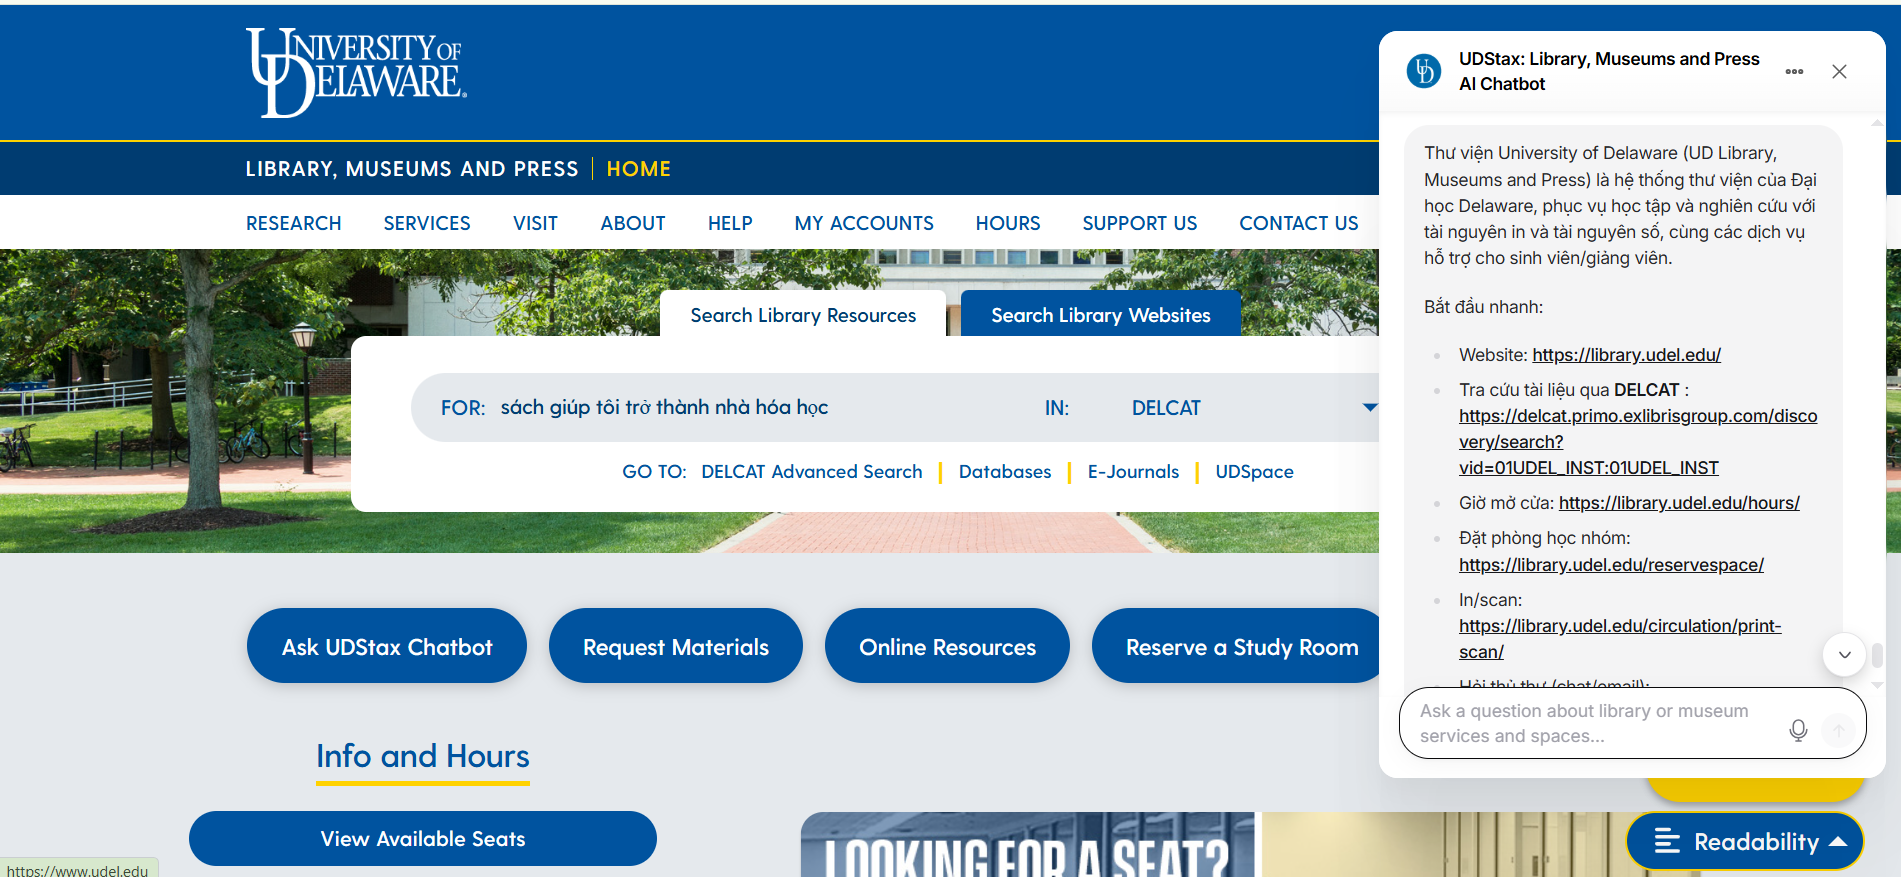
\includegraphics[width=0.8\linewidth]{Images/ud_library_homepage_chatbot.png} 
\vspace{10pt}
\caption{Giao diện dịch vụ khám phá hợp nhất DELCAT và công cụ AI hỗ trợ tại Thư viện UD}
\label{fig:ud_delcat_search}
\end{figure}

Tìm hiểu UD Library mang lại các góc nhìn kiến trúc quan trọng về việc xây dựng một nền tảng khám phá hợp nhất "Tất cả trong một" và vận hành các trợ lý AI giao tiếp trong môi trường học thuật lớn.

\subsubsection{Ưu điểm}
\begin{itemize}
\item Tích hợp các trợ lý ảo có khả năng xử lý ngôn ngữ tự nhiên để tự động hóa các câu hỏi Q\&A thủ tục thường gặp.
\item Nền tảng DELCAT hợp nhất việc khám phá sách in và tài nguyên điện tử trong một giao diện người dùng duy nhất.
\item Kết nối các dịch vụ thư viện phi truyền thống, như đặt phòng học nhóm, dịch vụ in ấn và mượn liên thư viện.
\end{itemize}

\subsubsection{Hạn chế}
\begin{itemize}
\item Chatbot hoạt động độc lập như một kênh tư vấn thủ tục mà chưa tích hợp sâu vào động cơ tìm kiếm để gợi ý sách trực tiếp.
\item Kiến trúc khám phá hợp nhất thường xuyên gây quá tải thông tin bằng cách trả về lượng kết quả tìm kiếm quá lớn.
\end{itemize}

\subsection{Hệ thống Quản lý Thư viện Mã nguồn Mở -- Koha ILS}

Koha ILS là Hệ thống Thư viện Tích hợp (ILS) mã nguồn mở được áp dụng rộng rãi nhất trên thế giới, được sử dụng bởi nhiều định chế giáo dục và mạng lưới thư viện công cộng. Khác với các cổng OPAC dành cho người dùng hoặc các nền tảng Khám phá được phân tích ở trên, Koha đại diện cho một hệ thống lõi backend tập trung vào việc số hóa và tự động hóa các quy trình quản lý hành chính phức tạp cho nhân viên thư viện (Thủ thư).

Thông qua cổng quản trị Staff Client, Koha cung cấp các mô-đun toàn diện để quản lý thư viện vật lý và thư viện số, bao gồm: Lưu thông, Biên mục Quốc tế, Quản lý Độc giả và Báo cáo Thống kê. Việc nghiên cứu Koha cung cấp các tiêu chuẩn tham chiếu giá trị cho việc thiết kế lược đồ cơ sở dữ liệu và logic quy tắc nghiệp vụ trong đồ án của chúng tôi.

\begin{figure}[H]
\centering
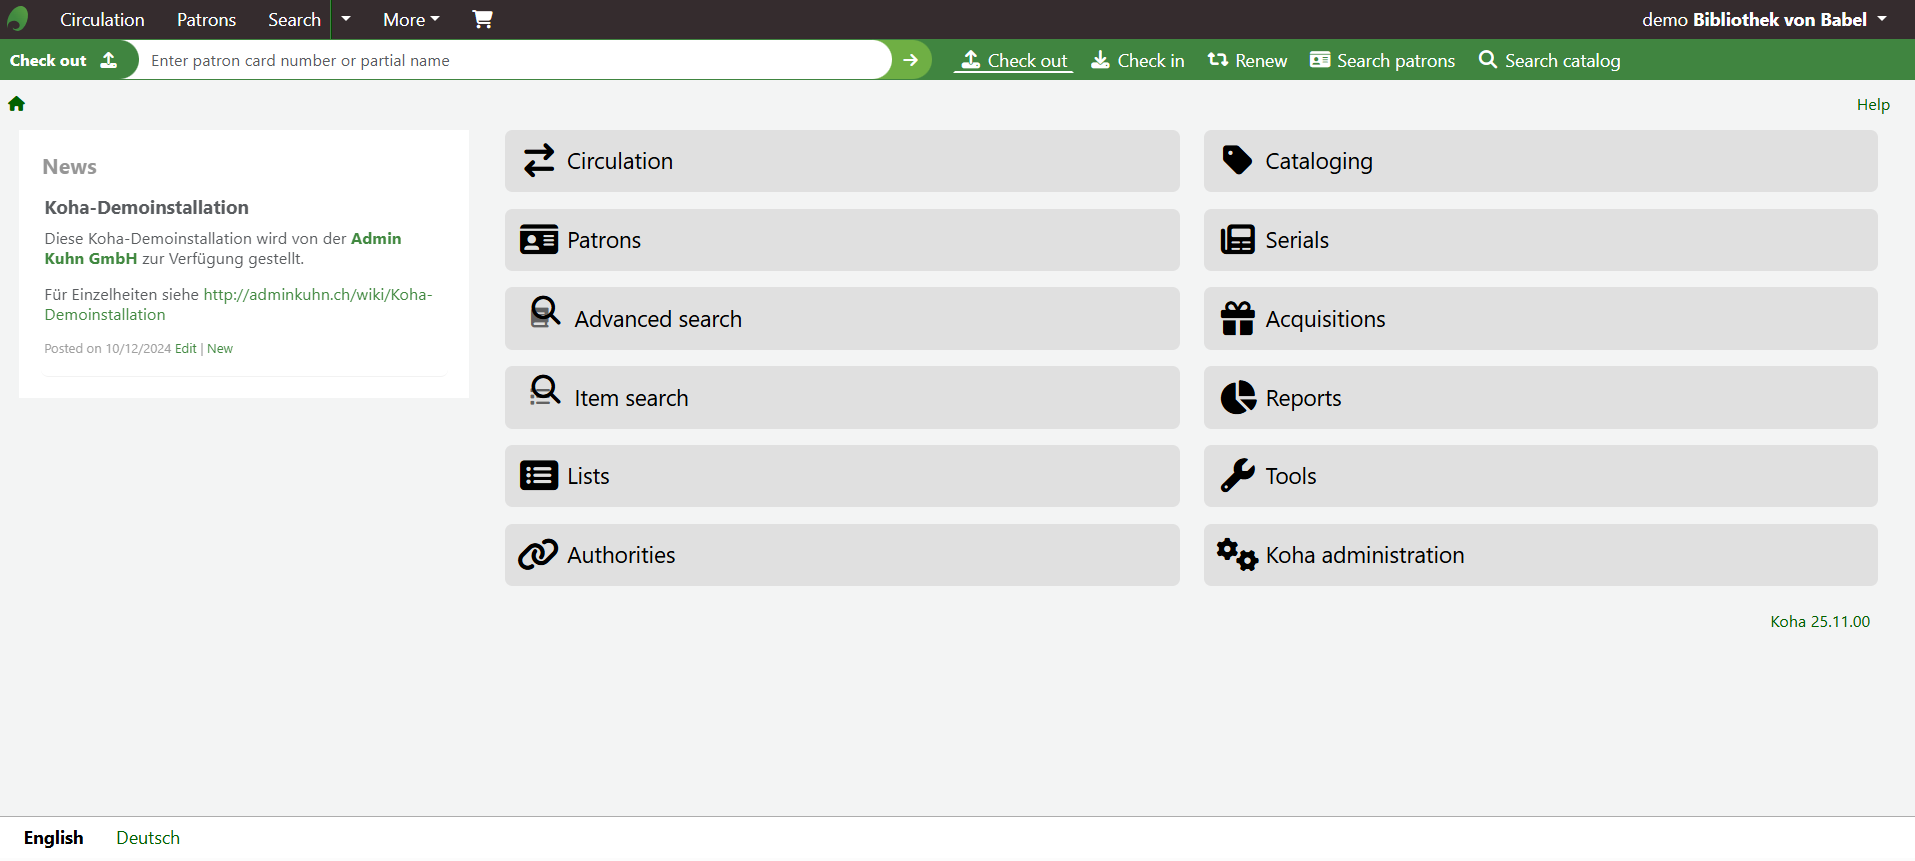
\includegraphics[width=0.8\linewidth]{Images/koha_staff_interface.png} 
\vspace{10pt}
\caption{Mô-đun giao diện quản trị Staff Client của Koha}
\label{fig:koha_admin}
\end{figure}

Phân tích Koha giúp xác định rõ các tính năng cốt lõi cần thiết trong một phần mềm quản lý thư viện, đồng thời chỉ ra các điểm bất tiện trong trải nghiệm người dùng hiện diện ở các hệ thống quản trị truyền thống.

\subsubsection{Ưu điểm}
\begin{itemize}
\item Tuân thủ nghiêm ngặt các tiêu chuẩn dữ liệu tả thư viện quốc tế (MARC21, Z39.50), đảm bảo tính nhất quán và khả năng tương thao dữ liệu.
\item Mô-đun lưu thông cung cấp ma trận quy tắc chi tiết để cấu hình logic mượn, trả, gia hạn và phạt quá hạn phù hợp với từng nhóm người dùng.
\item Tích hợp sẵn các REST API cho phép các ứng dụng bên thứ ba tương tác và trích xuất dữ liệu để mở rộng nền tảng.
\item Hệ thống báo cáo hỗ trợ các truy vấn SQL tùy chỉnh trực tiếp, mang lại sự linh hoạt tối đa cho các báo cáo quản trị.
\end{itemize}

\subsubsection{Hạn chế}
\begin{itemize}
\item Giao diện Staff Client (UI/UX) phức tạp, tuân theo các bố cục nhiều biểu mẫu truyền thống làm tăng thời gian đào tạo thủ thư.
\item Quy trình biên mục dữ liệu vẫn phụ thuộc nặng nề vào thao tác thủ công, thiếu các cơ chế phân loại tự động thông minh hoặc trích xuất dữ liệu tả.
\item Kiến trúc hệ thống đơn khối (monolithic) và lược đồ cơ sở dữ liệu quan hệ phức tạp cản trở việc tách biệt nhanh chóng hoặc bổ sung các tính năng mô-đun tùy chỉnh.
\end{itemize}
\newpage
% % \section{Technology Stack}
% \subsection{Front-end: React.js and Vite}
% React.js handles the presentation layer of the online library, constructing interactive interfaces for book search, catalog browsing, and AI assistant chat interactions. Vite is employed as the build tool and dev server to provide fast startup, HMR support, and optimized production bundle compilation. On the client side, components handle rendering search results (incorporating keyword highlights and semantic matches), managing user state (caching, optimistic updates), and integrating the AI chat/assistant SDK (streaming responses, conversation state).
% \begin{figure}[htbp]
%     \centering
%     
\includegraphics[width=0.4\textwidth]{Images/react_vite.png}
% \end{figure}

% \subsection{Back-end: Node.js and Express}
% Node.js + Express provides the core REST API for book catalog management, user accounts, and session administration. The server orchestrates request routing, authentication, RBAC authorization, PostgreSQL transactions via Prisma, and delegates AI workloads (embedding generation, summarization, RAG queries) to dedicated AI services. It exposes standardized endpoints for search, recommendations, and integration webhooks (e.g., metadata enrichment from Open Library).
% \begin{figure}[htbp]
%     \centering
%     
\includegraphics[width=0.4\textwidth]{Images/node_express.jpg}
% \end{figure}

% \subsection{Dedicated AI Microservice: Python and FastAPI}
% A decoupled microservice implemented in Python + FastAPI leverages NLP and Machine Learning frameworks (transformers, sentence-transformers, LLM provider client SDKs). Its primary responsibilities include embedding vector generation, document summarization, RAG-based question answering, and prompt engineering pipelines (chunking, reranking). FastAPI is ideal for low-latency concurrent endpoints and seamlessly scales based on workload demands.
% \begin{figure}[htbp]
%     \centering
%     
\includegraphics[width=0.4\textwidth]{Images/fastapi.png}
% \end{figure}

% \subsection{ORM: Prisma}
% Prisma (TypeScript) is used to define database schemas, generate type-safe query clients, and manage PostgreSQL migrations. Prisma maintains end-to-end type safety between the Node application and the database layer, simplifying queries related to loans, transaction logs, and catalog metadata while providing ACID transaction support for data consistency.
% \begin{figure}[htbp]
%     \centering
%     
\includegraphics[width=0.4\textwidth]{Images/prisma.png}
% \end{figure}

% \subsection{Relational Database: PostgreSQL}
% PostgreSQL serves as the primary relational store for book records, user profiles, loan transactions, and system metadata. Key advantages include strict ACID compliance for loan-return workflows, advanced JSONB support for flexible metadata, full-text keyword indexing, and horizontal scalability via replication and partitioning.
% \begin{figure}[htbp]
%     \centering
%     
\includegraphics[width=0.4\textwidth]{Images/postgresql.jpg}
% \end{figure}

% \subsection{Vector Store and Embeddings: pgvector}
% Text embeddings for book contents (full texts, summaries) are stored in `pgvector` (a vector extension for PostgreSQL) or a dedicated vector database. The vector store performs nearest-neighbor searches (cosine similarity) to power semantic search, contextual retrieval for RAG pipelines, and "similar books" recommendation features, mapping vector outputs directly to source document IDs.

% \subsection{AI / LLM Capabilities: Embeddings, RAG, Summarization, and Chatbot}
% The system integrates Large Language Models (LLMs) across multiple modules: embedding generation for semantic search, Retrieval-Augmented Generation (RAG) for Q\&A based on library documents, automatic chapter/abstract summarization for previews, and interactive chatbot assistants. The architecture incorporates controlled prompt templates, embedding caching, and attribution mechanisms for source citation.
% \begin{figure}[htbp]
%     \centering
%     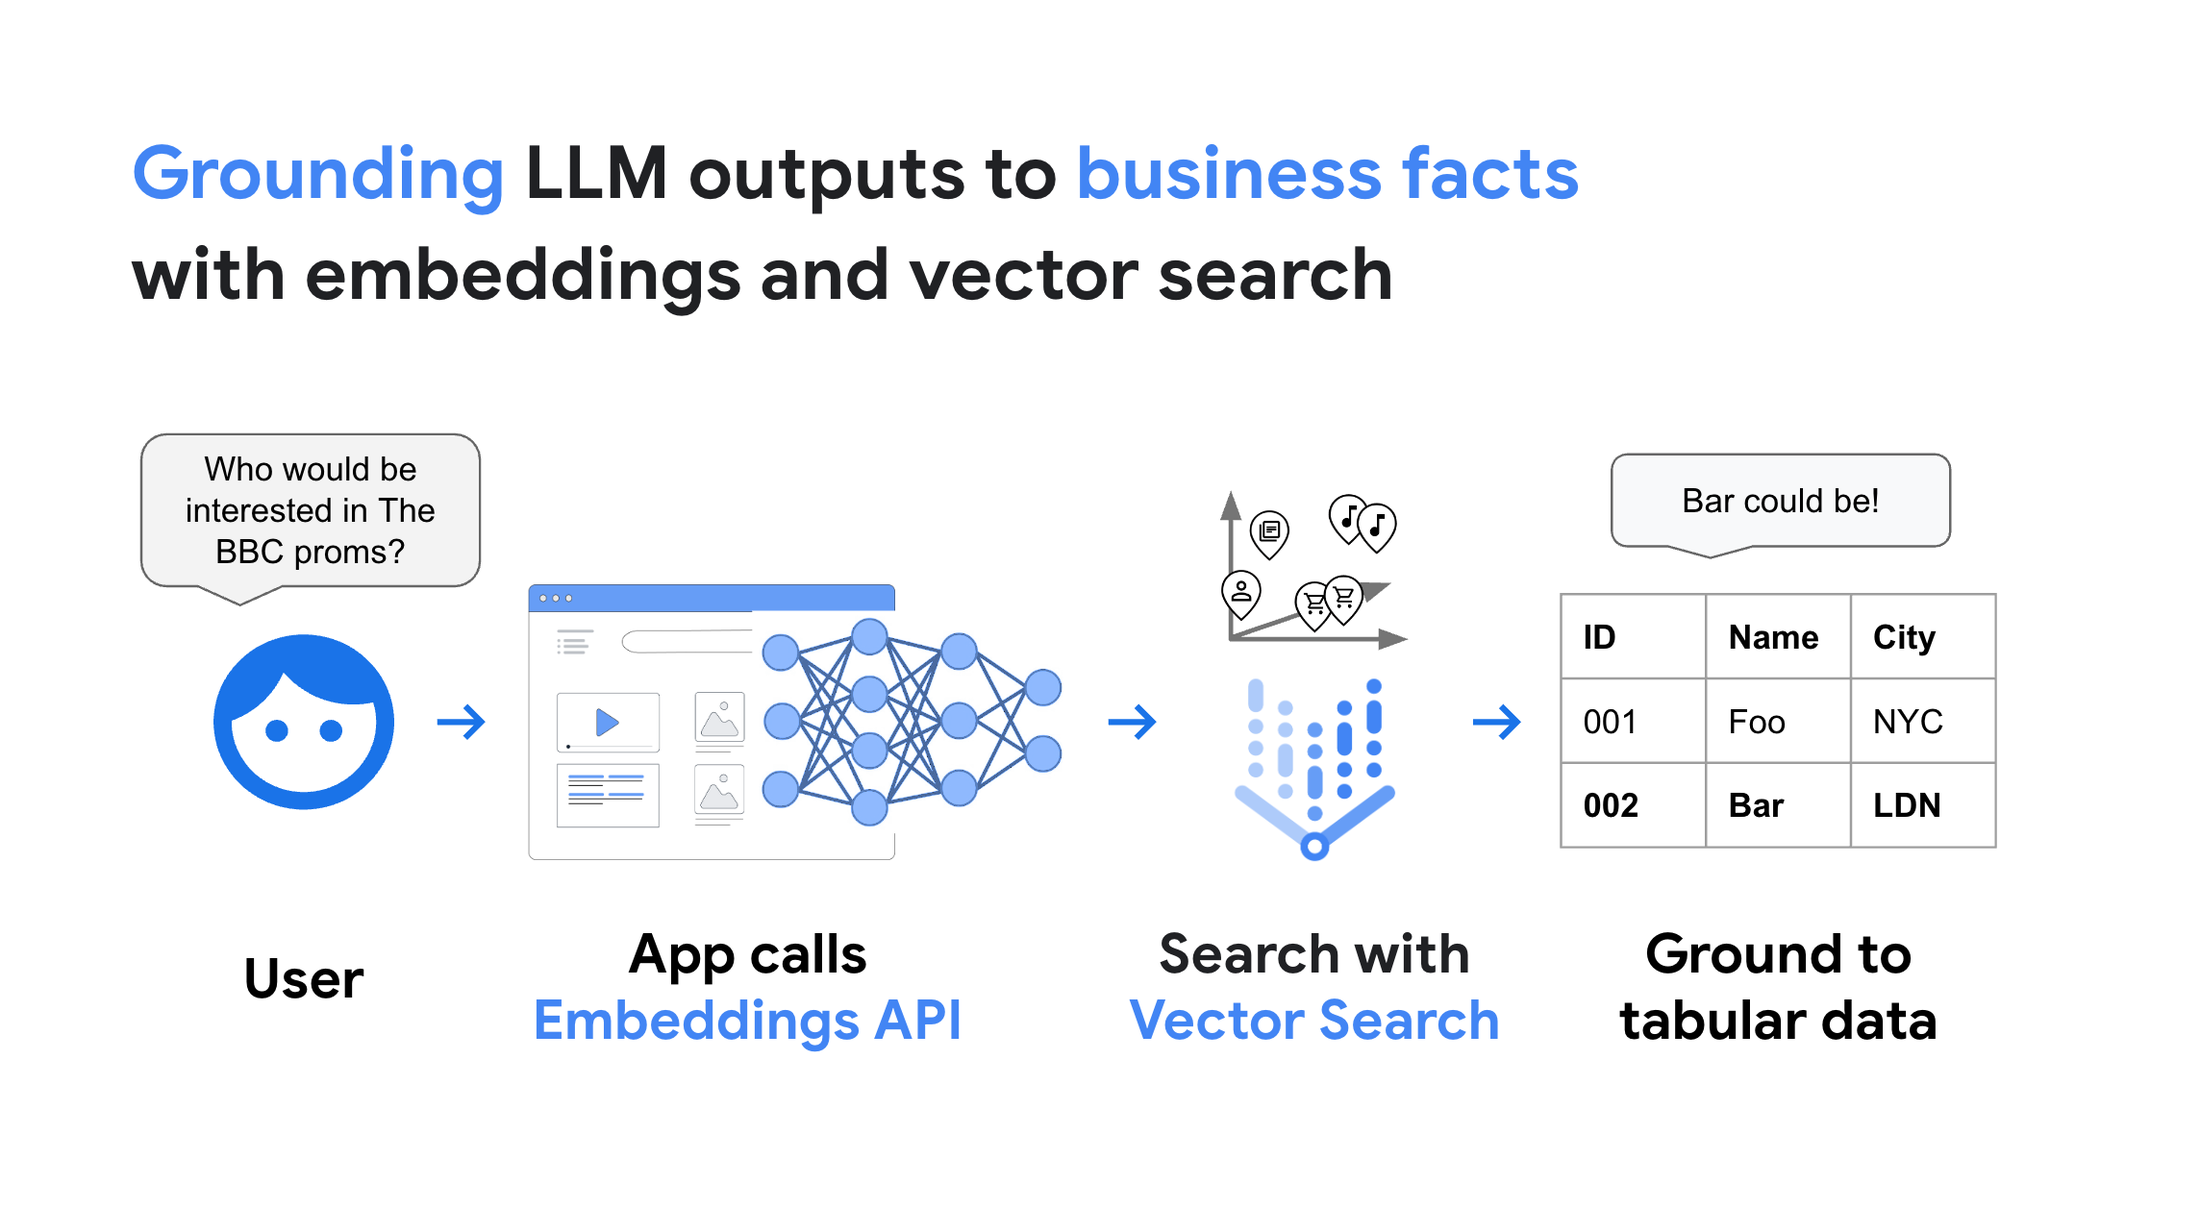
\includegraphics[width=0.5\textwidth]{Images/EmbeddingsAPI.png}
% \end{figure}

% \subsection{Hybrid Search Strategy}
% A hybrid search strategy combines: 1) full-text keyword search on PostgreSQL for exact metadata matching; and 2) vector similarity search via pgvector for semantic retrieval and contextual matching. Results are merged and reranked (based on relevance scores, popularity, and user context) before returning to the client interface.

% \subsection{Security and Authentication: JWT, RBAC, and OTP}
% The system utilizes JSON Web Tokens (JWT) for session management and refresh tokens for secure persistence. Role-Based Access Control (RBAC) enforces granular permissions (Admin, Librarian, Reader) verified at API gateways and endpoints. One-Time Passwords (OTP via email/SMS) secure multi-factor authentication for sensitive operations. Additional measures include HTTPS/TLS encryption, rate limiting, and comprehensive audit logging.

% \subsection{External Integrations: Open Library, Google Books, and Nodemailer}
% The Open Library and Google Books APIs automate metadata, cover image, and publishing data fetching via ISBN lookup. An automated ETL pipeline periodically syncs catalog data. `Nodemailer` handles transactional notifications (loan due reminders, password resets, system alerts) with dynamic HTML templates and delivery logging.
% \begin{figure}[htbp]
%     \centering
%     
\includegraphics[width=0.3\textwidth]{Images/Google-play-book-icon.png}
% \end{figure}
% \newpage
\section{Yêu cầu Hệ thống}
\subsection{Yêu cầu Chức năng}
\subsubsection{Quản lý Tài khoản Người dùng}
- Hệ thống phải cho phép người dùng mới (độc giả) đăng ký tài khoản bằng cách cung cấp họ tên, địa chỉ email, mã số sinh viên/mã nhân viên và mật khẩu. \\
- Hệ thống phải xác thực người dùng qua tên đăng nhập/email và mật khẩu. Hỗ trợ tùy chọn Xác thực Nhiều yếu tố (MFA) cho các tài khoản quản trị viên. \\
- Hệ thống phải hỗ trợ ít nhất ba vai trò người dùng: Độc giả, Thủ thư và Quản trị viên, mỗi vai trò được gán các quyền hạn riêng biệt.\\
- Người dùng phải có khả năng xem và cập nhật thông tin hồ sơ cá nhân, bao gồm chi tiết liên hệ và tùy chọn thông báo.\\
- Hệ thống phải cho phép người dùng đặt lại mật khẩu thông qua các liên kết xác thực gửi đến địa chỉ email đã đăng ký.\\
- Quản trị viên phải có quyền kích hoạt, vô hiệu hóa hoặc tạm khóa bất kỳ tài khoản người dùng nào.\\
- Hệ thống phải ghi lại lịch sử mượn trả của từng độc giả, cho phép độc giả đó và các thủ thư có thẩm quyền truy cập xem.\\

\subsubsection{Quản lý Danh mục Tài nguyên}
- Hệ thống phải duy trì danh mục tất cả tài sản thư viện, bao gồm sách in và ấn phẩm định kỳ.\\
- Mỗi bản ghi danh mục phải lưu trữ: tên sách, tác giả, ISBN/ISSN, nhà xuất bản, năm xuất bản, lần xuất bản, thể loại/chủ đề, ngôn ngữ, vị trí vật lý (mã kệ/phân loại), tổng số bản sao và số bản sao khả dụng.\\
- Thủ thư phải có khả năng thêm, sửa, xóa các bản ghi danh mục thông qua giao diện quản trị.\\
- Hệ thống phải hỗ trợ nhập dữ liệu danh mục hàng loạt qua các định dạng tệp CSV hoặc MARC21.\\
- Hệ thống phải cung cấp khả năng tìm kiếm toàn văn trên các trường tên sách, tác giả, ISBN, chủ đề và từ khóa.\\
- Kết quả tìm kiếm phải hỗ trợ lọc theo thể loại, ngôn ngữ, trạng thái khả dụng, khoảng năm xuất bản và định dạng tư liệu.\\
- Hệ thống phải hiển thị tình trạng khả dụng thực tế của từng mục theo thời gian thực, bao gồm số lượng khả dụng, đang mượn và đang đặt giữ chỗ.\\

\subsubsection{Quản lý Lưu thông Tài liệu}
- Hệ thống phải cho phép độc giả mượn tài liệu vật lý bằng cách quét mã vạch hoặc nhập thủ công tại bàn lưu thông, hoặc gửi yêu cầu đặt lấy sách trực tuyến.\\
- Hệ thống phải áp dụng hạn mức mượn dựa trên vai trò người dùng (ví dụ: tối đa 5 tài liệu cho sinh viên, tối đa 15 tài liệu cho giảng viên).\\
- Hệ thống phải gán hạn trả cho các tài liệu mượn dựa trên các quy tắc thời hạn mượn có thể cấu hình theo từng loại tư liệu.\\
- Hệ thống phải cho phép độc giả gia hạn các tài liệu đang mượn trực tuyến lên đến số lần tối đa được cấu hình, với điều kiện không có yêu cầu đặt chỗ nào khác cho các tài liệu đó.\\
- Hệ thống phải cho phép độc giả đặt mượn trước (hold) đối với các tài liệu hiện đang được mượn bởi người dùng khác.\\
- Hệ thống phải tự động thông báo cho người dùng tiếp theo trong hàng chờ đặt chỗ khi tài liệu được trả về trạng thái khả dụng.\\
- Hệ thống phải xử lý việc trả tài liệu và ngay lập tức cập nhật lại số lượng bản sao khả dụng trong danh mục.\\
- Hệ thống phải tự động tính tiền phạt quá hạn dựa trên mức phí hằng ngày có thể cấu hình theo từng loại tài liệu.\\
- Hệ thống phải cho phép độc giả xem các khoản mượn hiện tại, hạn trả, lượt đặt chỗ và tiền phạt chưa thanh toán từ bảng điều khiển cá nhân.\\
- Hệ thống phải hỗ trợ mượn liên chi nhánh, cho phép độc giả yêu cầu tài liệu từ các thư viện chi nhánh khác trong cùng mạng lưới.\\

\subsubsection{Động cơ Gợi ý Tài liệu bằng AI}
- Hệ thống phải tạo các gợi ý sách và tài nguyên được cá nhân hóa cho độc giả dựa trên lịch sử mượn, nhật ký tìm kiếm và các mục được đánh giá.\\
- Động cơ gợi ý phải kết hợp lọc cộng tác (phân tích sở thích của các người dùng tương tự) và lọc dựa trên nội dung (phân tích các thuộc tính dữ liệu tả của mục).\\

\subsubsection{Tìm kiếm Ngôn ngữ Tự nhiên AI và Tương tác Thông minh}
- Hệ thống phải cung cấp giao diện tìm kiếm bằng ngôn ngữ tự nhiên cho phép độc giả truy vấn danh mục bằng các diễn đạt dạng giao tiếp.\\
- Mô-đun tìm kiếm ngôn ngữ tự nhiên phải phân tích ý định của người dùng, trích xuất các thuộc tính (thể loại, đối tượng hướng tới, chủ đề, độ dài) và ánh xạ chúng với dữ liệu tả danh mục.\\
- Hệ thống phải hiển thị kết quả tìm kiếm ngôn ngữ tự nhiên được xếp hạng theo độ liên quan bên cạnh các kết quả tìm kiếm từ khóa tiêu chuẩn.\\
- Hệ thống phải tích hợp Chatbot Trợ lý ảo để tương tác trực tiếp với người dùng, giải đáp các thắc mắc Q\&A về quy định thư viện, giờ mở cửa và quy trình mượn sách.\\

\subsubsection{Biên mục và Tóm tắt Hỗ trợ bởi AI}
- Tự động điền dữ liệu tả sách (Tên sách, Tác giả, Mô tả) khi thủ thư nhập mã ISBN.\\
- AI tự động tạo bản tóm tắt ngắn gọn cho các sách mới được biên mục để độc giả xem trước.\\

\subsubsection{Thông báo và Tương tác}
- Hệ thống phải gửi các thông báo tự động qua email/SMS cho: nhắc nhở trước hạn 3 ngày, cảnh báo quá hạn, thông báo sách đặt chỗ đã sẵn sàng và cập nhật trạng thái tài khoản.\\
- Độc giả phải có khả năng cấu hình kênh thông báo và tần suất nhận trong phần cài đặt hồ sơ.\\
- Hệ thống phải cung cấp một trung tâm thông báo trong ứng dụng hiển thị các cảnh báo chưa đọc.\\
- Thủ thư phải có khả năng phát các thông báo đại chúng (như thông báo đóng cửa thư viện) đến tất cả người dùng hoặc các nhóm đối tượng cụ thể.\\

\subsubsection{Báo cáo và Phân tích}
- Hệ thống phải tạo các báo cáo phân tích về: các mục được mượn nhiều nhất, tài liệu quá hạn, tổng hợp thu tiền phạt, đăng ký người dùng mới và chỉ số phát triển danh mục.\\
- Hệ thống phải cung cấp bảng điều khiển theo thời gian thực cho thủ thư hiển thị các chỉ số vận hành chính: lượt mượn đang hoạt động, số lượng quá hạn, số lượng khả dụng và khối lượng giao dịch hằng ngày.\\
- Báo cáo phải hỗ trợ xuất ra các định dạng PDF và Excel.\\

\subsubsection{Quản trị và Cấu hình Hệ thống}
- Quản trị viên phải có khả năng cấu hình các tham số toàn cục bao gồm thời hạn mượn, mức phí phạt, hạn mức mượn theo vai trò và ngưỡng hết hạn đặt chỗ.\\
- Hệ thống phải hỗ trợ quản lý thư viện đa chi nhánh.\\
- Hệ thống phải ghi nhật ký kiểm toán (audit log) đầy đủ cho các hành động quản trị (thay đổi cấu hình, chỉnh sửa tài khoản, nhập dữ liệu hàng loạt).\\

\subsection{Yêu cầu Phi Chức năng}

Để đảm bảo vận hành ổn định, bảo mật và trải nghiệm người dùng mượt mà, hệ thống tuân thủ các tiêu chuẩn phi chức năng sau:

\begin{itemize}
    \item \textbf{Thời gian Tải Trang:} Trang chủ, trang tìm kiếm tài liệu và trang chi tiết sách phải hoàn tất tải trong dưới 3 giây (tối ưu hóa đạt 1.5 giây) trên cả nền tảng máy tính và di động.
    
    \item \textbf{Thời gian Phản hồi API:} 
    \begin{itemize}
        \item Các API nghiệp vụ cơ bản (kiểm tra giỏ mượn, lịch sử mượn) phải phản hồi trong vòng 0.5 giây.
        \item Các API xử lý thông minh (Trợ lý ảo AI, tóm tắt văn bản, tìm kiếm ngữ nghĩa) phải trả về kết quả trong vòng 3 giây.
    \end{itemize}
    
    \item \textbf{Khả năng Chịu tải:} Hệ thống phải xử lý ổn định từ 1.000 đến 2.000 phiên làm việc của độc giả đồng thời mà không suy giảm hiệu năng máy chủ.
    
    \item \textbf{Tính Nhất quán UI/UX:} Kiểu chữ, bảng màu thương hiệu, bố cục điều hướng và các nút hành động (Gia hạn, Đặt chỗ, Xử lý) phải duy trì nhất quán trên tất cả các màn hình.
    
    \item \textbf{Bảo mật Dữ liệu \& Quyền Riêng tư:} 
    \begin{itemize}
        \item Mật khẩu tài khoản người dùng phải được băm bằng các thuật toán mạnh (bcrypt) trước khi lưu vào cơ sở dữ liệu; nghiêm cấm việc ghi nhật ký mật khẩu dạng văn bản thuần.
        \item Truyền tải dữ liệu giữa máy khách và máy chủ phải được mã hóa qua các giao thức TLS/HTTPS.
    \end{itemize}
    
    \item \textbf{Bảo mật Ứng dụng:} Mã nguồn phải áp dụng tham số hóa nghiêm ngặt để ngăn chặn các lỗ hổng web bao gồm SQL Injection và Cross-Site Scripting (XSS).
    
    \item \textbf{Thời gian Hoạt động (Uptime):} Hạ tầng máy chủ phải duy trì thời gian hoạt động tối thiểu 99.5\% mỗi năm, không tính các khoảng thời gian bảo trì được hạ tầng lên lịch trước.
    
    \item \textbf{Khôi phục Sau Sự cố:} Sao lưu cơ sở dữ liệu được thực hiện hằng ngày. Trong các sự cố hỏng hóc phần cứng, thời gian khôi phục về trạng thái sao lưu mới nhất phải diễn ra trong vòng 4 giờ.
    
    \item \textbf{Khả năng Tích hợp:} Kiến trúc mô-đun sử dụng các REST API tiêu chuẩn giúp dễ dàng tích hợp với các dịch vụ bên ngoài (cổng thông tin nhà trường, Google Books API).
\end{itemize}

\newpage
\section{Đặc tả Chi tiết các Use-case}

% ======================================================================================
% 4.1 ACCOUNT AND ACCESS MANAGEMENT
% ======================================================================================
\subsection{Quản lý Tài khoản và Truy cập Người dùng}

\subsubsection{Tổng quan}

\begin{figure}[H]
    \centering
    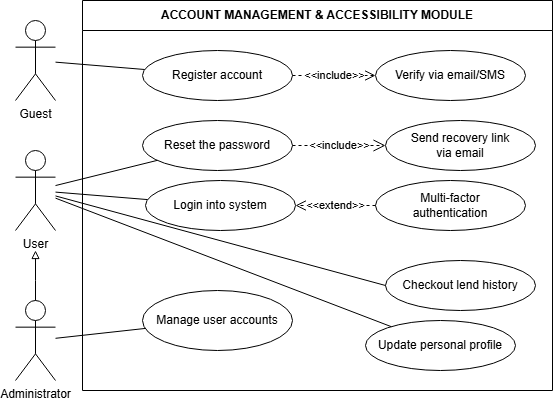
\includegraphics[width=0.8\linewidth]{Images/Quan_ly_tai_khoan_truy_cap.png}
    \vspace{10pt}
    \caption{Sơ đồ Use-case Quản lý Tài khoản và Truy cập Người dùng}
    \label{fig:usecase_account}
\end{figure}

\subsubsection{Đặc tả Chi tiết}

% --- UC: REGISTER ACCOUNT ---
\begin{longtable}{|p{3.5cm}|p{11.5cm}|}
    \hline
    \textbf{Tên Use-case} & \textbf{Đăng ký Tài khoản} \\
    \hline
    \textbf{Mã Use-case} & UC-ACC-01 \\
    \hline
    \textbf{Tổng quan} & Allows unregistered users to sign up and become system members. \\
    \hline
    \textbf{Tác nhân} & Khách \\
    \hline
    \textbf{Điều kiện tiên quyết} & Guest accesses the registration page of the system. \\
    \hline
    \textbf{Điều kiện kích hoạt} & Guest clicks the "Register" button. \\
    \hline
    \textbf{Luồng sự kiện} & 
    1. System displays the registration form.\newline
    2. Guest inputs required fields (Full name, Email, Password, etc.).\newline
    3. System validates input data integrity.\newline
    4. \textbf{[Bao gồm]} System executes "Send Verification Email/SMS" containing an OTP or activation link to the registered contact info.\newline
    5. Guest inputs the verification code or clicks the activation link.\newline
    6. System verifies the token, creates a new account, and persists it to the database.\newline
    7. System displays a success message. \\
    \hline
    \textbf{Điều kiện sau} & Account is created successfully and status transitions to "Activated". \\
    \hline
    \textbf{Ngoại lệ} & 
    Ex1: Email/Phone number already exists $\rightarrow$ System reports an error and requests re-entry.\newline
    Ex2: Invalid verification code entered beyond maximum attempts $\rightarrow$ Cancel registration session. \\
    \hline
    \caption{Đặc tả Use-case: Đăng ký Tài khoản}
\end{longtable}

\newpage
% --- UC: RESET PASSWORD ---
\begin{longtable}{|p{3.5cm}|p{11.5cm}|}
    \hline
    \textbf{Tên Use-case} & \textbf{Đặt lại Mật khẩu} \\
    \hline
    \textbf{Mã Use-case} & UC-ACC-02 \\
    \hline
    \textbf{Tổng quan} & Assists users in recovering account access when forgetting login passwords. \\
    \hline
    \textbf{Tác nhân} & Người dùng (Tất cả vai trò) \\
    \hline
    \textbf{Điều kiện tiên quyết} & User possesses an existing system account but cannot recall password. \\
    \hline
    \textbf{Điều kiện kích hoạt} & User clicks "Forgot Password" on the login view. \\
    \hline
    \textbf{Luồng sự kiện} & 
    1. System prompts user for registered email.\newline
    2. User inputs email and submits.\newline
    3. System verifies email existence in the database.\newline
    4. \textbf{[Bao gồm]} System triggers "Send Recovery Link via Email" flow.\newline
    5. User accesses the reset link received in email.\newline
    6. System renders password reset screen.\newline
    7. User inputs new password and confirms.\newline
    8. System hashes and updates new password, showing success alert. \\
    \hline
    \textbf{Điều kiện sau} & User password is updated successfully. \\
    \hline
    \textbf{Ngoại lệ} & 
    Ex1: Email does not exist $\rightarrow$ Display "No account found associated with this email".\newline
    Ex2: Reset link expired $\rightarrow$ Prompt user to restart the reset process. \\
    \hline
    \caption{Đặc tả Use-case: Đặt lại Mật khẩu}
\end{longtable}

% --- UC: USER LOGIN ---
\begin{longtable}{|p{3.5cm}|p{11.5cm}|}
    \hline
    \textbf{Tên Use-case} & \textbf{Đăng nhập Hệ thống} \\
    \hline
    \textbf{Mã Use-case} & UC-ACC-03 \\
    \hline
    \textbf{Tổng quan} & Authenticates user identity to grant system access matching role privileges. \\
    \hline
    \textbf{Tác nhân} & Người dùng (Tất cả vai trò) \\
    \hline
    \textbf{Điều kiện tiên quyết} & User possesses an active account in the system. \\
    \hline
    \textbf{Điều kiện kích hoạt} & User accesses the login view and enters credentials. \\
    \hline
    \textbf{Luồng sự kiện} & 
    1. User submits identity credentials (Email/Username) and Password.\newline
    2. System validates input formats and matches credentials against DB.\newline
    3. \textbf{[Mở rộng]} If Multi-Factor Authentication (MFA) is configured, system triggers "MFA Verification", requesting OTP from app/SMS.\newline
    4. Initializes user session (Session/JWT Token).\newline
    5. Redirects user to the dashboard corresponding to their assigned Role. \\
    \hline
    \textbf{Điều kiện sau} & User logs in successfully; system records login timestamp audit. \\
    \hline
    \textbf{Ngoại lệ} & 
    Ex1: Incorrect credentials $\rightarrow$ Display "Incorrect account or password".\newline
    Ex2: Account suspended $\rightarrow$ Display "Your account is locked. Please contact Admin".\newline
    Ex3: MFA code failed > 3 attempts $\rightarrow$ Lock login session temporarily for 15 minutes. \\
    \hline
    \caption{Đặc tả Use-case: Đăng nhập Hệ thống}
\end{longtable}

\newpage
% --- UC: UPDATE PROFILE ---
\begin{longtable}{|p{3.5cm}|p{11.5cm}|}
    \hline
    \textbf{Tên Use-case} & \textbf{Cập nhật Hồ sơ Người dùng} \\
    \hline
    \textbf{Mã Use-case} & UC-ACC-04 \\
    \hline
    \textbf{Tổng quan} & Allows users to modify personal profile information on the platform. \\
    \hline
    \textbf{Tác nhân} & Người dùng \\
    \hline
    \textbf{Điều kiện tiên quyết} & User is currently logged into the system. \\
    \hline
    \textbf{Điều kiện kích hoạt} & User accesses "Profile Settings" and selects "Edit". \\
    \hline
    \textbf{Luồng sự kiện} & 
    1. System populates form with current profile data.\newline
    2. User updates permissible fields (Phone, address, avatar image...).\newline
    3. User clicks "Save".\newline
    4. System validates field constraints.\newline
    5. Updates database record and displays success notification. \\
    \hline
    \textbf{Điều kiện sau} & User profile is updated. \\
    \hline
    \textbf{Ngoại lệ} & 
    Ex1: Invalid avatar format or file size exceeded $\rightarrow$ Warning alert and file rejection. \\
    \hline
    \caption{Đặc tả Use-case: Cập nhật Hồ sơ Người dùng}
\end{longtable}

% --- UC: VIEW BORROWING HISTORY ---
\begin{longtable}{|p{3.5cm}|p{11.5cm}|}
    \hline
    \textbf{Tên Use-case} & \textbf{Xem Lịch sử Mượn/Trả} \\
    \hline
    \textbf{Mã Use-case} & UC-ACC-05 \\
    \hline
    \textbf{Tổng quan} & Enables users to review past and active item borrowings along with their statuses. \\
    \hline
    \textbf{Tác nhân} & Người dùng \\
    \hline
    \textbf{Điều kiện tiên quyết} & User is logged into the system. \\
    \hline
    \textbf{Điều kiện kích hoạt} & User selects "Borrowing History" in personal dashboard. \\
    \hline
    \textbf{Luồng sự kiện} & 
    1. System receives user request.\newline
    2. Queries database for circulation records tied to user ID.\newline
    3. Renders loan list (Item title, borrow date, due date, return date, status, fines).\newline
    4. User can filter results by date range or status. \\
    \hline
    \textbf{Điều kiện sau} & System state remains unchanged. \\
    \hline
    \textbf{Ngoại lệ} & 
    Ex1: No loan records found $\rightarrow$ Display "You have no borrowing history". \\
    \hline
    \caption{Đặc tả Use-case: Xem Lịch sử Mượn/Trả}
\end{longtable}

\newpage
% --- UC: USER ACCOUNT MANAGEMENT (ADMIN) ---
\begin{longtable}{|p{3.5cm}|p{11.5cm}|}
    \hline
    \textbf{Tên Use-case} & \textbf{Quản lý Tài khoản Người dùng} \\
    \hline
    \textbf{Mã Use-case} & UC-ACC-06 \\
    \hline
    \textbf{Tổng quan} & Empowers administrators to search, view, authorize, activate, or suspend user accounts. \\
    \hline
    \textbf{Tác nhân} & Quản trị viên (Admin) \\
    \hline
    \textbf{Điều kiện tiên quyết} & Administrator is logged in with administrative access privileges. \\
    \hline
    \textbf{Điều kiện kích hoạt} & Admin navigates to "User Management" menu. \\
    \hline
    \textbf{Luồng sự kiện} & 
    1. System displays table of all user accounts.\newline
    2. Admin filters or searches accounts by role or account status.\newline
    3. Admin selects a specific user to perform actions (Lock/Unlock, Reset Password, Change Role).\newline
    4. Admin confirms the administrative operation.\newline
    5. System persists changes to DB and writes audit log.\newline
    6. System displays success confirmation. \\
    \hline
    \textbf{Điều kiện sau} & Target account status or permission set is updated. \\
    \hline
    \textbf{Ngoại lệ} & 
    Ex1: Admin attempts to lock their own account $\rightarrow$ System rejects action and raises logic violation error. \\
    \hline
    \caption{Đặc tả Use-case: Quản lý Tài khoản Người dùng}
\end{longtable}

% ======================================================================================
% 4.2 CATALOG AND AI METADATA MANAGEMENT
% ======================================================================================
\subsection{Quản lý Danh mục và Dữ liệu tả}

\subsubsection{Tổng quan}
\begin{figure}[H]
    \centering
    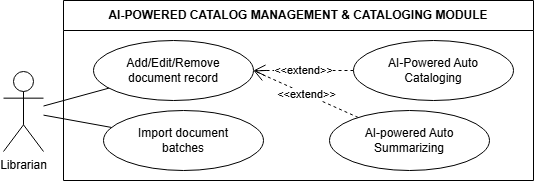
\includegraphics[width=0.8\linewidth]{Images/Quan_ly_danh_muc_bien_muc_AI.png}
    \vspace{10pt}
    \caption{Sơ đồ Use-case Quản lý Danh mục \& Dữ liệu tả AI}
    \label{fig:usecase_catalog}
\end{figure}

\subsubsection{Đặc tả Chi tiết}

% --- UC: ADD / EDIT / DELETE CATALOG RECORD ---
\begin{longtable}{|p{3.5cm}|p{11.5cm}|}
    \hline
    \textbf{Tên Use-case} & \textbf{Thêm / Sửa / Xóa Bản ghi Danh mục} \\
    \hline
    \textbf{Mã Use-case} & UC-CAT-01 \\
    \hline
    \textbf{Tổng quan} & Librarians perform catalog management operations (CRUD), updating metadata or removing lost/damaged copies. \\
    \hline
    \textbf{Tác nhân} & Thủ thư \\
    \hline
    \textbf{Điều kiện tiên quyết} & Librarian is logged into the system. \\
    \hline
    \textbf{Điều kiện kích hoạt} & Librarian navigates to "Catalog Management". \\
    \hline
    \textbf{Luồng sự kiện} & 
    1. System displays list of current catalog items.\newline
    2. Librarian selects action: Add New, Edit, or Delete.\newline
    3. If Delete: Librarian confirms deletion, system checks active loan constraints and executes Soft Delete.\newline
    4. If Add/Edit: System renders item form (Title, Author, ISBN, Category, Copies...).\newline
    \textit{** Extension Points:**}\newline
    - \textbf{[Mở rộng]} Librarian can execute \textit{"Biên mục Tự động qua ISBN"} (UC-CAT-03) to auto-fill form.\newline
    - \textbf{[Mở rộng]} Librarian can execute \textit{"Tóm tắt Tài liệu Tự động"} (UC-CAT-04) if description is missing.\newline
    5. Librarian reviews form fields and clicks "Save".\newline
    6. System validates fields, persists to DB, and displays success alert. \\
    \hline
    \textbf{Điều kiện sau} & Catalog record is updated successfully. \\
    \hline
    \textbf{Ngoại lệ} & 
    Ex1: Required fields missing $\rightarrow$ System highlights missing inputs and requests completion.\newline
    Ex2: Duplicate ISBN code $\rightarrow$ Display "ISBN already exists in catalog". \\
    \hline
    \caption{Đặc tả Use-case: Thêm / Sửa / Xóa Bản ghi Danh mục}
\end{longtable}

\newpage
% --- UC: BATCH CATALOG INGESTION ---
\begin{longtable}{|p{3.5cm}|p{11.5cm}|}
    \hline
    \textbf{Tên Use-case} & \textbf{Nhập Dữ liệu Danh mục Hàng loạt} \\
    \hline
    \textbf{Mã Use-case} & UC-CAT-02 \\
    \hline
    \textbf{Tổng quan} & Allows librarians to import large volumes of catalog records via standard data files (CSV, Excel). \\
    \hline
    \textbf{Tác nhân} & Thủ thư \\
    \hline
    \textbf{Điều kiện tiên quyết} & Librarian is logged into the system. \\
    \hline
    \textbf{Điều kiện kích hoạt} & Librarian clicks "Batch Import" in catalog management. \\
    \hline
    \textbf{Luồng sự kiện} & 
    1. System presents upload interface and sample template file.\newline
    2. Librarian uploads catalog dataset file.\newline
    3. System parses file and displays preview table distinguishing valid vs invalid records.\newline
    4. Librarian confirms import operation.\newline
    5. System writes valid rows to DB and generates execution report (success vs error row counts). \\
    \hline
    \textbf{Điều kiện sau} & Multiple catalog records added to system. \\
    \hline
    \textbf{Ngoại lệ} & 
    Ex1: Unsupported file format $\rightarrow$ System rejects upload: "Unsupported file format".\newline
    Ex2: File contains duplicate ISBNs $\rightarrow$ System skips duplicate lines, logs errors, and imports remaining valid records. \\
    \hline
    \caption{Đặc tả Use-case: Nhập Dữ liệu Danh mục Hàng loạt}
\end{longtable}

% --- UC: AUTOMATED CATALOGING VIA ISBN (AI) ---
\begin{longtable}{|p{3.5cm}|p{11.5cm}|}
    \hline
    \textbf{Tên Use-case} & \textbf{Biên mục Tự động qua ISBN} \\
    \hline
    \textbf{Mã Use-case} & UC-CAT-03 \\
    \hline
    \textbf{Tổng quan} & AI-assisted feature to automatically retrieve and populate book metadata (Title, Author, Publisher, Genre) from external APIs using ISBN lookup. \\
    \hline
    \textbf{Tác nhân} & Thủ thư \\
    \hline
    \textbf{Điều kiện tiên quyết} & Currently executing flow of "Thêm / Sửa / Xóa Bản ghi Danh mục". \\
    \hline
    \textbf{Điều kiện kích hoạt} & Librarian enters ISBN and clicks "Auto-Fetch Metadata". \\
    \hline
    \textbf{Luồng sự kiện} & 
    1. Librarian enters ISBN into corresponding input field.\newline
    2. System dispatches API request to open catalog endpoints (Google Books, Open Library).\newline
    3. System receives JSON response, parsing entity attributes.\newline
    4. System auto-populates form fields with parsed attributes.\newline
    5. Librarian reviews, edits if needed, and proceeds with base cataloging flow. \\
    \hline
    \textbf{Điều kiện sau} & Catalog form is auto-filled, reducing manual entry time for librarians. \\
    \hline
    \textbf{Ngoại lệ} & 
    Ex1: ISBN not found in external databases $\rightarrow$ System alerts "No metadata found, please enter manually".\newline
    Ex2: Third-party API timeout $\rightarrow$ System alerts timeout error and asks librarian to retry. \\
    \hline
    \caption{Đặc tả Use-case: Biên mục Tự động qua ISBN}
\end{longtable}

\newpage
% --- UC: AUTOMATED DOCUMENT SUMMARIZATION (AI) ---
\begin{longtable}{|p{3.5cm}|p{11.5cm}|}
    \hline
    \textbf{Tên Use-case} & \textbf{Tóm tắt Tài liệu Tự động} \\
    \hline
    \textbf{Mã Use-case} & UC-CAT-04 \\
    \hline
    \textbf{Tổng quan} & Uses Large Language Models (LLMs) to automatically generate concise abstract summaries (150-300 words) for catalog items lacking publisher descriptions. \\
    \hline
    \textbf{Tác nhân} & Thủ thư \\
    \hline
    \textbf{Điều kiện tiên quyết} & Executing "Thêm / Sửa / Xóa Bản ghi Danh mục" flow. Title and Author fields populated. \\
    \hline
    \textbf{Điều kiện kích hoạt} & Librarian clicks "Generate AI Summary" in Description field. \\
    \hline
    \textbf{Luồng sự kiện} & 
    1. System collects existing item fields (Title, Author, Category).\newline
    2. System formats prompt payload and sends to AI Engine (e.g., Gemini API).\newline
    3. AI Engine processes payload and returns summary text.\newline
    4. System populates text into Description field, automatically tagging "(AI-generated summary)".\newline
    5. Librarian reviews, edits, or requests regeneration. \\
    \hline
    \textbf{Điều kiện sau} & Item receives concise abstract summary, aiding reader discovery. \\
    \hline
    \textbf{Ngoại lệ} & 
    Ex1: Insufficient metadata input causing inaccurate AI synthesis $\rightarrow$ Generic output returned; librarian discards and clears output. \\
    \hline
    \caption{Đặc tả Use-case: Tóm tắt Tài liệu Tự động}
\end{longtable}

% ======================================================================================
% 4.3 CIRCULATION MANAGEMENT
% ======================================================================================
\subsection{Quản lý Lưu thông Tài liệu}

\subsubsection{Tổng quan}
\begin{figure}[H]
    \centering
    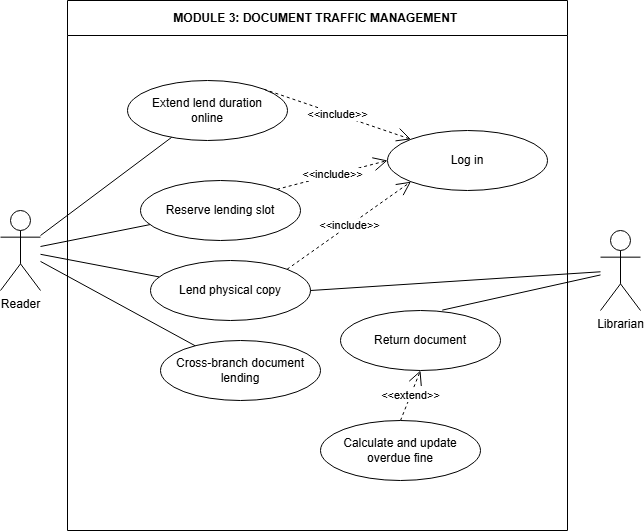
\includegraphics[width=0.8\linewidth]{Images/Quan_ly_luu_thong.png}
    \vspace{10pt}
    \caption{Sơ đồ Use-case Quản lý Lưu thông Tài liệu}
    \label{fig:usecase_circulation}
\end{figure}

\subsubsection{Đặc tả Chi tiết}

% --- UC: BORROW PHYSICAL MATERIAL ---
\begin{longtable}{|p{3.5cm}|p{11.5cm}|}
    \hline
    \textbf{Tên Use-case} & \textbf{Mượn Tài liệu Vật lý} \\
    \hline
    \textbf{Mã Use-case} & UC-CIR-01 \\
    \hline
    \textbf{Tổng quan} & Allows readers to borrow physical materials available at the library counter assisted by a librarian. \\
    \hline
    \textbf{Tác nhân} & Độc giả, Thủ thư \\
    \hline
    \textbf{Điều kiện tiên quyết} & Reader and Librarian possess valid active accounts. Reader has no card suspension or unpaid fines exceeding threshold. \\
    \hline
    \textbf{Điều kiện kích hoạt} & Reader presents items and membership card at circulation desk. \\
    \hline
    \textbf{Luồng sự kiện} & 
    1. \textbf{[Bao gồm]} Librarian logs into circulation module.\newline
    2. Librarian scans Reader membership barcode/ID.\newline
    3. System loads Reader profile, checking borrowing eligibility and fine status.\newline
    4. Librarian scans barcode on each checkout item.\newline
    5. System checks active loan limits against role allowance.\newline
    6. System creates loan record, calculating due dates based on item policy rules.\newline
    7. System updates copy status in inventory to "Checked Out" and decrements available count.\newline
    8. Librarian hands items to Reader; transaction completes. \\
    \hline
    \textbf{Điều kiện sau} & Loan record created in system; transaction logged. \\
    \hline
    \textbf{Ngoại lệ} & 
    Ex1: Reader reached maximum borrowing limit $\rightarrow$ Error alert "Loan limit exceeded"; reader must return existing items first.\newline
    Ex2: Item scanned is on hold for another patron $\rightarrow$ Warning alert; librarian retains item for hold queue. \\
    \hline
    \caption{Đặc tả Use-case: Mượn Tài liệu Vật lý}
\end{longtable}

\newpage
% --- UC: RETURN MATERIAL ---
\begin{longtable}{|p{3.5cm}|p{11.5cm}|}
    \hline
    \textbf{Tên Use-case} & \textbf{Trả Tài liệu} \\
    \hline
    \textbf{Mã Use-case} & UC-CIR-02 \\
    \hline
    \textbf{Tổng quan} & Processes returned physical materials, closes active loan records, and updates copy availability in inventory. \\
    \hline
    \textbf{Tác nhân} & Thủ thư \\
    \hline
    \textbf{Điều kiện tiên quyết} & Items are associated with active open loan records. \\
    \hline
    \textbf{Điều kiện kích hoạt} & Reader returns items at circulation desk. \\
    \hline
    \textbf{Luồng sự kiện} & 
    1. \textbf{[Bao gồm]} Librarian logs into circulation module.\newline
    2. Librarian scans item barcode.\newline
    3. System retrieves associated active loan record.\newline
    4. System compares return date against scheduled due date.\newline
    \textit{** Extension Points:**}\newline
    - \textbf{[Mở rộng]} If return date exceeds due date, system triggers "Tính và Thu Phạt Quá hạn" (UC-CIR-03).\newline
    5. Updates loan status to "Completed".\newline
    6. System verifies hold queue status for returned item:\newline
    - If hold exists: Set status to "Awaiting Pickup" and send notification to next patron.\newline
    - If no hold: Set status to "Available" and increment copy inventory count. \\
    \hline
    \textbf{Điều kiện sau} & Loan record closed. Item marked available for next transaction. \\
    \hline
    \textbf{Ngoại lệ} & 
    Ex1: Barcode damaged/unreadable $\rightarrow$ Librarian performs manual lookup by title and borrower ID. \\
    \hline
    \caption{Đặc tả Use-case: Trả Tài liệu}
\end{longtable}

% --- UC: CALCULATE OVERDUE FINES ---
\begin{longtable}{|p{3.5cm}|p{11.5cm}|}
    \hline
    \textbf{Tên Use-case} & \textbf{Tính và Thu Phạt Quá hạn} \\
    \hline
    \textbf{Mã Use-case} & UC-CIR-03 \\
    \hline
    \textbf{Tổng quan} & Automatically computes fine amounts when items are returned past due dates. \\
    \hline
    \textbf{Tác nhân} & Thủ thư \\
    \hline
    \textbf{Điều kiện tiên quyết} & Triggered from "Trả Tài liệu" when system detects overdue return. \\
    \hline
    \textbf{Điều kiện kích hoạt} & Return Date > Due Date in loan record. \\
    \hline
    \textbf{Luồng sự kiện} & 
    1. System computes overdue days: (Actual Return Date - Due Date).\newline
    2. Fetches daily fine rate applicable to material type (configured by Admin).\newline
    3. Calculates total fine amount (Overdue Days $\times$ Daily Rate).\newline
    4. Displays fine calculation on librarian view.\newline
    5. Librarian notifies reader. If reader pays immediately, receipt is generated; otherwise fine is posted to reader ledger. \\
    \hline
    \textbf{Điều kiện sau} & Fine record updated on reader profile or marked as paid. \\
    \hline
    \textbf{Ngoại lệ} & 
    Ex1: Official holidays fall within overdue range $\rightarrow$ System automatically excludes official library holidays from overdue day count. \\
    \hline
    \caption{Đặc tả Use-case: Tính và Thu Phạt Quá hạn}
\end{longtable}

\newpage
% --- UC: ONLINE LOAN RENEWAL ---
\begin{longtable}{|p{3.5cm}|p{11.5cm}|}
    \hline
    \textbf{Tên Use-case} & \textbf{Gia hạn Mượn Trực tuyến} \\
    \hline
    \textbf{Mã Use-case} & UC-CIR-04 \\
    \hline
    \textbf{Tổng quan} & Allows readers to extend loan periods online without physically visiting the library. \\
    \hline
    \textbf{Tác nhân} & Độc giả \\
    \hline
    \textbf{Điều kiện tiên quyết} & Item is not overdue and renewal limit has not been reached. \\
    \hline
    \textbf{Điều kiện kích hoạt} & Reader clicks "Renew" in active loans dashboard. \\
    \hline
    \textbf{Luồng sự kiện} & 
    1. \textbf{[Bao gồm]} Reader logs into system portal.\newline
    2. System verifies renewal eligibility:\newline
    - Has maximum renewal limit been reached for item?\newline
    - Does an active hold request exist from another user?\newline
    3. If eligible, system extends due date by configured extension period.\newline
    4. System updates loan record and increments renewal counter.\newline
    5. Displays "Renewal Successful" along with new due date. \\
    \hline
    \textbf{Điều kiện sau} & Item due date is extended. \\
    \hline
    \textbf{Ngoại lệ} & 
    Ex1: Item has active hold request $\rightarrow$ System rejects renewal: "Item requested by another user, please return on time". \\
    \hline
    \caption{Đặc tả Use-case: Gia hạn Mượn Trực tuyến}
\end{longtable}

% --- UC: PLACE ITEM HOLD ---
\begin{longtable}{|p{3.5cm}|p{11.5cm}|}
    \hline
    \textbf{Tên Use-case} & \textbf{Đặt Giữ chỗ Tài liệu} \\
    \hline
    \textbf{Mã Use-case} & UC-CIR-05 \\
    \hline
    \textbf{Tổng quan} & Enables readers to join a reservation queue for items currently out of stock. \\
    \hline
    \textbf{Tác nhân} & Độc giả \\
    \hline
    \textbf{Điều kiện tiên quyết} & Target item status is "All Copies Checked Out". \\
    \hline
    \textbf{Điều kiện kích hoạt} & Reader clicks "Place Hold" on item detail view. \\
    \hline
    \textbf{Luồng sự kiện} & 
    1. \textbf{[Bao gồm]} Reader logs into system portal.\newline
    2. System verifies Reader does not currently hold an active loan for same title.\newline
    3. System appends Reader ID to item reservation queue.\newline
    4. Interface displays "Hold Placed Successfully" showing queue position.\newline
    5. Upon item return, system holds copy and alerts queue position \#1 patron. \\
    \hline
    \textbf{Điều kiện sau} & Reservation saved; renewal blocked for current borrower. \\
    \hline
    \textbf{Ngoại lệ} & 
    Ex1: Reader has unpaid fines or card suspension $\rightarrow$ System rejects hold request. \\
    \hline
    \caption{Đặc tả Use-case: Place Item Hold}
\end{longtable}

\newpage
% --- UC: INTER-BRANCH LOAN REQUEST ---
\begin{longtable}{|p{3.5cm}|p{11.5cm}|}
    \hline
    \textbf{Tên Use-case} & \textbf{Yêu cầu Mượn Liên Chi nhánh} \\
    \hline
    \textbf{Mã Use-case} & UC-CIR-06 \\
    \hline
    \textbf{Tổng quan} & Allows readers to request item transfers from another branch library to their local campus library for pickup. \\
    \hline
    \textbf{Tác nhân} & Độc giả \\
    \hline
    \textbf{Điều kiện tiên quyết} & Multi-branch network enabled. Item unavailable locally but available at another branch. \\
    \hline
    \textbf{Điều kiện kích hoạt} & Reader clicks "Request Inter-Branch Transfer" on book detail page. \\
    \hline
    \textbf{Luồng sự kiện} & 
    1. \textbf{[Bao gồm]} Reader logs into system portal.\newline
    2. System prompts Reader to select preferred pickup branch.\newline
    3. Reader confirms request.\newline
    4. System creates inter-branch transfer ticket sent to holding branch.\newline
    5. Holding librarian packages item; status changes to "In Transit".\newline
    6. Upon arrival at destination branch, automated notification alerts Reader for pickup. \\
    \hline
    \textbf{Điều kiện sau} & Physical transfer logged and inventory updated across branches. \\
    \hline
    \textbf{Ngoại lệ} & 
    Ex1: Last available copy borrowed before request processing $\rightarrow$ Cancel request and suggest standard hold queue. \\
    \hline
    \caption{Đặc tả Use-case: Yêu cầu Mượn Liên Chi nhánh}
\end{longtable}

% ======================================================================================
% 4.4 RESOURCE ACCESS AND EXPLOITATION
% ======================================================================================
\subsection{Truy cập và Khai thác Tài nguyên}

\subsubsection{Tổng quan}
\begin{figure}[H]
    \centering
    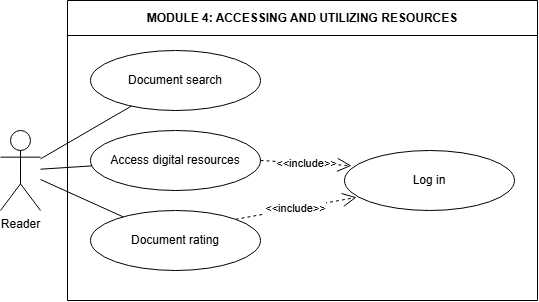
\includegraphics[width=0.8\linewidth]{Images/Truy_cap_khai_thac_tai_nguyen.png}
    \vspace{10pt}
    \caption{Sơ đồ Use-case Truy cập \& Khai thác Tài nguyên}
    \label{fig:usecase_exploration}
\end{figure}

\subsubsection{Đặc tả Chi tiết}

% --- UC: DOCUMENT SEARCH ---
\begin{longtable}{|p{3.5cm}|p{11.5cm}|}
    \hline
    \textbf{Tên Use-case} & \textbf{Tìm kiếm Danh mục Tài liệu} \\
    \hline
    \textbf{Mã Use-case} & UC-EXP-01 \\
    \hline
    \textbf{Tổng quan} & Allows readers to search library catalog records via keywords (Title, Author, Genre, ISBN). \\
    \hline
    \textbf{Tác nhân} & Độc giả (Bao gồm cả khách chưa xác thực) \\
    \hline
    \textbf{Điều kiện tiên quyết} & System online with active DB connection. \\
    \hline
    \textbf{Điều kiện kích hoạt} & Reader inputs query string and submits search. \\
    \hline
    \textbf{Luồng sự kiện} & 
    1. Reader selects search filter scope (All, Title, Author...) and enters query.\newline
    2. System queries catalog database indexes.\newline
    3. System returns paginated match results.\newline
    4. Renders item cards (Cover image, Title, Author, Year, Availability Status).\newline
    5. Reader clicks item card to open detail view. \\
    \hline
    \textbf{Điều kiện sau} & System state remains unchanged. \\
    \hline
    \textbf{Ngoại lệ} & 
    Ex1: No items match query $\rightarrow$ Display "No results found" with spelling/keyword suggestions. \\
    \hline
    \caption{Đặc tả Use-case: Tìm kiếm Danh mục Tài liệu}
\end{longtable}

% \newpage
% % --- UC: ACCESS DIGITAL RESOURCES (chưa triển khai) ---
% \begin{longtable}{|p{3.5cm}|p{11.5cm}|}
%     \hline
%     \textbf{Tên Use-case} & \textbf{Access Digital Resources} \\\
%     \hline
%     \textbf{Mã Use-case} & UC-EXP-02 \\\
%     \hline
%     \textbf{Tổng quan} & Enables readers to stream/read digital materials (E-books, PDFs) online. \\\
%     \hline
%     \textbf{Tác nhân} & Độc giả \\\
%     \hline
%     \textbf{Điều kiện tiên quyết} & Item possesses digital file format. \\\
%     \hline
%     \textbf{Điều kiện kích hoạt} & Reader clicks ``Read Online'' on item page. \\\
%     \hline
%     \textbf{Luồng sự kiện} &
%     1. \textbf{[Bao gồm]} System checks authentication, prompting login if needed.\newline
%     2. System verifies Reader digital access privileges.\newline
%     3. System checks concurrent license access limits (e.g., max 5 concurrent readers).\newline
%     4. If approved, opens embedded web PDF/ePUB viewer.\newline
%     5. Logs digital reading session. \\\
%     \hline
%     \textbf{Điều kiện sau} & Digital reading session established. \\\
%     \hline
%     \textbf{Ngoại lệ} &
%     Ex1: Concurrent user limit reached $\rightarrow$ Display ``All digital licenses currently in use. Please try again later''. \\\
%     \hline
%     \caption{Đặc tả Use-case: Access Digital Resources (not implemented)}
% \end{longtable}

% --- UC: RATE AND REVIEW MATERIALS ---
\begin{longtable}{|p{3.5cm}|p{11.5cm}|}
    \hline
    \textbf{Tên Use-case} & \textbf{Đánh giá và Nhận xét Tài liệu} \\
    \hline
    \textbf{Mã Use-case} & UC-EXP-03 \\
    \hline
    \textbf{Tổng quan} & Allows readers to leave 1-5 star ratings and written reviews for items they have read. \\
    \hline
    \textbf{Tác nhân} & Độc giả \\
    \hline
    \textbf{Điều kiện tiên quyết} & Reader has borrowed the physical item (preventing spam). \\
    \hline
    \textbf{Điều kiện kích hoạt} & Reader clicks "Write a Review" on book page. \\
    \hline
    \textbf{Luồng sự kiện} & 
    1. \textbf{[Bao gồm]} System verifies login status.\newline
    2. System verifies loan history against target item.\newline
    3. Renders rating selector (1-5 stars) and review text area.\newline
    4. Reader submits rating and optional review.\newline
    5. System checks content moderation filters.\newline
    6. Saves rating, updates item average rating score.\newline
    7. Displays success alert and refreshes view. \\
    \hline
    \textbf{Điều kiện sau} & Review saved; average item score updated. \\
    \hline
    \textbf{Ngoại lệ} & 
    Ex1: Reader has not borrowed item $\rightarrow$ Hide review button or display "You must borrow this item before submitting a review".\newline
    Ex2: Review contains profanity $\rightarrow$ Block submission with moderation warning. \\
    \hline
    \caption{Đặc tả Use-case: Đánh giá và Nhận xét Tài liệu}
\end{longtable}

% ======================================================================================
% 4.5 INTELLIGENT INTERACTION AND AI
% ======================================================================================
\subsection{Tương tác Thông minh}

\subsubsection{Tổng quan}
\begin{figure}[H]
    \centering
    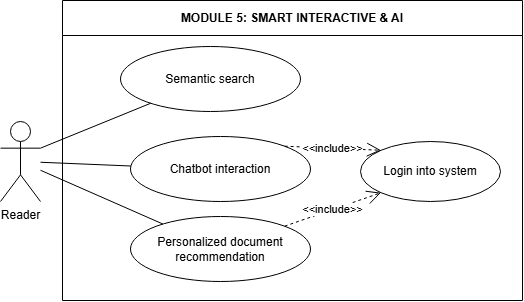
\includegraphics[width=0.8\linewidth]{Images/Tuong_tac_thong_minh_AI.png}
    \vspace{10pt}
    \caption{Sơ đồ Use-case Tương tác Thông minh \& AI}
    \label{fig:usecase_smart_ai}
\end{figure}

\subsubsection{Đặc tả Chi tiết}

% --- UC: NATURAL LANGUAGE SEARCH ---
\begin{longtable}{|p{3.5cm}|p{11.5cm}|}
    \hline
    \textbf{Tên Use-case} & \textbf{Tìm kiếm Ngôn ngữ Tự nhiên} \\
    \hline
    \textbf{Mã Use-case} & UC-AI-01 \\
    \hline
    \textbf{Tổng quan} & Allows readers to search catalog items using conversational phrases (e.g., "introductory artificial intelligence textbooks") rather than exact keywords. \\
    \hline
    \textbf{Tác nhân} & Độc giả \\
    \hline
    \textbf{Điều kiện tiên quyết} & System AI NLP module operational. \\
    \hline
    \textbf{Điều kiện kích hoạt} & Reader inputs phrase into Smart Search bar and submits. \\
    \hline
    \textbf{Luồng sự kiện} & 
    1. Reader enters natural language query.\newline
    2. NLP module processes query via Intent Analysis \& Entity Extraction (genre, topic, target level).\newline
    3. System converts entities into vector embeddings or metadata filter trees.\newline
    4. Executes vector similarity search (pgvector) and semantic ranking.\newline
    5. Renders ranked search results sorted by semantic relevance scores. \\
    \hline
    \textbf{Điều kiện sau} & Semantic search results rendered with related topic tags. \\
    \hline
    \textbf{Ngoại lệ} & 
    Ex1: Irrelevant or meaningless phrase $\rightarrow$ AI assistant prompts "No matching documents found. Try phrases like...".\newline
    Ex2: AI service offline $\rightarrow$ System falls back to full-text keyword search and alerts "Smart search temporarily under maintenance". \\
    \hline
    \caption{Đặc tả Use-case: Tìm kiếm Ngôn ngữ Tự nhiên}
\end{longtable}

\newpage
% --- UC: CHATBOT VIRTUAL ASSISTANT ---
\begin{longtable}{|p{3.5cm}|p{11.5cm}|}
    \hline
    \textbf{Tên Use-case} & \textbf{Tương tác với Chatbot Trợ lý ảo} \\
    \hline
    \textbf{Mã Use-case} & UC-AI-02 \\
    \hline
    \textbf{Tổng quan} & Readers interact with an AI Chatbot for policy inquiries, opening hours, or checking personal account loan status. \\
    \hline
    \textbf{Tác nhân} & Độc giả \\
    \hline
    \textbf{Điều kiện tiên quyết} & AI Chatbot service online. \\
    \hline
    \textbf{Điều kiện kích hoạt} & Reader opens Chatbot widget window. \\
    \hline
    \textbf{Luồng sự kiện} & 
    1. \textbf{[Bao gồm]} System prompts login if unauthenticated for personalized responses.\newline
    2. Chatbot interface displays welcome message and quick action buttons (FAQ, My Loans, Book Suggestions).\newline
    3. Reader types message or selects quick prompt.\newline
    4. Chatbot (LLM) analyzes context:\newline
    - General FAQ: Retrieves answer from RAG knowledge base.\newline
    - Account query (e.g., "What books do I owe?"): Chatbot queries backend API using Reader ID and synthesizes response.\newline
    5. Renders conversational response in chat widget. \\
    \hline
    \textbf{Điều kiện sau} & Chat transcript saved for audit logging and AI refinement. \\
    \hline
    \textbf{Ngoại lệ} & 
    Ex1: Query out of scope $\rightarrow$ Response: "I am a library assistant. Please contact staff at hotline for special inquiries." \\
    \hline
    \caption{Đặc tả Use-case: Tương tác với Chatbot Trợ lý ảo}
\end{longtable}

\newpage
% --- UC: PERSONALIZED RECOMMENDATIONS ---
% \begin{longtable}{|p{3.5cm}|p{11.5cm}|}
%     \hline
%     \textbf{Tên Use-case} & \textbf{Xem Gợi ý Cá nhân hóa} \\
%     \hline
%     \textbf{Mã Use-case} & UC-AI-03 \\
%     \hline
%     \textbf{Tổng quan} & Provides readers with tailored book recommendations generated from loan history, search logs, and collaborative user behavior. \\
%     \hline
%     \textbf{Tác nhân} & Độc giả \\
%     \hline
%     \textbf{Điều kiện tiên quyết} & AI Recommendation engine online. \\
%     \hline
%     \textbf{Điều kiện kích hoạt} & Reader opens homepage dashboard or "Recommended For You" view. \\
%     \hline
%     \textbf{Luồng sự kiện} & 
%     1. \textbf{[Bao gồm]} Reader logs into system.\newline
%     2. System aggregates user signals: loan history, recent searches, ratings.\newline
%     3. System sends telemetry to Recommendation Engine.\newline
%     4. Engine executes Collaborative Filtering and Content-Based Filtering models.\newline
%     5. Filters out items currently checked out or held by user.\newline
%     6. Displays "Recommended For You" grid with brief rationale tags (e.g., "Because you read Title X..."). \\
%     \hline
%     \textbf{Điều kiện sau} & Interface presents personalized recommendations. \\
%     \hline
%     \textbf{Ngoại lệ} & 
%     Ex1: New account with no history (Cold Start) $\rightarrow$ Display "Trending Titles" or "New Arrivals" fallback. \\
%     \hline
%     \caption{Đặc tả Use-case: Xem Gợi ý Cá nhân hóa}
% \end{longtable}

% ======================================================================================
% 4.6 NOTIFICATIONS AND COMMUNICATION
% ======================================================================================
\subsection{Thông báo và Tương tác}

\subsubsection{Tổng quan}
\begin{figure}[H]
    \centering
    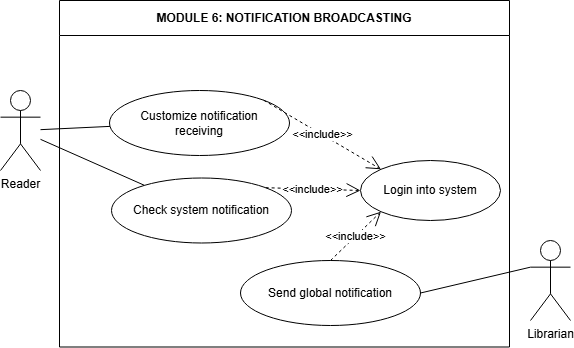
\includegraphics[width=0.8\linewidth]{Images/Thong_bao_truyen_thong.png}
    \vspace{10pt}
    \caption{Sơ đồ Use-case Thông báo \& Tương tác}
    \label{fig:usecase_notifications}
\end{figure}

\subsubsection{Đặc tả Chi tiết}

% --- UC: NOTIFICATION PREFERENCES ---
\begin{longtable}{|p{3.5cm}|p{11.5cm}|}
    \hline
    \textbf{Tên Use-case} & \textbf{Cấu hình Tùy chọn Thông báo} \\
    \hline
    \textbf{Mã Use-case} & UC-NOT-01 \\
    \hline
    \textbf{Tổng quan} & Allows readers to customize delivery channels (Email, SMS, In-app) and event alerts (Due Reminders, Hold Pickups, System News). \\
    \hline
    \textbf{Tác nhân} & Độc giả \\
    \hline
    \textbf{Điều kiện tiên quyết} & Reader possesses valid account. \\
    \hline
    \textbf{Điều kiện kích hoạt} & Reader opens "Notification Settings" in profile view. \\
    \hline
    \textbf{Luồng sự kiện} & 
    1. \textbf{[Bao gồm]} System prompts login verification.\newline
    2. System loads and renders current notification configuration toggles.\newline
    3. Reader toggles preferences for channels and event categories.\newline
    4. Reader clicks "Save Settings".\newline
    5. System validates and persists configuration to DB.\newline
    6. Displays "Notification preferences saved successfully". \\
    \hline
    \textbf{Điều kiện sau} & System dispatches notifications strictly per user preferences. \\
    \hline
    \textbf{Ngoại lệ} & 
    Ex1: SMS toggled on without phone number in profile $\rightarrow$ Warning alert requesting phone number update first. \\
    \hline
    \caption{Đặc tả Use-case: Cấu hình Tùy chọn Thông báo}
\end{longtable}

\newpage
% --- UC: VIEW SYSTEM NOTIFICATIONS ---
\begin{longtable}{|p{3.5cm}|p{11.5cm}|}
    \hline
    \textbf{Tên Use-case} & \textbf{Xem Thông báo Hệ thống} \\
    \hline
    \textbf{Mã Use-case} & UC-NOT-02 \\
    \hline
    \textbf{Tổng quan} & Enables users to review alerts and reminders directly within the web app interface. \\
    \hline
    \textbf{Tác nhân} & Độc giả \\
    \hline
    \textbf{Điều kiện tiên quyết} & User has incoming notification records. \\
    \hline
    \textbf{Điều kiện kích hoạt} & User clicks "Bell" icon (Notification Center) on top navbar. \\
    \hline
    \textbf{Luồng sự kiện} & 
    1. \textbf{[Bao gồm]} System verifies user login.\newline
    2. Queries notification table by User ID sorted by timestamp desc.\newline
    3. Renders notification panel distinguishing read vs unread items.\newline
    4. User clicks notification item to view details.\newline
    5. System marks notification as "Read" and decrements unread badge count. \\
    \hline
    \textbf{Điều kiện sau} & Notification status updated to "Read". \\
    \hline
    \textbf{Ngoại lệ} & 
    Ex1: Notification panel empty $\rightarrow$ Display "You have no new notifications". \\
    \hline
    \caption{Đặc tả Use-case: Xem Thông báo Hệ thống}
\end{longtable}

% --- UC: BROADCAST MASS NOTIFICATIONS ---
\begin{longtable}{|p{3.5cm}|p{11.5cm}|}
    \hline
    \textbf{Tên Use-case} & \textbf{Phát Thông báo Đại chúng} \\
    \hline
    \textbf{Mã Use-case} & UC-NOT-03 \\
    \hline
    \textbf{Tổng quan} & Allows Librarians to create and send general announcements (holiday closures, maintenance, policy updates) to all or targeted reader groups. \\
    \hline
    \textbf{Tác nhân} & Thủ thư \\
    \hline
    \textbf{Điều kiện tiên quyết} & Librarian active with broadcast privileges. \\
    \hline
    \textbf{Điều kiện kích hoạt} & Librarian accesses "Communication Management" tool in admin portal. \\
    \hline
    \textbf{Luồng sự kiện} & 
    1. \textbf{[Bao gồm]} System verifies Librarian session and privileges.\newline
    2. Renders broadcast creation form.\newline
    3. Librarian inputs: Title, Content, Channel (In-app, Email), Target Group (All, Students, Faculty).\newline
    4. Librarian clicks "Send Broadcast".\newline
    5. System prompts confirmation dialog.\newline
    6. System enqueues notification payload in Message Queue for dispatch.\newline
    7. Displays success confirmation and logs administrative action. \\
    \hline
    \textbf{Điều kiện sau} & Broadcast logged and dispatched to target users. \\
    \hline
    \textbf{Ngoại lệ} & 
    Ex1: Empty title or body $\rightarrow$ Disable send button and alert "Please enter complete broadcast content". \\
    \hline
    \caption{Đặc tả Use-case: Phát Thông báo Đại chúng}
\end{longtable}

% ======================================================================================
% 4.7 REPORTING AND SYSTEM ADMINISTRATION
% ======================================================================================
\subsection{Báo cáo và Quản trị Hệ thống}

\subsubsection{Tổng quan}
\begin{figure}[H]
    \centering
    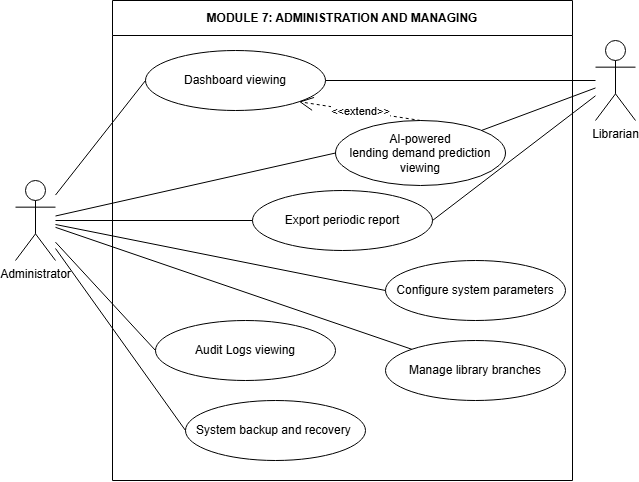
\includegraphics[width=0.8\linewidth]{Images/Bao_cao_quan_tri.png}
    \vspace{10pt}
    \caption{Sơ đồ Use-case Báo cáo \& Quản trị Hệ thống}
    \label{fig:usecase_admin}
\end{figure}

\subsubsection{Đặc tả Chi tiết}

% --- UC: VIEW DASHBOARD ---
\begin{longtable}{|p{3.5cm}|p{11.5cm}|}
    \hline
    \textbf{Tên Use-case} & \textbf{Xem Bảng điều khiển Vận hành} \\
    \hline
    \textbf{Mã Use-case} & UC-ADM-01 \\
    \hline
    \textbf{Tổng quan} & Provides real-time dashboard visualization of key operational metrics (active loans, overdue items, traffic). \\
    \hline
    \textbf{Tác nhân} & Quản trị viên (Admin), Thủ thư \\
    \hline
    \textbf{Điều kiện tiên quyết} & User logged in as Admin or Librarian. \\
    \hline
    \textbf{Điều kiện kích hoạt} & User opens administrative homepage. \\
    \hline
    \textbf{Luồng sự kiện} & 
    1. System receives request.\newline
    2. Queries DB aggregating real-time daily/weekly metrics.\newline
    3. Renders charts and metric summary cards. \\
    \hline
    \textbf{Điều kiện sau} & System data state remains unchanged. \\
    \hline
    \textbf{Ngoại lệ} & 
    Ex1: DB load high $\rightarrow$ Display cached dashboard data with refresh timestamp notice. \\
    \hline
    \caption{Đặc tả Use-case: Xem Bảng điều khiển Vận hành}
\end{longtable}

\newpage
% --- UC: EXPORT PERIODIC REPORTS ---
\begin{longtable}{|p{3.5cm}|p{11.5cm}|}
    \hline
    \textbf{Tên Use-case} & \textbf{Xuất Báo cáo Thống kê Định kỳ} \\
    \hline
    \textbf{Mã Use-case} & UC-ADM-02 \\
    \hline
    \textbf{Tổng quan} & Supports exporting library metrics and audit data to standard formats (PDF, CSV, Excel) for archiving and reporting. \\
    \hline
    \textbf{Tác nhân} & Quản trị viên (Admin), Thủ thư \\
    \hline
    \textbf{Điều kiện tiên quyết} & User logged in with report export privileges. \\
    \hline
    \textbf{Điều kiện kích hoạt} & User opens "Statistical Reports" and selects "Export Data". \\
    \hline
    \textbf{Luồng sự kiện} & 
    1. System renders export configuration modal.\newline
    2. User selects report type (Top Borrowed, Fine Income, Overdues), date range, and export format.\newline
    3. User clicks "Export".\newline
    4. System compiles dataset and generates file artifact.\newline
    5. File download triggers automatically on client browser. \\
    \hline
    \textbf{Điều kiện sau} & Report artifact generated and downloaded. \\
    \hline
    \textbf{Ngoại lệ} & 
    Ex1: No records match date range $\rightarrow$ Warning alert "No data available for selected period". \\
    \hline
    \caption{Đặc tả Use-case: Xuất Báo cáo Thống kê Định kỳ}
\end{longtable}

% --- UC: CONFIGURE SYSTEM PARAMETERS ---
\begin{longtable}{|p{3.5cm}|p{11.5cm}|}
    \hline
    \textbf{Tên Use-case} & \textbf{Cấu hình Tham số Hệ thống} \\
    \hline
    \textbf{Mã Use-case} & UC-ADM-04 \\
    \hline
    \textbf{Tổng quan} & Configures core operational library rules: loan limits, loan durations, and daily overdue fine rates per item type. \\
    \hline
    \textbf{Tác nhân} & Quản trị viên (Admin) \\
    \hline
    \textbf{Điều kiện tiên quyết} & Admin logged into system. \\
    \hline
    \textbf{Điều kiện kích hoạt} & Admin opens "System Settings". \\
    \hline
    \textbf{Luồng sự kiện} & 
    1. System displays current global system settings.\newline
    2. Admin modifies values (e.g., fine rate adjustment).\newline
    3. Admin clicks "Save Configuration".\newline
    4. System validates parameters.\newline
    5. Updates DB and records entry in Audit Log. \\
    \hline
    \textbf{Điều kiện sau} & System calculations immediately apply updated configuration settings. \\
    \hline
    \textbf{Ngoại lệ} & 
    Ex1: Invalid parameter input (negative values) $\rightarrow$ Reject save and display validation error. \\
    \hline
    \caption{Đặc tả Use-case: Cấu hình Tham số Hệ thống}
\end{longtable}

% --- UC: MANAGE BRANCHES ---
\begin{longtable}{|p{3.5cm}|p{11.5cm}|}
    \hline
    \textbf{Tên Use-case} & \textbf{Quản lý Chi nhánh Thư viện} \\
    \hline
    \textbf{Mã Use-case} & UC-ADM-05 \\
    \hline
    \textbf{Tổng quan} & Adds, edits, or deactivates affiliated branch libraries, managing physical network topology. \\
    \hline
    \textbf{Tác nhân} & Quản trị viên (Admin) \\
    \hline
    \textbf{Điều kiện tiên quyết} & Admin logged into system. \\
    \hline
    \textbf{Điều kiện kích hoạt} & Admin selects "Branch Management". \\
    \hline
    \textbf{Luồng sự kiện} & 
    1. System renders active branch list.\newline
    2. Admin selects Add New, Edit, or Remove.\newline
    3. Admin enters branch attributes (Name, Address, Contact, Manager).\newline
    4. Admin clicks "Save".\newline
    5. System updates records and displays success alert. \\
    \hline
    \textbf{Điều kiện sau} & Branch directory updated. \\
    \hline
    \textbf{Ngoại lệ} & 
    Ex1: Attempting to delete branch with active inventory or staff $\rightarrow$ System prevents deletion to maintain referential integrity. \\
    \hline
    \caption{Đặc tả Use-case: Quản lý Chi nhánh Thư viện}
\end{longtable}

\newpage
% --- UC: VIEW AUDIT LOGS ---
\begin{longtable}{|p{3.5cm}|p{11.5cm}|}
    \hline
    \textbf{Tên Use-case} & \textbf{Xem Nhật ký Kiểm toán} \\
    \hline
    \textbf{Mã Use-case} & UC-ADM-06 \\
    \hline
    \textbf{Tổng quan} & Inspects historical logs of critical administrative actions (who did what, when) for security auditing. \\
    \hline
    \textbf{Tác nhân} & Quản trị viên (Admin) \\
    \hline
    \textbf{Điều kiện tiên quyết} & Admin logged into system. \\
    \hline
    \textbf{Điều kiện kích hoạt} & Admin accesses "Audit Logs" menu. \\
    \hline
    \textbf{Luồng sự kiện} & 
    1. System retrieves records from Audit Log table.\newline
    2. Renders event stream sorted by timestamp desc.\newline
    3. Admin filters log stream by actor, date range, or risk severity (Info, Warning, Critical).\newline
    4. Admin views detailed payload diffs (Old Data vs New Data). \\
    \hline
    \textbf{Điều kiện sau} & Read-only view; system state remains unchanged. \\
    \hline
    \textbf{Ngoại lệ} & No major exceptions. \\
    \hline
    \caption{Đặc tả Use-case: Xem Nhật ký Kiểm toán}
\end{longtable}

% --- UC: SAO LƯU VÀ PHỤC HỒI DỮ LIỆU ---
% \begin{longtable}{|p{3.5cm}|p{11.5cm}|}
%     \hline
%     \textbf{Tên Use-case} & \textbf{Sao lưu và phục hồi dữ liệu} \\
%     \hline
%     \textbf{Mã Use-case} & UC-ADM-07 \\
%     \hline
%     \textbf{Tổng quan} & Đảm bảo an toàn dữ liệu hệ thống bằng cách sao lưu thủ công/tự động và khôi phục lại khi có sự cố. \\
%     \hline
%     \textbf{Tác nhân} & Quản trị viên (Admin) \\
%     \hline
%     \textbf{Tiền điều kiện} & Admin đã đăng nhập với quyền hạn cao nhất. \\
%     \hline
%     \textbf{Điều kiện kích hoạt} & Admin truy cập mục "Quản trị dữ liệu". \\
%     \hline
%     \textbf{Các bước} & 
%     1. Màn hình hiển thị danh sách các bản sao lưu đã có và nút chức năng.\newline
%     2. Nếu chọn Sao lưu (Backup): Admin nhấn nút, hệ thống nén dữ liệu hiện tại và lưu trữ lên Server/Cloud.\newline
%     3. Nếu chọn Phục hồi (Restore): Admin chọn một bản sao lưu cũ, nhập mật khẩu cấp cao để xác nhận.\newline
%     4. Hệ thống tiến hành ghi đè dữ liệu hiện tại bằng dữ liệu từ bản sao lưu.\newline
%     5. Hệ thống khởi động lại dịch vụ và thông báo quá trình hoàn tất. \\
%     \hline
%     \textbf{Hậu điều kiện} & Dữ liệu được lưu trữ an toàn hoặc hệ thống được hoàn nguyên về trạng thái cũ. \\
%     \hline
%     \textbf{Xử lý ngoại lệ} & 
%     Ex1: Bản sao lưu bị hỏng (Corrupted) $\rightarrow$ Hệ thống cảnh báo lỗi khi cố gắng Restore và hủy bỏ tiến trình để bảo vệ dữ liệu hiện tại. \\
%     \hline
%     \caption{Đặc tả Use-case Sao lưu và phục hồi dữ liệu}
% \end{longtable}
\newpage
\section{Phân tích và Thiết kế Hệ thống}
\subsection{Kiến trúc Hệ thống}

Để trực quan hóa các luồng dữ liệu và sự phân tách vai trò giữa các thành phần công nghệ trong Hệ thống Quản lý Thư viện Trực tuyến, cấu trúc tổng thể được mô hình hóa qua sơ đồ kiến trúc dưới đây:

\begin{figure}[H]
	\centering
	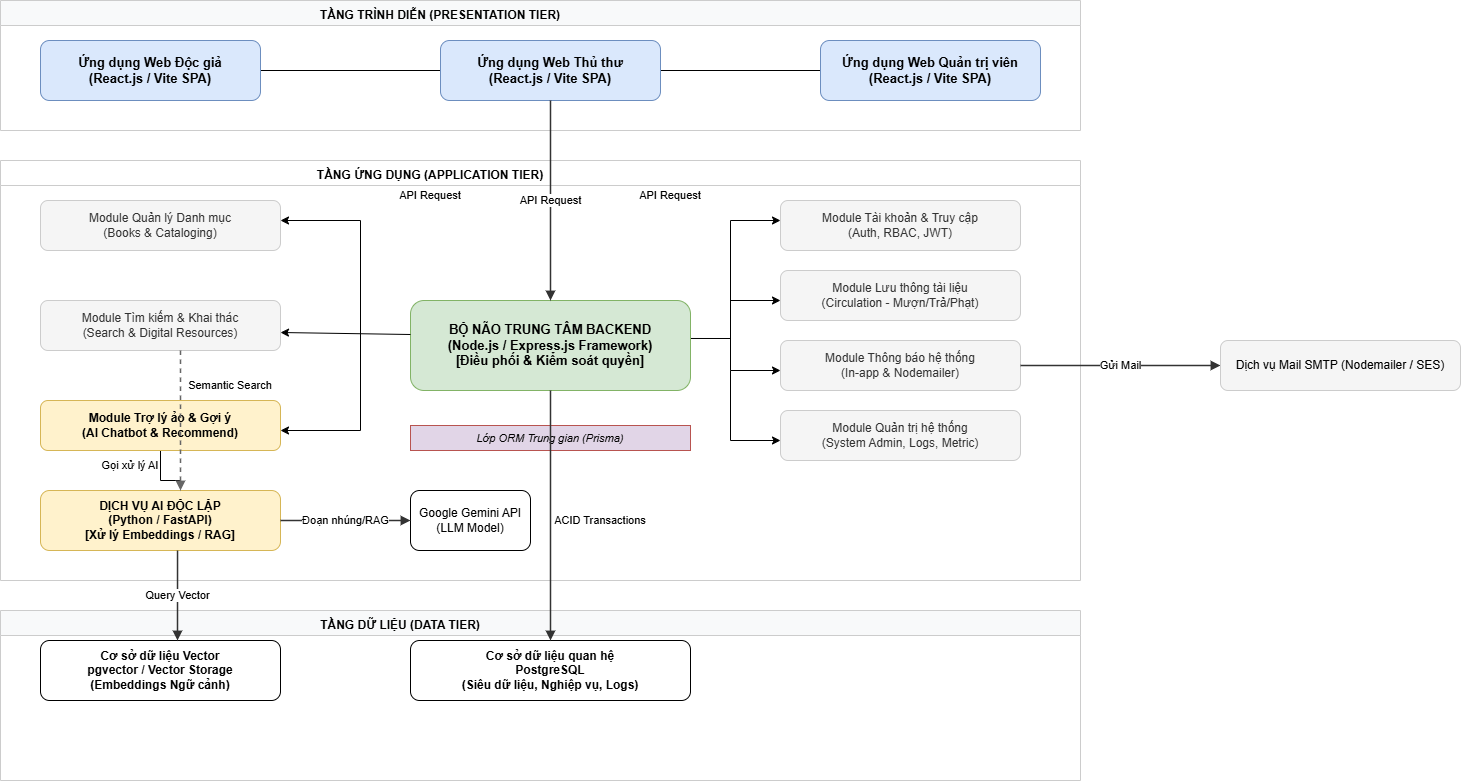
\includegraphics[width=0.6\linewidth]{Images/kientruchethong.png}
	\vspace{10pt}
	\caption{Sơ đồ Kiến trúc Tổng thể của Hệ thống Quản lý Thư viện Trực tuyến}
	\label{fig:system_architecture}
\end{figure}

Tổng thể, kiến trúc của Hệ thống Quản lý Thư viện Trực tuyến được xây dựng dựa trên Mô hình 3 Tầng tiêu chuẩn (Three-Tier Architecture), kết hợp linh hoạt với mô hình Kiến trúc Hướng Dịch vụ (SOA) để tối ưu hóa các tác vụ Trí tuệ Nhân tạo độc lập. Ba tầng nền tảng của dự án bao gồm: Tầng Giao diện (Presentation Tier), Tầng Ứng dụng (Application Tier) và Tầng Dữ liệu (Data Tier).

Việc áp dụng mô hình này đảm bảo sự phân tách rõ ràng trách nhiệm giữa tương tác giao diện người dùng, logic nghiệp vụ thư viện và các hệ quản trị cơ sở dữ liệu. Nhờ tính độc lập cao giữa các tầng, nhóm phát triển có thể dễ dàng bảo trì hoặc nâng cấp độc lập từng thành phần (như tối ưu hóa thuật toán AI hoặc cập nhật giao diện web) mà không làm gián đoạn các quy trình vận hành cốt lõi bên dưới.

\subsubsection{Tầng Giao diện (Presentation Tier)}
Đóng vai trò là điểm tiếp xúc trực tiếp cho người dùng cuối, tầng này được triển khai dưới dạng một Ứng dụng Trang Đơn (SPA) mạnh mẽ sử dụng thư viện React.js và công cụ đóng gói Vite. Giao diện được tùy chỉnh với cơ chế Kiểm soát Truy cập Dựa trên Vai trò (RBAC) nghiêm ngặt trên ba vai trò người dùng riêng biệt: Độc giả (Reader), Thủ thư (Librarian) và Quản trị viên (Admin).

Tất cả các tương tác của người dùng—bao gồm tìm kiếm tài liệu, gửi yêu cầu mượn trả, trò chuyện với trợ lý AI hoặc thực hiện các thao tác quản trị của thủ thư—đều được bắt giữ, xử lý bất đồng bộ và chuyển đổi thành các yêu cầu RESTful API tiêu chuẩn trước khi truyền đến tầng xử lý trung tâm.

\subsubsection{Tầng Ứng dụng (Application Tier)}
Hoạt động như trung tâm điều phối cốt lõi, Tầng Ứng dụng tiếp nhận, xử lý và thực thi các logic nghiệp vụ phức tạp cần thiết cho một hệ thống thư viện thông minh. Tầng này vận hành chủ yếu trong môi trường Node.js kết hợp với khung ứng dụng Express.js, đồng thời tích hợp một dịch vụ Python độc lập (FastAPI) chuyên trách các tác vụ AI hiệu năng cao. Để đảm bảo tính mô-đun và khả năng mở rộng, backend được chia thành 7 mô-đun chức năng tương ứng với các miền nghiệp vụ của hệ thống:

\begin{itemize}
	\item \textbf{Mô-đun Quản lý Tài khoản và Truy cập:} Bảo vệ an ninh hệ thống thông qua Kiểm soát Truy cập Dựa trên Vai trò (RBAC) kết hợp với băm mật khẩu. Hệ thống sử dụng JSON Web Token (JWT) để quản lý an toàn phiên làm việc của người dùng. Ngoài ra, mô-đun này quản lý hồ sơ cá nhân người dùng, mã xác thực OTP và nhật ký kiểm toán hoạt động cho độc giả và nhân viên thư viện.

	\item \textbf{Mô-đun Quản lý Danh mục Sách:} Tổ chức cấu trúc thể loại phân cấp (\texttt{Category}) và lưu trữ dữ liệu tả sách (\texttt{Book}). Phân hệ này hỗ trợ thủ thư biên mục tự động bằng cách tích hợp các API bên thứ ba (Open Library, Google Books API) để tự động lấy thông tin sách qua mã ISBN.

	\item \textbf{Mô-đun Quản lý Lưu thông Tài liệu:} Xử lý toàn bộ vòng đời mượn và trả sách vật lý. Phân hệ theo dõi tình trạng khả dụng trên giá của từng bản sao (\texttt{PhysicalCopy}) qua mã vạch, tự động hóa hàng chờ đặt chỗ (\texttt{Reservation}), tính toán điều kiện gia hạn trực tuyến, áp dụng các quy tắc phạt (\texttt{Fine}) cho các trường hợp quá hạn và điều phối chuyển sách liên chi nhánh.

	\item \textbf{Mô-đun Tìm kiếm và Khai thác Tài nguyên:} Cung cấp các bộ lọc tìm kiếm từ khóa và tìm kiếm ngữ nghĩa nâng cao để tối ưu hóa hiệu năng truy vấn trên toàn bộ danh mục sách.

	\item \textbf{Mô-đun Trợ lý Ảo và Gợi ý:} Vận hành như một microservice độc lập hiệu năng cao tận dụng các Mô hình Ngôn ngữ Lớn (LLM) thông qua Google Generative AI (Gemini API). Các khả năng bao gồm: Tìm kiếm Ngữ nghĩa theo ngôn ngữ tự nhiên, tóm tắt tài liệu tự động bằng AI, các thuật toán dự đoán sở thích để gợi ý cá nhân hóa và Chatbot Trợ lý ảo hỗ trợ 24/7.

	\item \textbf{Mô-đun Thông báo:} Tự động hóa truyền thông người dùng theo thời gian thực. Hệ thống lắng nghe các sự kiện hệ thống (nhắc nhở hạn trả, tính phí phạt, thông báo sách đặt chỗ đã về) để phát thông báo đa kênh qua cảnh báo trong ứng dụng và email tự động sử dụng Nodemailer.

	\item \textbf{Mô-đun Quản trị Hệ thống:} Cung cấp các công cụ quản trị cho việc quản lý hệ thống, bao gồm các cặp khóa-giá trị cấu hình hệ thống động (\texttt{system\_configs}), quản lý mạng lưới chi nhánh, bảng điều khiển chỉ số theo thời gian thực (\texttt{Dashboard Metrics}), sao lưu cơ sở dữ liệu tự động và khôi phục sự cố.
\end{itemize}

Để tối đa hóa tốc độ phát triển và tính an toàn kiểu dữ liệu, Tầng Ứng dụng sử dụng \textbf{Prisma ORM} làm tầng truy cập dữ liệu. Tận dụng khả năng kiểm tra kiểu tĩnh nghiêm ngặt của TypeScript, Prisma giúp phát hiện các lỗi cú pháp truy vấn ngay trong quá trình biên dịch. Prisma Migrate quản lý các phiên bản lược đồ cơ sở dữ liệu, đảm bảo sự đồng bộ lược đồ tự động giữa môi trường phát triển và sản xuất.

\subsubsection{Tầng Dữ liệu (Data Tier)}
Tầng lưu trữ dữ liệu cung cấp khả năng lưu trữ bền vững, an toàn và tuân thủ nguyên tắc ACID cho tất cả các bản ghi của hệ thống. Tầng này bao gồm hai kho cơ sở dữ liệu chuyên biệt:

\begin{itemize}
	\item \textbf{Cơ sở Dữ liệu Quan hệ (PostgreSQL):} Đối với các thao tác thư viện đòi hỏi độ chính xác giao dịch tài chính nghiêm ngặt và tính nhất quán đồng thời (ví dụ: giảm số lượng kho vật lý đồng thời tạo phiếu mượn), \textbf{PostgreSQL} được lựa chọn nhờ tuân thủ ACID mạnh mẽ. Cấu trúc chỉ mục hiệu năng cao đảm bảo độ trễ thấp dưới tải truy vấn lớn. Ngoài ra, tất cả các hành động thay đổi trạng thái nhạy cảm đều ghi tự động các bản ghi vào nhật ký kiểm toán (\texttt{AuditLog}).

	\item \textbf{Cơ sở Dữ liệu Vector (pgvector):} Để phục vụ Mô hình Tạo Xuất Kiến thức Kết hợp Truy vấn (RAG) và tìm kiếm ngữ nghĩa trong các mô-đun AI, tầng dữ liệu tích hợp các cơ chế lưu trữ vector. Các tóm tắt văn bản, dữ liệu tả sách và các đoạn tài liệu số được chuyển đổi thành các vector nhúng nhiều chiều được lưu trữ và truy vấn bằng độ tương đồng Cosine trực tiếp trong `pgvector`.
\end{itemize}

\subsection{Thiết kế Cơ sở Dữ liệu}
\subsubsection{Mô tả Thực thể}

\begin{table}[H]
	\centering
	\begin{tabular}{|p{4cm}|p{4cm}|p{7cm}|}
		\hline
		\textbf{Nhóm Thực thể} & \textbf{Tên Thực thể}   & \textbf{Mô tả}                                                                   \\ \hline

		\multirow{5}{*}{Người dùng \& Kiểm soát Truy cập}
		                         & users                  & Lưu trữ hồ sơ tài khoản người dùng bao gồm độc giả, thủ thư và quản trị viên. \\ \cline{2-3}
		                         & roles                  & Quản lý vai trò hệ thống và phân quyền (Admin, Librarian, Reader).         \\ \cline{2-3}
		                         & otp\_tokens            & Lưu trữ mã OTP cho xác thực đăng nhập, đặt lại mật khẩu và MFA.                  \\ \cline{2-3}
		                         & notification\_settings & Lưu trữ tùy chọn thông báo của người dùng qua Email, SMS và In-app.           \\ \cline{2-3}
		                         & notifications          & Quản lý thông báo hệ thống gửi đến người dùng (cảnh báo hạn trả, thông báo đặt chỗ).      \\ \hline

		\multirow{5}{*}{Tài nguyên Thư viện}
		                         & books                  & Lưu trữ các bản ghi dữ liệu tả cho sách, tạp chí và tài liệu học thuật số.           \\ \cline{2-3}
		                         & categories             & Quản lý phân loại thể loại theo phân cấp cho các chủ đề và ngành học.            \\ \cline{2-3}
		                         & physical\_copies       & Theo dõi các bản sao vật lý, trạng thái lưu thông và vị trí kệ sách.             \\ \hline

		\multirow{5}{*}{Lưu thông Thư viện}
		                         & borrow\_records        & Theo dõi vòng đời mượn và trả tài liệu vật lý.                          \\ \cline{2-3}
		                         & reservations           & Quản lý hàng chờ đặt giữ chỗ tài liệu khi hết bản sao khả dụng.                     \\ \cline{2-3}
		                         & fines                  & Quản lý phí phạt quá hạn và các khoản phí vi phạm.                                     \\ \cline{2-3}
		                         & branches               & Lưu trữ thông tin chi nhánh thư viện và dữ liệu tả vị trí cơ sở.                           \\ \cline{2-3}
		                         & branch\_transfers      & Quản lý việc chuyển bản sao vật lý giữa các chi nhánh thư viện.                              \\ \hline

		\multirow{2}{*}{Tương tác \& Đánh giá}
		                         & reviews                & Lưu trữ đánh giá 5 sao, nhận xét và phản hồi của người dùng về tài liệu.                       \\ \cline{2-3}
		                         & chat\_history          & Lưu trữ lịch sử hội thoại giữa người dùng và Chatbot trợ lý AI.            \\ \hline

		\multirow{2}{*}{Hệ thống \& Quản trị}
		                         & audit\_logs            & Ghi lại các sự kiện kiểm toán quản trị và an ninh cho tuân thủ hệ thống.                \\ \cline{2-3}
		                         & system\_configs        & Lưu trữ các tham số cấu hình động toàn cục cho vận hành hệ thống.                   \\ \hline
	\end{tabular}
	\caption{Các Thực thể Hệ thống và Định nghĩa Cơ sở Dữ liệu}
	\label{tab:entity-description}
\end{table}

\subsubsection{Sơ đồ Thực thể Phân cấp Nâng cao (EERD)}

\begin{figure}[H]
	\centering
	\includegraphics[width=\linewidth]{Images/ERD.png}
	\vspace{10pt}
	\caption{Sơ đồ EERD của Hệ thống Quản lý Thư viện Trực tuyến}
	\label{fig:erd_account}
\end{figure}

Dựa trên Sơ đồ Thực thể Phân cấp Nâng cao (EERD), các quy trình vận hành hệ thống được chia thành ba vai trò người dùng chính:

\paragraph{Vai trò Độc giả (Reader)}
Người dùng cuối tương tác với nền tảng để tìm kiếm, mượn và đọc các tài liệu in và tài liệu số:
\begin{itemize}
	\item \textbf{Quản lý Tài khoản \& An ninh:} Thực thi xác thực đa yếu tố qua mã OTP (\texttt{otp\_tokens}); cấu hình các kênh thông báo (Email, SMS, In-app) trong \texttt{notification\_settings}.
	\item \textbf{Mượn Vật lý \& Tra cứu Danh mục:} Tìm kiếm và duyệt danh mục thể loại (\texttt{categories}). Mượn tài liệu vật lý với bản ghi mượn được theo dõi trong \texttt{borrow\_records}.
	\item \textbf{Mượn \& Trả Vật lý:} Gửi yêu cầu mượn và theo dõi vòng đời mượn trong \texttt{borrow\_records} gắn với từng bản sao cụ thể (\texttt{physical\_copies}).
	\item \textbf{Quản lý Hàng chờ Đặt chỗ:} Khi sách hết bản sao khả dụng, thực hiện đặt giữ chỗ (\texttt{reservations}) với vị trí hàng chờ tự động qua \texttt{queuePosition}.
	\item \textbf{Phản hồi \& Đánh giá:} Gửi đánh giá sao và nhận xét (\texttt{reviews}); trò chuyện với Trợ lý Ảo AI (\texttt{chat\_history}); xem và thanh toán tiền phạt (\texttt{fines}).
\end{itemize}

\paragraph{Vai trò Thủ thư (Librarian)}
Nhân viên vận hành quản lý kho sách vật lý, các bản ghi danh mục và quầy lưu thông:
\begin{itemize}
	\item \textbf{Quản lý Kho Sách Vật lý:} Quản lý các bản ghi danh mục (\texttt{books}), tình trạng khả dụng của bản sao (\texttt{status}), tình trạng vật lý (\texttt{condition}) và vị trí kệ (\texttt{location}) trong \texttt{physical\_copies}.
	\item \textbf{Xử lý tại Quầy Lưu thông:} Quét mã vạch (\texttt{barcode}) và thẻ độc giả (\texttt{readerCode}), cập nhật \texttt{borrow\_records}.
	\item \textbf{Điều phối Hàng chờ Đặt chỗ:} Giám sát hàng chờ đặt chỗ (\texttt{reservations}), cập nhật trạng thái bản sao khi được trả và thông báo cho người dùng tiếp theo.
	\item \textbf{Vận chuyển Liên Chi nhánh:} Duyệt và theo dõi phiếu chuyển sách giữa các chi nhánh thư viện qua \texttt{branch\_transfers}.
	\item \textbf{Tính và Miễn Phí Phạt:} Xem xét các khoản phạt quá hạn trong \texttt{fines}, có thẩm quyền miễn giảm phạt (\texttt{waivedById}, \texttt{waivedReason}).
\end{itemize}

\paragraph{Vai trò Quản trị viên (Admin)}
Quản trị viên hệ thống nắm giữ các quyền cấu hình toàn cục, an ninh người dùng và kiểm toán:
\begin{itemize}
	\item \textbf{Quản lý Người dùng \& RBAC:} Kích hoạt, khóa hoặc đình chỉ tài khoản (\texttt{users}), quản lý giới hạn đăng nhập thất bại (\texttt{failedLoginCount}) và phân quyền vai trò (\texttt{roles}).
	\item \textbf{Quản trị Hạ tầng:} Quản lý cấu hình mạng lưới chi nhánh (\texttt{branches}) và gán người quản lý chi nhánh (\texttt{managerId}).
	\item \textbf{Tham số Toàn cục:} Cấu hình các chính sách vận hành hệ thống qua \texttt{system\_configs} (mức phạt hằng ngày, hạn mức mượn, kích thước tệp tải lên tối đa).
	\item \textbf{Kiểm toán Hệ thống:} Giám sát nhật ký kiểm toán (\texttt{audit\_logs}) để đảm bảo an toàn dữ liệu và tuân thủ quy định.
\end{itemize}

\subsubsection{Lược đồ Cơ sở Dữ liệu}
\begin{figure}[H]
	\centering
	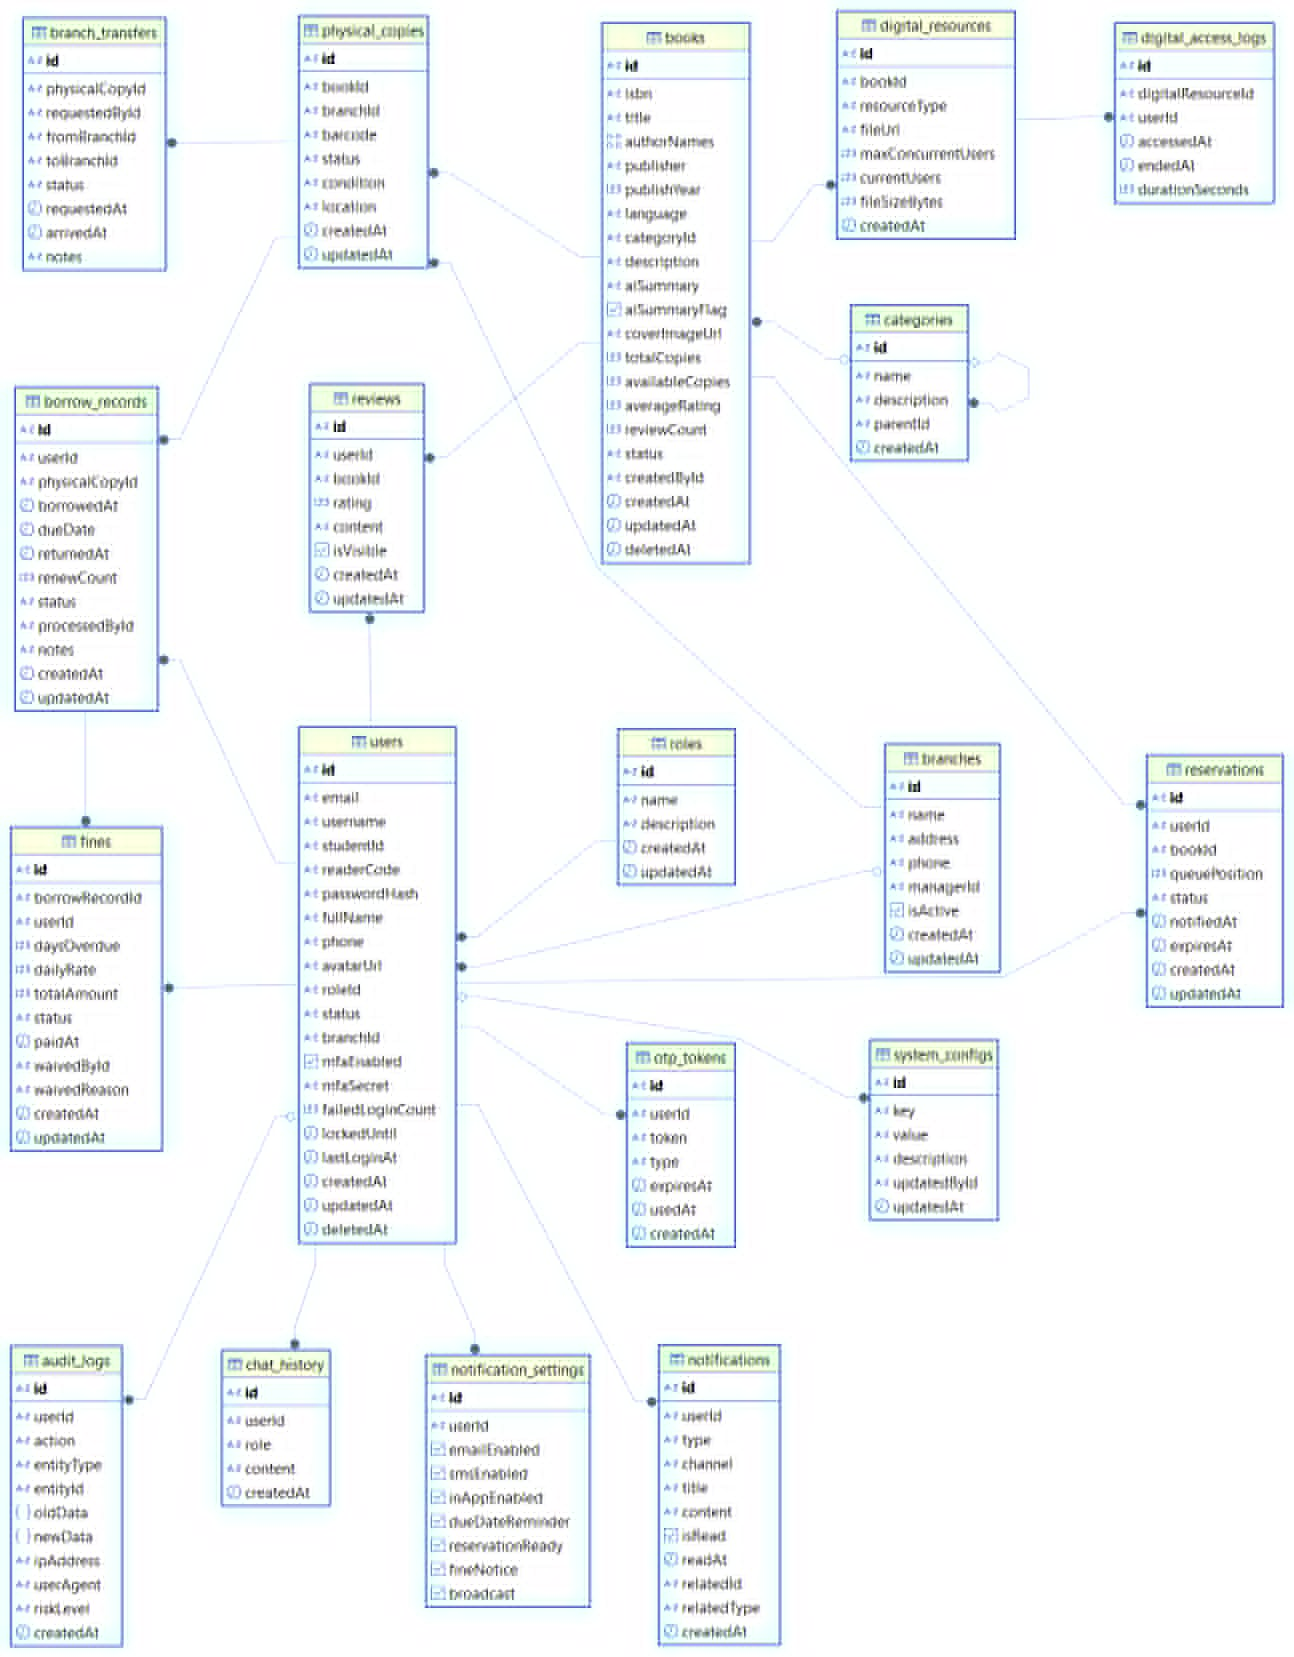
\includegraphics[width=0.6\linewidth]{Images/db.jpg}
	\vspace{10pt}
	\caption{Lược đồ Cơ sở Dữ liệu Quan hệ của Hệ thống Quản lý Thư viện Trực tuyến}
	\label{fig:database_account}
\end{figure}
Lược đồ trên đại diện cho cấu trúc quan hệ được triển khai trên PostgreSQL.

Tài khoản người dùng được tập trung trong bảng \texttt{users}, liên kết với \texttt{roles} qua khóa ngoại \texttt{roleId} để kiểm tra quyền RBAC. Các cờ an ninh như \texttt{status}, \texttt{failedLoginCount}, và \texttt{lockedUntil} thực thi các ràng buộc an ninh đăng nhập.

Các bảng còn lại ánh xạ trực tiếp tới các định nghĩa thực thể và quan hệ EERD đã mô tả ở trên.

\subsection{Sơ đồ Lớp (Class Diagram)}

\subsubsection{Quản lý Tài khoản và Truy cập}

\begin{figure}[H]
	\centering
	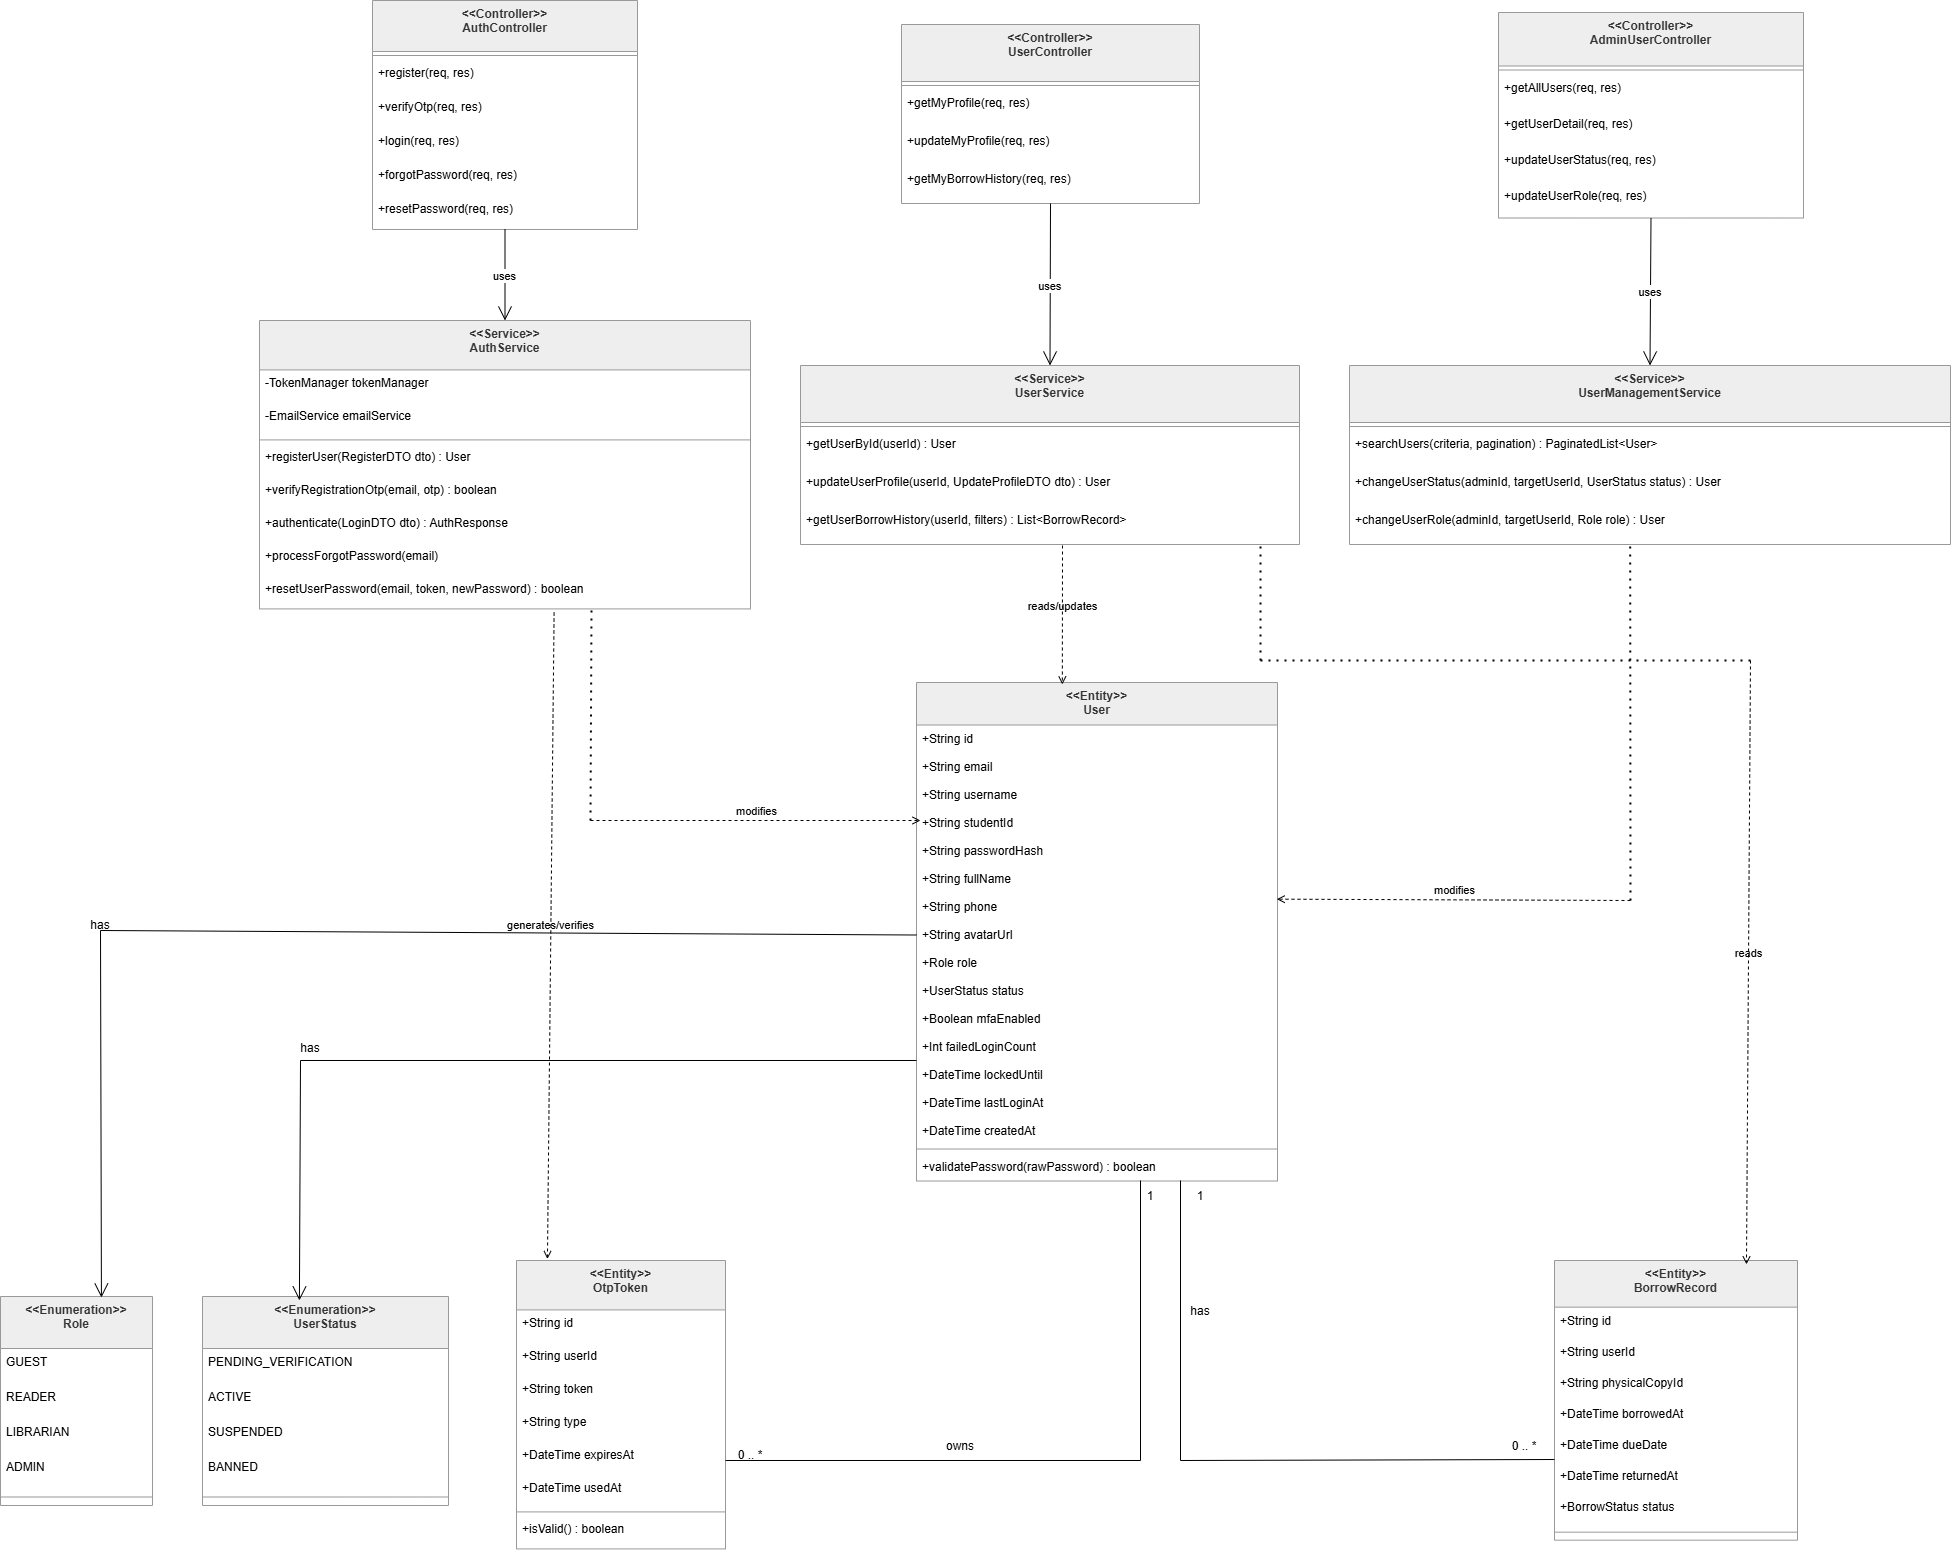
\includegraphics[width=0.6\linewidth]{Images/quanlytruycapvataikhoan.png}
	\vspace{10pt}
	\caption{Sơ đồ Lớp cho Quản lý Tài khoản và Truy cập}
	\label{fig:class_account}
\end{figure}

Sơ đồ lớp \textbf{Quản lý Tài khoản và Truy cập} mô hình hóa cấu trúc đối tượng, thuộc tính và phương thức cho xác thực và quản lý hồ sơ.

Thực thể trung tâm là \texttt{User}, chứa các thuộc tính \texttt{id}, \texttt{email}, \texttt{username}, \texttt{fullName}, \texttt{phone}, \texttt{avatarUrl}, \texttt{studentId}, cùng các thuộc tính an ninh \texttt{passwordHash}, \texttt{mfaEnabled}, \texttt{failedLoginCount}, \texttt{lockedUntil}, \texttt{lastLoginAt} và \texttt{createdAt}. Phương thức cốt lõi \texttt{validatePassword(rawPassword)} thực hiện xác minh thông tin đăng nhập.

\texttt{User} liên kết với \texttt{Role} (GUEST, READER, LIBRARIAN, ADMIN) và \texttt{UserStatus} (PENDING\_VERIFICATION, ACTIVE, SUSPENDED, BANNED). \texttt{User} liên kết $1 - 0..*$ với \texttt{OtpToken} (phương thức \texttt{isValid()}) và $1 - 0..*$ với \texttt{BorrowRecord}.

Về mặt kiến trúc, \texttt{AuthController} phụ thuộc vào \texttt{AuthService} (\texttt{registerUser}, \texttt{verifyRegistrationOtp}, \texttt{authenticate}, \texttt{processForgotPassword}, \texttt{resetPasswordUser}). \texttt{UserController} phụ thuộc vào \texttt{UserService} (\texttt{getUserById}, \texttt{updateUserProfile}, \texttt{getUserBorrowHistory}). \texttt{AdminUserController} sử dụng \texttt{UserManagementService} (\texttt{searchUsers}, \texttt{getUserDetail}, \texttt{changeUserStatus}, \texttt{changeUserRole}).

\subsubsection{Quản lý Danh mục Sách}

\begin{figure}[H]
	\centering
	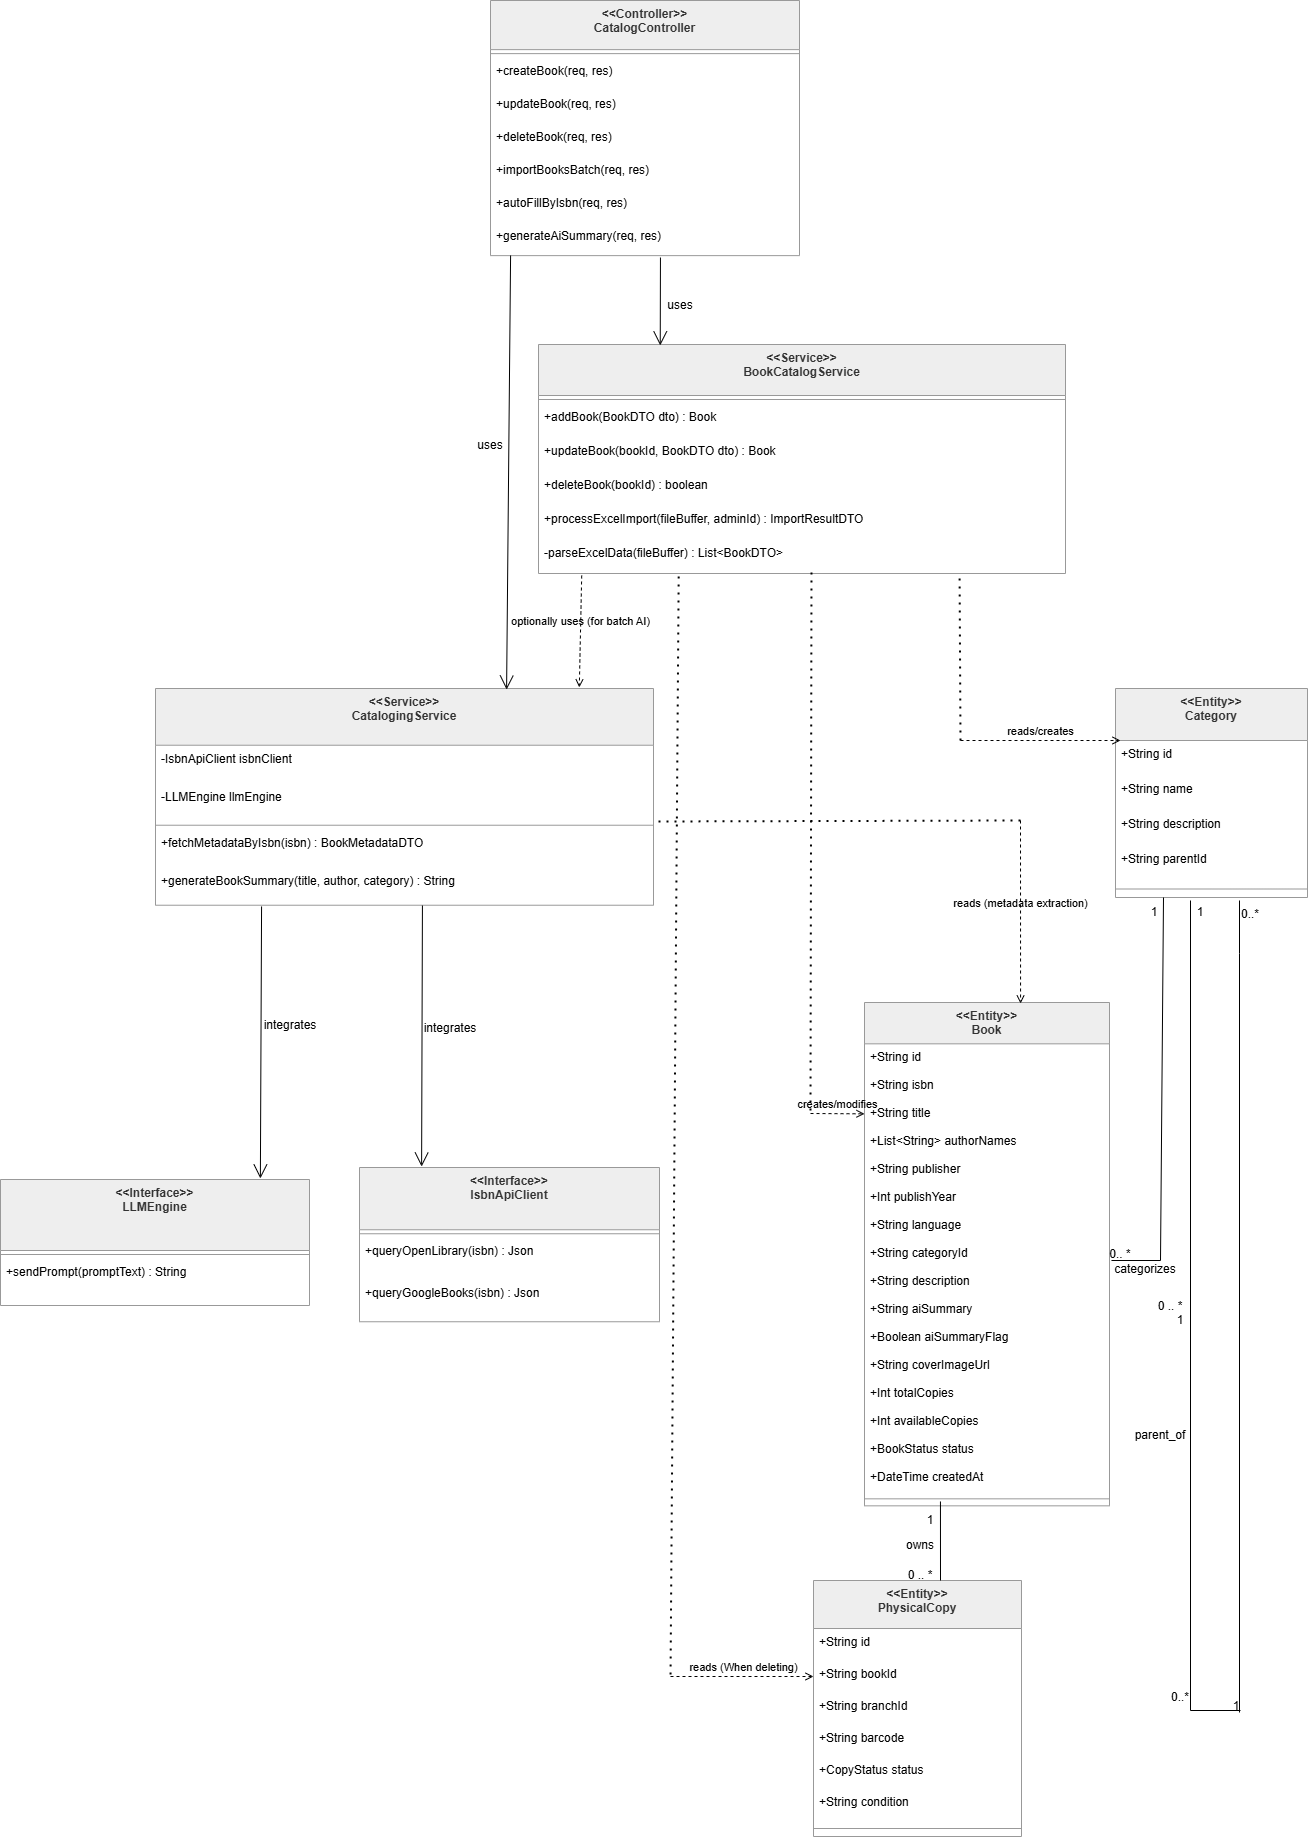
\includegraphics[width=0.6\linewidth]{Images/quanlydanhmuc.png}
	\vspace{10pt}
	\caption{Sơ đồ Lớp cho Quản lý Danh mục Sách}
	\label{fig:class_catalog}
\end{figure}

Các cấu trúc dữ liệu cốt lõi bao gồm \texttt{Category}, \texttt{Book} và \texttt{PhysicalCopy}. \texttt{Category} sở hữu phân cấp tự tham chiếu ($1 \to 0..\ast$) qua \texttt{parentId} và liên kết $1 \to 0..\ast$ với \texttt{Book}.

\texttt{Book} chứa dữ liệu tả danh mục (\texttt{isbn}, \texttt{title}, \texttt{authorNames}, \texttt{publisher}, \texttt{publishYear}, \texttt{language}, \texttt{totalCopies}, \texttt{availableCopies}, \texttt{aiSummary}) và liên kết $1 \to 0..\ast$ với \texttt{PhysicalCopy} (\texttt{barcode}, \texttt{CopyStatus status}, \texttt{condition}).

\texttt{CatalogController} ủy quyền cho \texttt{BookCatalogService} (\texttt{addBook}, \texttt{updateBook}, \texttt{deleteBook}, \texttt{autoFillByIsbn}, \texttt{generateAiSummary}, \texttt{processExcelImport}). \texttt{BookCatalogService} tương tác với \texttt{CatalogingService}, lớp bọc \texttt{IsbnApiClient} (\texttt{queryOpenLibrary}, \texttt{queryGoogleBooks}) và \texttt{LLMEngine} (\texttt{generateBookSummary}) cho biên mục tự động.

\subsubsection{Quản lý Lưu thông Tài liệu}

\begin{figure}[H]
	\centering
	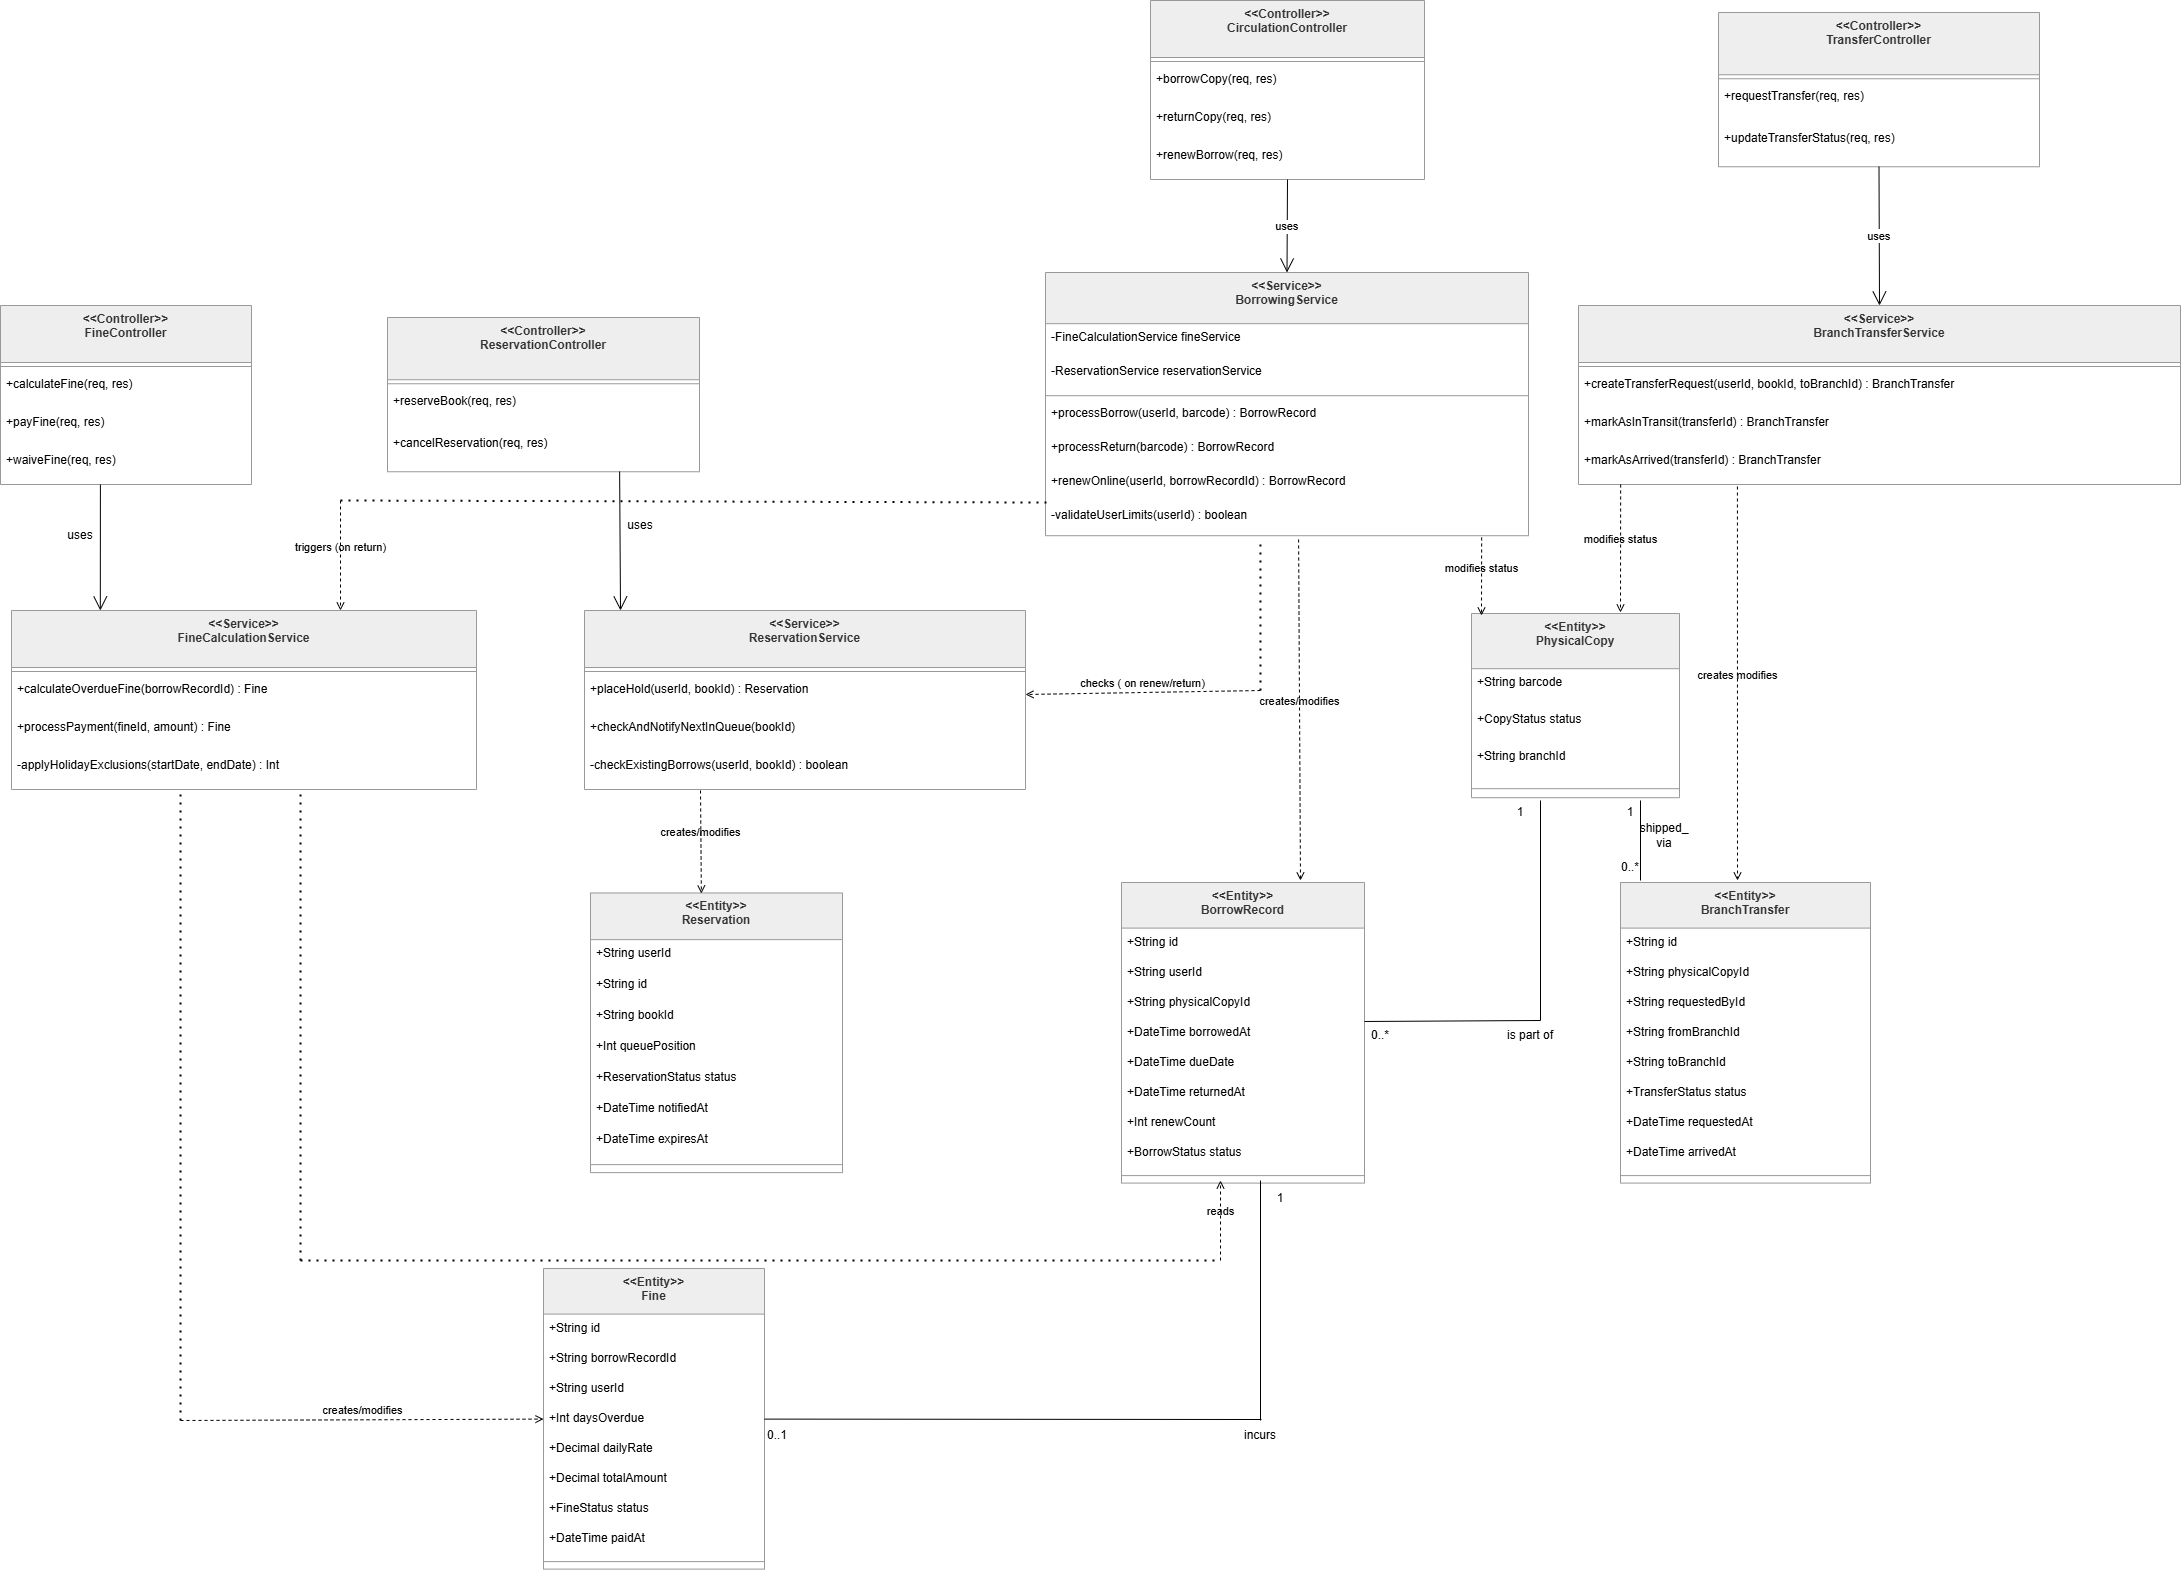
\includegraphics[width=0.6\linewidth]{Images/quanlyluuthong.png}
	\vspace{10pt}
	\caption{Sơ đồ Lớp cho Quản lý Lưu thông Tài liệu}
	\label{fig:class_circulation}
\end{figure}

Thực thể trung tâm \texttt{BorrowRecord} (\texttt{borrowedAt}, \texttt{dueDate}, \texttt{returnedAt}, \texttt{renewCount}, \texttt{BorrowStatus status}) liên kết với \texttt{PhysicalCopy} ($1 - 0..*$). \texttt{Reservation} (\texttt{queuePosition}, \texttt{ReservationStatus status}) và \texttt{Fine} ($1 - 0..1$ với \texttt{BorrowRecord}) xử lý hàng chờ đặt chỗ và tính phạt. \texttt{BranchTransfer} theo dõi việc chuyển sách giữa các chi nhánh.

\texttt{CirculationController} sử dụng \texttt{BorrowingService} (\texttt{processBorrow}, \texttt{processReturn}, \texttt{renewOnline}). \texttt{ReservationController} sử dụng \texttt{ReservationService} (\texttt{placeHold}, \texttt{cancelReservation}). \texttt{FineController} sử dụng \texttt{FineCalculationService} (\texttt{calculateOverdueFine}, \texttt{processPayment}). \texttt{TransferController} sử dụng \texttt{BranchTransferService} (\texttt{createTransferRequest}, \texttt{markInTransit}, \texttt{markAsArrived}).

\subsubsection{Tìm kiếm và Khai thác Tài nguyên}

\begin{figure}[H]
	\centering
	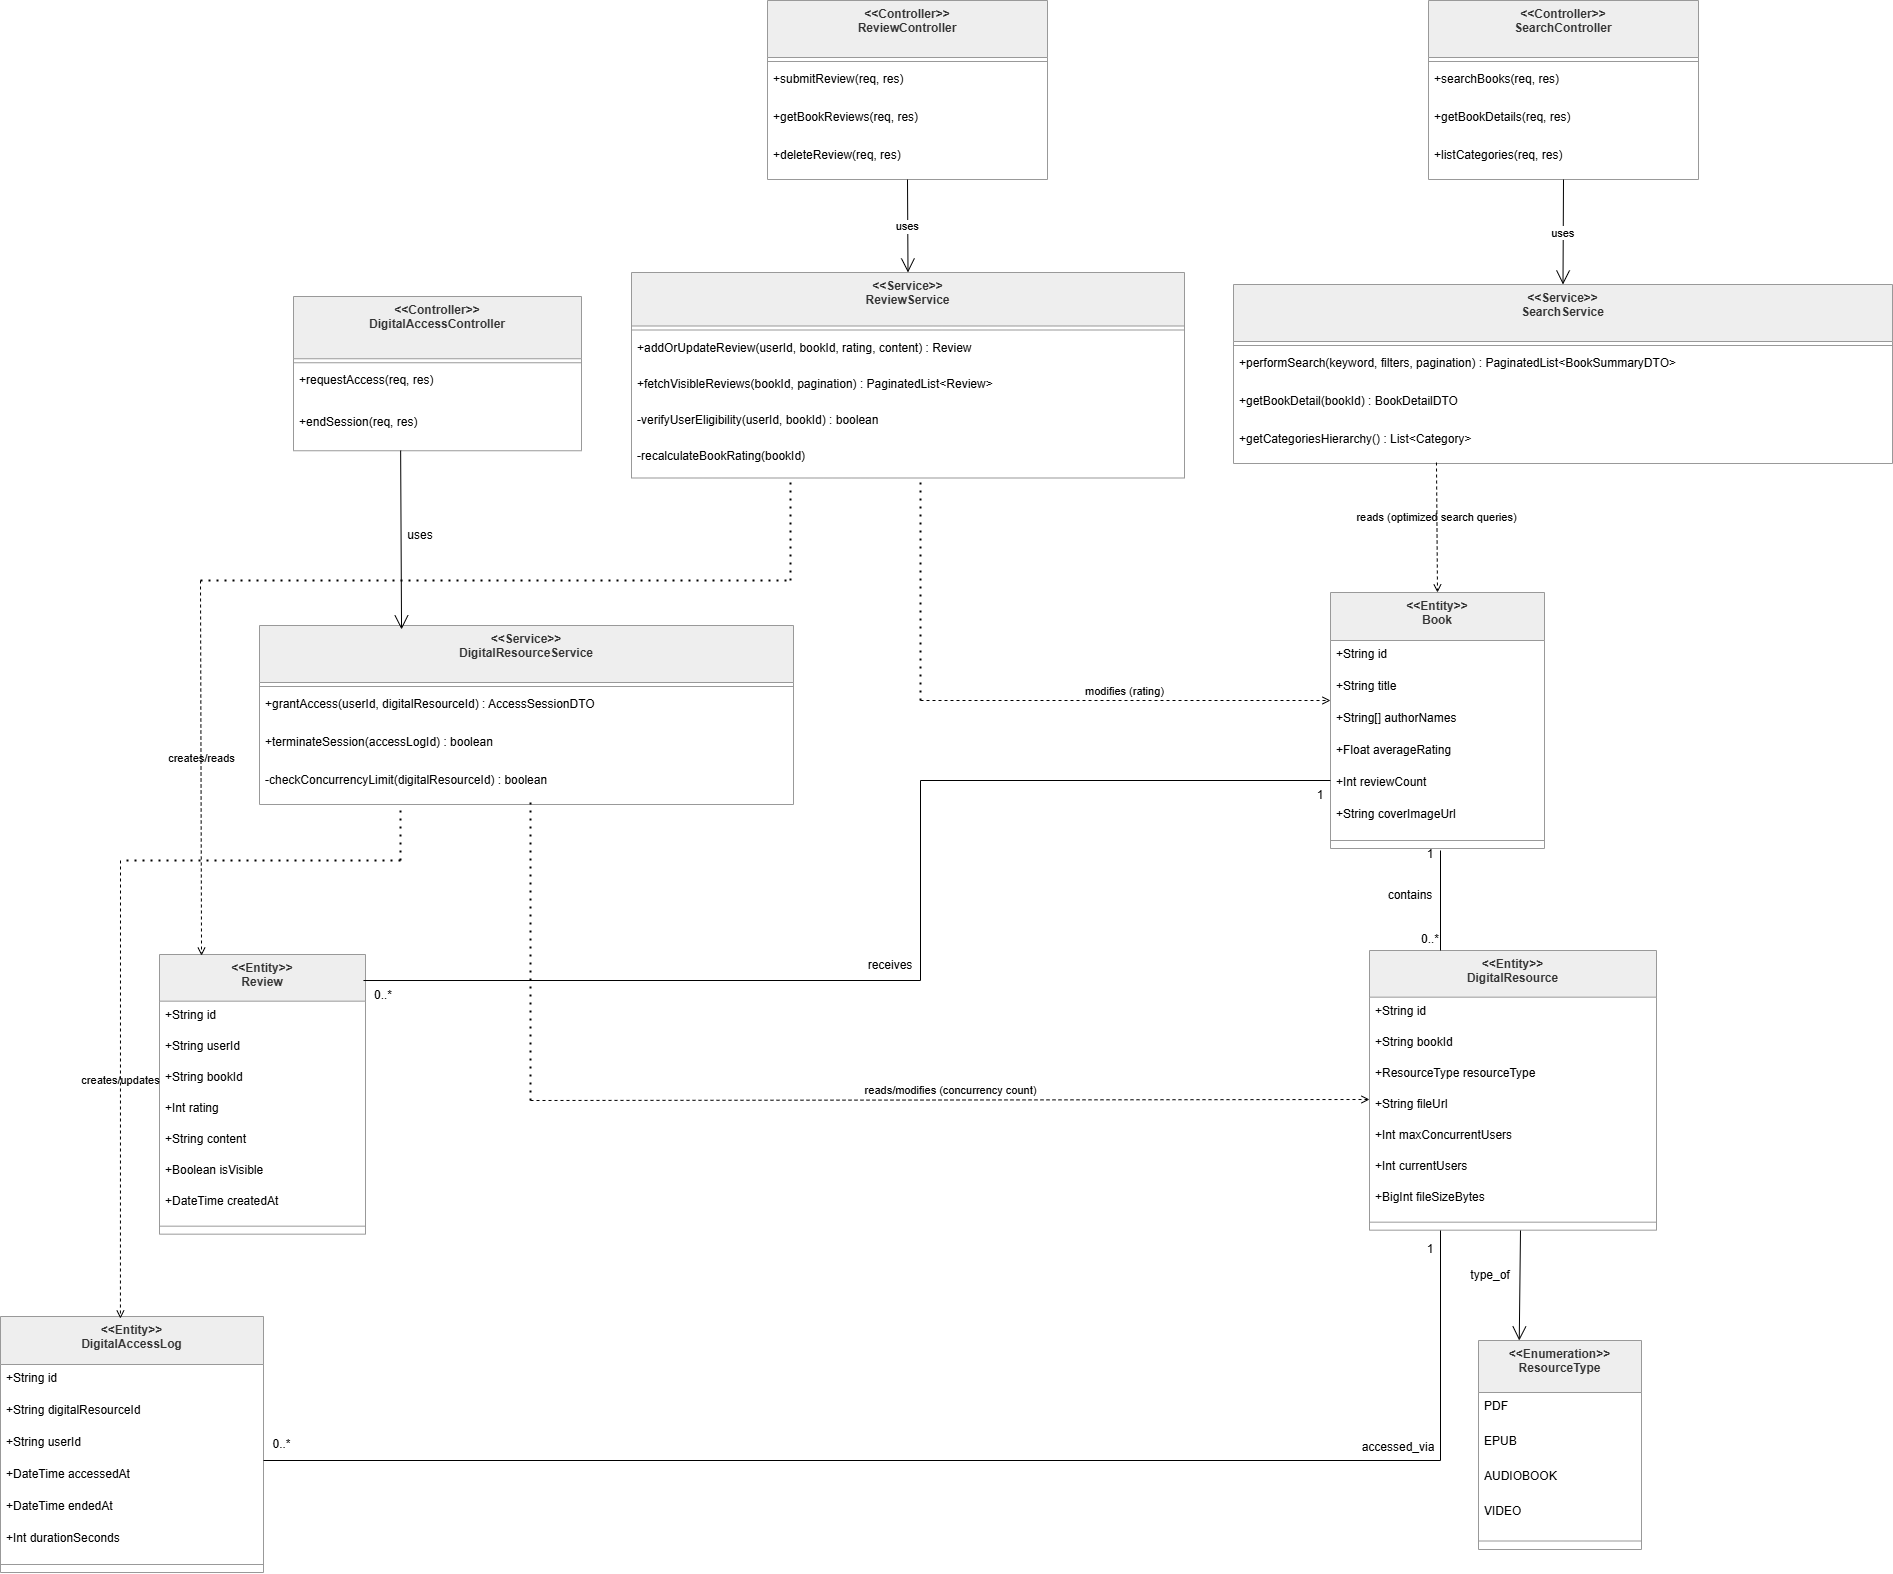
\includegraphics[width=0.6\linewidth]{Images/truycapvakhaithactainguyen.png}
	\vspace{10pt}
	\caption{Sơ đồ Lớp cho Tìm kiếm và Khai thác Tài nguyên}
	\label{fig:class_exploration}
\end{figure}

\texttt{Book} liên kết $1 - 0..*$ với \texttt{Review} ($0..* - 1$ với \texttt{Book}) lưu trữ đánh giá của người dùng.

\texttt{SearchController} sử dụng \texttt{SearchService} (\texttt{performSearch}, \texttt{getBookDetail}). \texttt{ReviewController} sử dụng \texttt{ReviewService} (\texttt{addOrUpdateReview}, \texttt{recalculateBookRating}).

\subsubsection{Trợ lý Ảo AI và Gợi ý}

\begin{figure}[H]
	\centering
	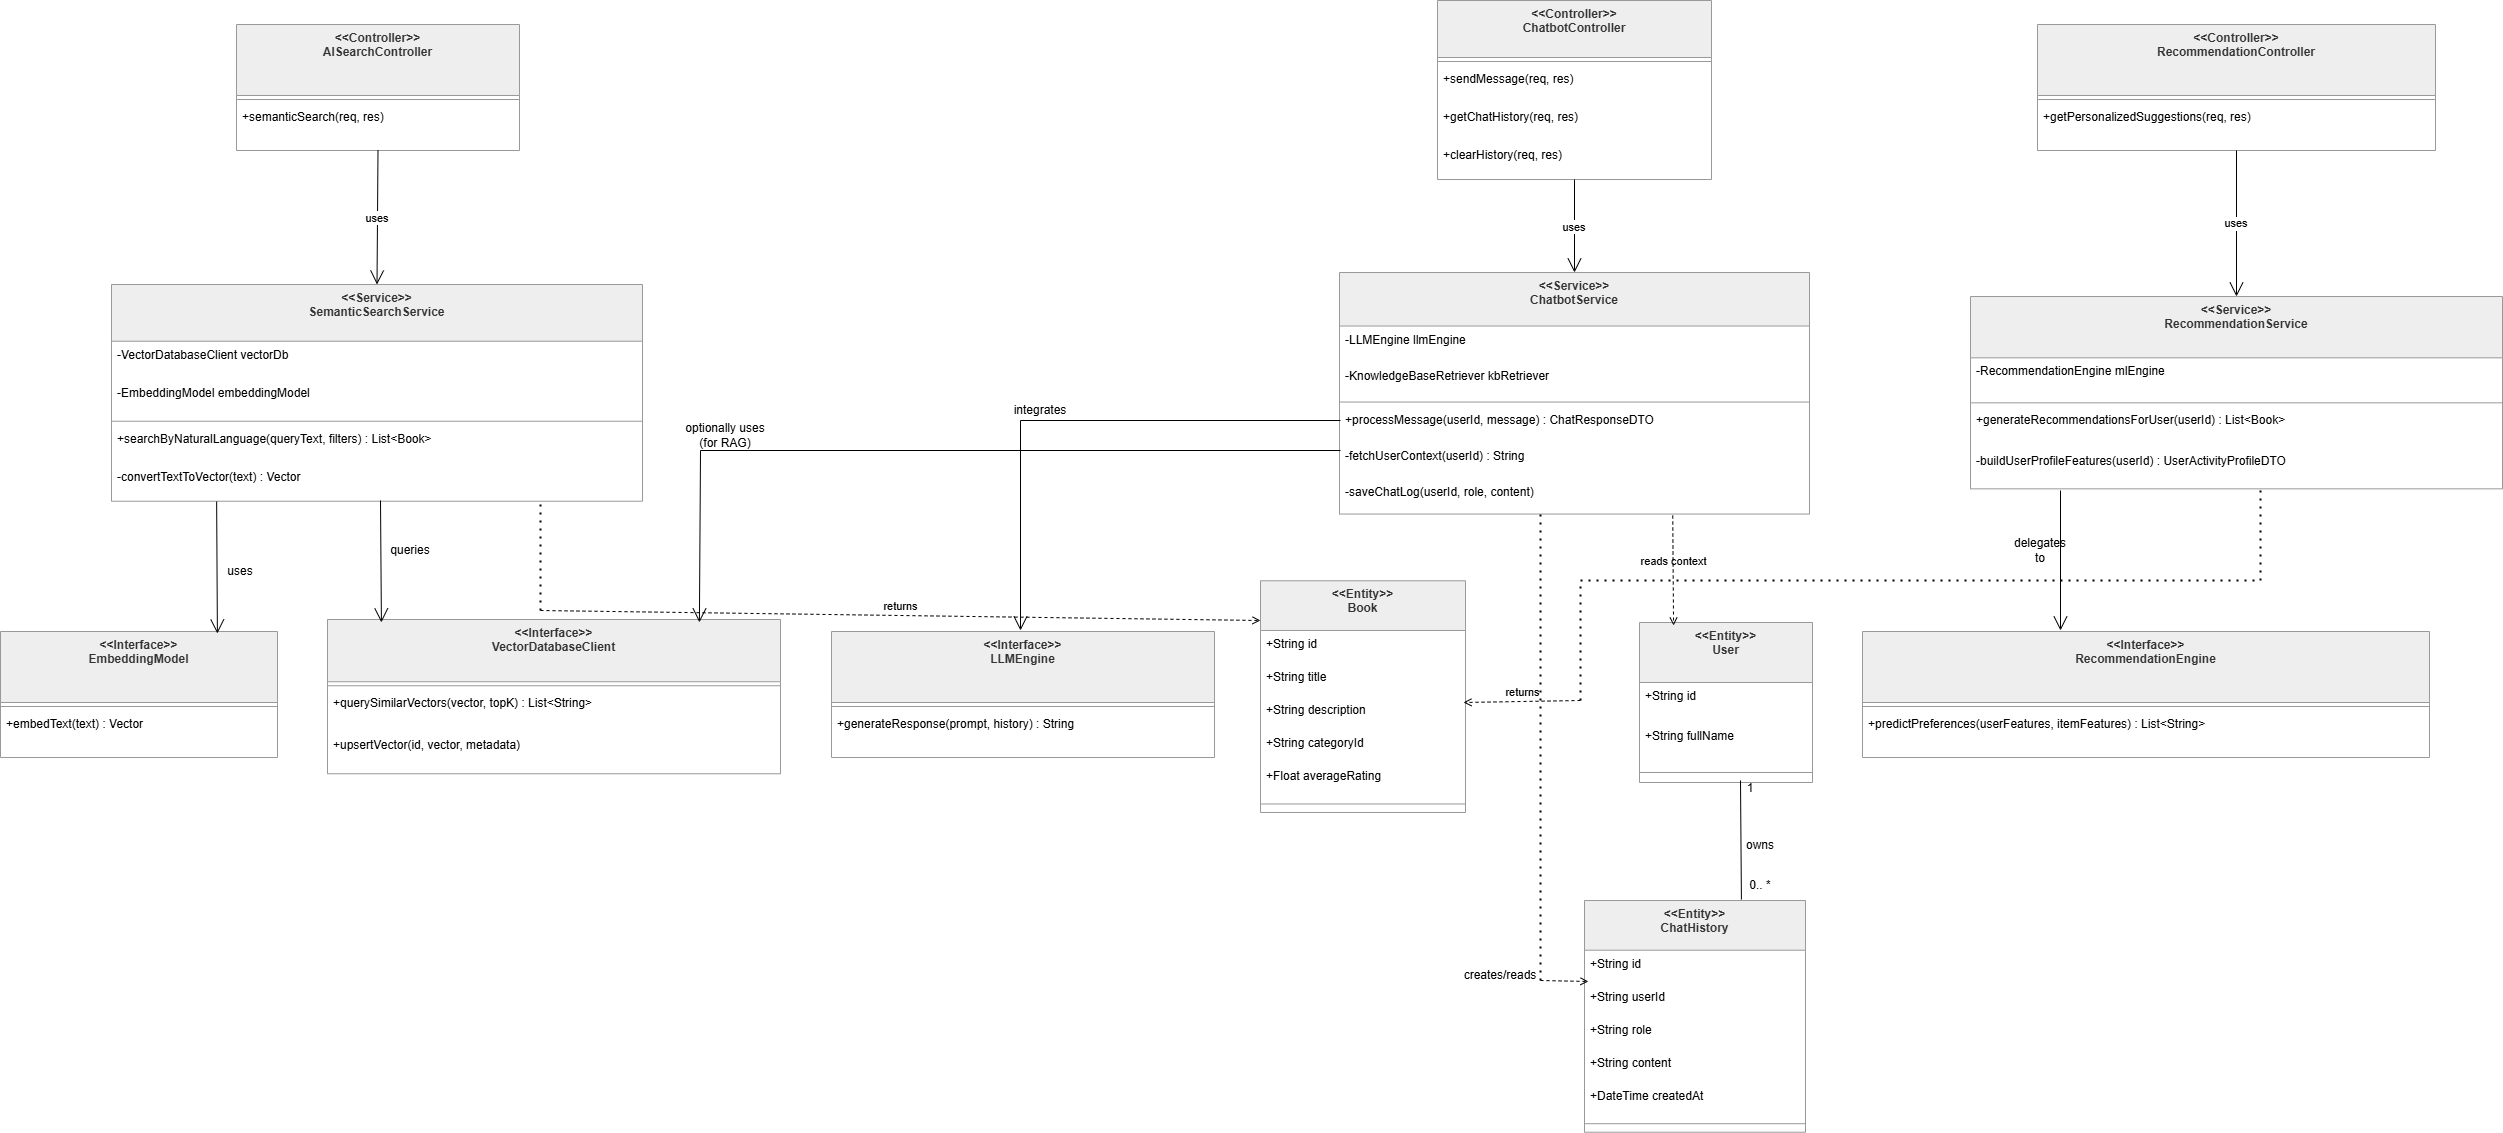
\includegraphics[width=0.6\linewidth]{Images/AI.png}
	\vspace{10pt}
	\caption{Sơ đồ Lớp cho Trợ lý Ảo AI và Gợi ý}
	\label{fig:class_ai}
\end{figure}

\texttt{AISearchController} sử dụng \texttt{SemanticSearchService} (\texttt{searchByNaturalLanguage}) giao tiếp với \texttt{EmbeddingModel} và \texttt{VectorDatabaseClient}.

\texttt{ChatbotController} sử dụng \texttt{ChatbotService} (\texttt{sendMessage}, \texttt{getChatHistory}), giao tiếp với \texttt{LLMEngine} và \texttt{VectorDatabaseClient} (ngữ cảnh RAG), ghi nhật ký hội thoại trong \texttt{ChatHistory}.

\texttt{RecommendationController} sử dụng \texttt{RecommendationService} (\texttt{getPersonalizedSuggestions}), tận dụng \texttt{RecommendationEngine} (\texttt{predictPreferences}) để trả về danh sách sách gợi ý phù hợp.

\subsubsection{Thông báo và Tương tác}

\begin{figure}[H]
	\centering
	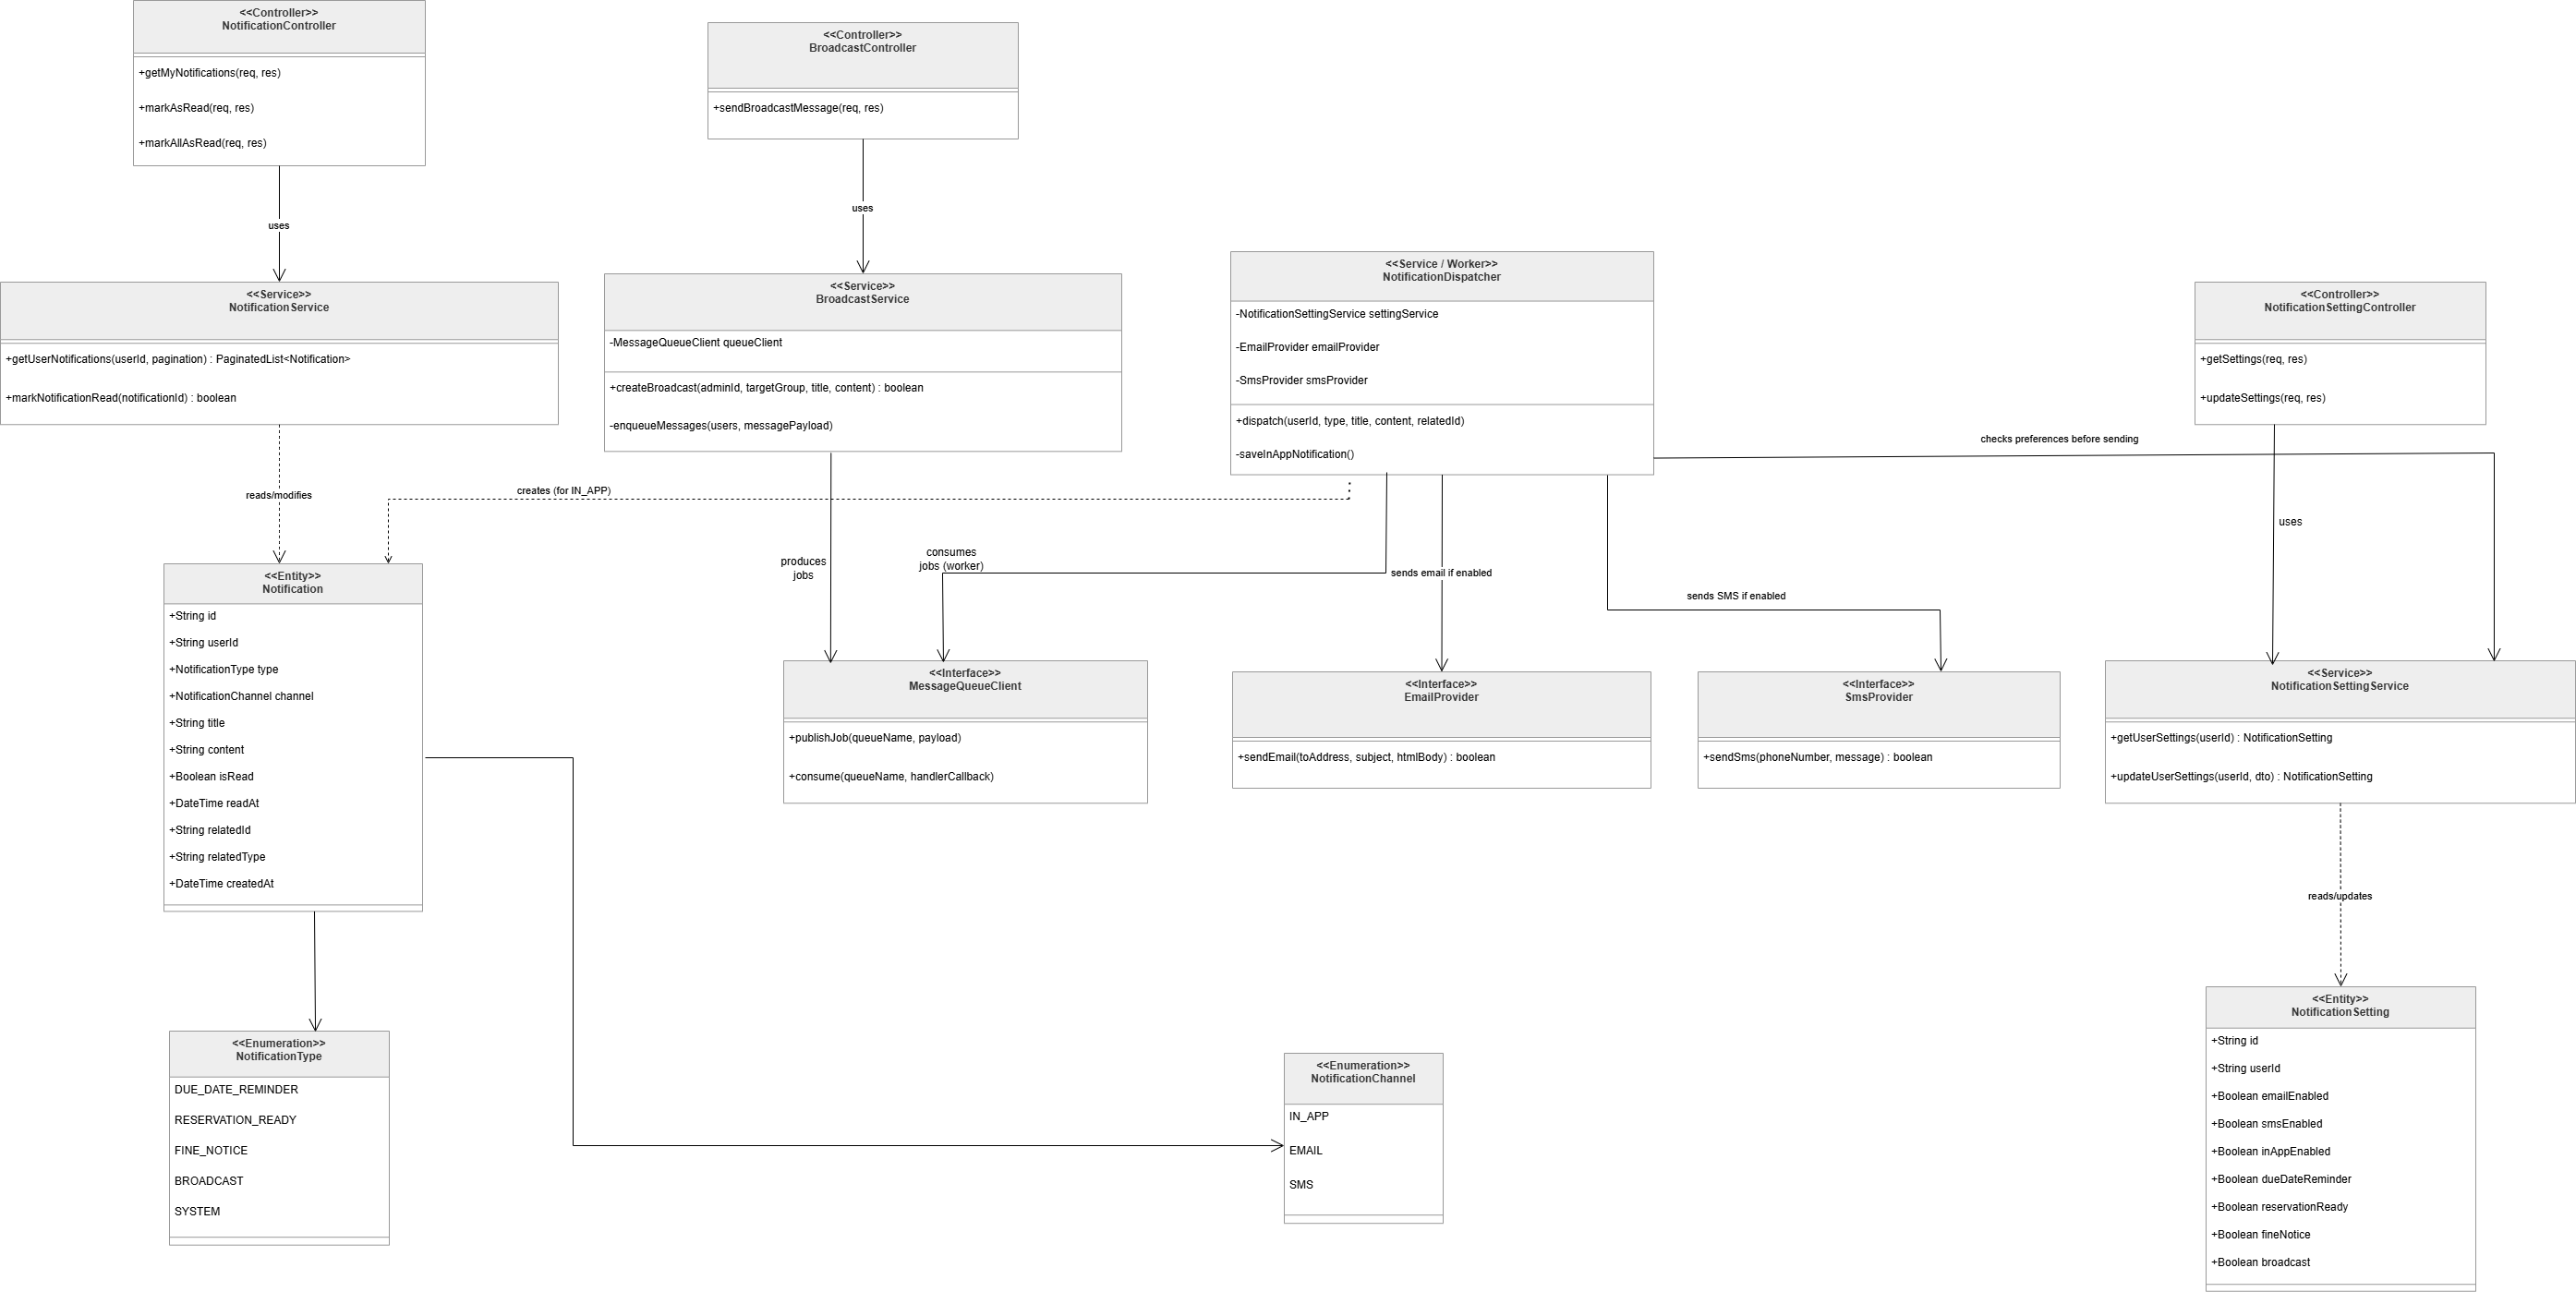
\includegraphics[width=0.6\linewidth]{Images/thongbao.png}
	\vspace{10pt}
	\caption{Sơ đồ Lớp cho Thông báo và Tương tác}
	\label{fig:class_notification}
\end{figure}

Các thực thể bao gồm \texttt{Notification} (\texttt{isRead}, \texttt{NotificationType}, \texttt{NotificationChannel}) và \texttt{NotificationSetting} (\texttt{emailEnabled}, \texttt{smsEnabled}, \texttt{inAppEnabled}).

\texttt{NotificationSettingController} sử dụng \texttt{NotificationSettingService}. \texttt{NotificationController} sử dụng \texttt{NotificationService}. \texttt{BroadcastController} sử dụng \texttt{BroadcastService} đẩy các tác vụ vào \texttt{MessageQueueClient}. Tiến trình chạy ngầm bất đồng bộ \texttt{NotificationDispatcher} xử lý các tác vụ trong hàng chờ và gửi cảnh báo qua \texttt{EmailProvider} và \texttt{SmsProvider}.

\subsubsection{Quản trị Hệ thống}

\begin{figure}[H]
	\centering
	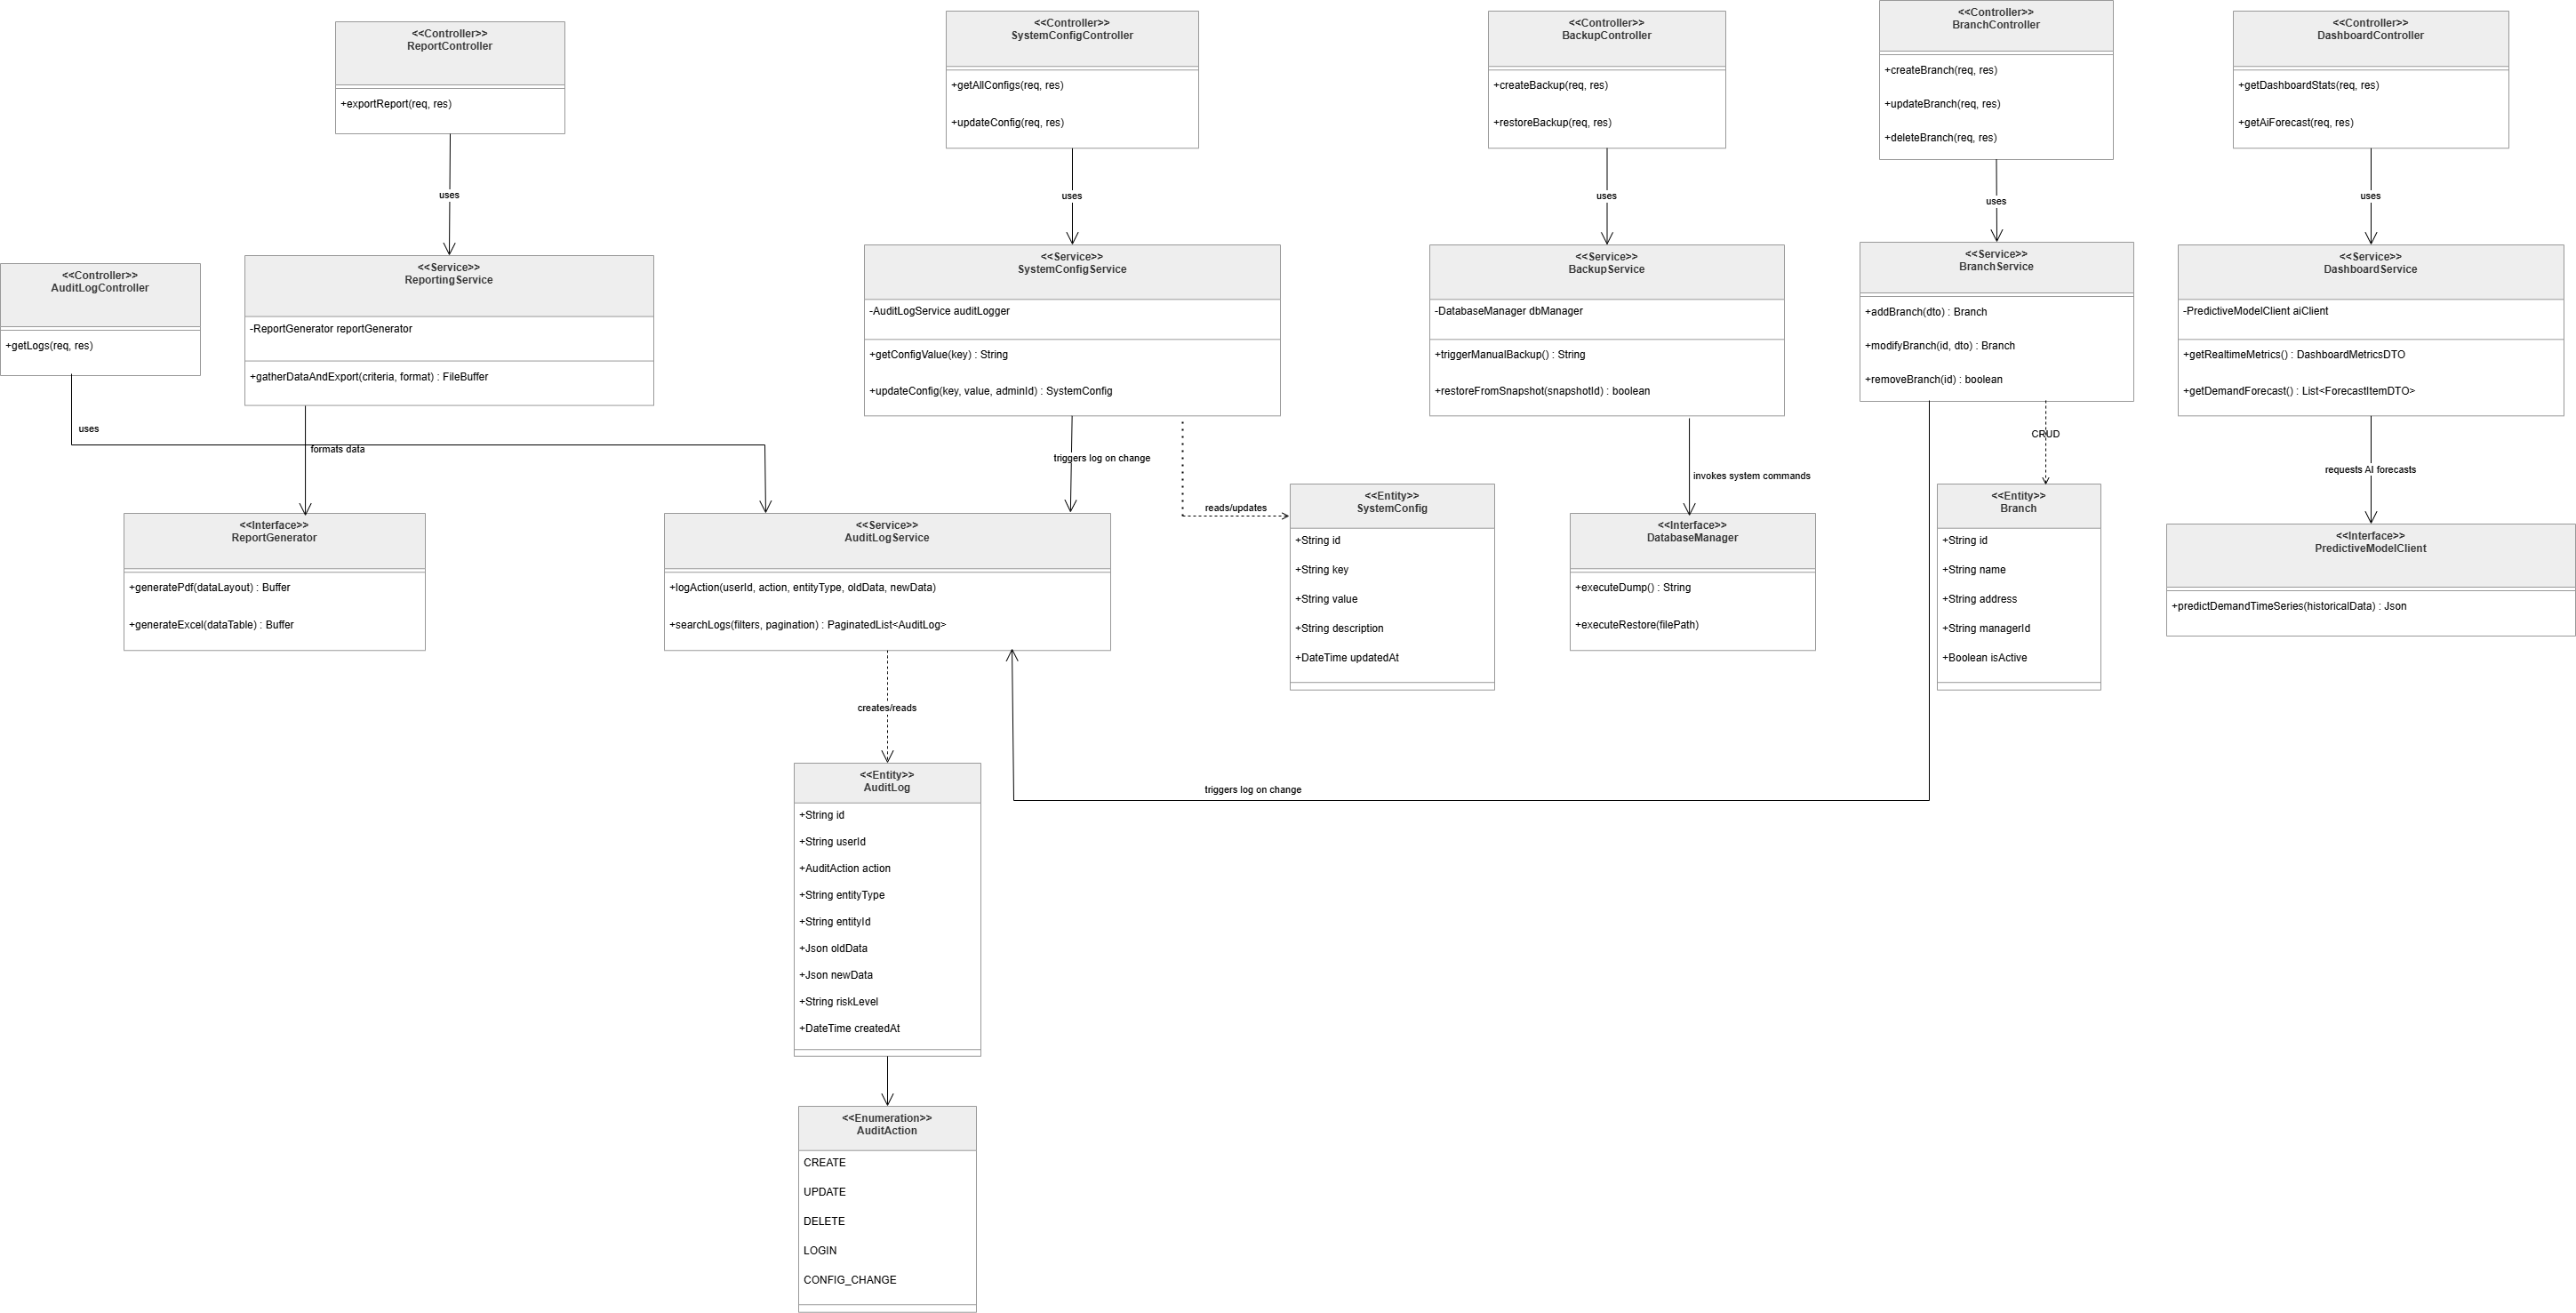
\includegraphics[width=0.6\linewidth]{Images/baocaovaquantri.png}
	\vspace{10pt}
	\caption{Sơ đồ Lớp cho Quản trị Hệ thống}
	\label{fig:class_admin}
\end{figure}

Các thực thể cốt lõi: \texttt{AuditLog} (\texttt{action}, \texttt{oldData}, \texttt{newData}, \texttt{riskLevel}), \texttt{SystemConfig} (\texttt{key}, \texttt{value}) và \texttt{Branch} (\texttt{name}, \texttt{address}, \texttt{isActive}).

\texttt{AuditLogController} sử dụng \texttt{AuditLogService}. \texttt{ReportController} sử dụng \texttt{ReportingService} (\texttt{ReportGenerator}). \texttt{SystemConfigController} sử dụng \texttt{SystemConfigService}. \texttt{BackupController} sử dụng \texttt{BackupService} (\texttt{DatabaseManager}). \texttt{BranchController} sử dụng \texttt{BranchService}. \texttt{DashboardController} sử dụng \texttt{DashboardService} giao tiếp với \texttt{PredictiveModelClient} cho dự báo nhu cầu.

\subsection{Sơ đồ Hoạt động (Activity Diagrams)}
\subsubsection{Đăng ký Tài khoản}

\begin{figure}[H]
	\centering
	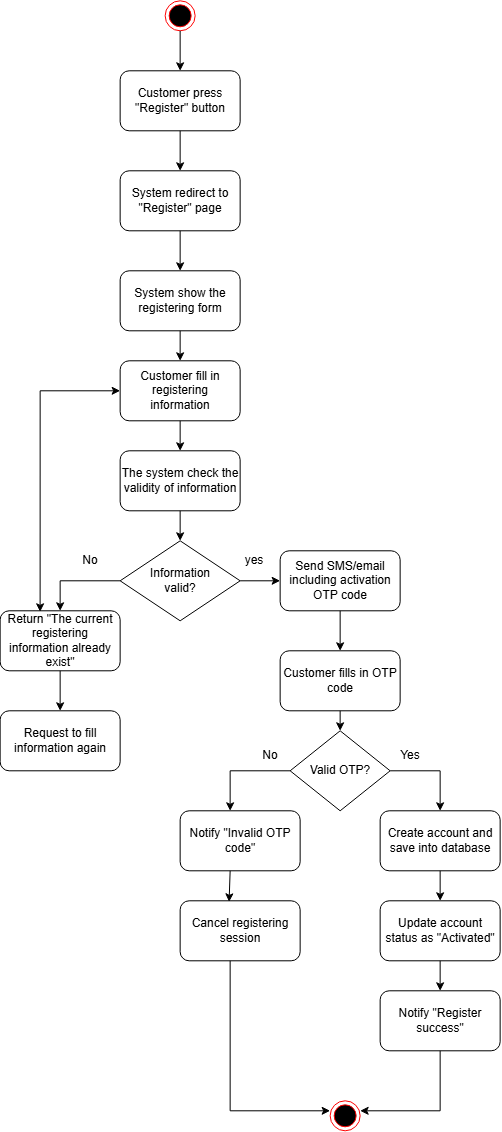
\includegraphics[width=0.6\linewidth]{Images/dangki.png}
	\vspace{10pt}
	\caption{Sơ đồ Hoạt động cho Đăng ký Tài khoản}
	\label{fig:activity_register}
\end{figure}

\begin{enumerate}
	\item Khách truy cập trang đăng ký tài khoản.
	\item Hệ thống hiển thị biểu mẫu đăng ký.
	\item Khách nhập các thông tin (Họ tên, Email/Số điện thoại, Mật khẩu).
	\item Hệ thống kiểm tra cú pháp dữ liệu đầu vào.
	\item Hệ thống kiểm tra xem Email/Số điện thoại đã tồn tại trong cơ sở dữ liệu chưa.
	\item \textbf{Nhánh Hợp lệ:}
	      \begin{itemize}
		      \item Nếu hợp lệ, hệ thống gửi Email/SMS chứa mã OTP hoặc liên kết kích hoạt.
		      \item Khách nhập mã OTP hoặc nhấn liên kết kích hoạt.
		      \item Hệ thống xác thực mã OTP hoặc token liên kết.
		      \item Nếu OTP/liên kết hợp lệ: Hệ thống tạo tài khoản người dùng, lưu vào DB, chuyển trạng thái sang "Đã kích hoạt" và báo thành công.
	      \end{itemize}
	\item \textbf{Nhánh Không Hợp lệ:}
	      \begin{itemize}
		      \item Nếu dữ liệu không hợp lệ hoặc Email/Số điện thoại đã tồn tại: Hệ thống hiển thị thông báo lỗi và yêu cầu nhập lại.
		      \item Nếu OTP không hợp lệ: Hệ thống hiển thị lỗi sai OTP và hủy phiên đăng ký.
	      \end{itemize}
\end{enumerate}

\subsubsection{Đăng nhập Hệ thống}

\begin{figure}[H]
	\centering
	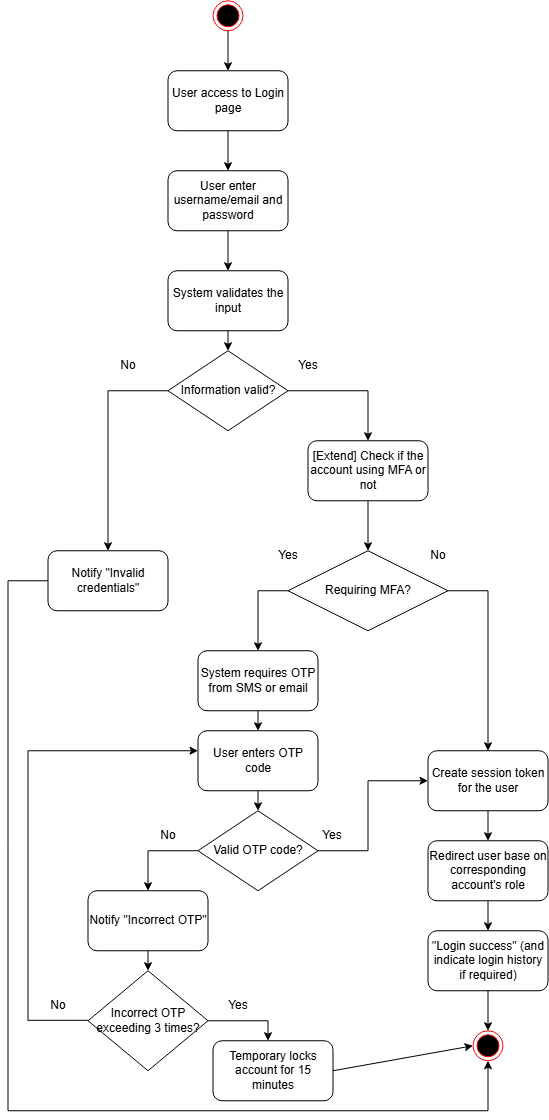
\includegraphics[width=0.6\linewidth]{Images/dangnhap.png}
	\vspace{10pt}
	\caption{Sơ đồ Hoạt động cho Đăng nhập Hệ thống}
	\label{fig:activity_login}
\end{figure}

\begin{enumerate}
	\item Người dùng truy cập giao diện đăng nhập.
	\item Người dùng nhập Email/Tên đăng nhập và Mật khẩu.
	\item Hệ thống xác thực thông tin đăng nhập với DB.
	\item Nếu thông tin không chính xác: Hệ thống hiển thị lỗi "Tài khoản hoặc mật khẩu không đúng".
	\item Nếu thông tin chính xác: Hệ thống kiểm tra xem có yêu cầu Xác thực Nhiều yếu tố (MFA) hay không.
	\item Nếu bật MFA: Hệ thống yêu cầu mã OTP; người dùng nhập OTP; hệ thống xác thực mã.
	\item Nếu OTP sai: Hiển thị lỗi "Mã OTP không chính xác". Nếu nhập sai quá 3 lần, tài khoản bị tạm khóa trong 15 phút.
	\item Nếu OTP đúng (hoặc không yêu cầu MFA): Khởi tạo phiên/token, chuyển hướng người dùng đến bảng điều khiển theo vai trò và hiển thị thông báo thành công.
\end{enumerate}

\subsubsection{Đặt lại Mật khẩu}

\begin{figure}[H]
	\centering
	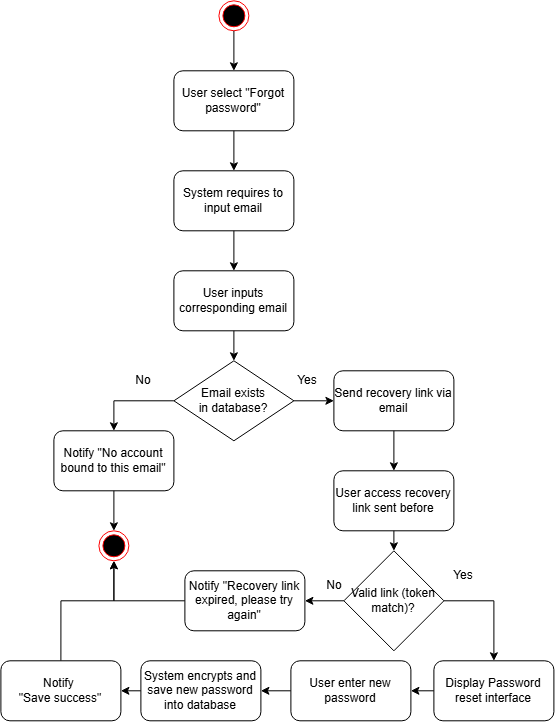
\includegraphics[width=0.6\linewidth]{Images/datlai.png}
	\vspace{10pt}
	\caption{Sơ đồ Hoạt động cho Đặt lại Mật khẩu}
	\label{fig:activity_reset_password}
\end{figure}

\begin{enumerate}
	\item Người dùng chọn "Quên mật khẩu".
	\item Hệ thống yêu cầu nhập Email.
	\item Người dùng gửi Email.
	\item Hệ thống xác minh sự tồn tại của Email. Nếu không tìm thấy: Hiển thị "Không tìm thấy tài khoản với email này".
	\item Nếu tìm thấy: Hệ thống gửi liên kết đặt lại qua Email. Người dùng mở liên kết; hệ thống kiểm tra tính hợp lệ của token.
	\item Nếu liên kết hết hạn/không hợp lệ: Hiển thị "Liên kết đặt lại đã hết hạn" và yêu cầu thực hiện lại.
	\item Nếu liên kết hợp lệ: Hiển thị biểu mẫu đặt lại; người dùng nhập mật khẩu mới; hệ thống băm và cập nhật mật khẩu, thông báo thành công.
\end{enumerate}

\subsubsection{Xem Lịch sử Mượn/Trả}

\begin{figure}[H]
	\centering
	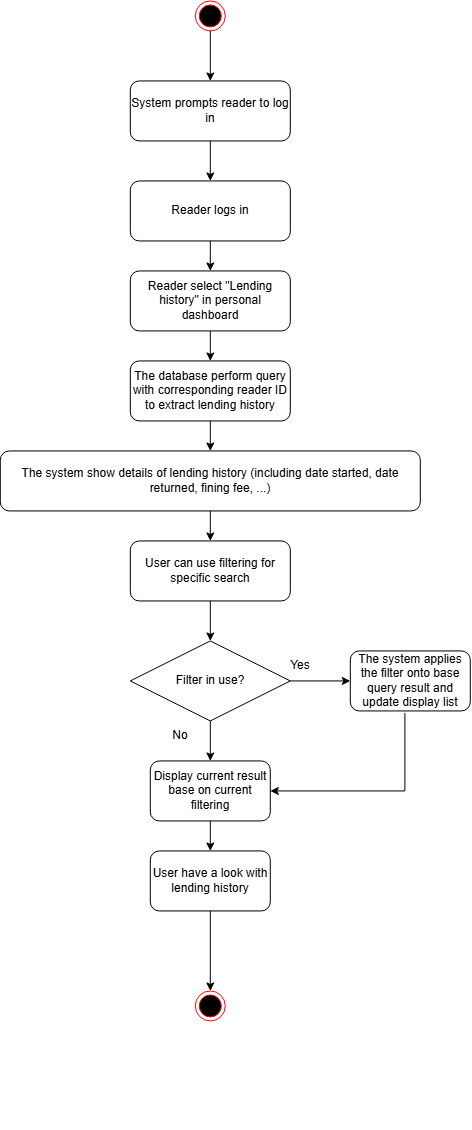
\includegraphics[width=0.6\linewidth]{Images/xemlichsu.png}
	\vspace{10pt}
	\caption{Sơ đồ Hoạt động cho Xem Lịch sử Mượn/Trả}
	\label{fig:activity_view_history}
\end{figure}

\begin{enumerate}
	\item Người dùng đăng nhập vào hệ thống.
	\item Người dùng mở "Lịch sử Mượn trả" trên bảng điều khiển.
	\item Hệ thống truy vấn DB lấy các bản ghi mượn khớp với ID Người dùng.
	\item Hệ thống hiển thị bảng lịch sử mượn (Tên sách, Ngày mượn, Hạn trả, Ngày trả, Trạng thái, Tiền phạt).
	\item Người dùng có thể áp dụng bộ lọc theo khoảng thời gian hoặc trạng thái.
	\item Hệ thống làm mới bảng hiển thị dựa trên tham số lọc.
\end{enumerate}

\subsubsection{Quản lý Tài khoản Người dùng}

\begin{figure}[H]
	\centering
	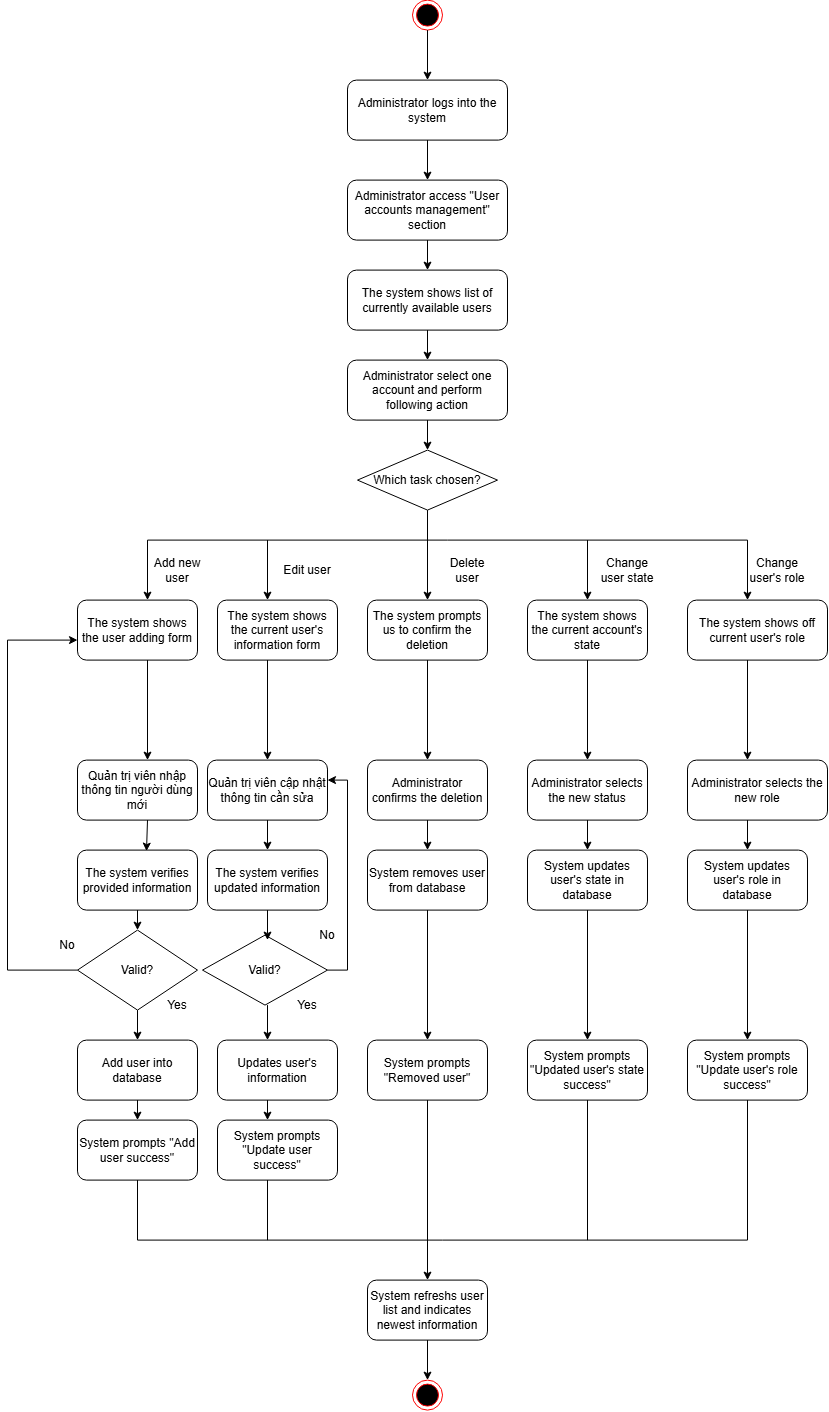
\includegraphics[width=0.6\linewidth]{Images/quanly.png}
	\vspace{10pt}
	\caption{Sơ đồ Hoạt động cho Quản lý Tài khoản Người dùng}
	\label{fig:activity_manage_users}
\end{figure}

\begin{enumerate}
	\item Admin đăng nhập và truy cập "Quản lý Người dùng".
	\item Hệ thống hiển thị danh sách người dùng (ID, Tên, Email, Vai trò, Trạng thái).
	\item Admin chọn người dùng đích và một thao tác (Thêm người dùng, Sửa hồ sơ, Xóa người dùng, Chuyển trạng thái, Thay đổi vai trò).
	\item Thực hiện quy trình đã chọn; hệ thống kiểm tra dữ liệu đầu vào và cập nhật DB, hiển thị thông báo thành công khi hoàn tất.
\end{enumerate}

\subsubsection{Thêm / Sửa / Xóa Bản ghi Danh mục}

\begin{figure}[H]
	\centering
	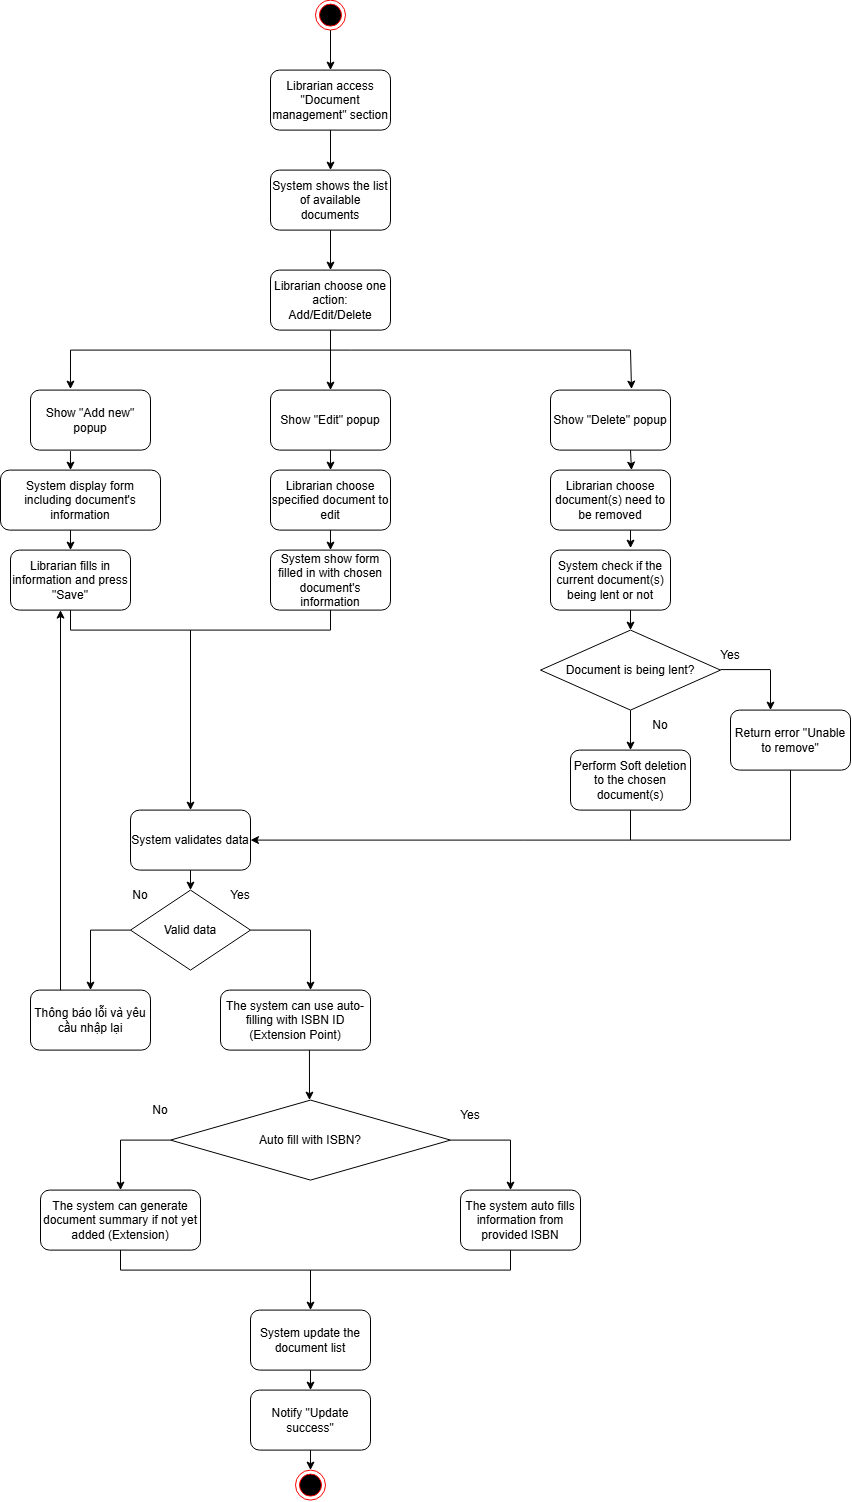
\includegraphics[width=0.6\linewidth]{Images/edit.png}
	\vspace{10pt}
	\caption{Sơ đồ Hoạt động cho Thêm / Sửa / Xóa Bản ghi Danh mục}
	\label{fig:activity_manage_documents}
\end{figure}

\begin{enumerate}
	\item Thủ thư mở "Quản lý Danh mục".
	\item Thủ thư chọn thao tác: Thêm, Sửa, hoặc Xóa.
	\item Nếu Xóa: Hệ thống kiểm tra các bản mượn đang hoạt động. Nếu tài liệu đang được mượn, chặn xóa ("Không thể xóa: Tài liệu đang được mượn"). Nguợc lại, thực hiện xóa mềm (Soft Delete).
	\item Nếu Thêm/Sửa: Biểu mẫu được hiển thị; có thể kích hoạt tùy chọn tự động biên mục qua ISBN (UC-CAT-03) hoặc tạo tóm tắt AI (UC-CAT-04).
	\item Hệ thống kiểm tra các trường, lưu cập nhật và báo thành công.
\end{enumerate}

\subsubsection{Nhập Dữ liệu Danh mục Hàng loạt}

\begin{figure}[H]
	\centering
	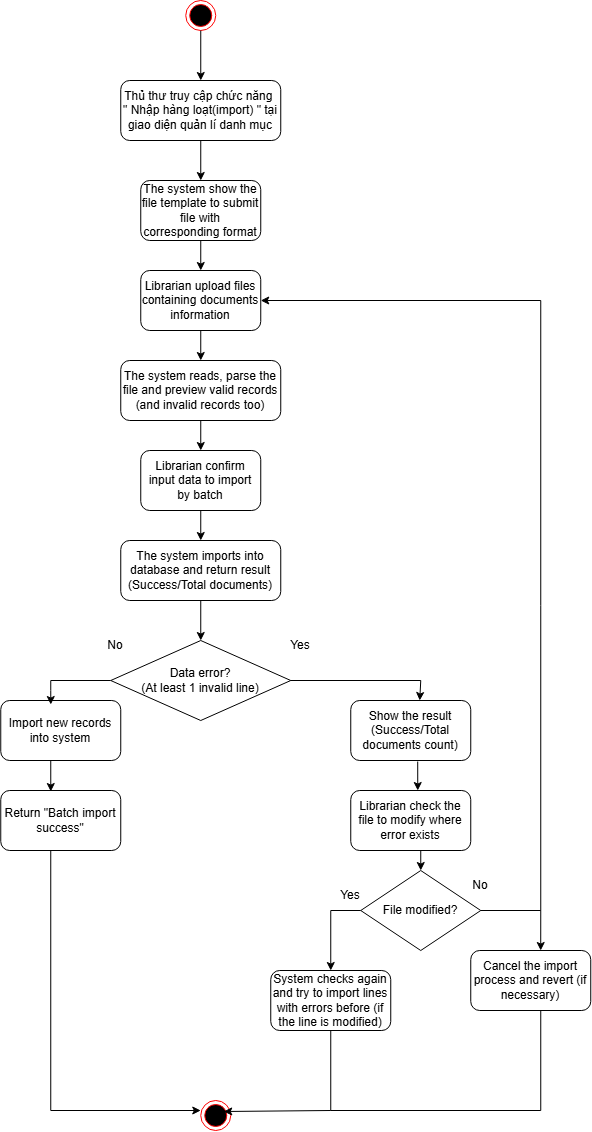
\includegraphics[width=0.6\linewidth]{Images/nhap.png}
	\vspace{10pt}
	\caption{Sơ đồ Hoạt động cho Nhập Dữ liệu Danh mục Hàng loạt}
	\label{fig:activity_import}
\end{figure}

\begin{enumerate}
	\item Thủ thư chọn "Nhập Hàng loạt".
	\item Tải lên tệp dữ liệu danh mục (CSV/Excel).
	\item Hệ thống đọc tệp và hiển thị bảng xem trước với số lượng bản ghi hợp lệ/không hợp lệ.
	\item Thủ thư xác nhận thực hiện nhập.
	\item Hệ thống ghi các dòng hợp lệ vào DB và báo cáo kết quả. Nếu có lỗi, thủ thư có thể sửa tệp và tải lại hoặc hủy thao tác.
\end{enumerate}

\subsubsection{Biên mục Tự động qua ISBN}

\begin{figure}[H]
	\centering
	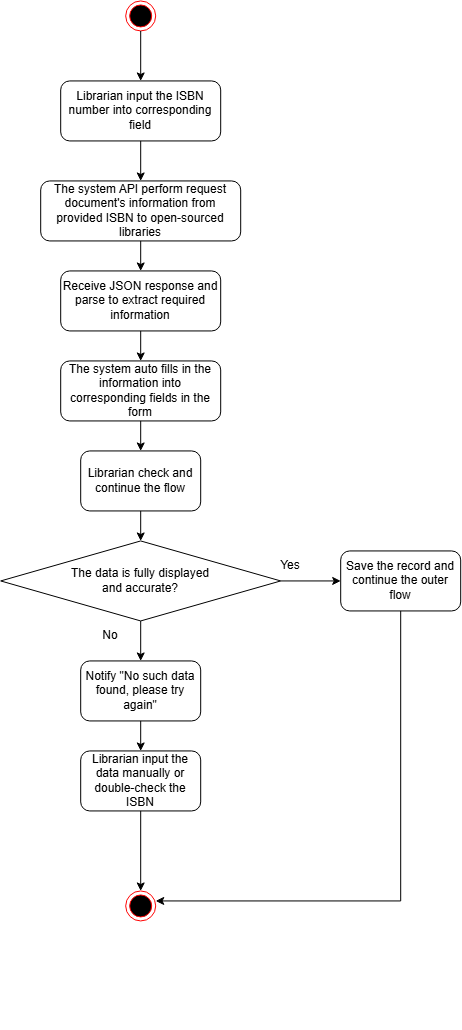
\includegraphics[width=0.6\linewidth]{Images/bienmuc.png}
	\vspace{10pt}
	\caption{Sơ đồ Hoạt động cho Biên mục Tự động qua ISBN}
	\label{fig:activity_isbn}
\end{figure}

\begin{enumerate}
	\item Thủ thư nhập mã ISBN.
	\item Hệ thống gửi yêu cầu API đến các nguồn bên ngoài (Google Books, Open Library).
	\item Phân tích phản hồi JSON và điền vào các trường biểu mẫu.
	\item Thủ thư xem lại và lưu bản ghi danh mục. Nếu không tìm thấy ISBN, thủ thư chuyển sang nhập thủ công.
\end{enumerate}

\subsubsection{Mượn Tài liệu Vật lý}

\begin{figure}[H]
	\centering
	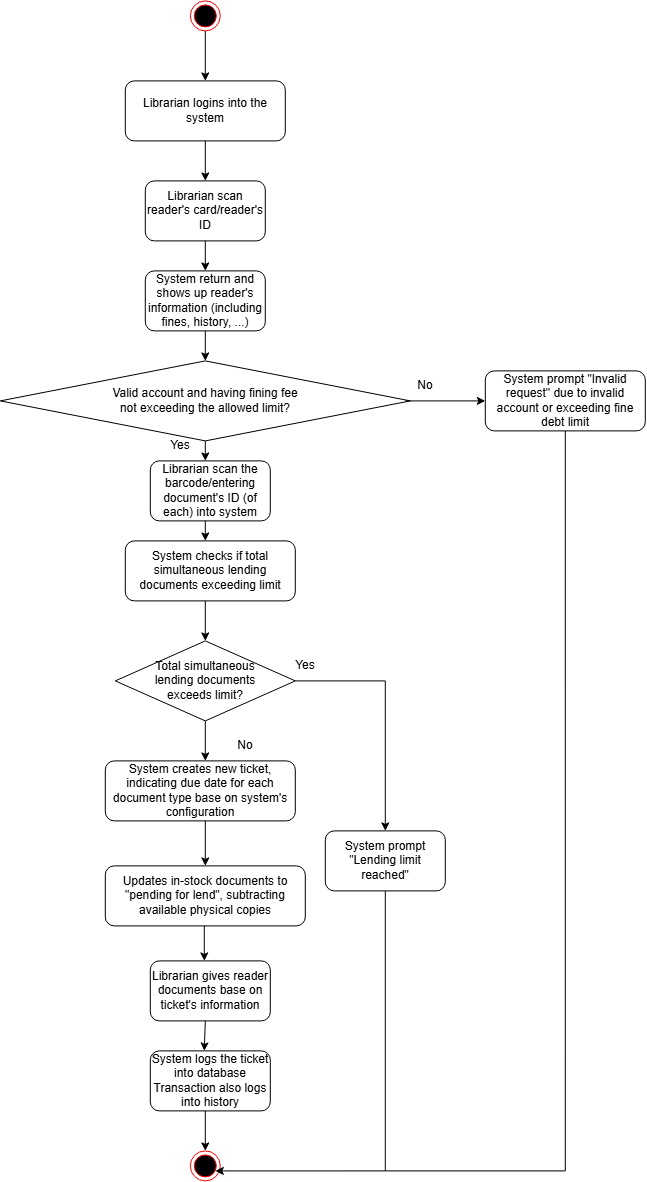
\includegraphics[width=0.6\linewidth]{Images/muon.png}
	\vspace{10pt}
	\caption{Sơ đồ Hoạt động cho Mượn Tài liệu Vật lý}
	\label{fig:activity_borrow}
\end{figure}

\begin{enumerate}
	\item Thủ thư đăng nhập và quét mã vạch thẻ Độc giả.
	\item Hệ thống kiểm tra trạng thái tài khoản và số tiền phạt chưa thanh toán.
	\item Nếu đủ điều kiện, thủ thư quét mã vạch các tài liệu mượn.
	\item Hệ thống kiểm tra hạn mức mượn theo vai trò và hạn chế từ hàng chờ đặt chỗ.
	\item Tạo bản ghi mượn, tính hạn trả, cập nhật trạng thái bản sao thành "Đã mượn" và giảm số lượng kho.
\end{enumerate}

\subsubsection{Trả Tài liệu}

\begin{figure}[H]
	\centering
	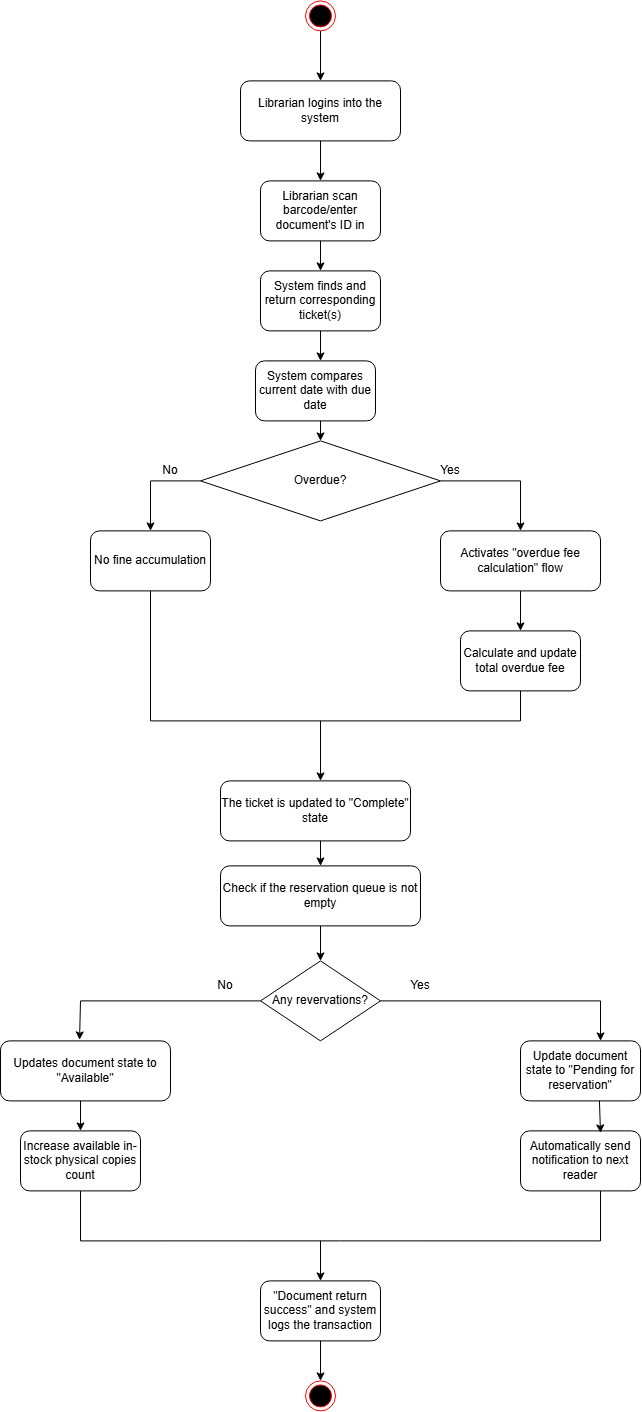
\includegraphics[width=0.6\linewidth]{Images/tra.png}
	\vspace{10pt}
	\caption{Sơ đồ Hoạt động cho Trả Tài liệu}
	\label{fig:activity_return}
\end{figure}

\begin{enumerate}
	\item Thủ thư quét mã vạch tài liệu trả.
	\item Hệ thống lấy bản ghi mượn và kiểm tra hạn trả.
	\item Nếu quá hạn, kích hoạt quy trình tính phạt (UC-CIR-03).
	\item Đặt trạng thái lượt mượn thành "Hoàn thành".
	\item Kiểm tra hàng chờ đặt chỗ: nếu có lượt đặt, đặt bản sao thành "Chờ lấy sách" và thông báo cho người dùng tiếp theo; nếu không có lượt đặt, đặt bản sao thành "Khả dụng".
\end{enumerate}

\subsubsection{Tính và Thu Phạt Quá hạn}

\begin{figure}[H]
	\centering
	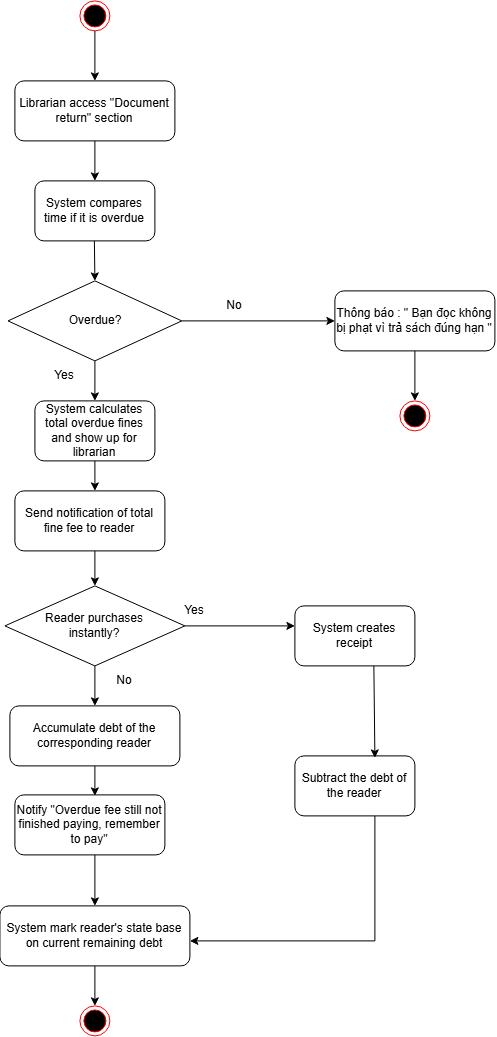
\includegraphics[width=0.5\linewidth]{Images/phiphat.png}
	\vspace{10pt}
	\caption{Sơ đồ Hoạt động cho Tính và Thu Phạt Quá hạn}
	\label{fig:activity_fine}
\end{figure}

\begin{enumerate}
	\item Hệ thống tính số ngày quá hạn (Ngày trả - Hạn trả), loại trừ các ngày lễ của thư viện.
	\item Nhân số ngày quá hạn với mức phí phạt hằng ngày.
	\item Hiển thị khoản phạt tính toán. Nếu độc giả thanh toán ngay, xuất hóa đơn và đặt số dư phạt về 0; ngược lại ghi khoản phạt vào sổ nợ tài khoản độc giả.
\end{enumerate}

\subsubsection{Gia hạn Mượn Trực tuyến}

\begin{figure}[H]
	\centering
	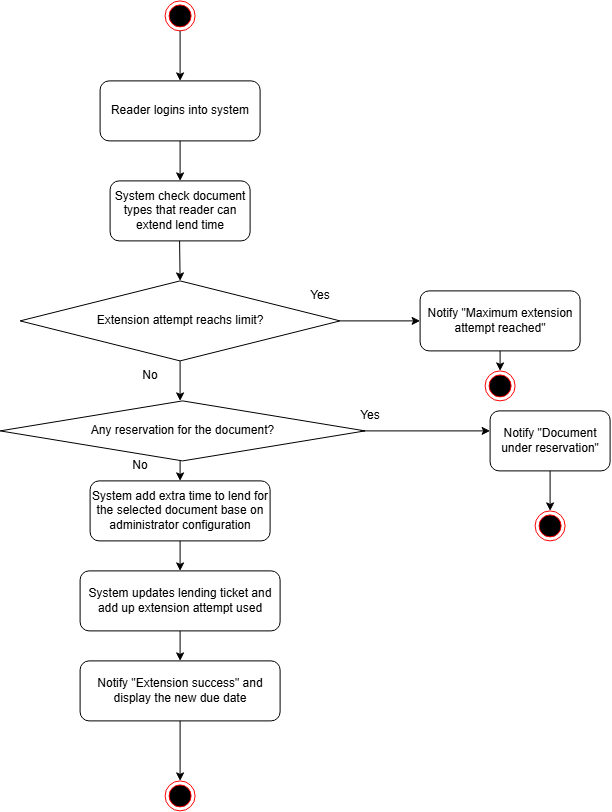
\includegraphics[width=0.6\linewidth]{Images/giahan.png}
	\vspace{10pt}
	\caption{Sơ đồ Hoạt động cho Gia hạn Mượn Trực tuyến}
	\label{fig:activity_extend}
\end{figure}

\begin{enumerate}
	\item Độc giả mở danh sách mượn hiện tại và nhấn "Gia hạn".
	\item Hệ thống kiểm tra: chưa vượt quá số lần gia hạn tối đa và không có yêu cầu đặt chỗ nào khác.
	\item Nếu đủ điều kiện, kéo dài hạn trả, tăng số lần gia hạn và hiển thị hạn trả mới.
\end{enumerate}

\subsubsection{Đặt Giữ chỗ Tài liệu}

\begin{figure}[H]
	\centering
	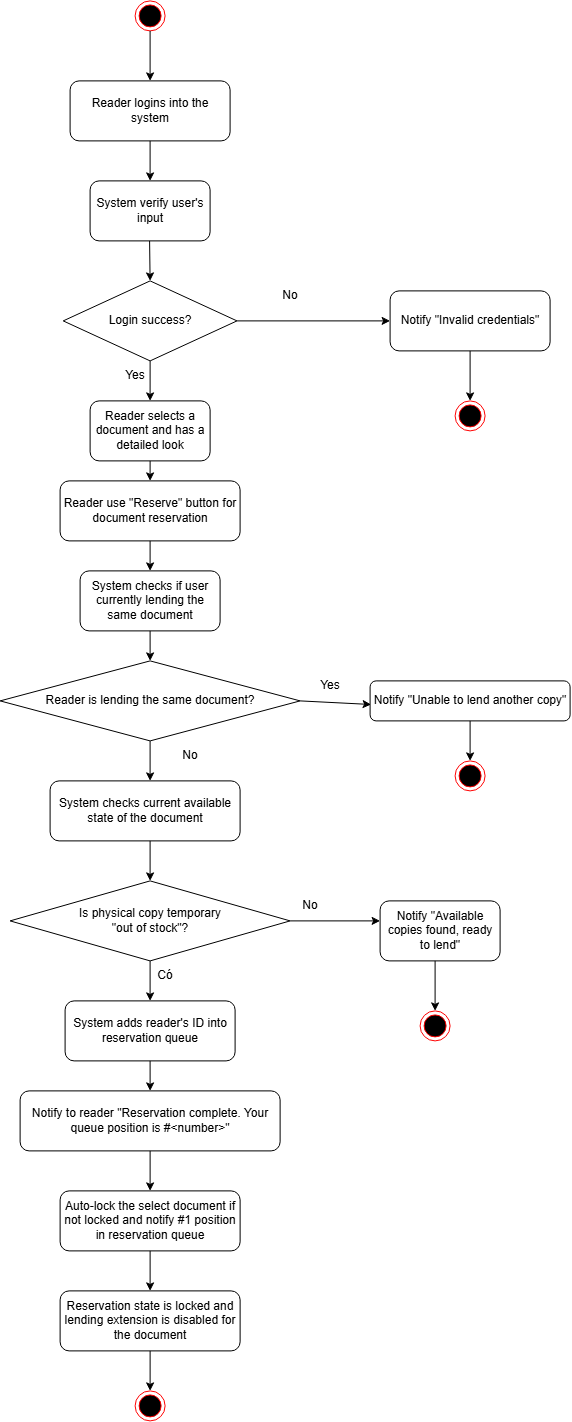
\includegraphics[width=0.5\linewidth]{Images/dat.png}
	\vspace{10pt}
	\caption{Sơ đồ Hoạt động cho Đặt Giữ chỗ Tài liệu}
	\label{fig:activity_reserve}
\end{figure}

\begin{enumerate}
	\item Độc giả mở trang chi tiết tài liệu và nhấn "Đặt chỗ".
	\item Hệ thống kiểm tra độc giả hiện không mượn tài liệu này và tất cả các bản sao đều đã được mượn hết.
	\item Hệ thống thêm độc giả vào hàng chờ đặt chỗ và hiển thị vị trí trong hàng chờ.
\end{enumerate}

\subsubsection{Tìm kiếm Danh mục Tài liệu}

\begin{figure}[H]
	\centering
	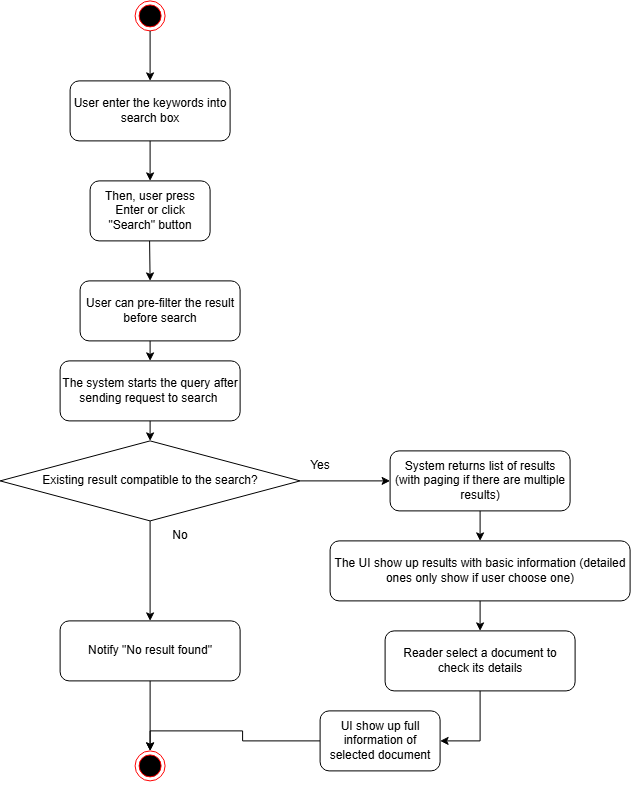
\includegraphics[width=0.6\linewidth]{Images/tracuu.png}
	\vspace{10pt}
	\caption{Sơ đồ Hoạt động cho Tìm kiếm Danh mục Tài liệu}
	\label{fig:activity_search}
\end{figure}

\begin{enumerate}
	\item Độc giả nhập từ khóa tìm kiếm và chọn tiêu chí tra cứu.
	\item Hệ thống truy vấn các chỉ mục cơ sở dữ liệu danh mục và trả về kết quả phân trang.
	\item Hiển thị thẻ sách. Độc giả nhấn vào thẻ sách để xem trang chi tiết.
\end{enumerate}

\subsection{Sơ đồ Tuần tự (Sequence Diagrams)}

\subsubsection{Đăng ký Tài khoản}
\begin{figure}[H]
	\centering
	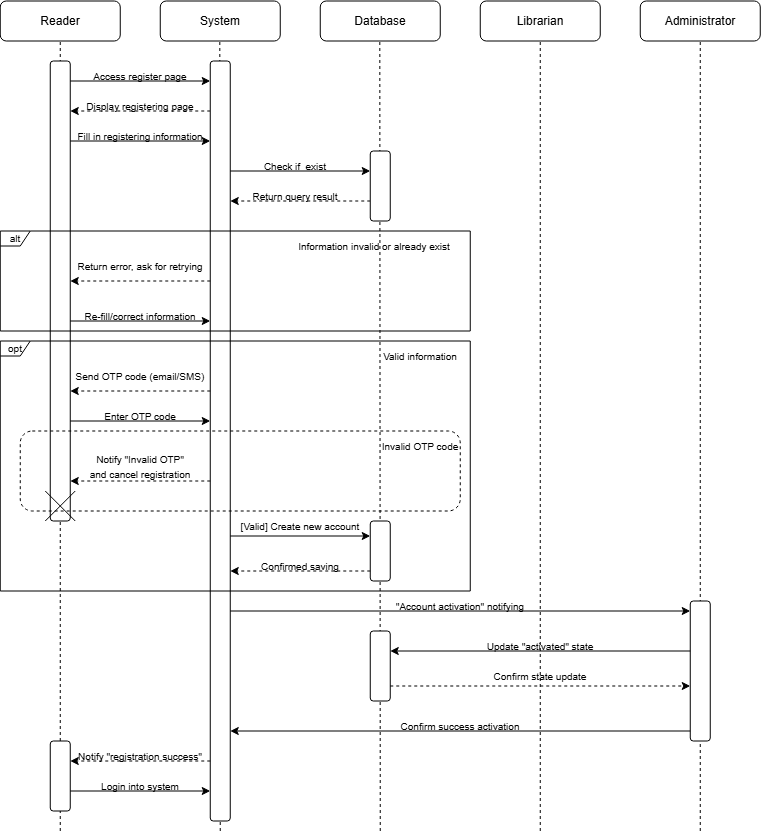
\includegraphics[width=0.6\linewidth]{Images/Seq_Dang ky.png}
	\vspace{10pt}
	\caption{Sơ đồ Tuần tự cho Đăng ký Tài khoản}
	\label{fig:sequence_register}
\end{figure}
\begin{enumerate}
	\item Độc giả truy cập giao diện đăng ký.
	\item Gửi thông tin; hệ thống kiểm tra dữ liệu và trùng lặp.
	\item Hệ thống gửi mã OTP qua email/SMS.
	\item Độc giả nhập OTP. Nếu OTP hợp lệ, tài khoản được tạo và kích hoạt; ngược lại quá trình đăng ký bị hủy.
\end{enumerate}

\subsubsection{Đăng nhập Hệ thống}
\begin{figure}[H]
	\centering
	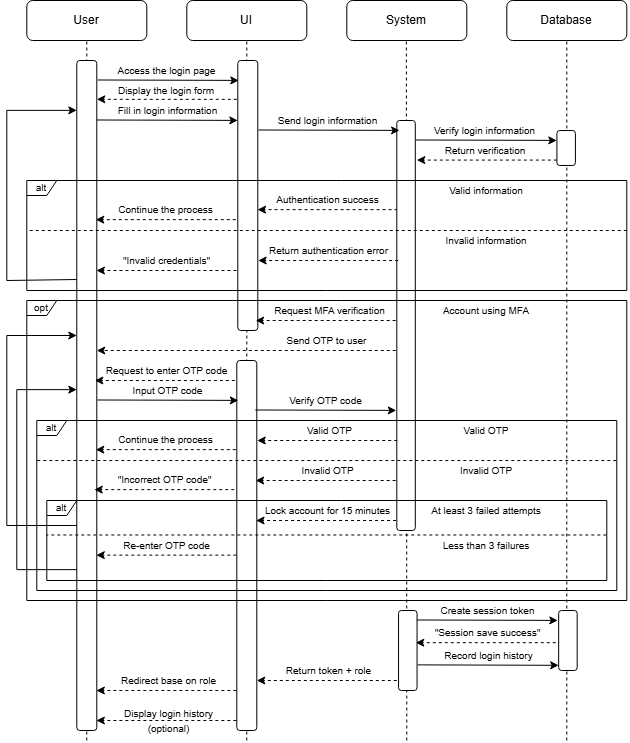
\includegraphics[width=0.6\linewidth]{Images/Seq_Dang nhap.png}
	\vspace{10pt}
	\caption{Sơ đồ Tuần tự cho Đăng nhập Hệ thống}
	\label{fig:sequence_login}
\end{figure}
\begin{enumerate}
	\item Người dùng gửi thông tin đăng nhập.
	\item Hệ thống đối chiếu thông tin với DB.
	\item Nếu bật MFA, yêu cầu mã OTP; khi xác thực OTP thành công, cấp session JWT token và chuyển hướng người dùng đến bảng điều khiển theo vai trò.
\end{enumerate}

\subsubsection{Đặt lại Mật khẩu Tài khoản}
\begin{figure}[H]
	\centering
	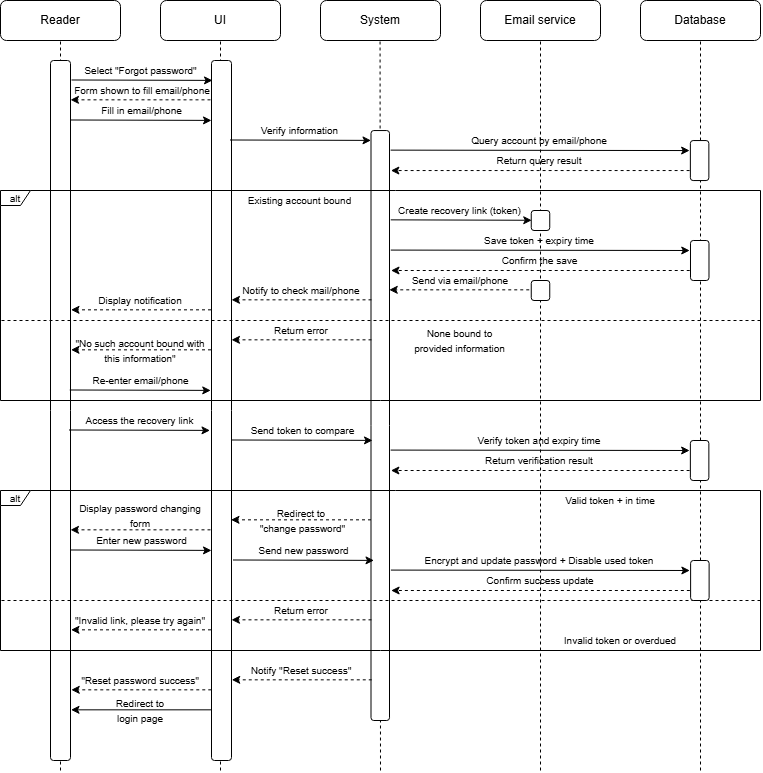
\includegraphics[width=0.6\linewidth]{Images/Seq_Reset mat khau.png}
	\vspace{10pt}
	\caption{Sơ đồ Tuần tự cho Đặt lại Mật khẩu Tài khoản}
	\label{fig:sequence_reset_password}
\end{figure}
\begin{enumerate}
	\item Người dùng yêu cầu đặt lại mật khẩu bằng cách nhập email đã đăng ký.
	\item Hệ thống xác minh email, tạo reset token và gửi liên kết đặt lại qua email.
	\item Người dùng mở liên kết; hệ thống xác thực token. Người dùng gửi mật khẩu mới; hệ thống cập nhật băm mật khẩu.
\end{enumerate}

\subsubsection{Tìm kiếm Tài liệu}
\begin{figure}[H]
	\centering
	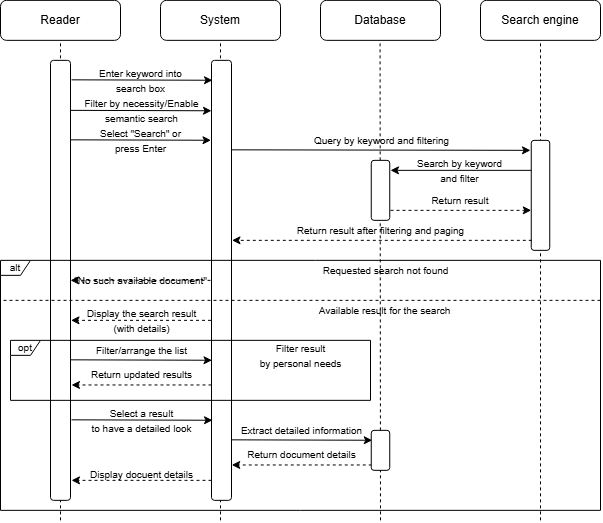
\includegraphics[width=0.6\linewidth]{Images/Seq_Tim kiem.png}
	\vspace{10pt}
	\caption{Sơ đồ Tuần tự cho Tìm kiếm Tài liệu}
	\label{fig:sequence_search}
\end{figure}
\begin{enumerate}
	\item Độc giả nhập câu truy vấn tìm kiếm.
	\item Công cụ tìm kiếm truy vấn cơ sở dữ liệu danh mục và trả về kết quả đã lọc và phân trang.
	\item Hiển thị các thẻ tài liệu; nhấn vào tài liệu để lấy bản ghi chi tiết.
\end{enumerate}

\subsubsection{Thêm / Sửa / Xóa Tài liệu}
\subsubsubsection{Thêm Tài liệu}
\begin{figure}[H]
	\centering
	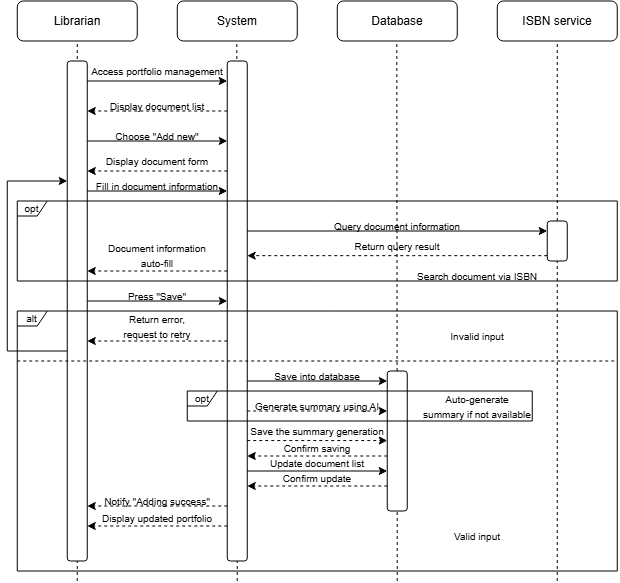
\includegraphics[width=0.6\linewidth]{Images/Seq_Them tai lieu.png}
	\vspace{10pt}
	\caption{Sơ đồ Tuần tự cho Thêm Tài liệu}
	\label{fig:sequence_add_document}
\end{figure}
Thủ thư nhập dữ liệu tả thủ công hoặc lấy qua ISBN API (UC-CAT-03), có thể tạo tóm tắt AI (UC-CAT-04), và lưu bản ghi.

\subsubsubsection{Sửa Tài liệu}
\begin{figure}[H]
	\centering
	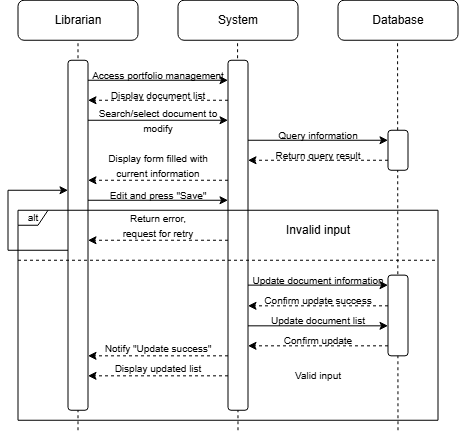
\includegraphics[width=0.6\linewidth]{Images/Seq_Sua tai lieu.png}
	\vspace{10pt}
	\caption{Sơ đồ Tuần tự cho Sửa Tài liệu}
	\label{fig:sequence_edit_document}
\end{figure}
Thủ thư chỉnh sửa các trường tài liệu đã điền sẵn, hệ thống kiểm tra dữ liệu đầu vào và cập nhật bản ghi DB.

\subsubsubsection{Xóa Tài liệu}
\begin{figure}[H]
	\centering
	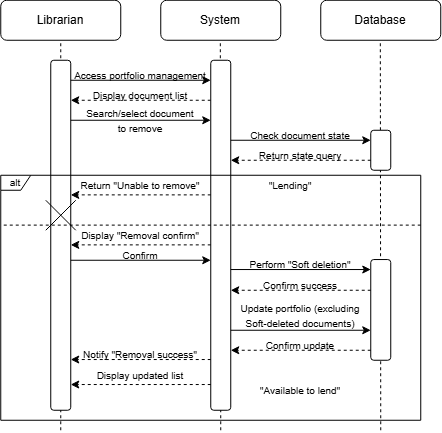
\includegraphics[width=0.6\linewidth]{Images/Seq_Xoa tai lieu.png}
	\vspace{10pt}
	\caption{Sơ đồ Tuần tự cho Xóa Tài liệu}
	\label{fig:sequence_delete_document}
\end{figure}
Hệ thống xác minh tài liệu hiện không được mượn, thủ thư xác nhận xóa và hệ thống thực hiện xóa mềm.

\subsubsection{Nhập Tài liệu Hàng loạt}
\begin{figure}[H]
	\centering
	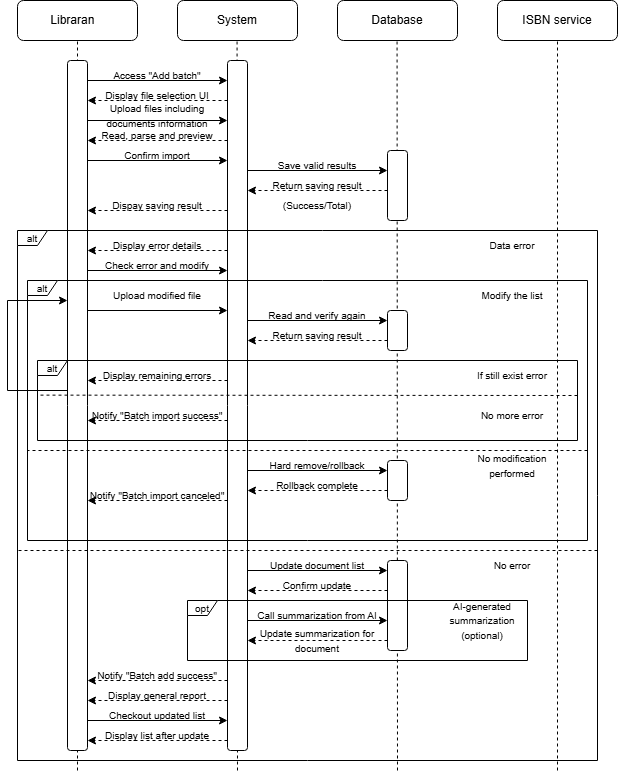
\includegraphics[width=0.6\linewidth]{Images/Seq_Them hang loat.png}
	\vspace{10pt}
	\caption{Sơ đồ Tuần tự cho Nhập Tài liệu Hàng loạt}
	\label{fig:sequence_import_documents}
\end{figure}
Thủ thư tải tệp lên; hệ thống kiểm tra các dòng, nhập các dòng hợp lệ và báo cáo tổng hợp lỗi.

\subsubsection{Đặt Giữ chỗ Tài liệu}
\begin{figure}[H]
	\centering
	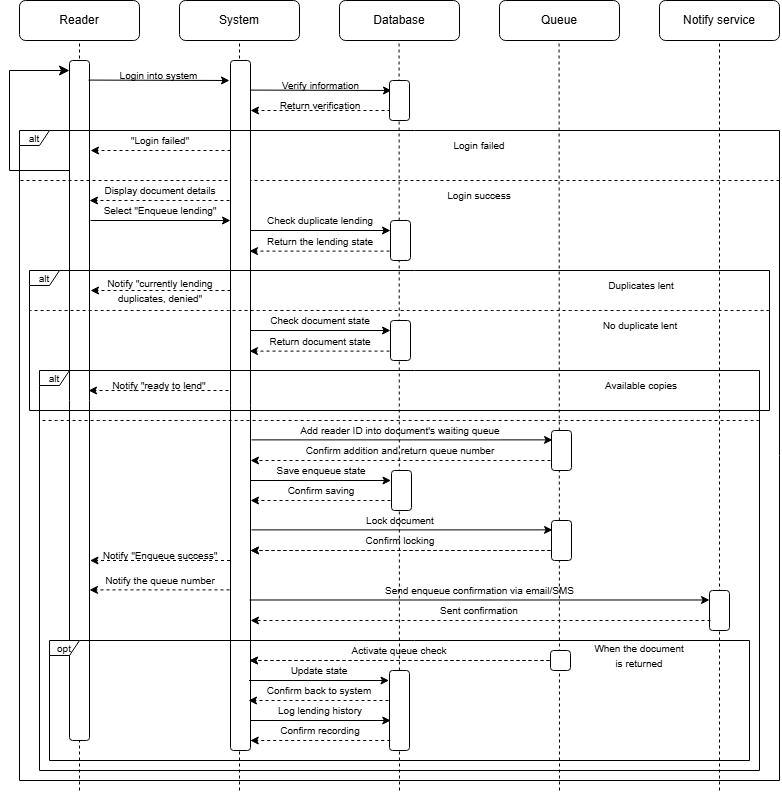
\includegraphics[width=0.6\linewidth]{Images/Seq_Dat muon sach.png}
	\vspace{10pt}
	\caption{Sơ đồ Tuần tự cho Đặt Giữ chỗ Tài liệu}
	\label{fig:sequence_reserve_document}
\end{figure}
Hệ thống kiểm tra trùng lặp lượt mượn và tình trạng bản sao khả dụng; nếu không còn bản sao khả dụng nào, thêm người dùng vào hàng chờ và gửi email xác nhận.

\subsubsection{Cập nhật Tính Phạt}
\begin{figure}[H]
	\centering
	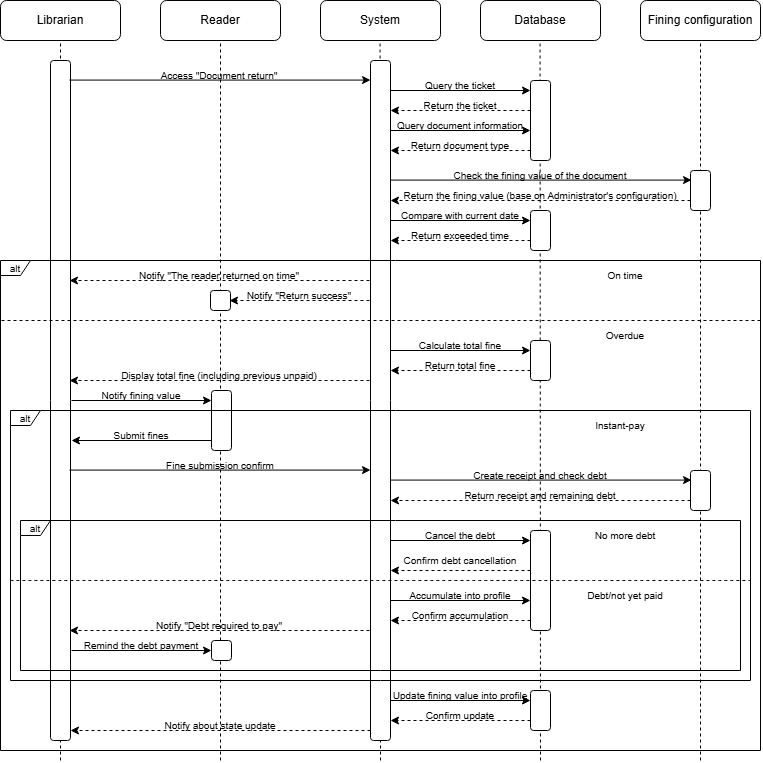
\includegraphics[width=0.6\linewidth]{Images/Seq_Tien phat.png}
	\vspace{10pt}
	\caption{Sơ đồ Tuần tự cho Cập nhật Tính Phạt}
	\label{fig:sequence_fine}
\end{figure}
Hệ thống kiểm tra ngưỡng phạt của độc giả, quét tài liệu, tạo phiếu mượn và giảm số lượng kho.

\subsubsection{Xử lý Mượn Tài liệu}
\begin{figure}[H]
	\centering
	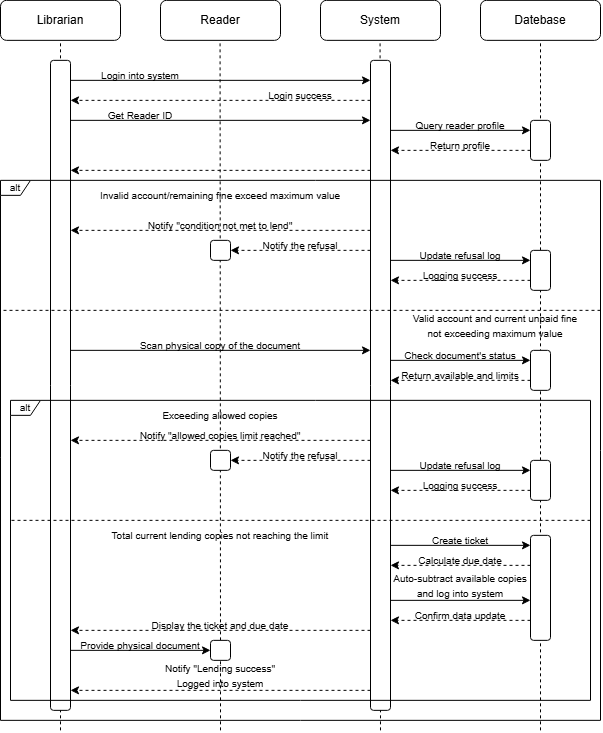
\includegraphics[width=0.6\linewidth]{Images/Seq_Muon sach.png}
	\vspace{10pt}
	\caption{Sơ đồ Tuần tự cho Xử lý Mượn Tài liệu}
	\label{fig:sequence_borrow}
\end{figure}
Thủ thư xác minh điều kiện độc giả, kiểm tra trạng thái giữ chỗ tài liệu, kiểm tra hạn mức mượn và tạo phiếu mượn.

\subsubsection{Gia hạn Mượn Tài liệu}
\begin{figure}[H]
	\centering
	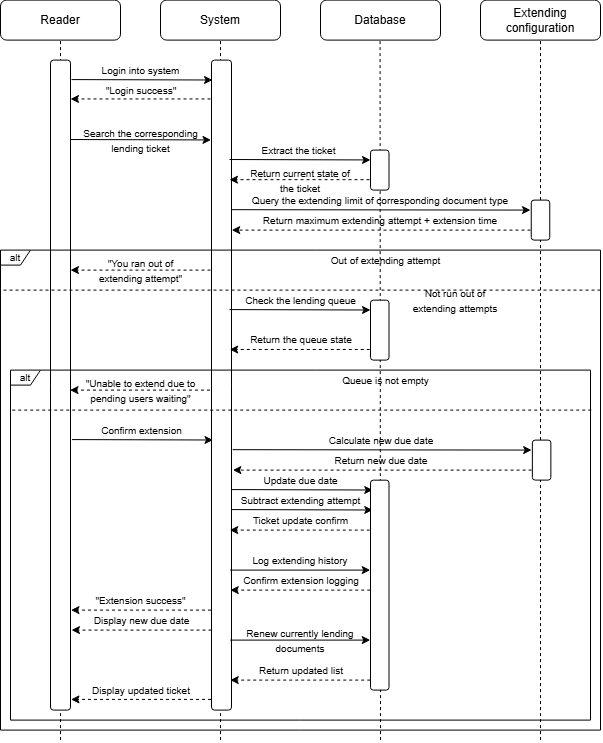
\includegraphics[width=0.6\linewidth]{Images/Seq_Gia han.png}
	\vspace{10pt}
	\caption{Sơ đồ Tuần tự cho Gia hạn Mượn Tài liệu}
	\label{fig:sequence_extend_borrow}
\end{figure}
Hệ thống kiểm tra số lần gia hạn cho phép và trạng thái hàng chờ đặt chỗ; kéo dài hạn trả khi được chấp thuận.

\subsubsection{Trả Tài liệu}
\begin{figure}[H]
	\centering
	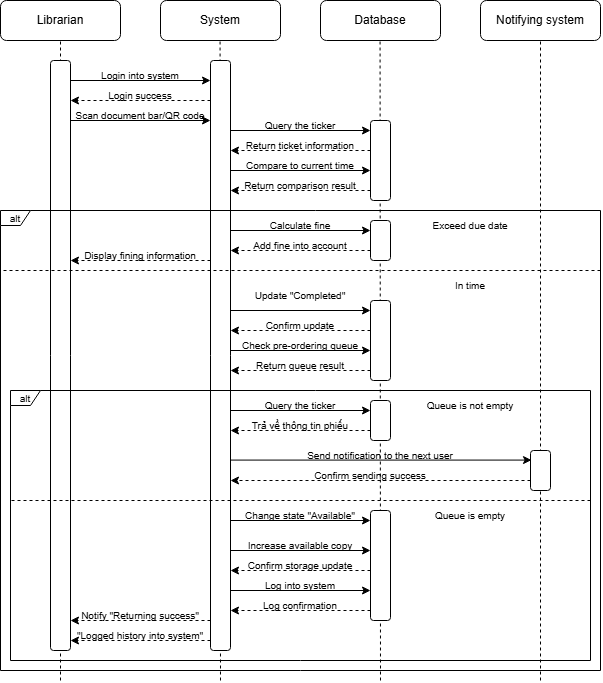
\includegraphics[width=0.6\linewidth]{Images/Seq_Tra sach.png}
	\vspace{10pt}
	\caption{Sơ đồ Tuần tự cho Trả Tài liệu}
	\label{fig:sequence_return}
\end{figure}
Thủ thư quét tài liệu, hệ thống tính phạt quá hạn nếu có, kiểm tra hàng chờ đặt chỗ, cập nhật trạng thái bản sao và đóng phiếu mượn.
\newpage
\begingroup
\fontencoding{T5}\selectfont
\section{Hiện thực Hệ thống}

Chương này mô tả chi tiết việc hiện thực Hệ thống Quản lý Thư viện Trực tuyến BkLib. Đầu tiên, chương giới thiệu về công nghệ và các thành phần kiến trúc vận hành nền tảng, tiếp theo là chi tiết từng mô-đun bao gồm cả giao diện người dùng và hiện thực kỹ thuật cốt lõi (dịch vụ backend, logic nghiệp vụ và các đoạn mã nguồn tiêu biểu).

% =========================================================================
% SECTION 5.1: TECHNOLOGY STACK
% =========================================================================
\subsection{Tập công nghệ (Technology Stack)}

\subsubsection{Front-end: React.js và Vite}
React.js đảm nhận tầng giao diện của thư viện trực tuyến, xây dựng các giao diện tương tác cho việc tìm kiếm sách, duyệt danh mục và trò chuyện với trợ lý AI. Vite được sử dụng làm công cụ đóng gói và máy chủ phát triển giúp khởi động nhanh, hỗ trợ HMR (Hot Module Replacement) và tối ưu hóa việc biên dịch sản phẩm. Phía máy khách, các thành phần xử lý việc hiển thị kết quả tìm kiếm (kết hợp tô sáng từ khóa và khớp ngữ nghĩa), quản lý trạng thái người dùng (cache, cập nhật lạc quan) và tích hợp SDK chatbot/trợ lý AI (phản hồi dạng streaming, trạng thái hội thoại).
\begin{figure}[htbp]
    \centering
    
\includegraphics[width=0.4\textwidth]{Images/react_vite.png}
\end{figure}

\subsubsection{Back-end: Node.js và Express}
Node.js + Express cung cấp các REST API cốt lõi cho việc quản lý danh mục sách, tài khoản người dùng và quản trị phiên làm việc. Máy chủ điều phối việc định tuyến yêu cầu, xác thực, phân quyền RBAC, các giao dịch PostgreSQL thông qua Prisma và ủy quyền các tác vụ AI (tạo vector nhúng, tóm tắt, truy vấn RAG) cho dịch vụ AI chuyên biệt. Máy chủ cung cấp các điểm cuối API tiêu chuẩn cho tìm kiếm, gợi ý và tích hợp webhook (ví dụ: làm giàu dữ liệu tả từ Open Library).
\begin{figure}[htbp]
    \centering
    
\includegraphics[width=0.4\textwidth]{Images/node_express.jpg}
\end{figure}

\subsubsection{Dịch vụ AI Microservice Chuyên biệt: Python và FastAPI}
Dịch vụ microservice độc lập được triển khai bằng Python + FastAPI tận dụng các thư viện Xử lý Ngôn ngữ Tự nhiên (NLP) và Mã nguồn Mở Machine Learning (transformers, sentence-transformers, SDK client của các nhà cung cấp LLM). Nhiệm vụ chính bao gồm tạo vector nhúng, tóm tắt tài liệu, trả lời câu hỏi dựa trên RAG và các đường ống xử lý prompt (chia đoạn, xếp hạng lại). FastAPI là lựa chọn lý tưởng cho các điểm cuối API bất đồng bộ độ trễ thấp và có thể mở rộng linh hoạt theo tải công việc.
\begin{figure}[htbp]
    \centering
    
\includegraphics[width=0.4\textwidth]{Images/fastapi.png}
\end{figure}

\subsubsection{ORM: Prisma}
Prisma (TypeScript) được sử dụng để định nghĩa lược đồ cơ sở dữ liệu, tạo các truy vấn an toàn kiểu dữ liệu và quản lý các migration của PostgreSQL. Prisma duy trì tính an toàn kiểu end-to-end giữa ứng dụng Node và tầng cơ sở dữ liệu, đơn giản hóa các truy vấn liên quan đến lượt mượn, nhật ký giao dịch và dữ liệu tả danh mục đồng thời hỗ trợ giao dịch ACID cho tính nhất quán dữ liệu.
\begin{figure}[htbp]
    \centering
    
\includegraphics[width=0.4\textwidth]{Images/prisma.png}
\end{figure}

\subsubsection{Cơ sở Dữ liệu Quan hệ: PostgreSQL}
PostgreSQL đóng vai trò là kho lưu trữ quan hệ chính cho các bản ghi sách, hồ sơ người dùng, giao dịch mượn trả và dữ liệu tả hệ thống. Ưu điểm chính bao gồm sự tuân thủ nghiêm ngặt chuẩn ACID cho quy trình mượn trả, hỗ trợ JSONB nâng cao cho dữ liệu tả linh hoạt, chỉ mục từ khóa toàn văn (full-text search) và khả năng mở rộng ngang qua nhân bản và phân mảnh.
\begin{figure}[htbp]
    \centering
    
\includegraphics[width=0.4\textwidth]{Images/postgresql.jpg}
\end{figure}

\subsubsection{Kho Lưu trữ Vector và Embeddings: pgvector}
Các vector nhúng văn bản cho nội dung sách (toàn văn, tóm tắt) được lưu trữ trong `pgvector` (mở rộng vector cho PostgreSQL) hoặc cơ sở dữ liệu vector chuyên dụng. Kho vector thực hiện các phép tìm kiếm láng giềng gần nhất (độ tương đồng cosine) để phục vụ tìm kiếm ngữ nghĩa, truy xuất ngữ cảnh cho đường ống RAG và tính năng gợi ý "sách tương tự", ánh xạ kết quả vector trực tiếp đến ID tài liệu gốc.
\begin{figure}[htbp]
    \centering
    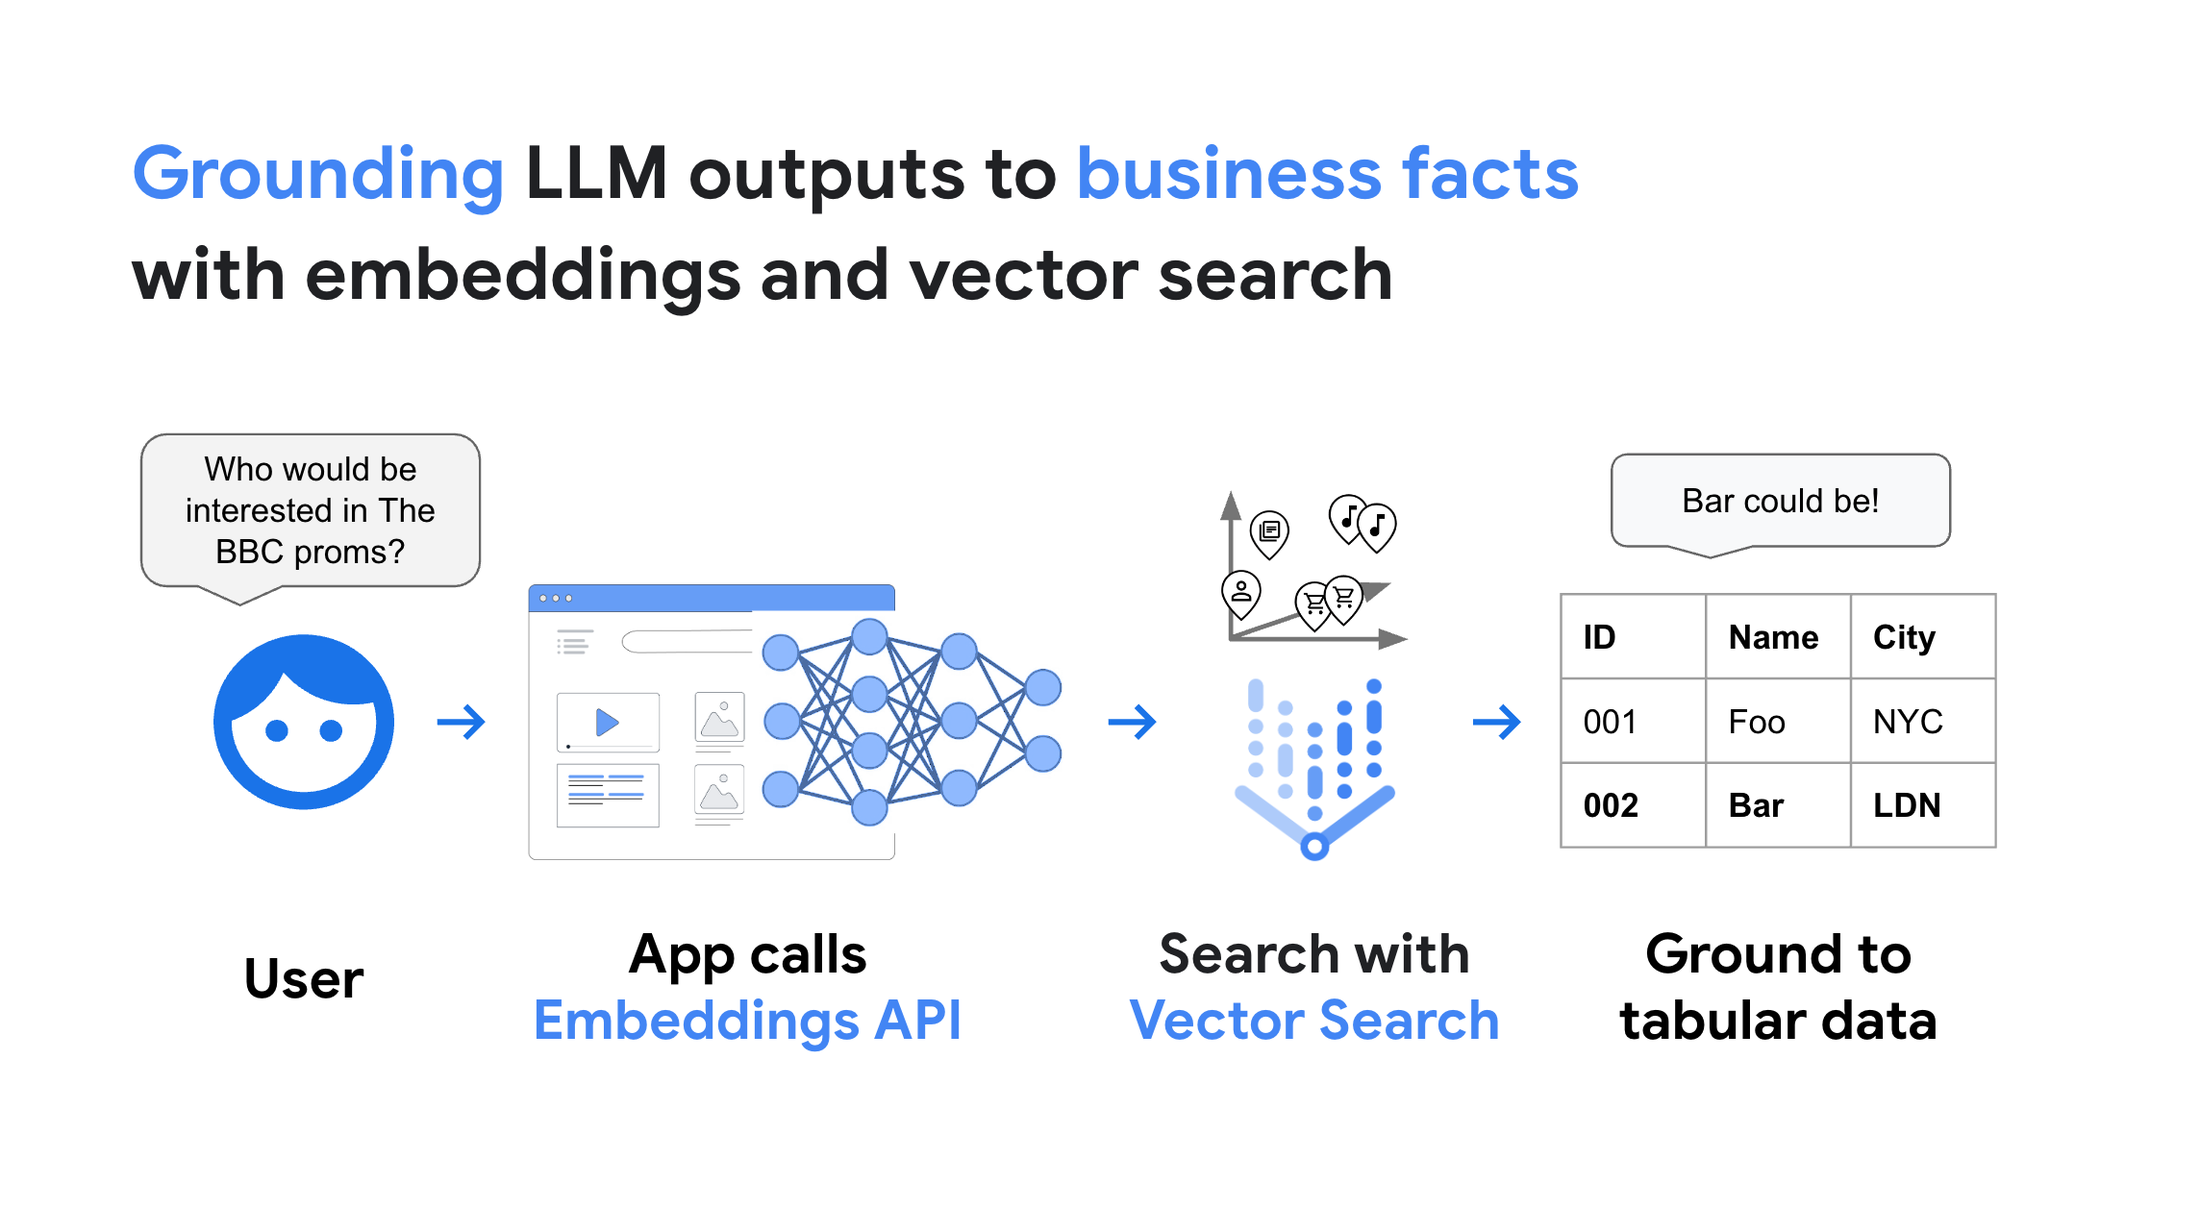
\includegraphics[width=0.5\textwidth]{Images/EmbeddingsAPI.png}
\end{figure}

\subsubsection{Chiến lược Tìm kiếm Kết hợp (Hybrid Search)}
Chiến lược tìm kiếm kết hợp phối hợp giữa: 1) tìm kiếm từ khóa toàn văn trên PostgreSQL để khớp dữ liệu tả chính xác; và 2) tìm kiếm tương đồng vector qua pgvector để truy xuất ngữ nghĩa và khớp ngữ cảnh. Kết quả được gộp và xếp hạng lại (dựa trên điểm độ liên quan, độ phổ biến và ngữ cảnh người dùng) trước khi trả về giao diện máy khách.

\subsubsection{An ninh và Xác thực: JWT, RBAC và OTP}
Hệ thống sử dụng JSON Web Token (JWT) cho quản lý phiên làm việc và refresh token cho sự duy trì an toàn. Kiểm soát Truy cập Dựa trên Vai trò (RBAC) áp dụng các quyền chi tiết (Admin, Thủ thư, Độc giả) được xác thực tại gateway API và các điểm cuối endpoints. Mật khẩu Một lần (OTP qua email/SMS) bảo vệ xác thực đa yếu tố cho các thao tác nhạy cảm. Các biện pháp bổ sung bao gồm mã hóa HTTPS/TLS, giới hạn tần suất gửi yêu cầu (rate limiting) và ghi nhật ký kiểm toán toàn diện.

\subsubsection{Tích hợp Bên ngoài: Open Library, Google Books và Nodemailer}
API Open Library và Google Books tự động hóa việc lấy dữ liệu tả, ảnh bìa và dữ liệu xuất bản qua mã ISBN. Một đường ống ETL tự động định kỳ đồng bộ dữ liệu danh mục. `Nodemailer` xử lý các thông báo giao dịch (nhắc hạn trả sách, đặt lại mật khẩu, cảnh báo hệ thống) với các mẫu HTML động và ghi nhật ký phân phối.
\begin{figure}[htbp]
    \centering
    
\includegraphics[width=0.3\textwidth]{Images/Google-play-book-icon.png}
\end{figure}

% =========================================================================
% SECTION 5.2: AUTHENTICATION MODULE
% =========================================================================
\subsection{Mô-đun Xác thực}

Mô-đun Xác thực đóng vai trò là cổng chính để truy cập hệ thống cho tất cả các vai trò người dùng trong hệ thống BkLib. Mô-đun thực thi xác minh danh tính an toàn, điều hướng truy cập dựa trên vai trò, đăng ký thành viên tự phục vụ, khôi phục mật khẩu đa bước và middleware phân quyền bằng JSON Web Token (JWT).

\subsubsection{Hiện thực Giao diện Người dùng}

\paragraph{Trang Đăng nhập}
Cổng truy cập chính cung cấp xác thực hợp nhất với các thẻ chuyển đổi vai trò.

\begin{figure}[H]
    \centering
    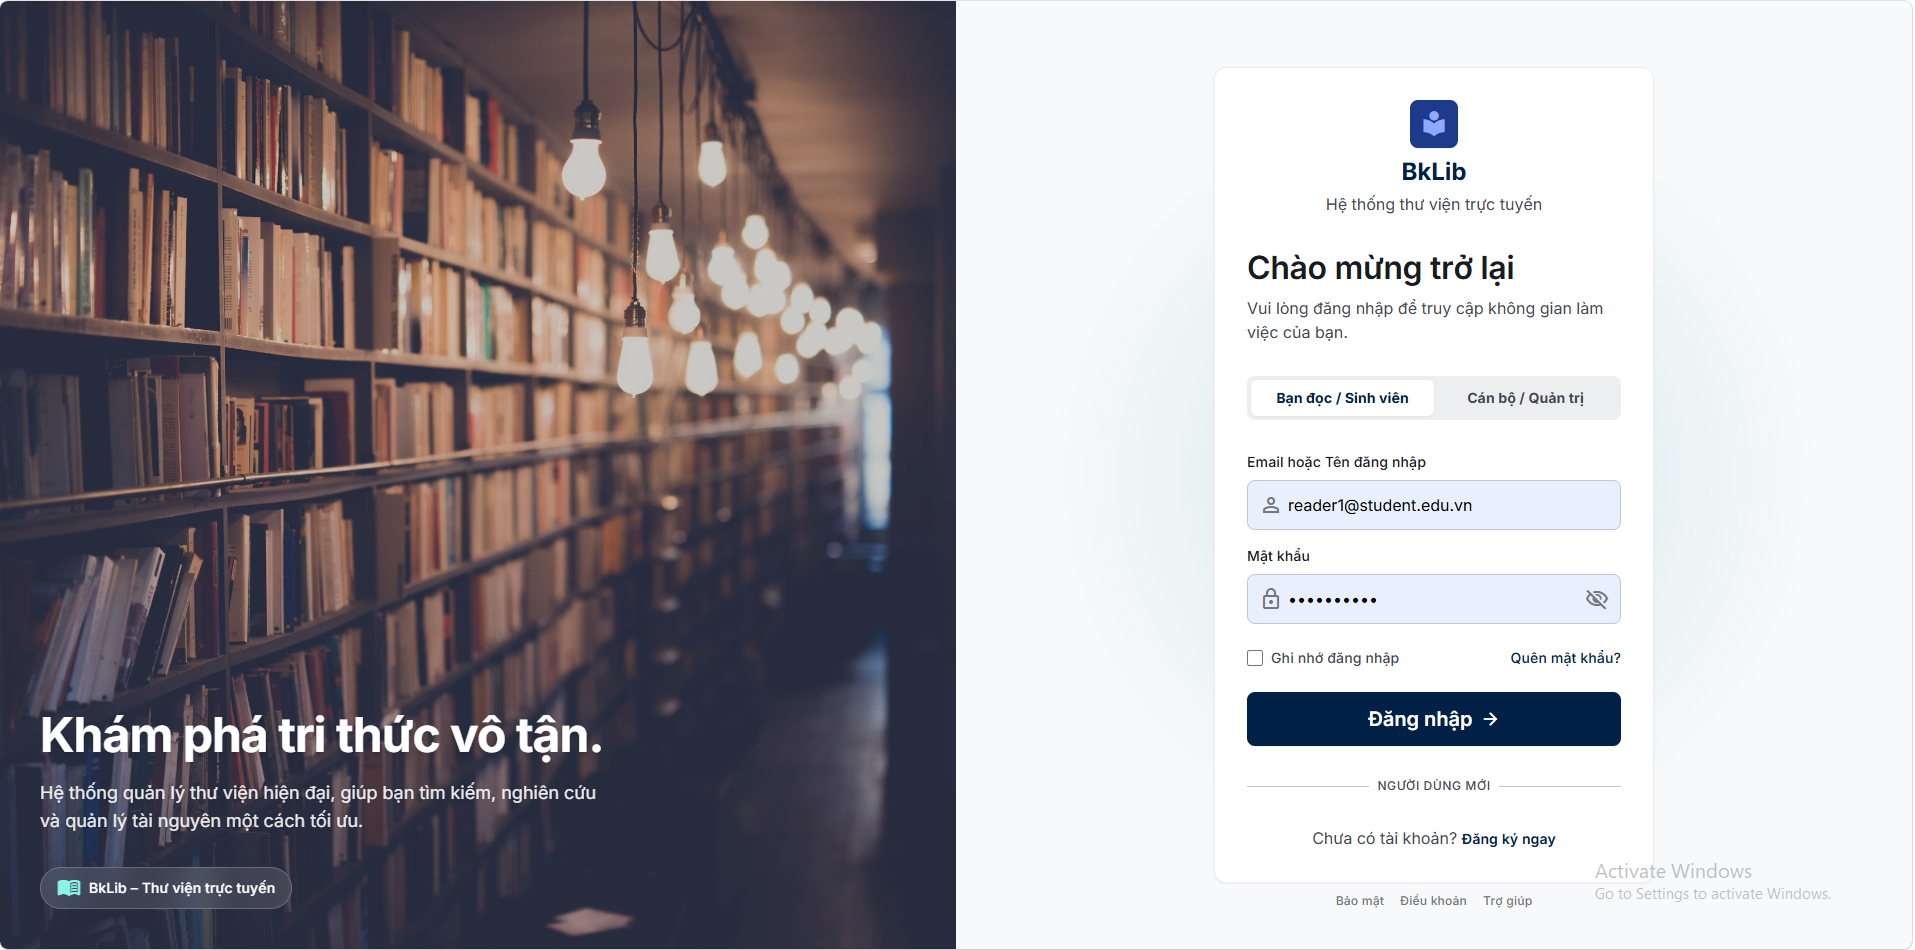
\includegraphics[width=0.95\linewidth]{Images/Auth_DangNhap.png}
    \vspace{10pt}
    \caption{Giao diện Đăng nhập BkLib}
    \label{fig:auth_login}
\end{figure}

\textbf{Bố cục \& Chức năng:} Thiết kế chia màn hình với hình ảnh thương hiệu ở bên trái và thẻ xác thực sạch sẽ ở bên phải. Bao gồm các tab lựa chọn vai trò ("Bạn đọc / Sinh viên" và "Cán bộ / Quản trị"), các trường nhập thông tin (email hoặc tên đăng nhập, mật khẩu có tùy chọn ẩn/hiện), hộp kiểm "Ghi nhớ đăng nhập", và các nút kích hoạt trực tiếp cho khôi phục mật khẩu ("Quên mật khẩu?") và đăng ký tài khoản. Sau khi xác thực, người dùng tự động được chuyển hướng về không gian làm việc tương ứng.

\paragraph{Trang Đăng ký}
Trang đăng ký tự phục vụ cho thành viên mới với tùy chọn chọn chi nhánh.

\begin{figure}[H]
    \centering
    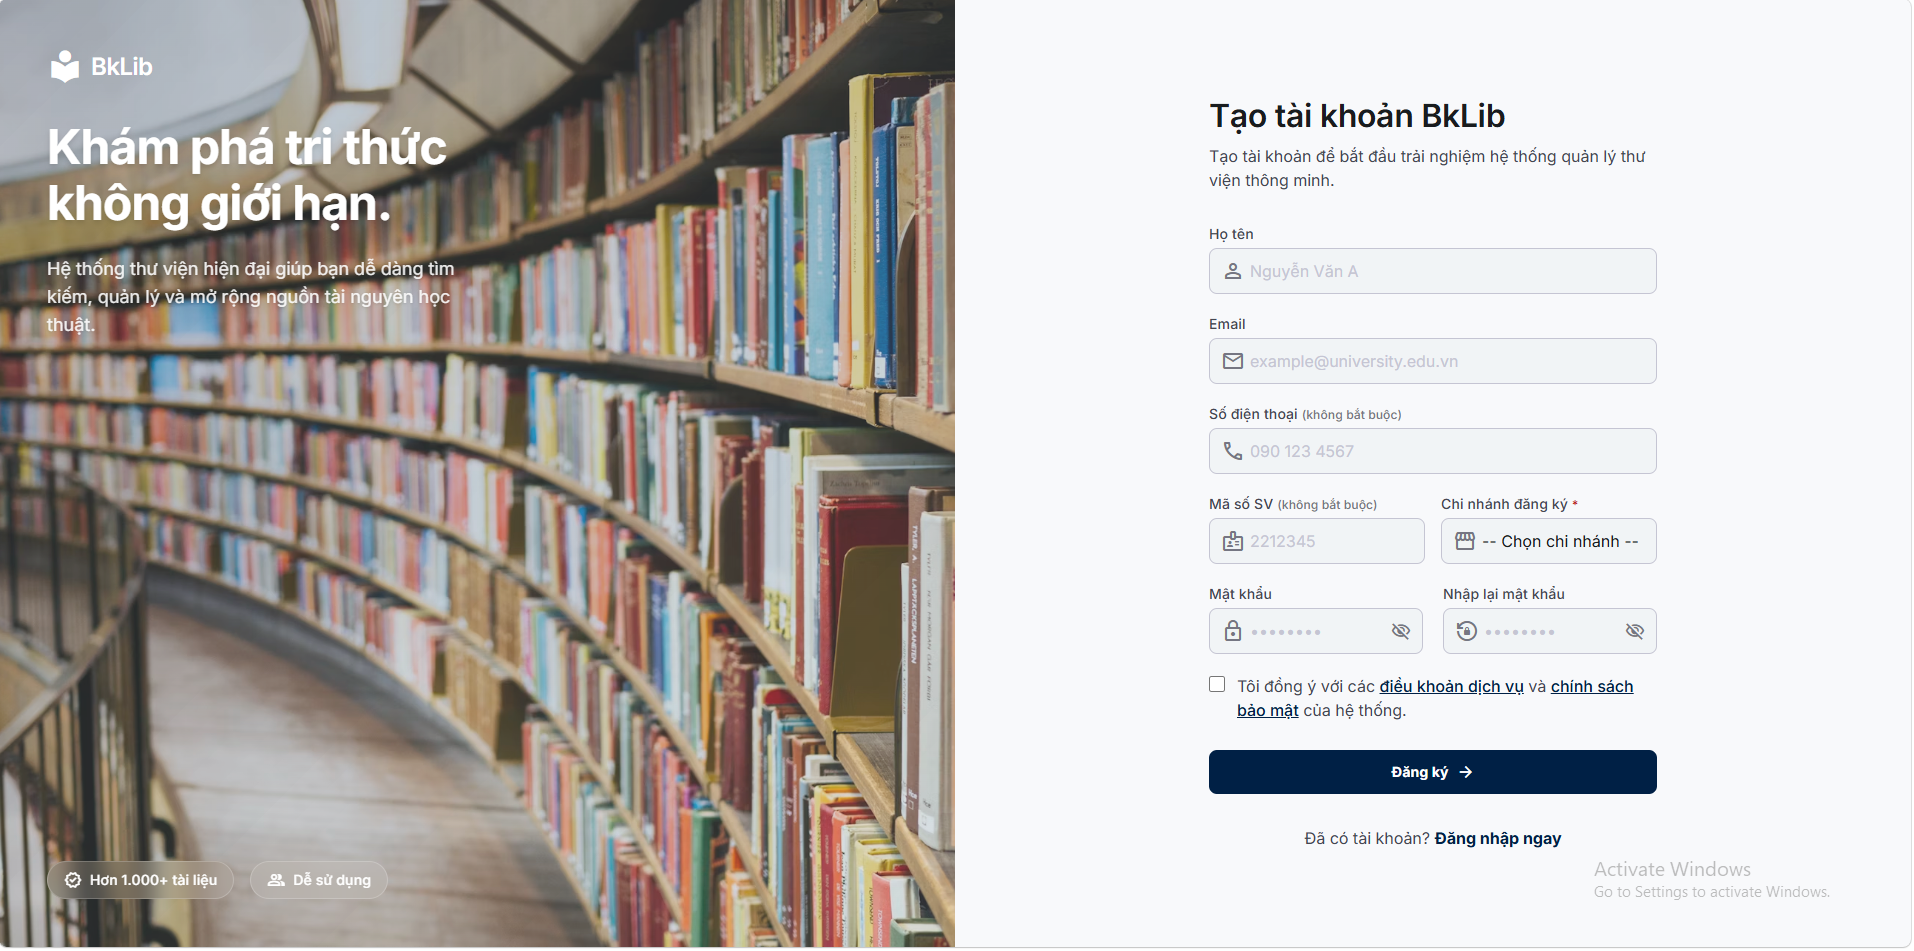
\includegraphics[width=0.95\linewidth]{Images/Auth_DangKy.png}
    \vspace{10pt}
    \caption{Giao diện Đăng ký Tài khoản BkLib}
    \label{fig:auth_register}
\end{figure}

\textbf{Bố cục \& Chức năng:} Biểu mẫu cấu trúc thu thập thông tin hồ sơ người dùng cơ bản, bao gồm Họ và Tên, Email, Số điện thoại (tùy chọn), Mã số Sinh viên ("Mã số SV" - tùy chọn) và Lựa chọn Chi nhánh ("Chi nhánh đăng ký"). Yêu cầu tạo mật khẩu với xác nhận khớp và đồng ý với điều khoản dịch vụ ("Điều khoản dịch vụ" và "Chính sách bảo mật") trước khi gửi yêu cầu đăng ký.

\paragraph{Quy trình Đặt lại Mật khẩu (Modal 3 bước)}
Cơ chế khôi phục mật khẩu tự phục vụ dạng modal sử dụng mã xác thực Email OTP 6 chữ số.

\begin{figure}[H]
    \centering
    \begin{subfigure}[b]{0.32\textwidth}
        \centering
        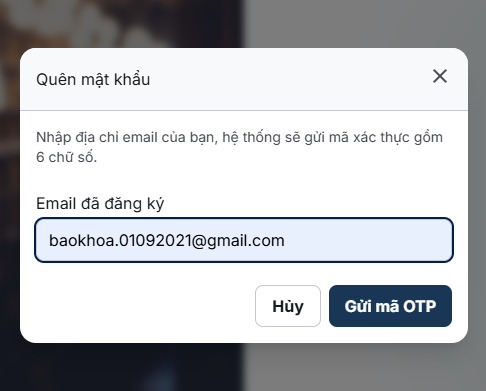
\includegraphics[width=\textwidth]{Images/Auth_QuenMatKhau_B1.png}
        \caption{Bước 1: Gửi Email}
        \label{fig:auth_reset_step1}
    \end{subfigure}
    \hfill
    \begin{subfigure}[b]{0.32\textwidth}
        \centering
        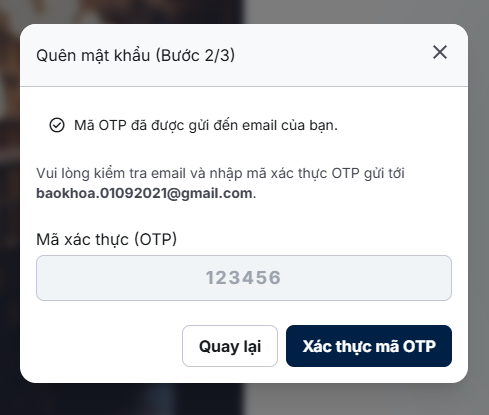
\includegraphics[width=\textwidth]{Images/Auth_QuenMatKhau_B2.png}
        \caption{Bước 2: Xác thực OTP}
        \label{fig:auth_reset_step2}
    \end{subfigure}
    \hfill
    \begin{subfigure}[b]{0.32\textwidth}
        \centering
        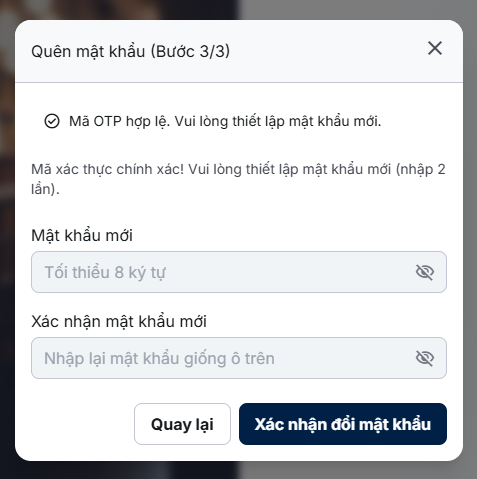
\includegraphics[width=\textwidth]{Images/Auth_QuenMatKhau_B3.png}
        \caption{Bước 3: Đặt lại Mật khẩu}
        \label{fig:auth_reset_step3}
    \end{subfigure}
    \vspace{10pt}
    \caption{Quy trình Modal 3 bước cho Khôi phục Mật khẩu}
    \label{fig:auth_forgot_password_flow}
\end{figure}

\textbf{Bố cục \& Chức năng:} Thực thi trong một hộp thoại modal đè lên gồm 3 giai đoạn tuần tự:
\begin{itemize}
    \item \textbf{Bước 1 (Yêu cầu OTP):} Người dùng nhập địa chỉ email đã đăng ký để hệ thống gửi mã xác thực 6 chữ số.
    \item \textbf{Bước 2 (Xác thực OTP):} Yêu cầu nhập mã 6 chữ số nhận được qua email, có phản hồi kiểm tra và nút quay lại.
    \item \textbf{Bước 3 (Cập nhật Mật khẩu):} Yêu cầu tạo và xác nhận mật khẩu mới (tối thiểu 8 ký tự) với biểu tượng con mắt để ẩn/hiện mật khẩu.
\end{itemize}

\subsubsection{Các Điểm sáng Hiện thực Kỹ thuật}

An ninh và bảo vệ các điểm cuối API được thực thi qua middleware sử dụng JSON Web Token (JWT) và hàm phân quyền vai trò bậc cao.

\begin{lstlisting}[caption={Middleware Xác thực và Phân quyền JWT (backend-express/src/middlewares/auth.middleware.ts)}, label={lst:auth_middleware}]
// Middleware verifing JWT access token from Authorization header
export const authenticate = (req: Request, res: Response, next: NextFunction): void => {
  const authHeader = req.headers.authorization;
  if (!authHeader || !authHeader.startsWith('Bearer ')) {
    res.status(401).json({ success: false, message: 'No authorization token provided' });
    return;
  }
  const token = authHeader.split(' ')[1];
  try {
    const decoded = jwt.verify(token, env.JWT_SECRET) as AuthPayload;
    req.user = decoded;
    next();
  } catch (err) {
    res.status(401).json({ success: false, message: 'Invalid or expired token' });
  }
};

// Middleware factory restricting access to specified roles
export const authorize = (...roles: Role[]) => {
  return (req: Request, res: Response, next: NextFunction): void => {
    if (!req.user || !roles.includes(req.user.role)) {
      res.status(403).json({ success: false, message: 'Access denied' });
      return;
    }
    next();
  };
};
\end{lstlisting}

% =========================================================================
% SECTION 5.3: READER MODULE
% =========================================================================
\subsection{Mô-đun Độc giả}

Mô-đun Độc giả cung cấp các khả năng tự phục vụ cho bạn đọc thư viện. Cho phép độc giả đã xác thực duyệt danh mục, thực hiện tìm kiếm bằng AI ngữ nghĩa, theo dõi và gia hạn lượt mượn, giám sát vị trí hàng chờ đặt chỗ, xem lịch sử giao dịch mượn trả và tương tác với widget trợ lý ảo.

\subsubsection{Hiện thực Giao diện Người dùng}

\paragraph{Trang chủ}
Bảng điều khiển trung tâm cá nhân hóa hiển thị sau khi độc giả đăng nhập, đóng vai trò là trung tâm vận hành cho các hoạt động của bạn đọc.

\begin{figure}[H]
    \centering
    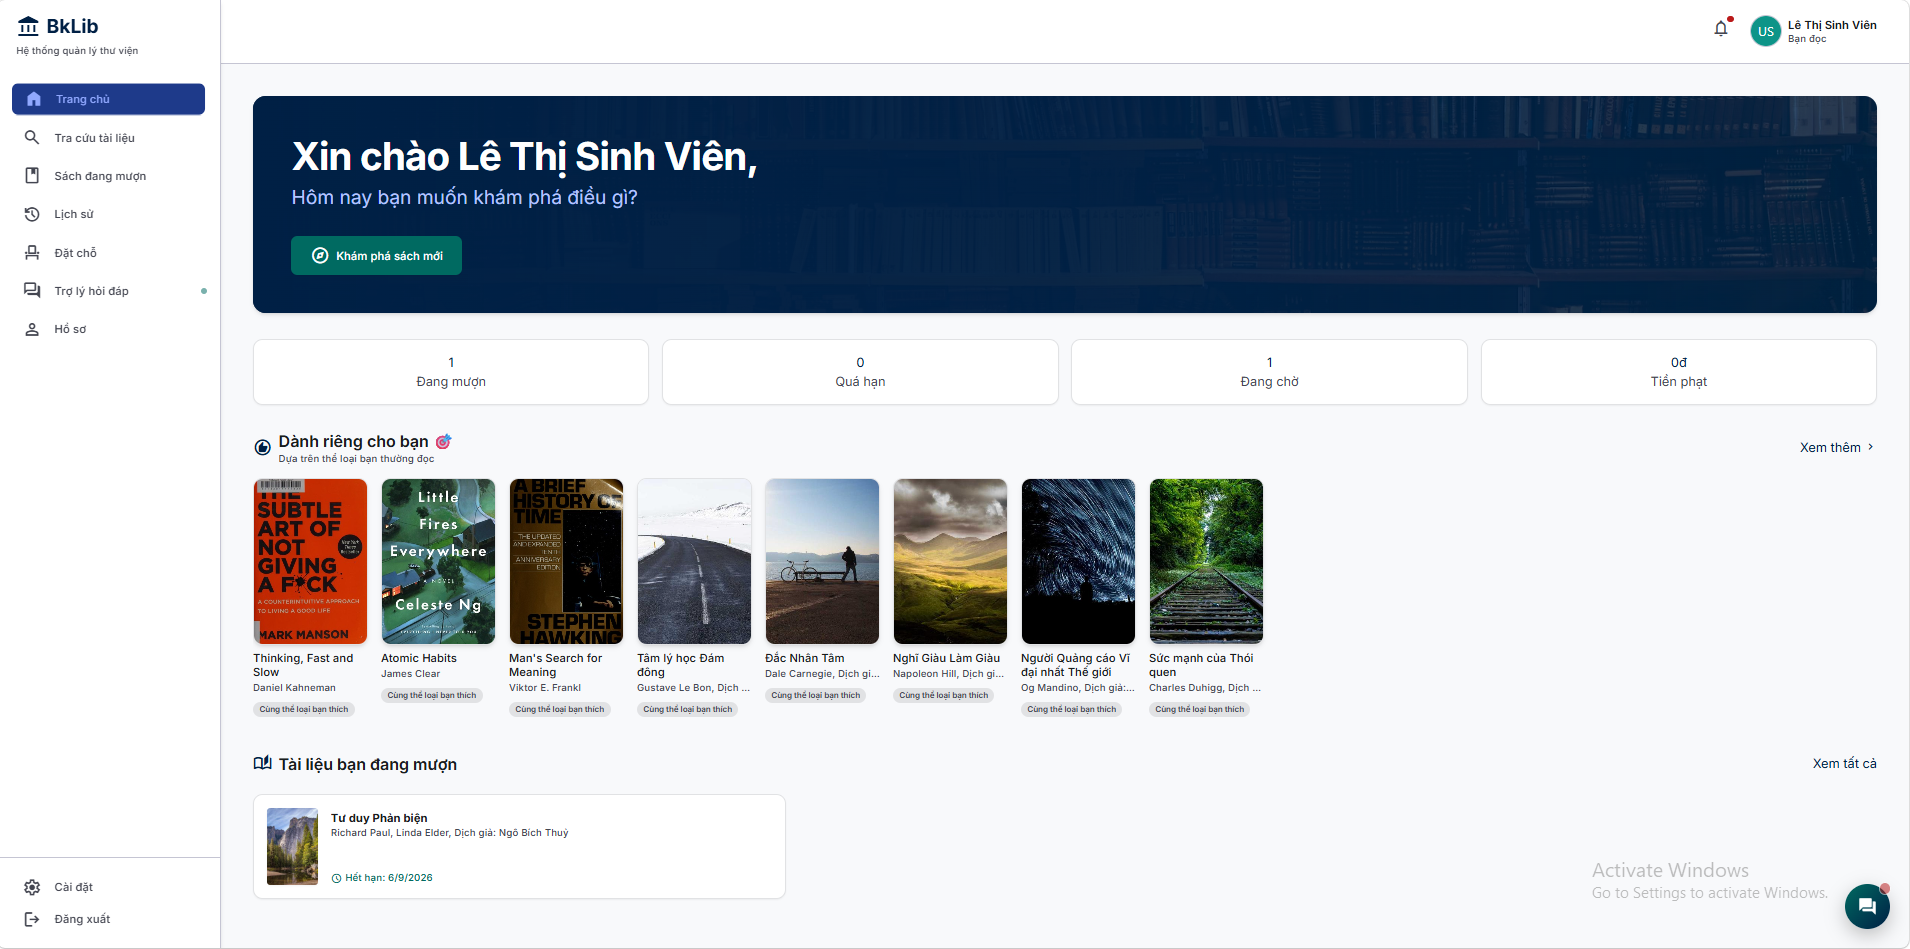
\includegraphics[width=0.95\linewidth]{Images/Reader_TrangChu.png}
    \vspace{10pt}
    \caption{Giao diện Trang chủ Mô-đun Độc giả}
    \label{fig:reader_homepage}
\end{figure}

\textbf{Bố cục \& Chức năng:} Bao gồm thanh điều hướng bên trái đáp ứng, trung tâm thông báo phía trên, các thẻ tóm tắt chỉ số chính (sách đang mượn, tài liệu quá hạn, số lượt đặt chỗ, số dư tiền phạt) và các thẻ truy cập nhanh cho các sách đang mượn với chỉ báo thời hạn trả theo thời gian thực.

\paragraph{Trang Tra cứu Danh mục}
Giao diện khám phá, lọc đa tiêu chí và duyệt danh mục tài nguyên thư viện.

\begin{figure}[H]
    \centering
    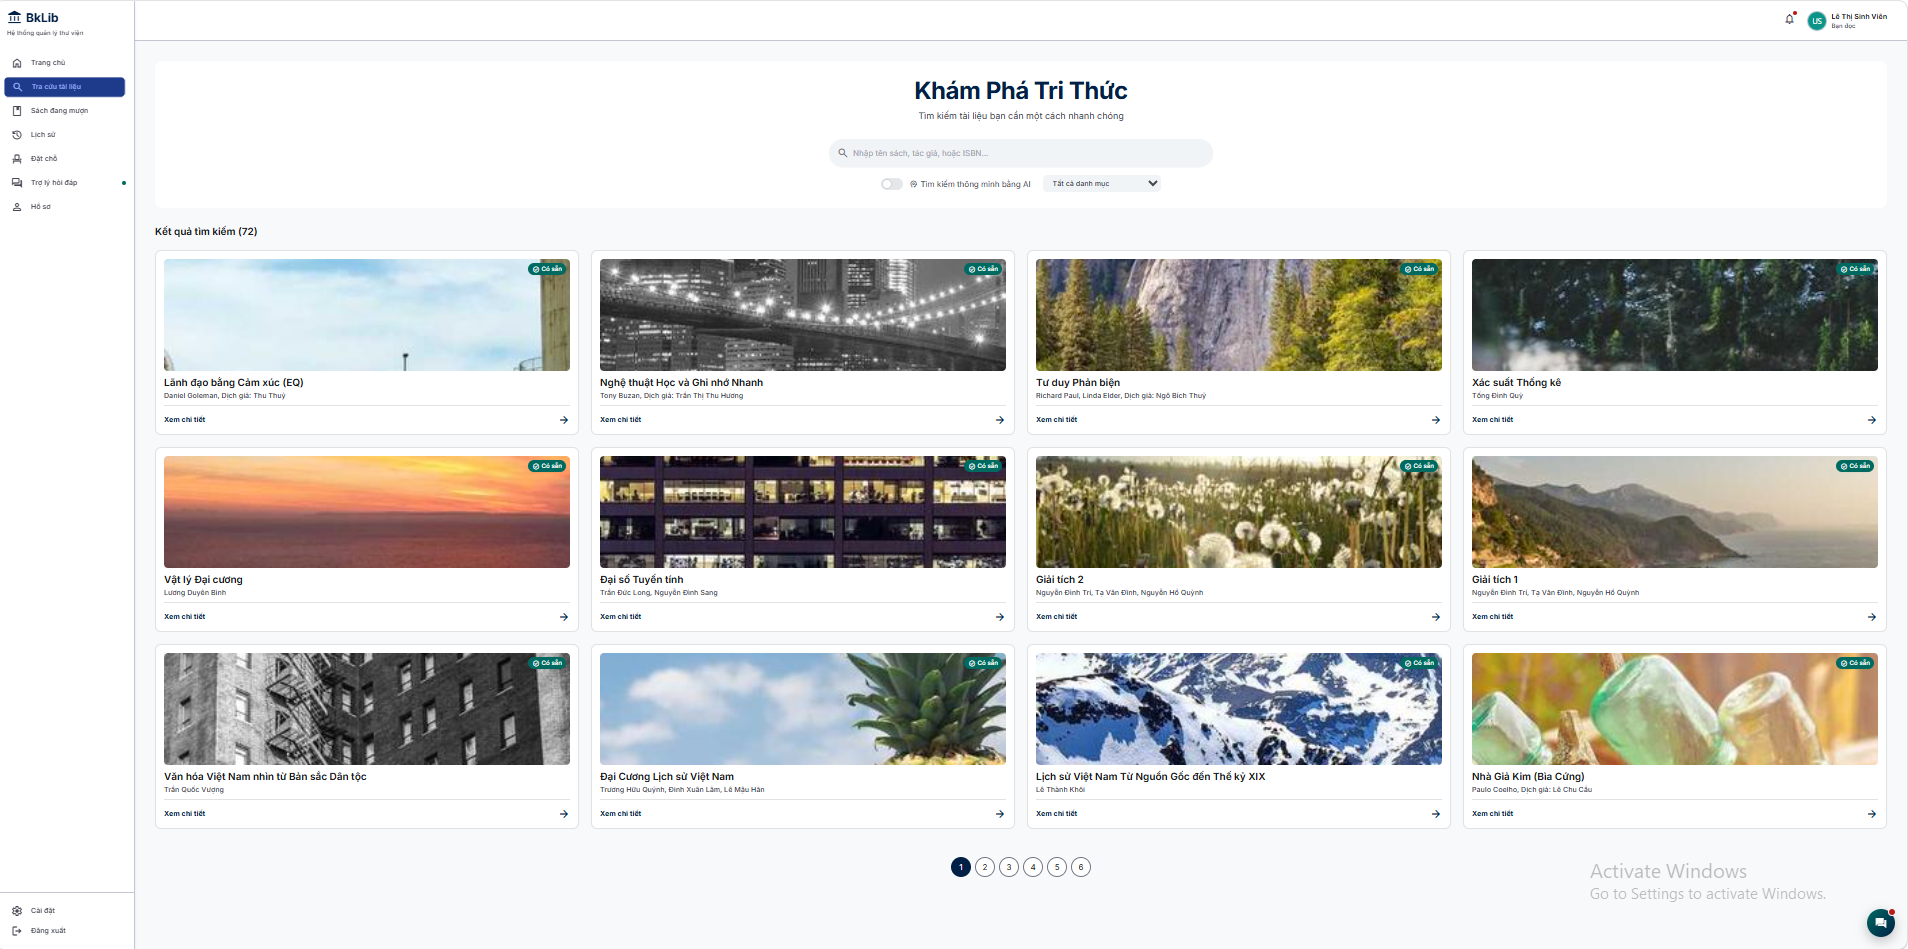
\includegraphics[width=0.95\linewidth]{Images/Reader_TraCuu.png}
    \vspace{10pt}
    \caption{Giao diện Tra cứu Danh mục}
    \label{fig:reader_search}
\end{figure}

\textbf{Bố cục \& Chức năng:} Tích hợp thanh tìm kiếm từ khóa nâng cao với bộ lọc thể loại và tính khả dụng theo chi nhánh. Độc giả có thể xem ảnh bìa, dữ liệu tả (tác giả, nhà xuất bản, ISBN), trạng thái khả dụng thực tế và thực hiện đặt chỗ trực tiếp từ các thẻ kết quả tìm kiếm.

\paragraph{Trang Quản lý Sách Đang Mượn}
Giao diện chuyên biệt cho phép độc giả theo dõi vòng đời lượt mượn và kích hoạt gia hạn mượn sách trực tuyến.

\begin{figure}[H]
    \centering
    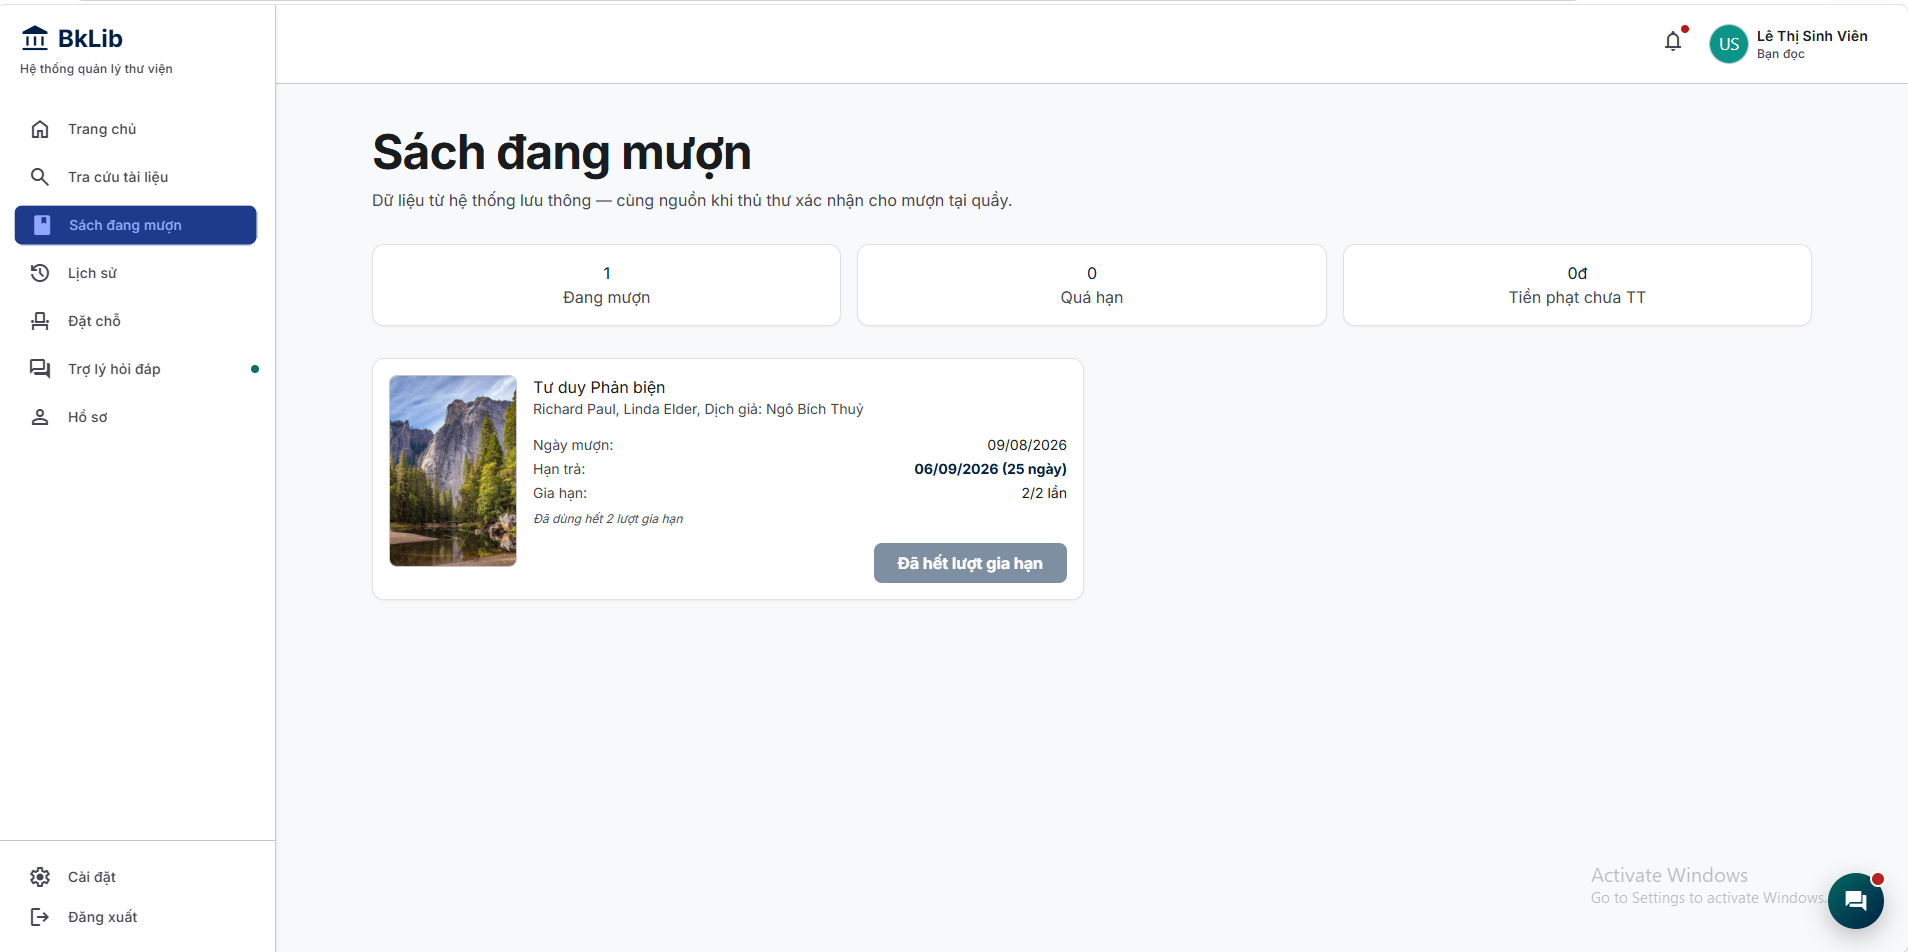
\includegraphics[width=0.95\linewidth]{Images/Reader_SachDangMuon.png}
    \vspace{10pt}
    \caption{Giao diện Quản lý Sách Đang Mượn}
    \label{fig:reader_borrowing}
\end{figure}

\textbf{Bố cục \& Chức năng:} Hiển thị thống kê tổng quan lượt mượn cùng các thẻ tài liệu chi tiết ghi rõ ngày mượn, hạn trả bắt buộc và số lần gia hạn cho phép. Độc giả có thể thực hiện gia hạn trực tiếp, hệ thống sẽ tự động truy vấn các quy tắc lưu thông để tính lại hạn trả hoặc cảnh báo rào cản gia hạn (như có người đặt chỗ hoặc đã đạt giới hạn gia hạn).

\paragraph{Trang Lịch sử Mượn Trả}
Sổ nhật ký lịch sử ghi lại các giao dịch trước đây, các tài liệu đã trả và giao dịch tài chính.

\begin{figure}[H]
    \centering
    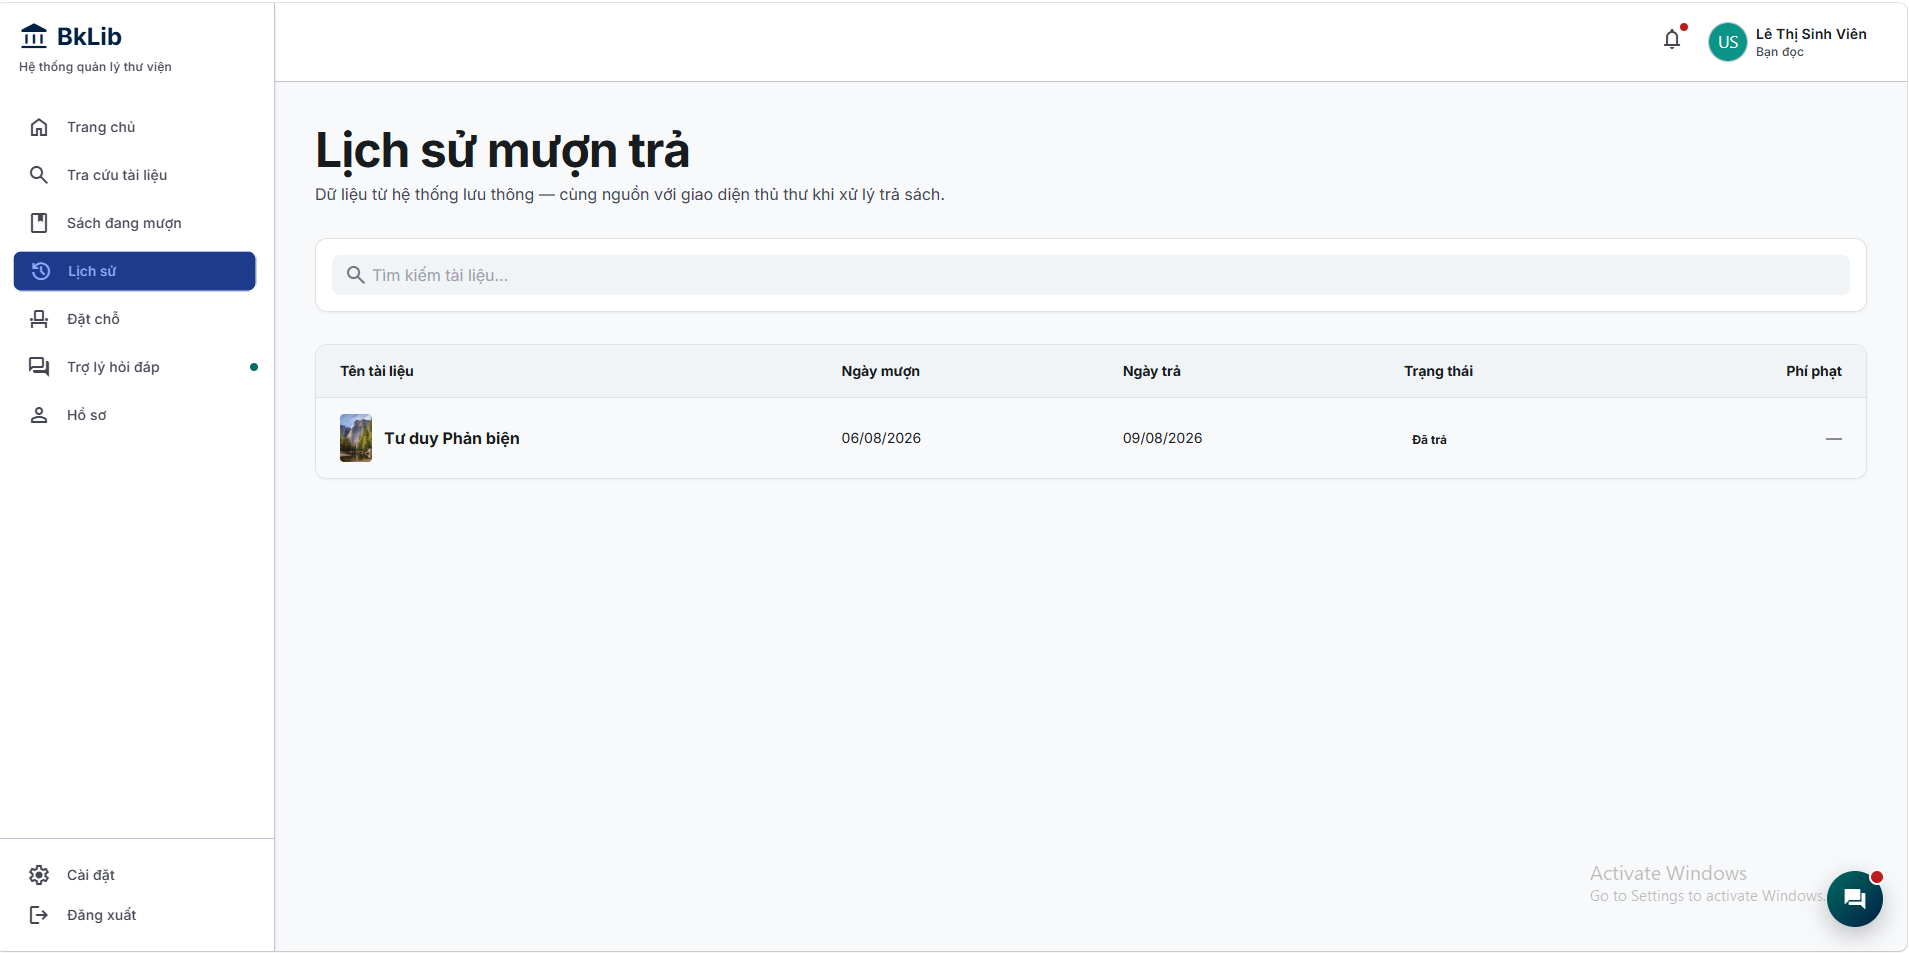
\includegraphics[width=0.95\linewidth]{Images/Reader_LichSu.png}
    \vspace{10pt}
    \caption{Giao diện Lịch sử Mượn Trả}
    \label{fig:reader_history}
\end{figure}

\textbf{Bố cục \& Chức năng:} Bảng cấu trúc chứa tên sách, ngày mượn, mốc thời gian trả thực tế, huy hiệu trạng thái hoàn thành và bản ghi tiền phạt. Hỗ trợ sắp xếp cột phía máy khách và bộ lọc theo khoảng thời gian để độc giả tự kiểm toán tài khoản.

\paragraph{Trang Quản lý Đặt Giữ Chỗ}
Theo dõi vị trí hàng chờ đặt chỗ và thông báo sách đã về cho các tài liệu đang hết hàng.

\begin{figure}[H]
    \centering
    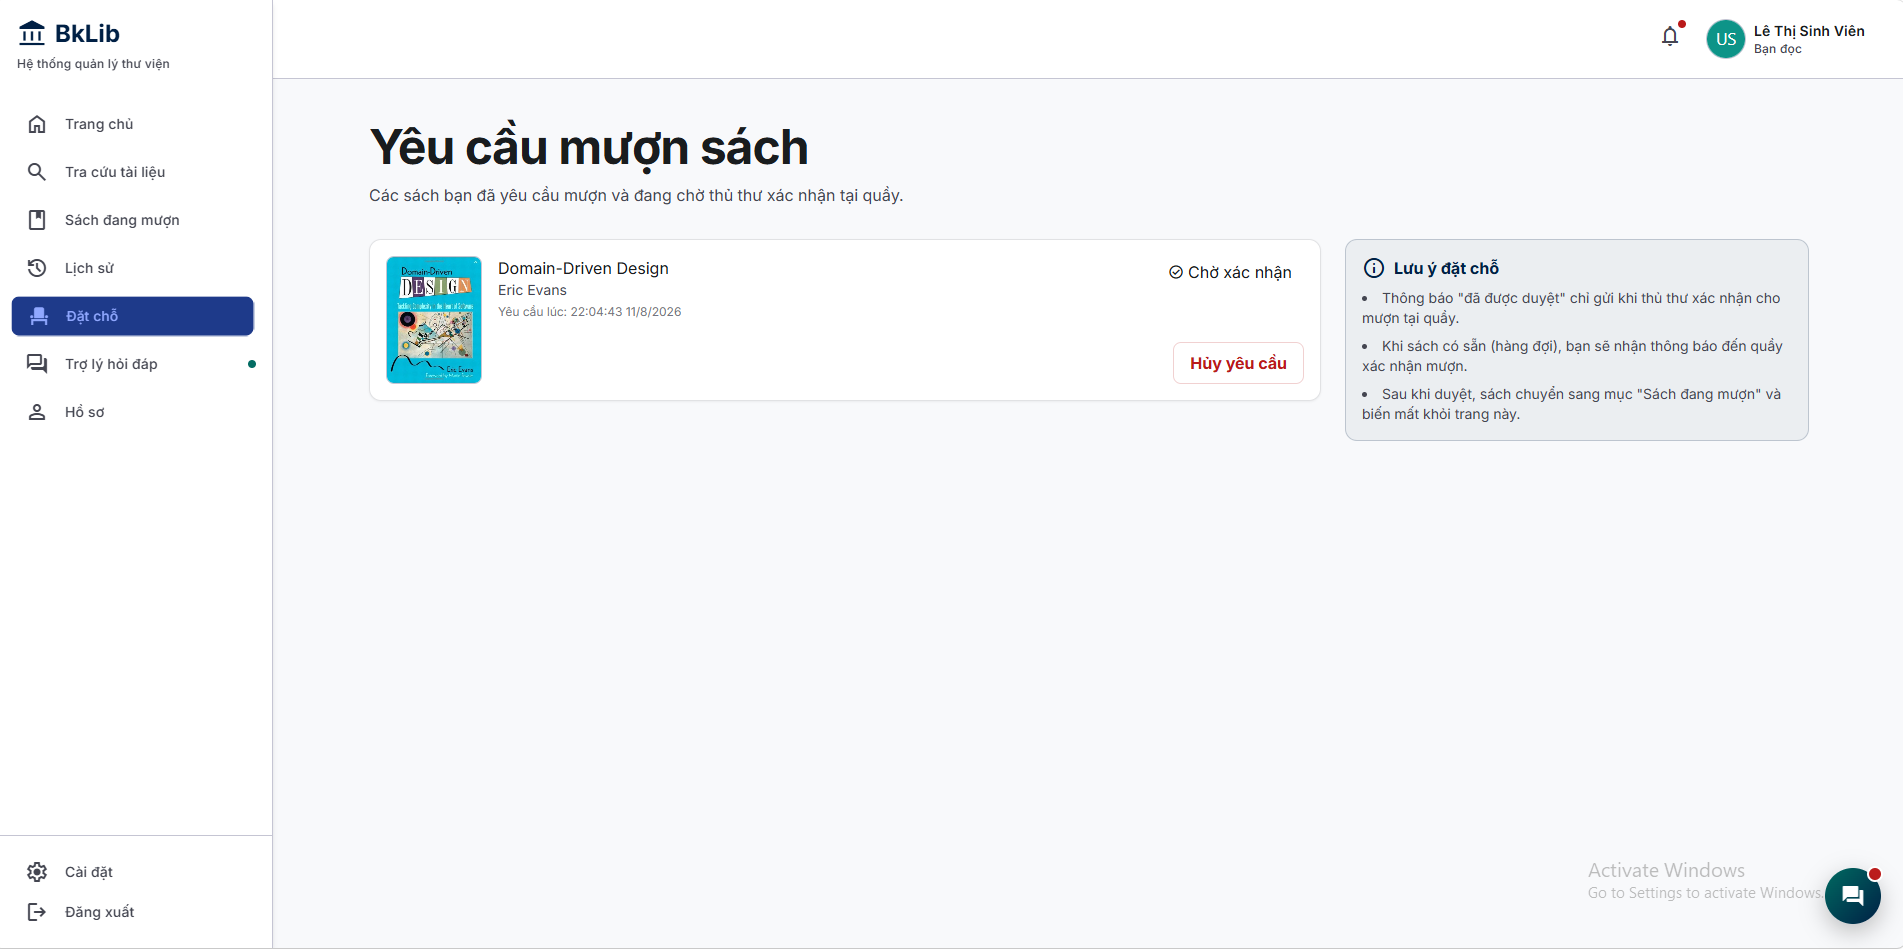
\includegraphics[width=0.95\linewidth]{Images/Reader_DatCho.png}
    \vspace{10pt}
    \caption{Giao diện Quản lý Đặt Giữ Chỗ}
    \label{fig:reader_reservation}
\end{figure}

\textbf{Bố cục \& Chức năng:} Liệt kê các lượt đặt chỗ đang hoạt động với thứ tự hàng chờ, khoảng thời gian chờ nhận sách cho các thông báo sẵn sàng lấy sách, nút hủy đặt chỗ và bảng hướng dẫn chi tiết về quy định đặt chỗ và thời hạn lấy sách của thư viện.

\paragraph{Cửa sổ Trò chuyện Trợ lý Ảo AI}
Widget trợ lý AI tương tác hỗ trợ giao tiếp ngôn ngữ tự nhiên, Q\&A và gợi ý ngữ nghĩa.

\begin{figure}[H]
    \centering
    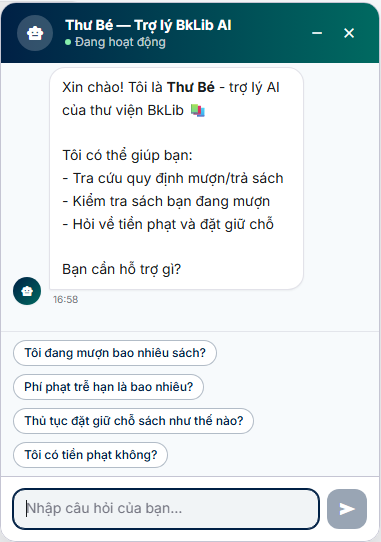
\includegraphics[width=0.45\linewidth]{Images/Reader_ChatbotAI.png}
    \vspace{10pt}
    \caption{Giao diện Cửa sổ Trò chuyện Trợ lý Ảo}
    \label{fig:reader_chatbot}
\end{figure}

\textbf{Bố cục \& Chức năng:} Giao diện trò chuyện nổi sử dụng backend RAG (Retrieval-Augmented Generation) kết hợp. Cung cấp các gợi ý câu hỏi, luồng tin nhắn phản hồi dạng streaming và các liên kết trực tiếp tới trang chi tiết sách được tạo từ các truy vấn tương đồng ngữ nghĩa.

\paragraph{Trang Hồ sơ Cá nhân \& Cài đặt}
Quản lý tài khoản độc giả, thông tin bảo mật và tùy chọn truyền thông.

\begin{figure}[H]
    \centering
    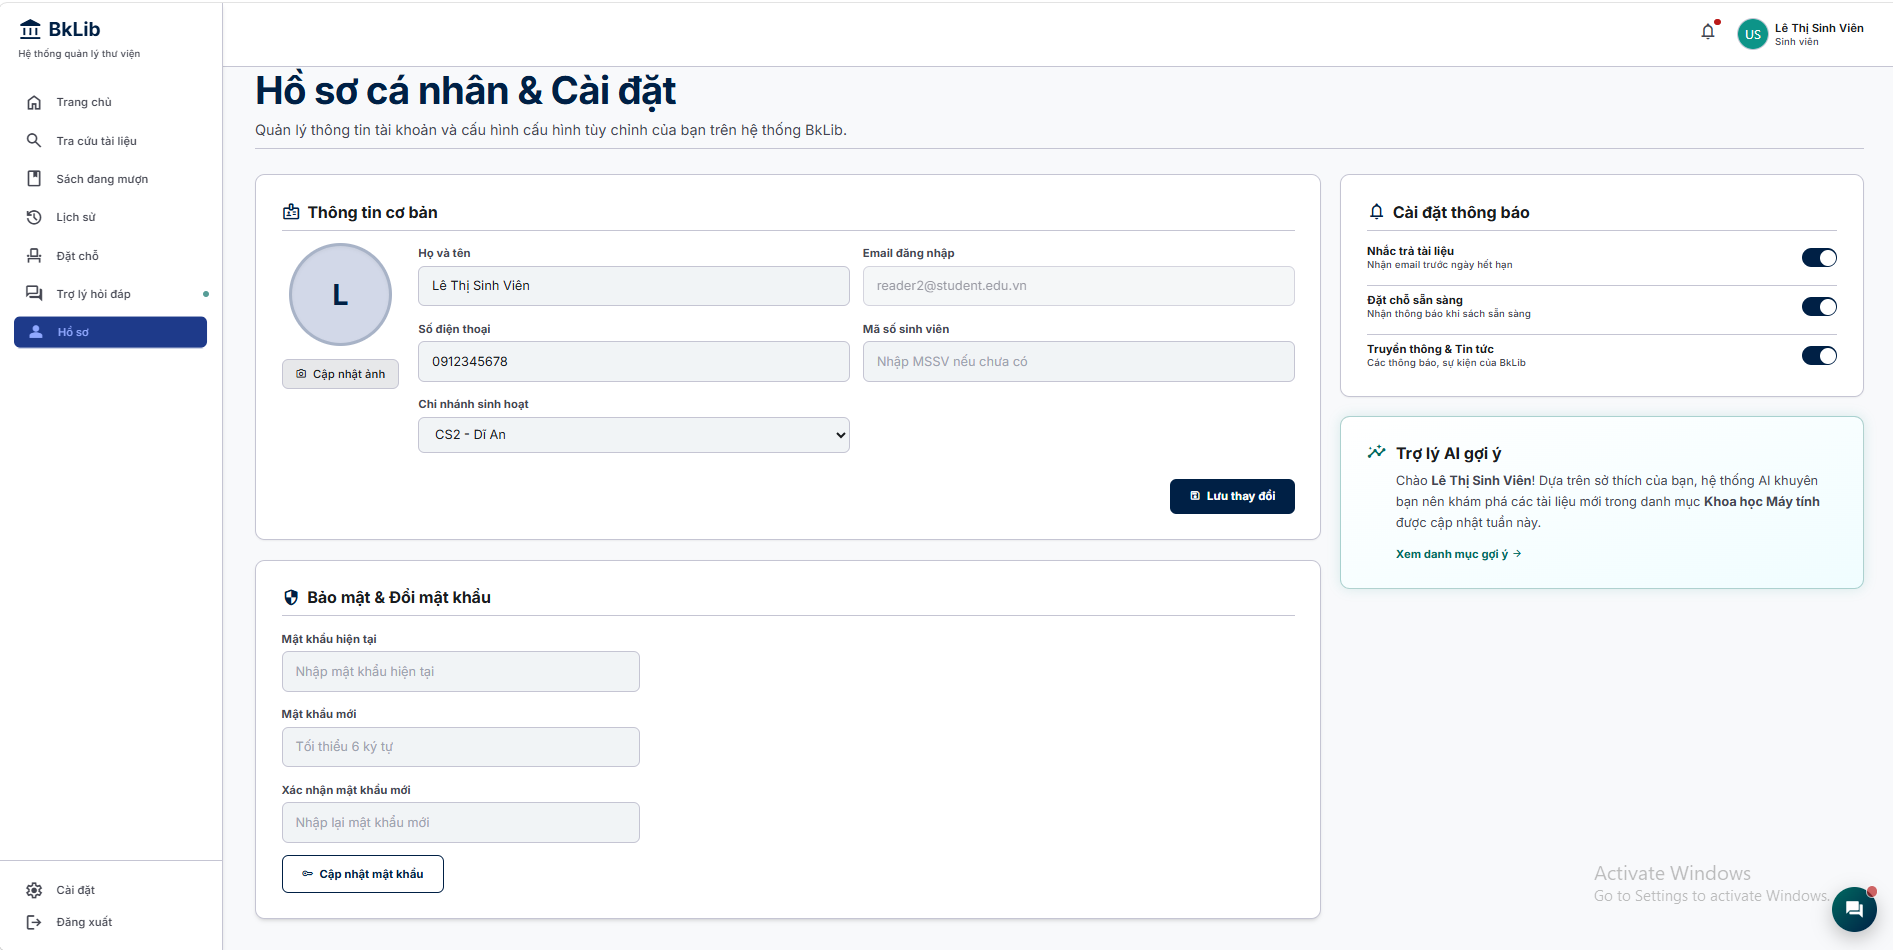
\includegraphics[width=0.95\linewidth]{Images/Reader_HoSoCaiDat.png}
    \vspace{10pt}
    \caption{Giao diện Hồ sơ Cá nhân và Cài đặt}
    \label{fig:reader_profile}
\end{figure}

\textbf{Bố cục \& Chức năng:} Chứa các biểu mẫu chỉnh sửa thông tin liên hệ, công cụ đổi mật khẩu, công tắc chuyển đổi kênh thông báo đa kênh (Email, SMS, In-App) và lưới gợi ý sách cá nhân hóa dựa trên lịch sử đọc của độc giả.

\subsubsection{Các Điểm sáng Hiện thực Kỹ thuật}

Trợ lý Ảo sử dụng các vector nhúng được tạo qua \texttt{SentenceTransformer} và lưu trữ trong bộ sưu tập \texttt{ChromaDB} để truy xuất các đoạn ngữ cảnh phù hợp nhất cho câu hỏi của độc giả.

\begin{lstlisting}[language=Python, caption={Truy xuất Vector ChromaDB cho RAG (ai-service/app/services/rag\_service.py)}, label={lst:rag_retrieval}]
def retrieve_context(query: str, top_k: int = 3) -> str:
    """
    Retrieve top-k relevant text chunks for a query from ChromaDB vector collection.
    Formats results with segment headers to feed into LLM prompt context.
    """
    if _collection is None or _collection.count() == 0:
        return ""

    embedder = get_embeddings()
    query_embedding = embedder.encode([query]).tolist()

    results = _collection.query(
        query_embeddings=query_embedding,
        n_results=min(top_k, _collection.count()),
    )
    docs = results.get("documents", [[]])[0]
    if not docs:
        return ""

    return "\n\n---\n\n".join([f"[Chunk {i+1}]: {doc}" for i, doc in enumerate(docs)])
\end{lstlisting}

% =========================================================================
% SECTION 5.4: LIBRARIAN MODULE
% =========================================================================
\subsection{Mô-đun Thủ thư}

Mô-đun Thủ thư hỗ trợ nhân viên thư viện thực hiện các hoạt động hằng ngày tại quầy, quản lý việc mượn trả tài liệu, duy trì dữ liệu tả danh mục, tính toán phí phạt, gửi thông báo hệ thống và phân tích hiệu suất chi nhánh.

\subsubsection{Hiện thực Giao diện Người dùng}

\paragraph{Trang chủ}
Bảng điều khiển vận hành làm nổi bật các nhiệm vụ hằng ngày, chỉ số trạng thái chi nhánh và hàng chờ xử lý khẩn cấp.

\begin{figure}[H]
    \centering
    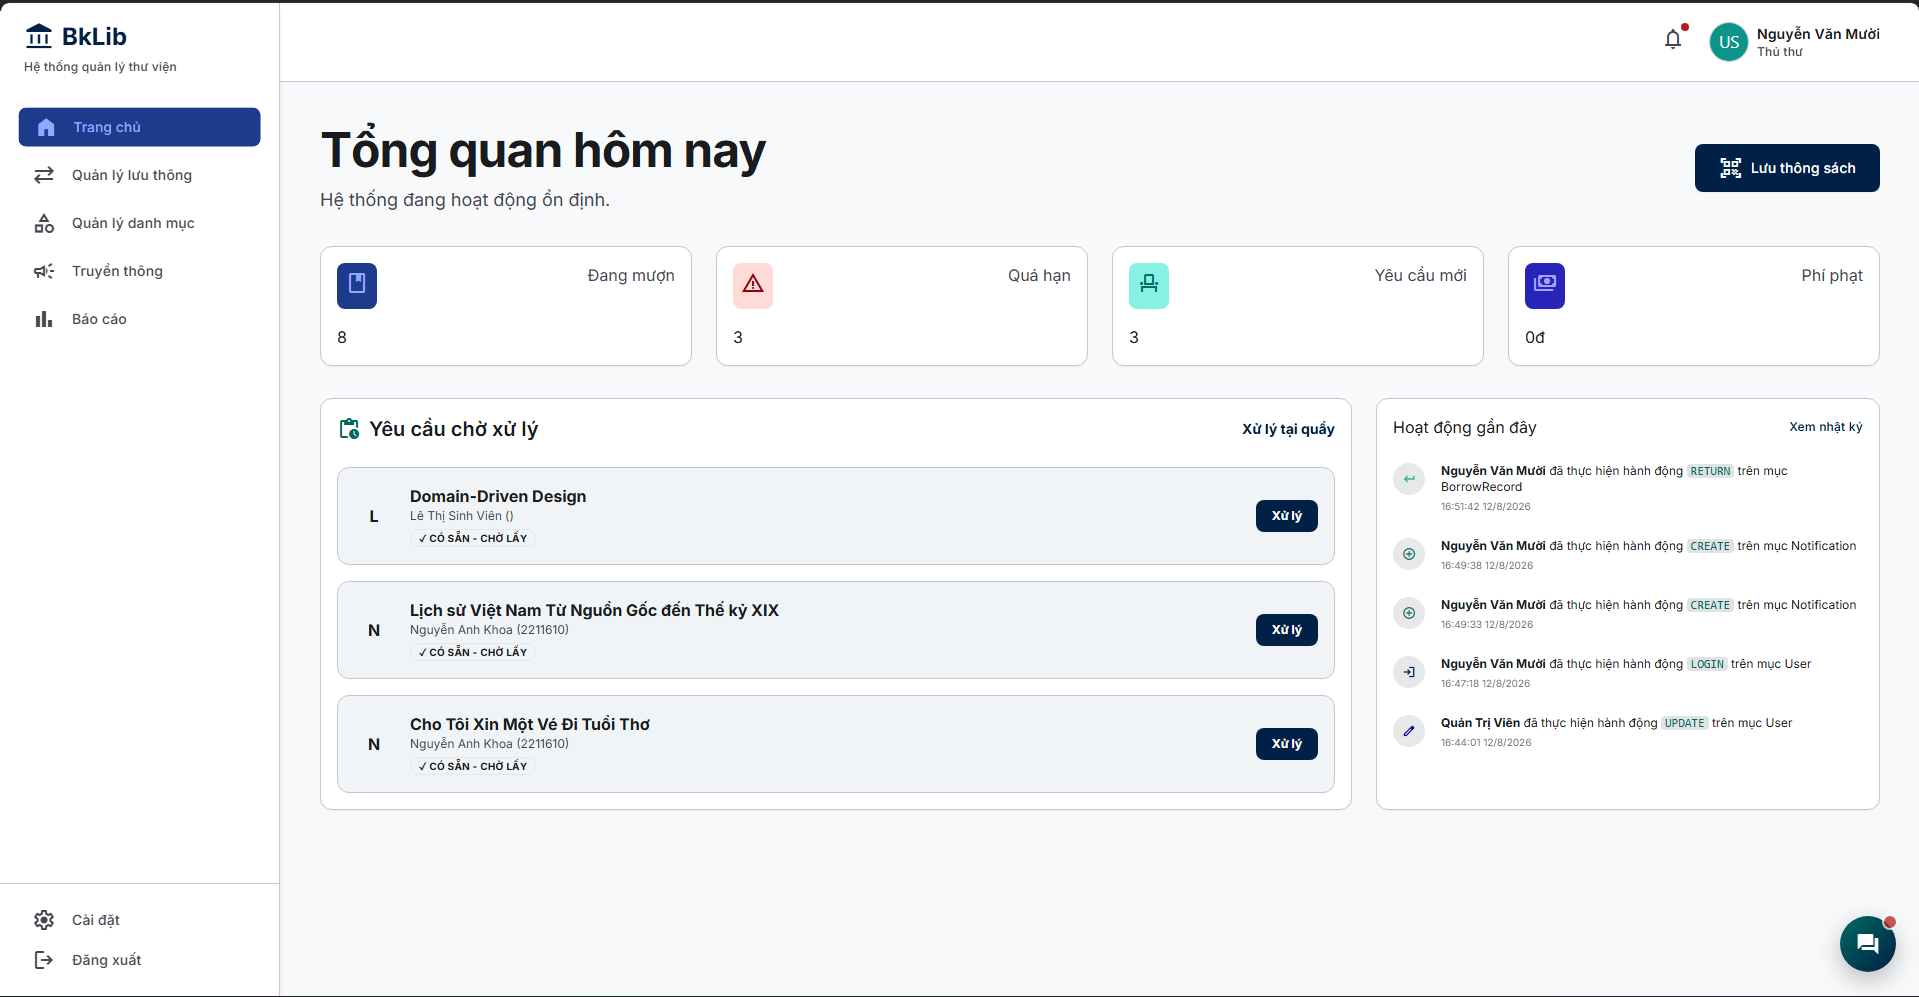
\includegraphics[width=0.95\linewidth]{Images/Librarian_TrangChu.png}
    \vspace{10pt}
    \caption{Giao diện Trang chủ Mô-đun Thủ thư}
    \label{fig:librarian_homepage}
\end{figure}

\textbf{Bố cục \& Chức năng:} Cung cấp các lối tắt truy cập nhanh (Lưu thông, Biên mục, Thông báo, Báo cáo), chỉ số hiệu suất quầy theo thời gian thực, hàng chờ đặt chỗ đang chờ xử lý và luồng nhật ký ghi lại các hoạt động mượn trả mới nhất.

\paragraph{Trang Quản lý Lưu thông}
Giao diện xử lý tại quầy được tối ưu hóa cho tốc độ mượn, trả và thanh toán tiền phạt cao.

\begin{figure}[H]
    \centering
    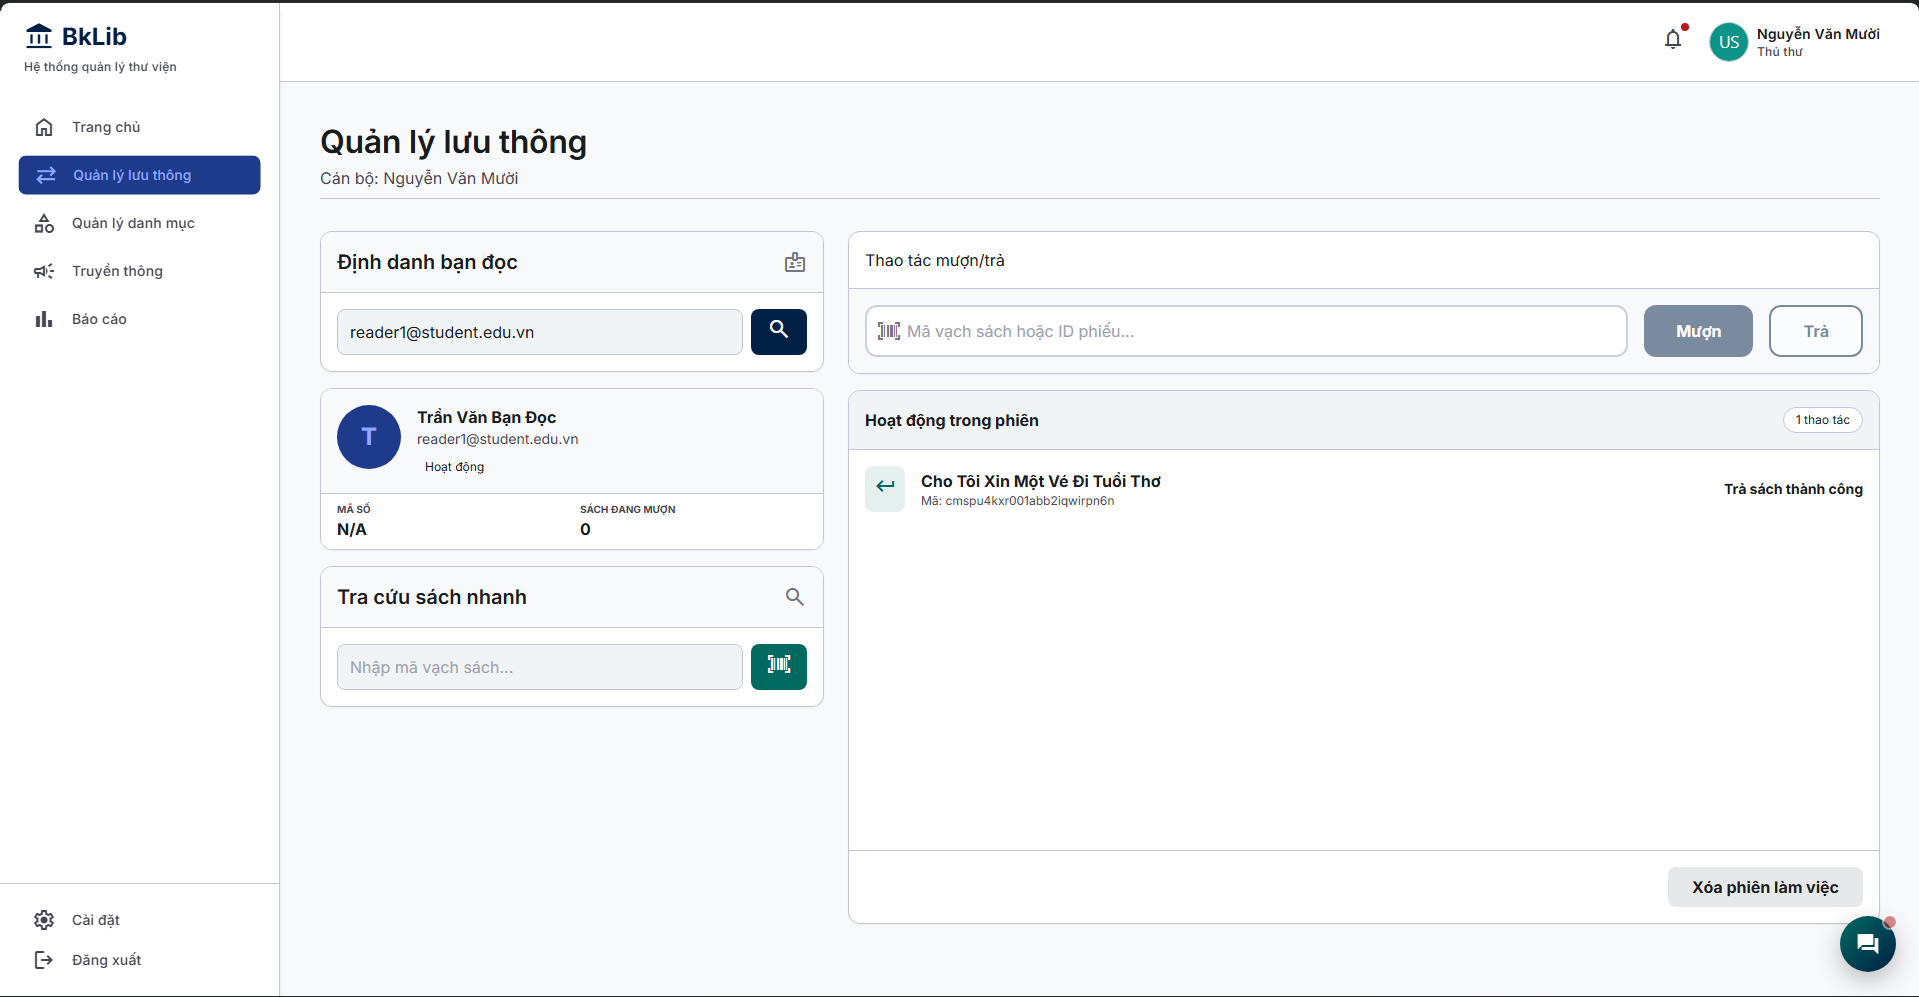
\includegraphics[width=0.95\linewidth]{Images/Librarian_QuanLyLuuThong.png}
    \vspace{10pt}
    \caption{Giao diện Quản lý Lưu thông}
    \label{fig:librarian_circulation}
\end{figure}

\textbf{Bố cục \& Chức năng:} Giao diện hai khung: khung tra cứu Thẻ/ID Độc giả bên trái, và ô quét mã vạch nhanh với tóm tắt giao dịch và xác minh trả sách bên phải. Ngay lập tức xác minh trạng thái tài khoản độc giả, các khoản giữ chỗ quá hạn và tự động tính tiền phạt khi quét mã.

\paragraph{Trang Quản lý Danh mục}
Không gian làm việc quản trị cho dữ liệu tả sách, theo dõi tồn kho và dán mã vạch bản sao vật lý.

\begin{figure}[H]
    \centering
    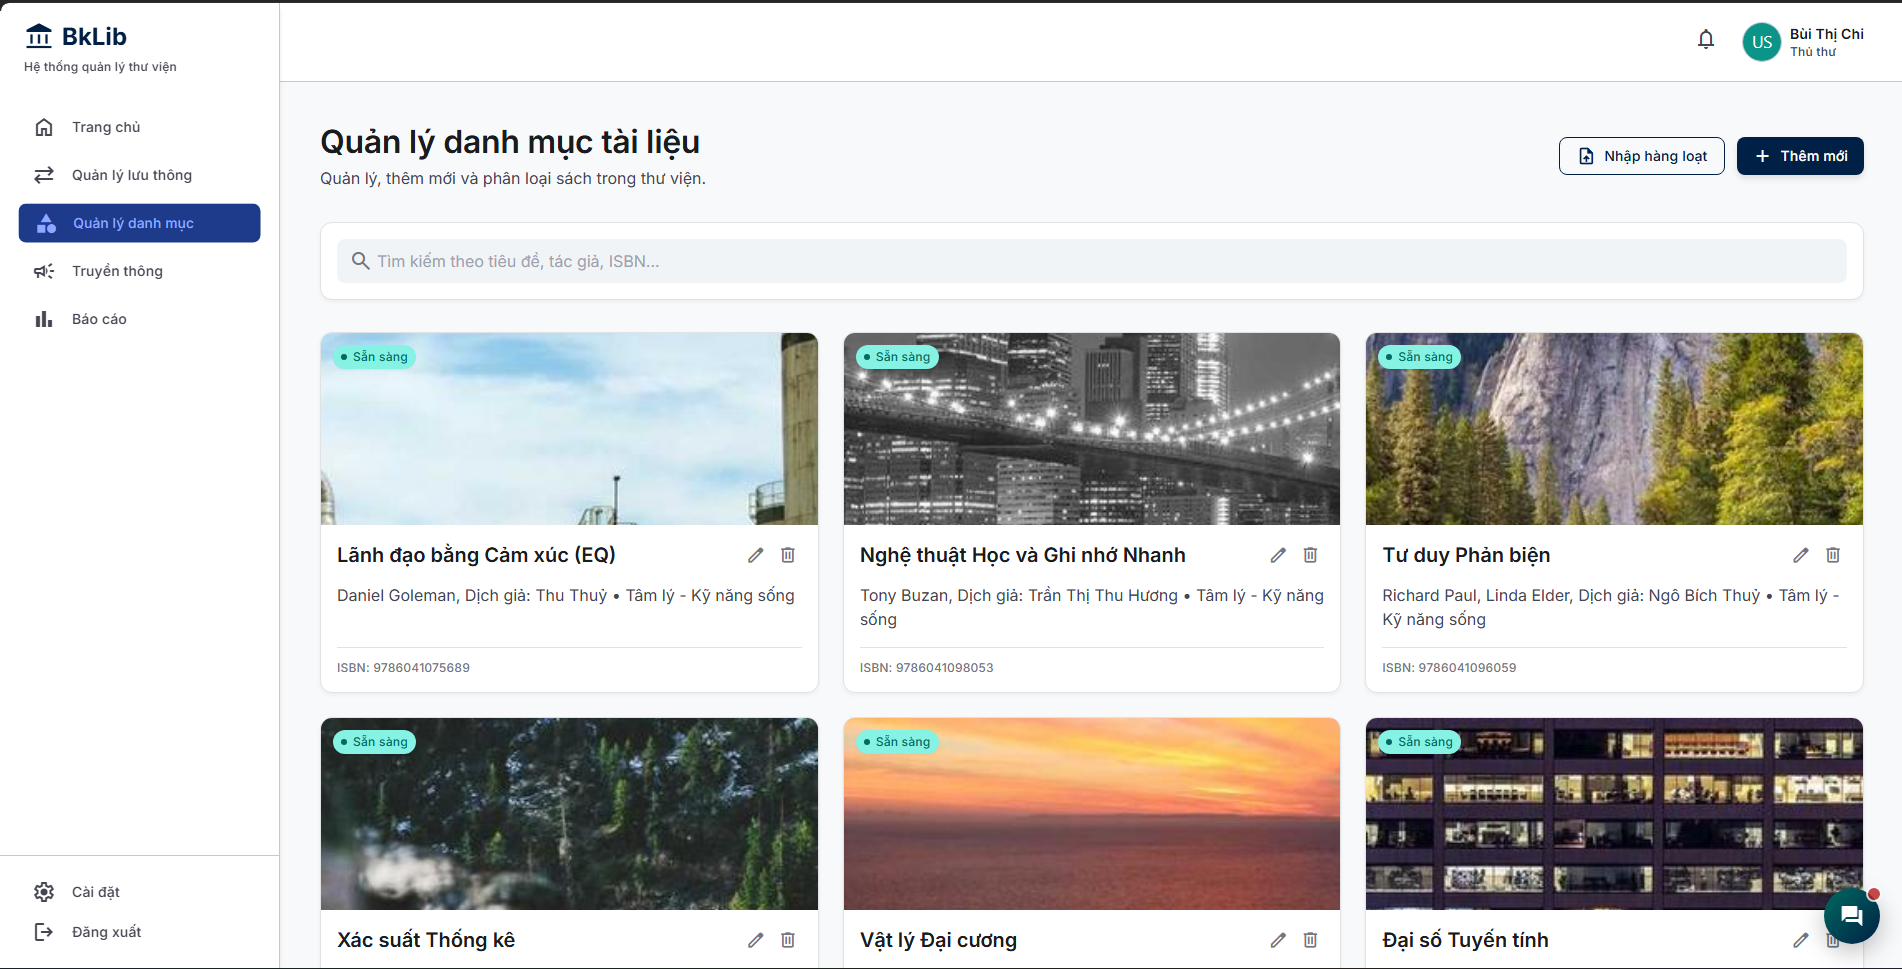
\includegraphics[width=0.95\linewidth]{Images/Librarian_QuanLyDanhMuc.png}
    \vspace{10pt}
    \caption{Giao diện Quản lý Danh mục}
    \label{fig:librarian_catalog}
\end{figure}

\textbf{Bố cục \& Chức năng:} Thanh công cụ tìm kiếm tích hợp tự động lấy dữ liệu qua ISBN, công cụ nhập dữ liệu hàng loạt từ CSV/Excel, biểu mẫu tạo tài liệu modal và bảng tồn kho phân trang hỗ trợ sửa trực tiếp, chuyển đổi trạng thái và tạo mã vạch bản sao.

\paragraph{Trang Quản lý Truyền thông}
Cổng phát thông báo cho các tin tức thư viện và chiến dịch thông báo tới nhóm độc giả mục tiêu.

\begin{figure}[H]
    \centering
    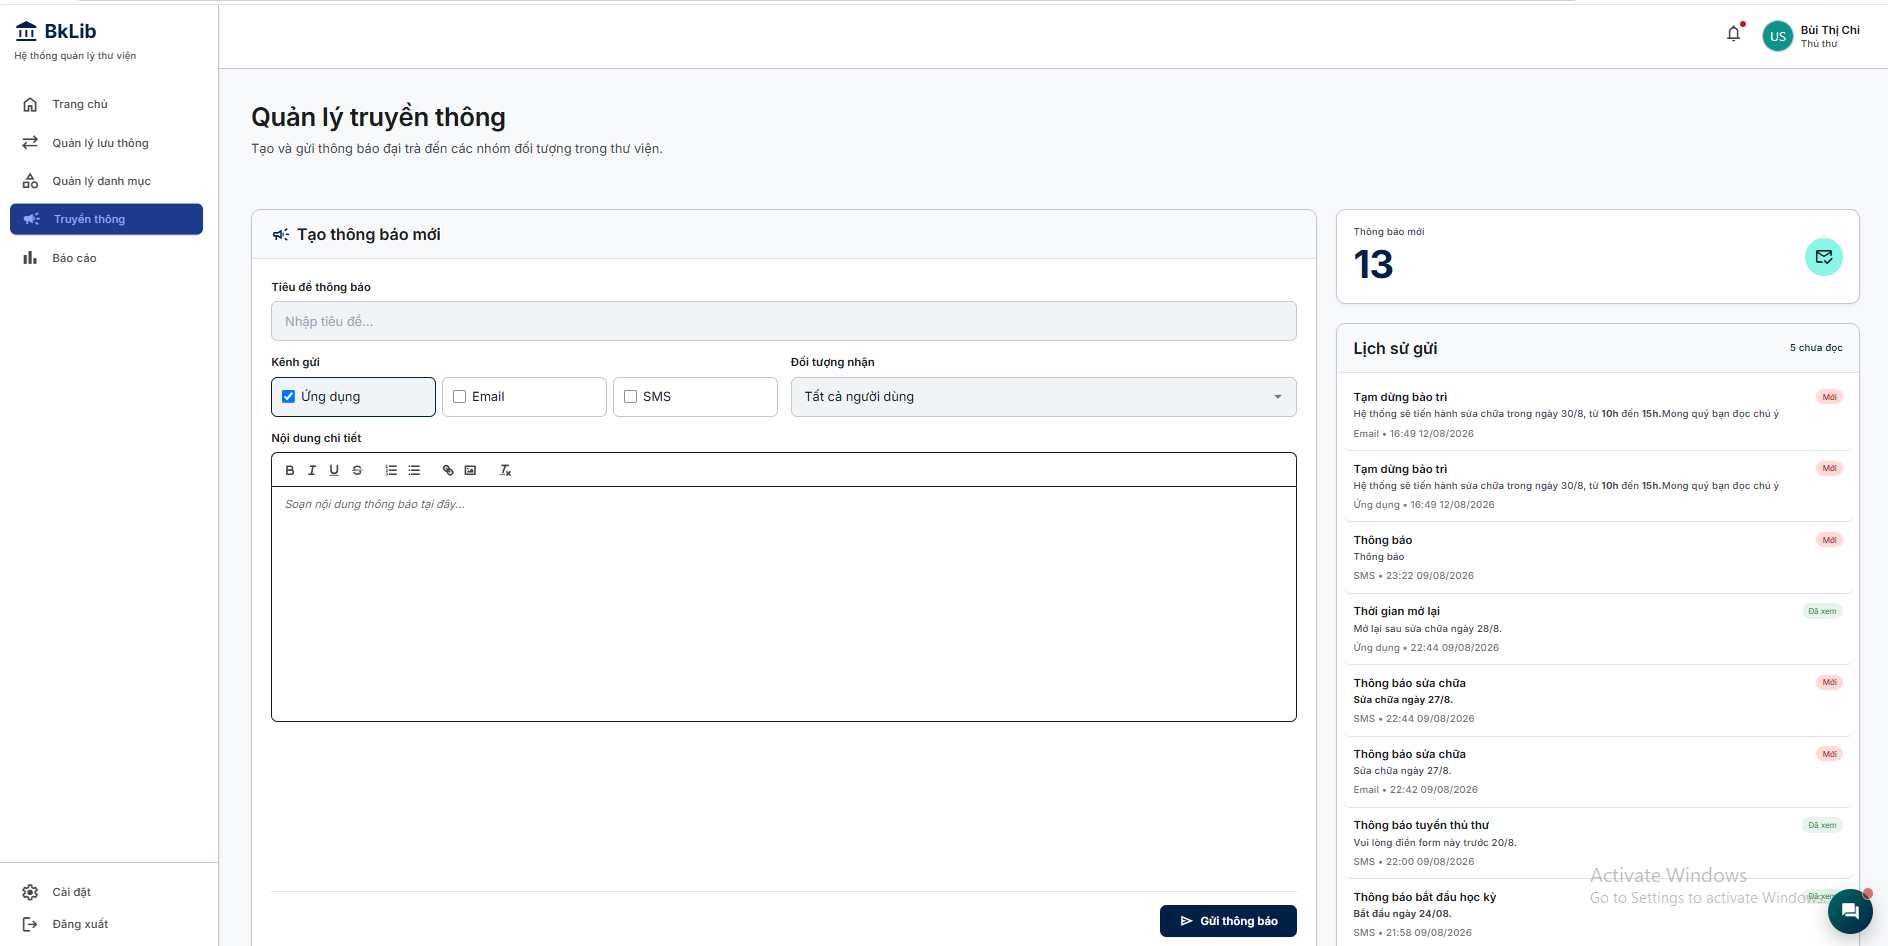
\includegraphics[width=0.95\linewidth]{Images/Librarian_TruyenThong.png}
    \vspace{10pt}
    \caption{Giao diện Quản lý Truyền thông}
    \label{fig:librarian_notification}
\end{figure}

\textbf{Bố cục \& Chức năng:} Trình soạn thảo thông báo văn bản giàu định dạng với tùy chọn chọn đối tượng đích (Tất cả độc giả, Độc giả quá hạn, Nhóm thành viên cụ thể), lựa chọn kênh (In-App, Email) và nhật ký lịch sử gửi ghi rõ tỷ lệ thành công.

\paragraph{Trang Báo cáo \& Phân tích}
Bảng điều khiển trực quan hóa dữ liệu theo dõi lưu lượng lưu thông, mức độ sử dụng bộ sưu tập và chỉ số tài chính.

\begin{figure}[H]
    \centering
    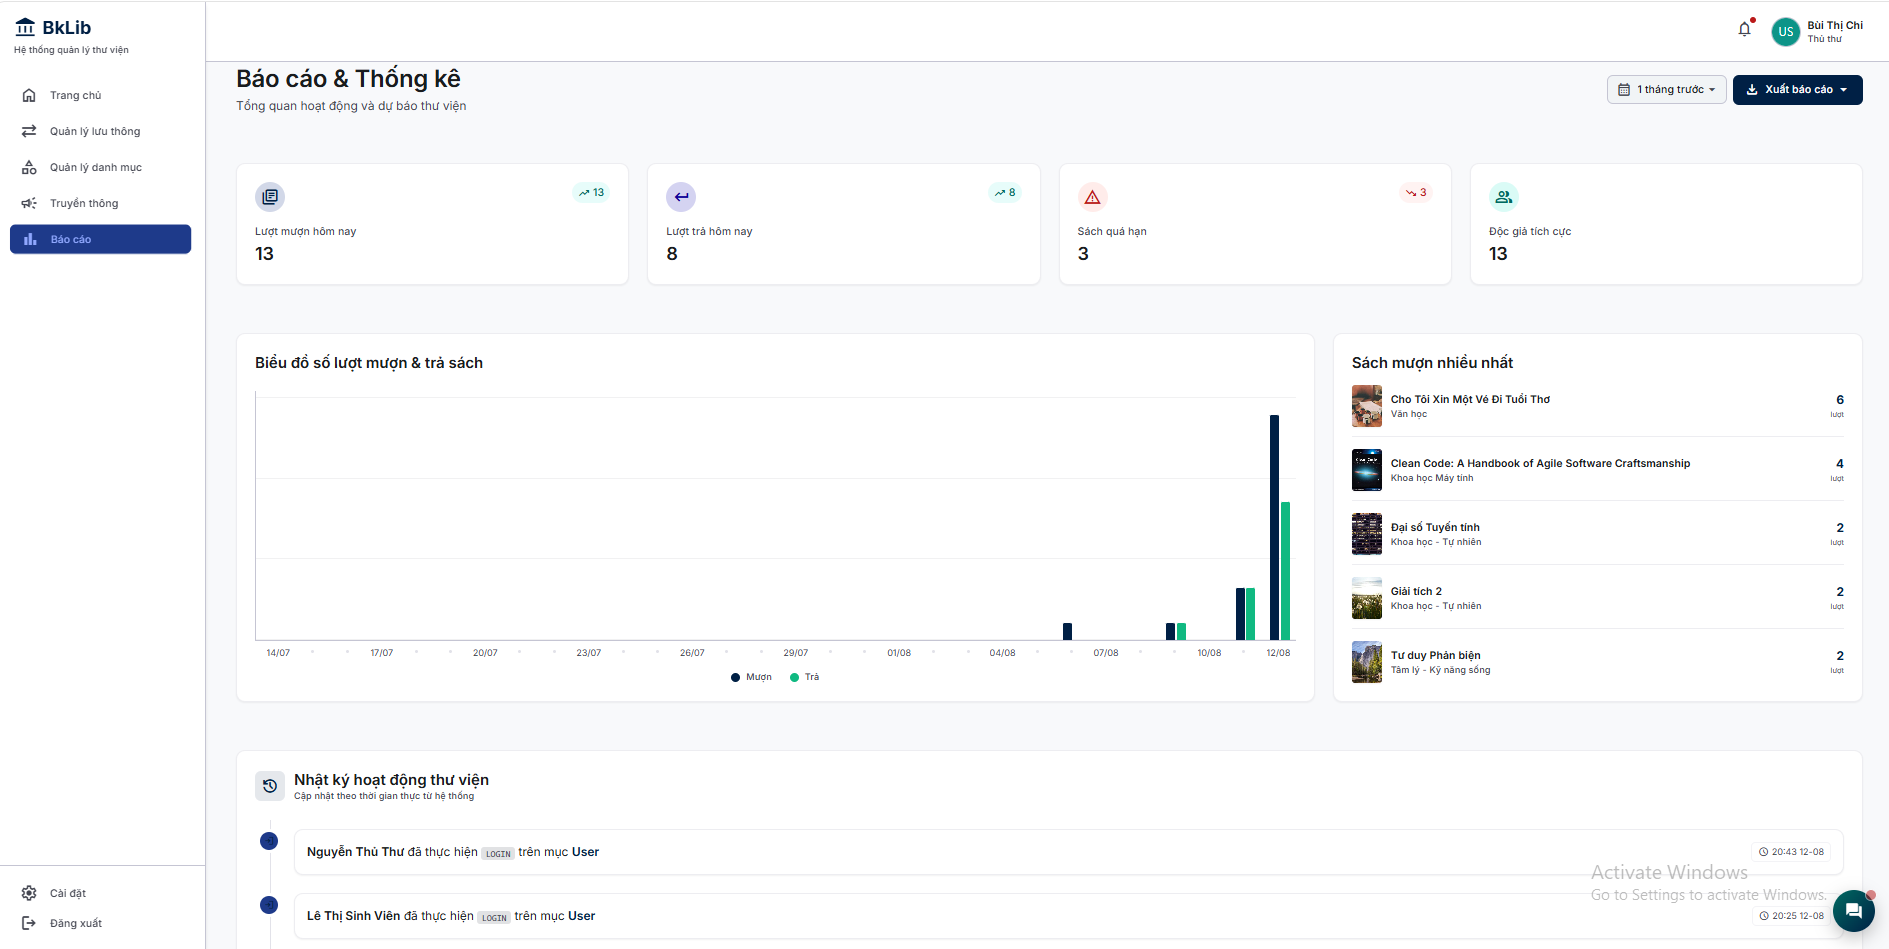
\includegraphics[width=0.95\linewidth]{Images/Librarian_BaoCao.png}
    \vspace{10pt}
    \caption{Giao diện Báo cáo và Phân tích cho Thủ thư}
    \label{fig:librarian_report}
\end{figure}

\textbf{Bố cục \& Chức năng:} Bộ điều khiển khoảng thời gian tương tác, nút xuất dữ liệu (PDF, Excel, CSV), biểu đồ xu hướng lưu thông, xếp hạng sách mượn nhiều nhất và phân tích thu tiền phạt để hỗ trợ kế hoạch bổ sung tài nguyên.

\paragraph{Trang Hồ sơ Cá nhân \& Cài đặt}
Không gian làm việc quản lý tài khoản nhân viên để cập nhật thuộc tính hồ sơ, mật khẩu bảo mật và tùy chọn nhận thông báo.

\begin{figure}[H]
    \centering
    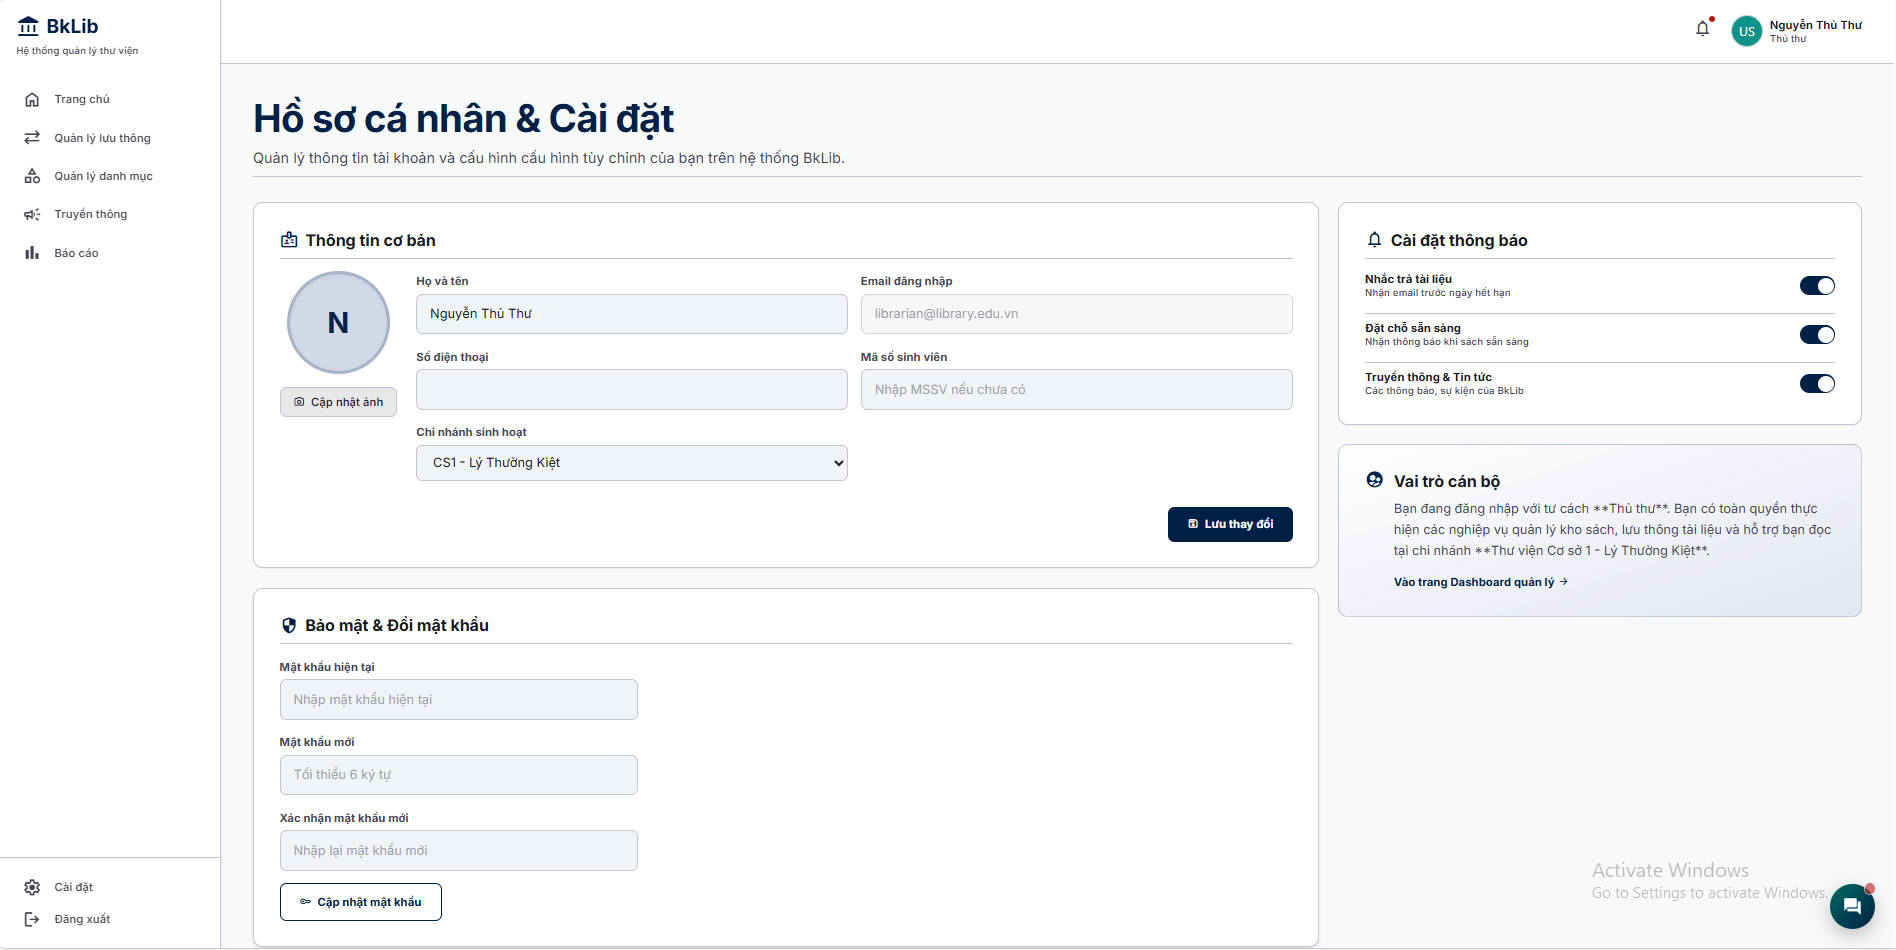
\includegraphics[width=0.95\linewidth]{Images/Librarian_HoSoCaiDat.png}
    \vspace{10pt}
    \caption{Giao diện Hồ sơ Cá nhân và Cài đặt Thủ thư}
    \label{fig:librarian_profile}
\end{figure}

\textbf{Bố cục \& Chức năng:} Được tổ chức thành bố cục bảng điều khiển nhiều thẻ:
\begin{itemize}
    \item \textbf{Khung Thông tin Cơ bản ("Thông tin cơ bản"):} Các trường hồ sơ có thể chỉnh sửa bao gồm họ tên, email đăng nhập, số điện thoại liên hệ, mã cán bộ, bộ chọn chi nhánh làm việc (ví dụ: CS1 - Lý Thường Kiệt) và công cụ cập nhật ảnh đại diện.
    \item \textbf{Bảo mật \& Đổi Mật khẩu ("Bảo mật \& Đổi mật khẩu"):} Công cụ quản lý mật khẩu yêu cầu xác nhận mật khẩu hiện tại trước khi nhập mật khẩu mới.
    \item \textbf{Tùy chọn Thông báo ("Cài đặt thông báo"):} Các công tắc bật/tắt cho các cảnh báo tự động, bao gồm nhắc nhở trả sách, thông báo đặt chỗ đã về và thông báo toàn hệ thống.
    \item \textbf{Tóm tắt Vai trò Cán bộ ("Vai trò cán bộ"):} Thẻ hiển thị các quyền hạn hiện tại, chi nhánh làm việc được phân công và liên kết trực tiếp tới bảng điều khiển quản trị.
\end{itemize}

\subsubsection{Các Điểm sáng Hiện thực Kỹ thuật}

Logic lưu thông tính toán động số ngày quá hạn bằng cách lặp qua các khoảng thời gian mượn trả đồng thời loại trừ các ngày nghỉ lễ chính thức của thư viện được cấu hình trong cài đặt hệ thống.

\begin{lstlisting}[caption={Tính số Ngày Quá hạn có Nhận biết Ngày Lễ (backend-express/src/modules/circulation/circulation.service.ts)}, label={lst:calc_overdue}]
const calcOverdueDays = async (dueDate: Date, returnDate: Date): Promise<number> => {
  if (returnDate <= dueDate) return 0;

  // Retrieve holiday array from system configuration
  const holidayConfig = await getConfig(CONFIG_KEYS.HOLIDAY_DATES, '[]');
  const holidays: string[] = JSON.parse(holidayConfig);

  let overdueDays = 0;
  const cursor = new Date(dueDate);
  cursor.setDate(cursor.getDate() + 1);

  // Iterate day-by-day excluding scheduled holidays
  while (cursor <= returnDate) {
    const dateStr = cursor.toISOString().split('T')[0];
    if (!holidays.includes(dateStr)) {
      overdueDays++;
    }
    cursor.setDate(cursor.getDate() + 1);
  }
  return overdueDays;
};
\end{lstlisting}

% =========================================================================
% SECTION 5.5: ADMINISTRATOR MODULE
% =========================================================================
\subsection{Mô-đun Quản trị viên}

Mô-đun Quản trị viên cung cấp khả năng quản trị cấp cao nhất cho nền tảng. Cho phép quản trị viên quản lý Kiểm soát Truy cập Dựa trên Vai trò (RBAC), cấu hình thiết lập hệ thống, quản lý mạng lưới chi nhánh, kiểm toán nhật ký hệ thống, giám sát sức khỏe hạ tầng và thực hiện các thao tác sao lưu, khôi phục cơ sở dữ liệu khi có sự cố.

\subsubsection{Hiện thực Giao diện Người dùng}

\paragraph{Bảng điều khiển Tổng quan Hệ thống}
Bảng điều khiển giám sát hạ tầng, tải máy chủ và thống kê sử dụng cấp cao.

\begin{figure}[H]
    \centering
    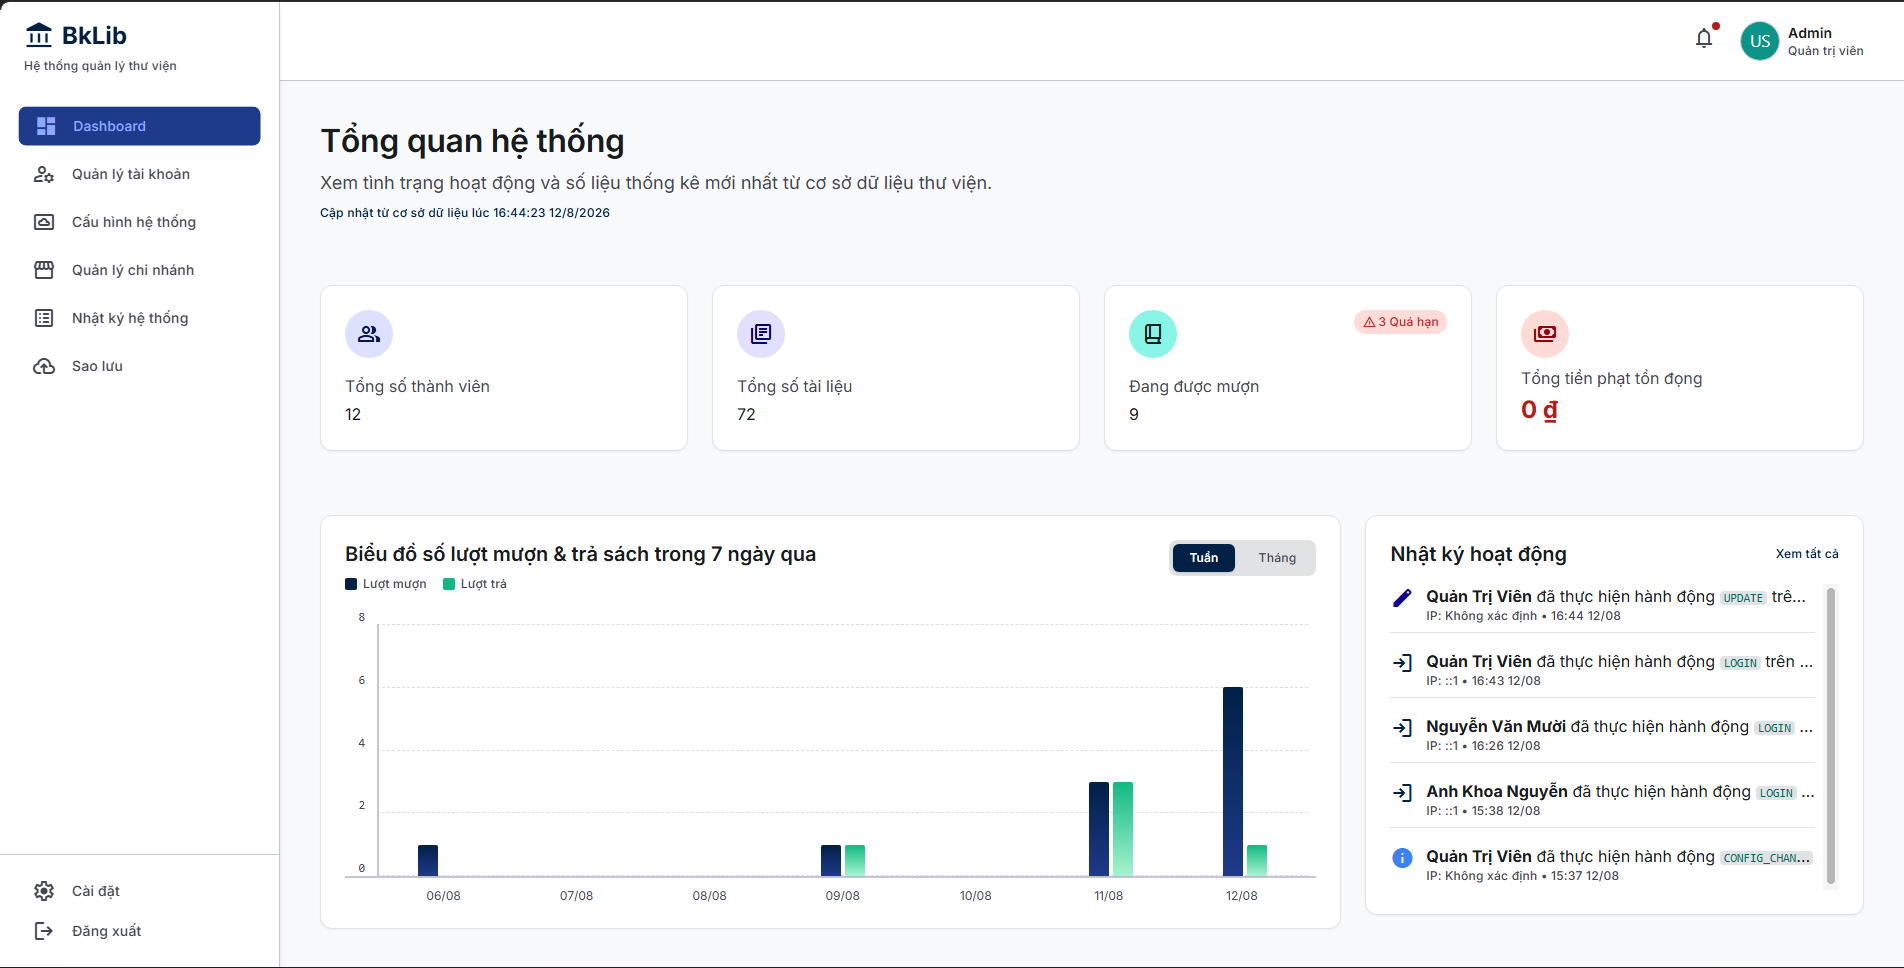
\includegraphics[width=0.95\linewidth]{Images/Admin_Dashboard.png}
    \vspace{10pt}
    \caption{Bảng điều khiển Tổng quan Hệ thống cho Quản trị viên}
    \label{fig:admin_dashboard}
\end{figure}

\textbf{Bố cục \& Chức năng:} Hiển thị các thẻ chỉ số hệ thống (Tổng số tài khoản đang hoạt động, Quy mô danh mục, Số phiên làm việc), chỉ báo lưu trữ cơ sở dữ liệu đám mây, đồ thị lưu lượng API và các cảnh báo an ninh theo thời gian thực.

\paragraph{Trang Quản lý Tài khoản Người dùng}
Không gian làm việc tập trung cho vòng đời tài khoản người dùng, phân quyền và quản lý vai trò.

\begin{figure}[H]
    \centering
    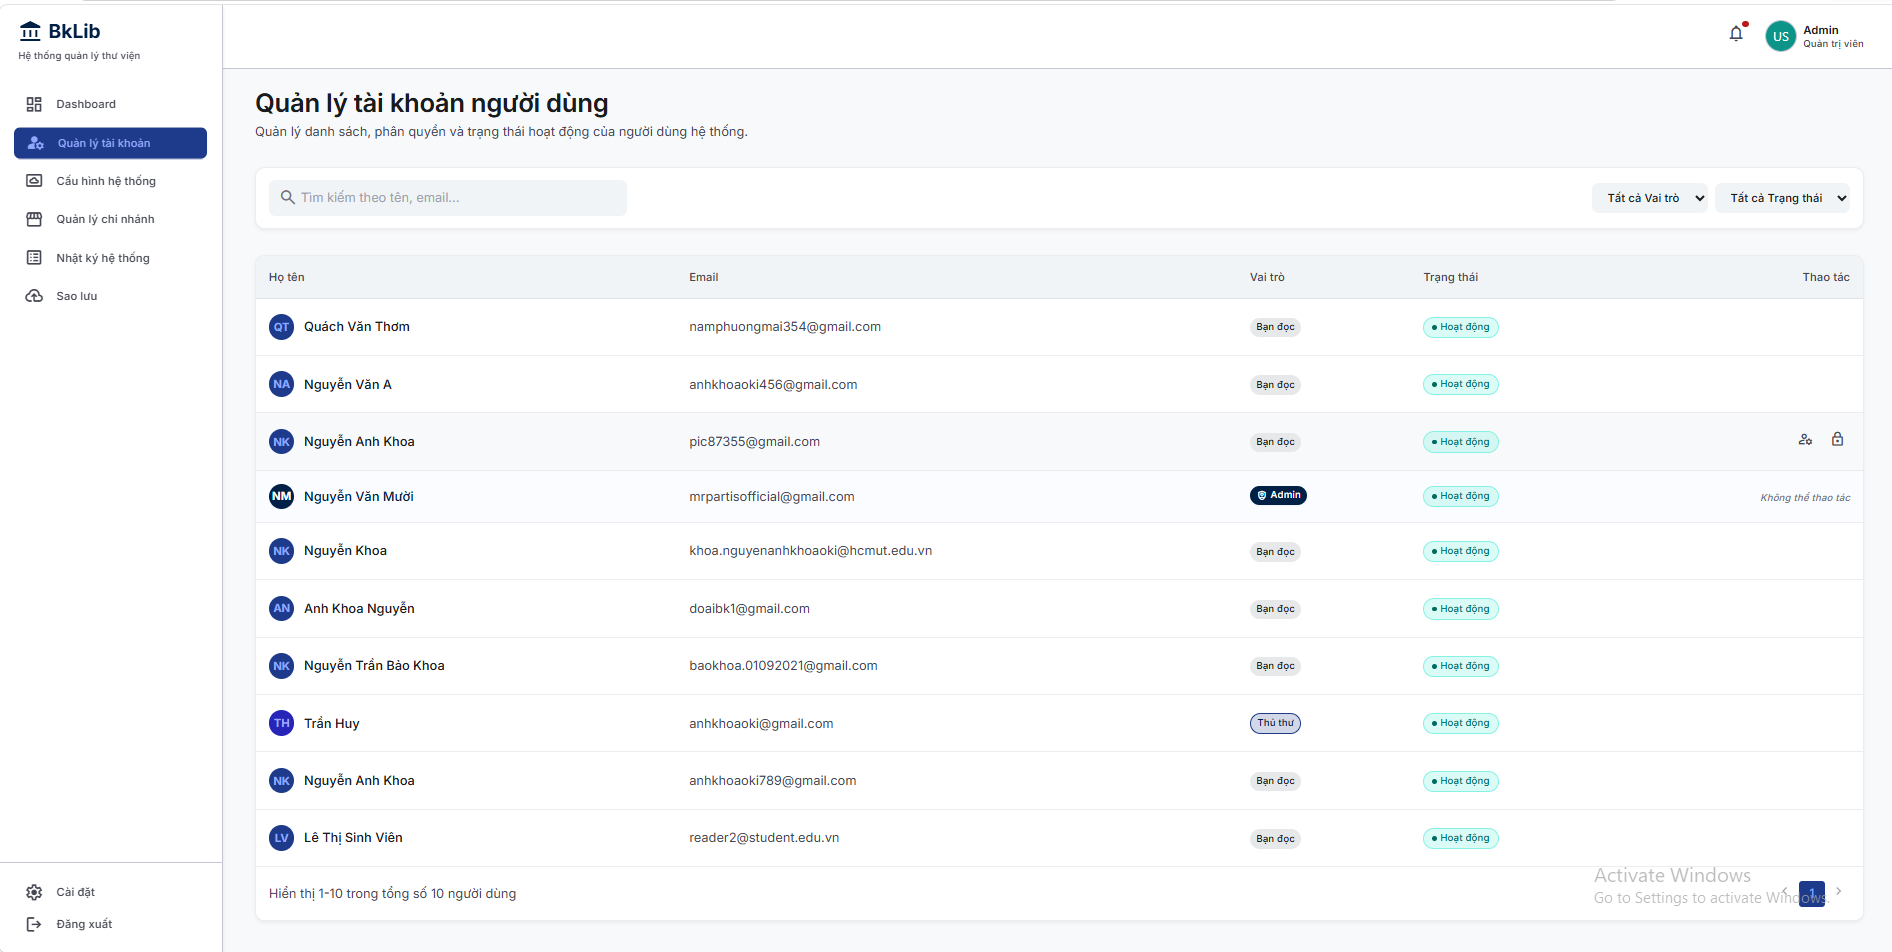
\includegraphics[width=0.95\linewidth]{Images/Admin_QuanLyTaiKhoan.png}
    \vspace{10pt}
    \caption{Giao diện Quản lý Tài khoản Người dùng}
    \label{fig:admin_user_management}
\end{figure}

\textbf{Bố cục \& Chức năng:} Danh mục người dùng phân trang với bộ lọc vai trò (Độc giả, Thủ thư, Admin), nút mở modal tạo tài khoản, công cụ gán quyền RBAC và công tắc khóa/mở khóa tài khoản khẩn cấp.

\paragraph{Trang Cấu hình Hệ thống}
Giao diện quản trị tập trung để định nghĩa các tham số vận hành hệ thống, quy tắc lưu thông và cấu trúc phạt.

\begin{figure}[H]
    \centering
    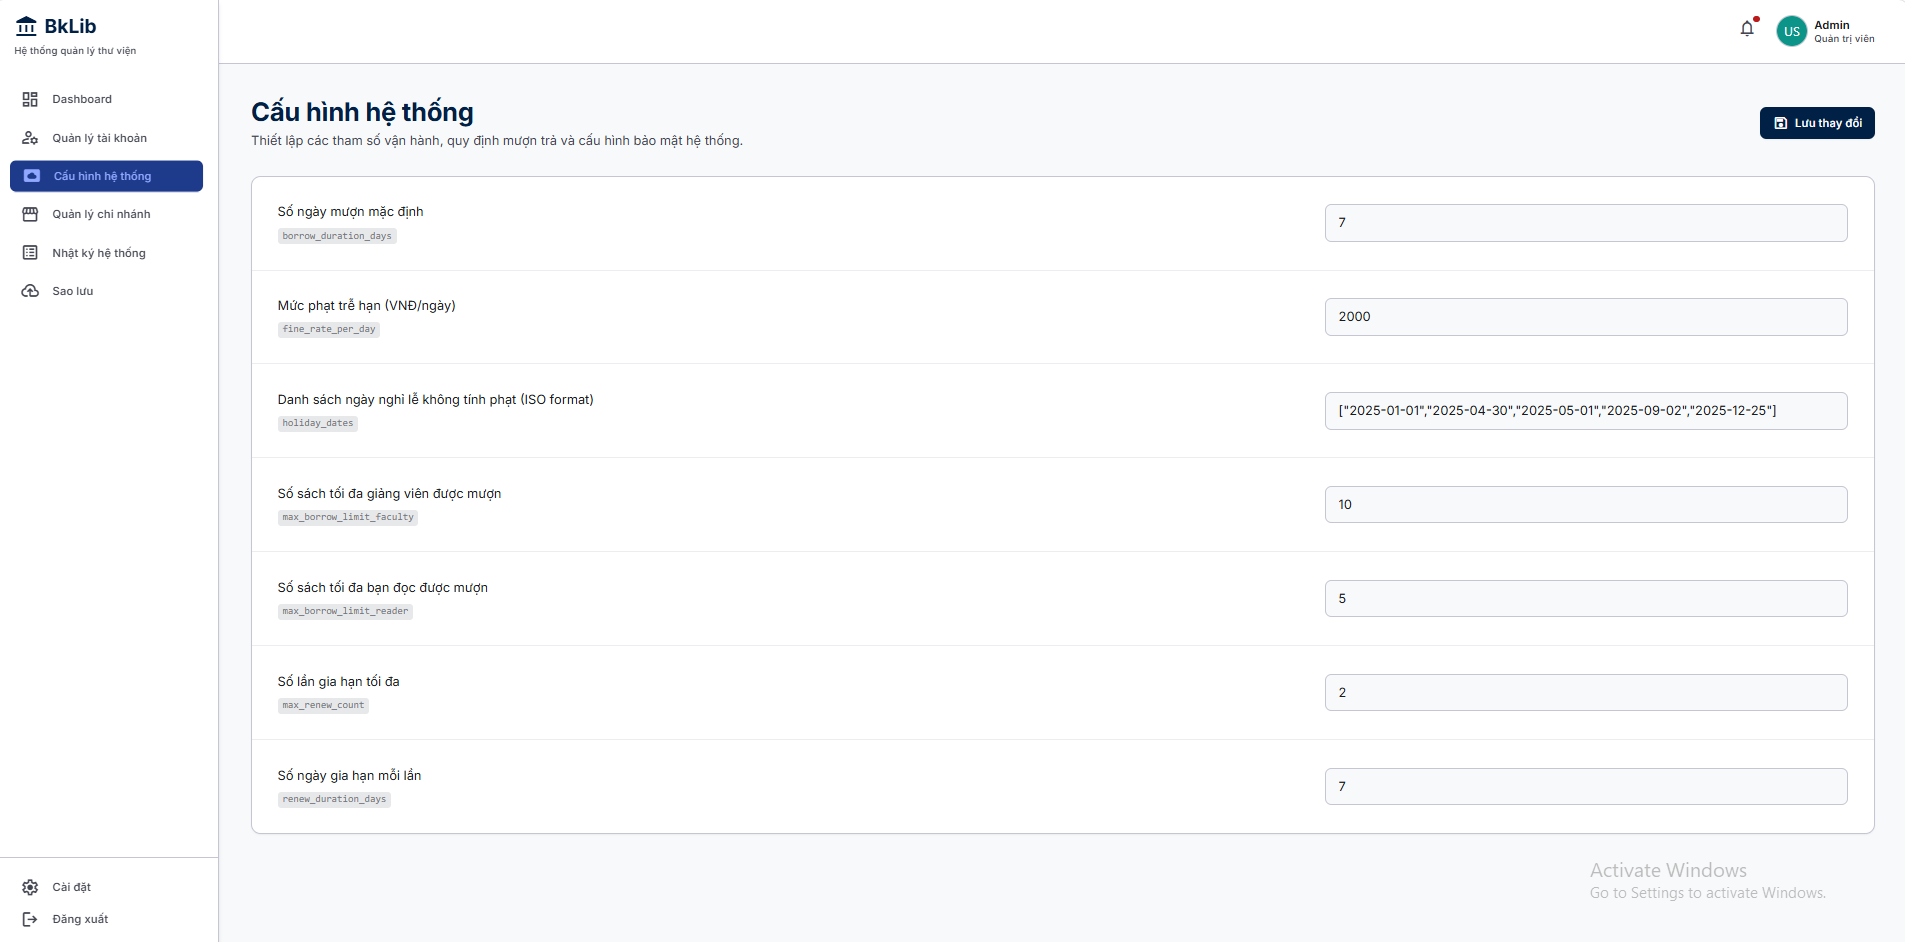
\includegraphics[width=0.95\linewidth]{Images/Admin_CauHinhHeThong.png}
    \vspace{10pt}
    \caption{Giao diện Cấu hình Hệ thống}
    \label{fig:admin_system_config}
\end{figure}

\textbf{Bố cục \& Chức năng:} Bảng cấu hình có cấu trúc cung cấp các ô nhập liệu tương tác cho các biến môi trường hệ thống toàn cục, bao gồm:
\begin{itemize}
    \item \textbf{Quy tắc Lưu thông:} Thời hạn mượn mặc định tính theo ngày (\texttt{borrow\_duration\_days}), hạn mức mượn tối đa cho giảng viên (\texttt{max\_borrow\_limit\_faculty}) và hạn mức mượn chung cho độc giả (\texttt{max\_borrow\_limit\_reader}).
    \item \textbf{Chính sách Gia hạn:} Số lần gia hạn tối đa cho phép (\texttt{max\_renew\_count}) và số ngày kéo dài cho mỗi lần gia hạn (\texttt{renew\_duration\_days}).
    \item \textbf{Cài đặt Tài chính \& Lịch:} Mức phí phạt quá hạn hằng ngày tính theo VNĐ (\texttt{fine\_rate\_per\_day}) và danh sách các ngày nghỉ lễ (\texttt{holiday\_dates}) định dạng ISO để tạm dừng tính phạt trong các ngày nghỉ.
\end{itemize}

\paragraph{Trang Quản lý Chi nhánh}
Trang cấu hình mạng lưới chi nhánh thư viện vật lý và chính sách chuyển sách liên chi nhánh.

\begin{figure}[H]
    \centering
    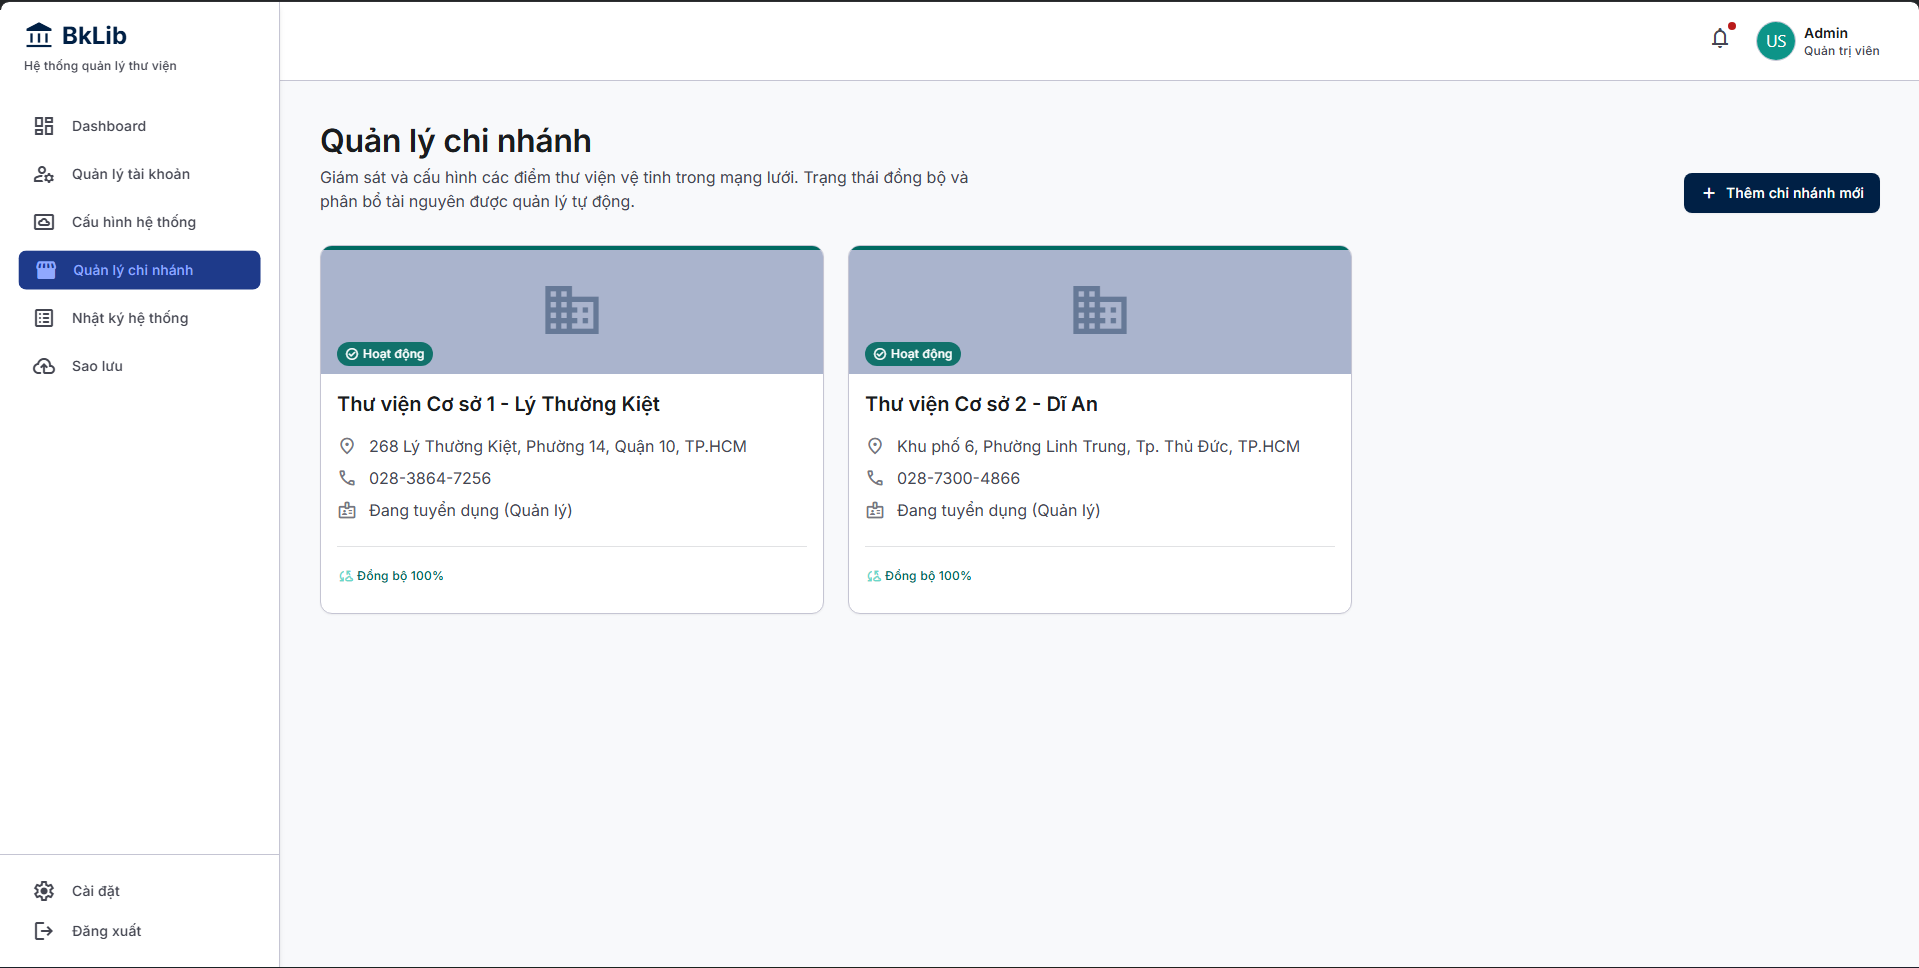
\includegraphics[width=0.95\linewidth]{Images/Admin_QuanLyChiNhanh.png}
    \vspace{10pt}
    \caption{Giao diện Quản lý Chi nhánh}
    \label{fig:admin_branch_management}
\end{figure}

\textbf{Bố cục \& Chức năng:} Lưới các thẻ thông tin chi nhánh hiển thị địa chỉ, chi tiết liên hệ, thủ thư trưởng được phân công, giờ mở cửa và trạng thái đồng bộ với cơ sở dữ liệu trung tâm.

\paragraph{Trang Nhật ký Kiểm toán}
Trình xem nhật ký kiểm toán an ninh ghi lại các hành động quan trọng và các thay đổi trạng thái dữ liệu.

\begin{figure}[H]
    \centering
    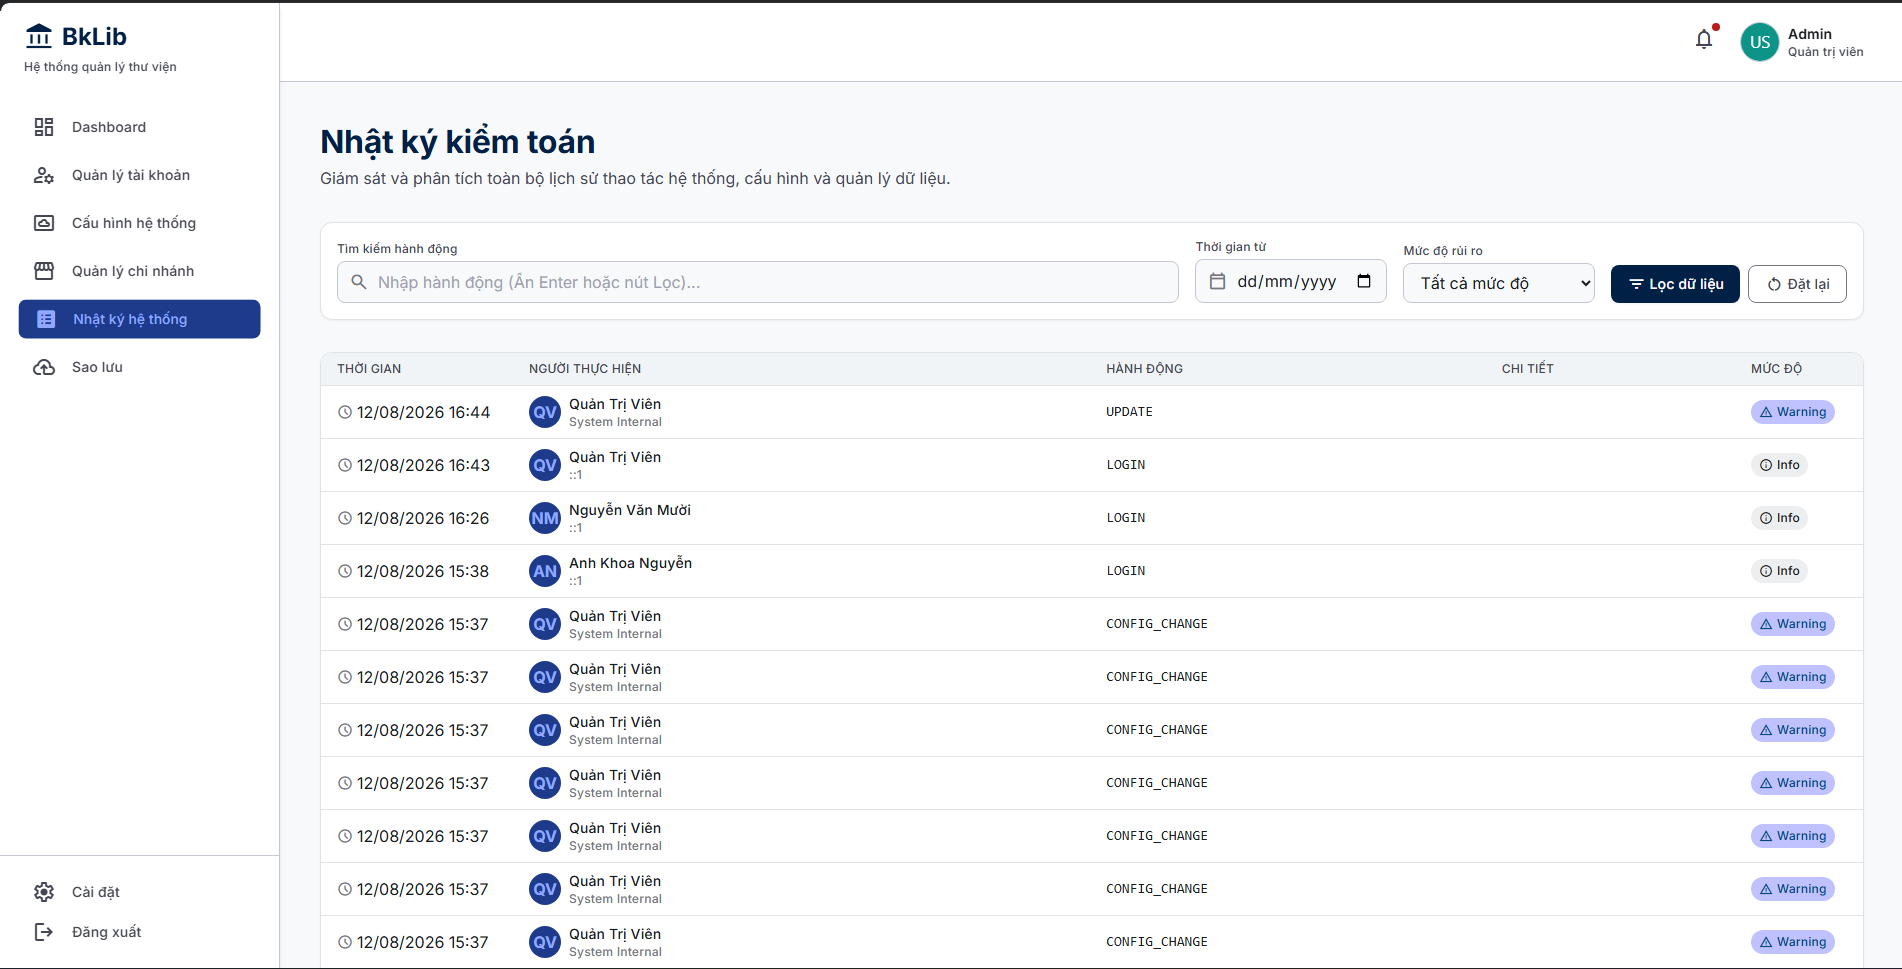
\includegraphics[width=0.95\linewidth]{Images/Admin_NhatKyKiemToan.png}
    \vspace{10pt}
    \caption{Giao diện Nhật ký Kiểm toán Hệ thống}
    \label{fig:admin_audit_log}
\end{figure}

\textbf{Bố cục \& Chức năng:} Bảng sự kiện kiểm toán hiển thị mốc thời gian hành động, danh tính người thực hiện và địa chỉ IP, đường dẫn điểm cuối API, khác biệt dữ liệu JSON trước/sau và huy hiệu mức độ nghiêm trọng để theo dõi bất thường.

\paragraph{Trang Sao lưu \& Phục hồi Dữ liệu}
Công cụ quản lý các bản sao lưu cơ sở dữ liệu và khôi phục sự cố.

\begin{figure}[H]
    \centering
    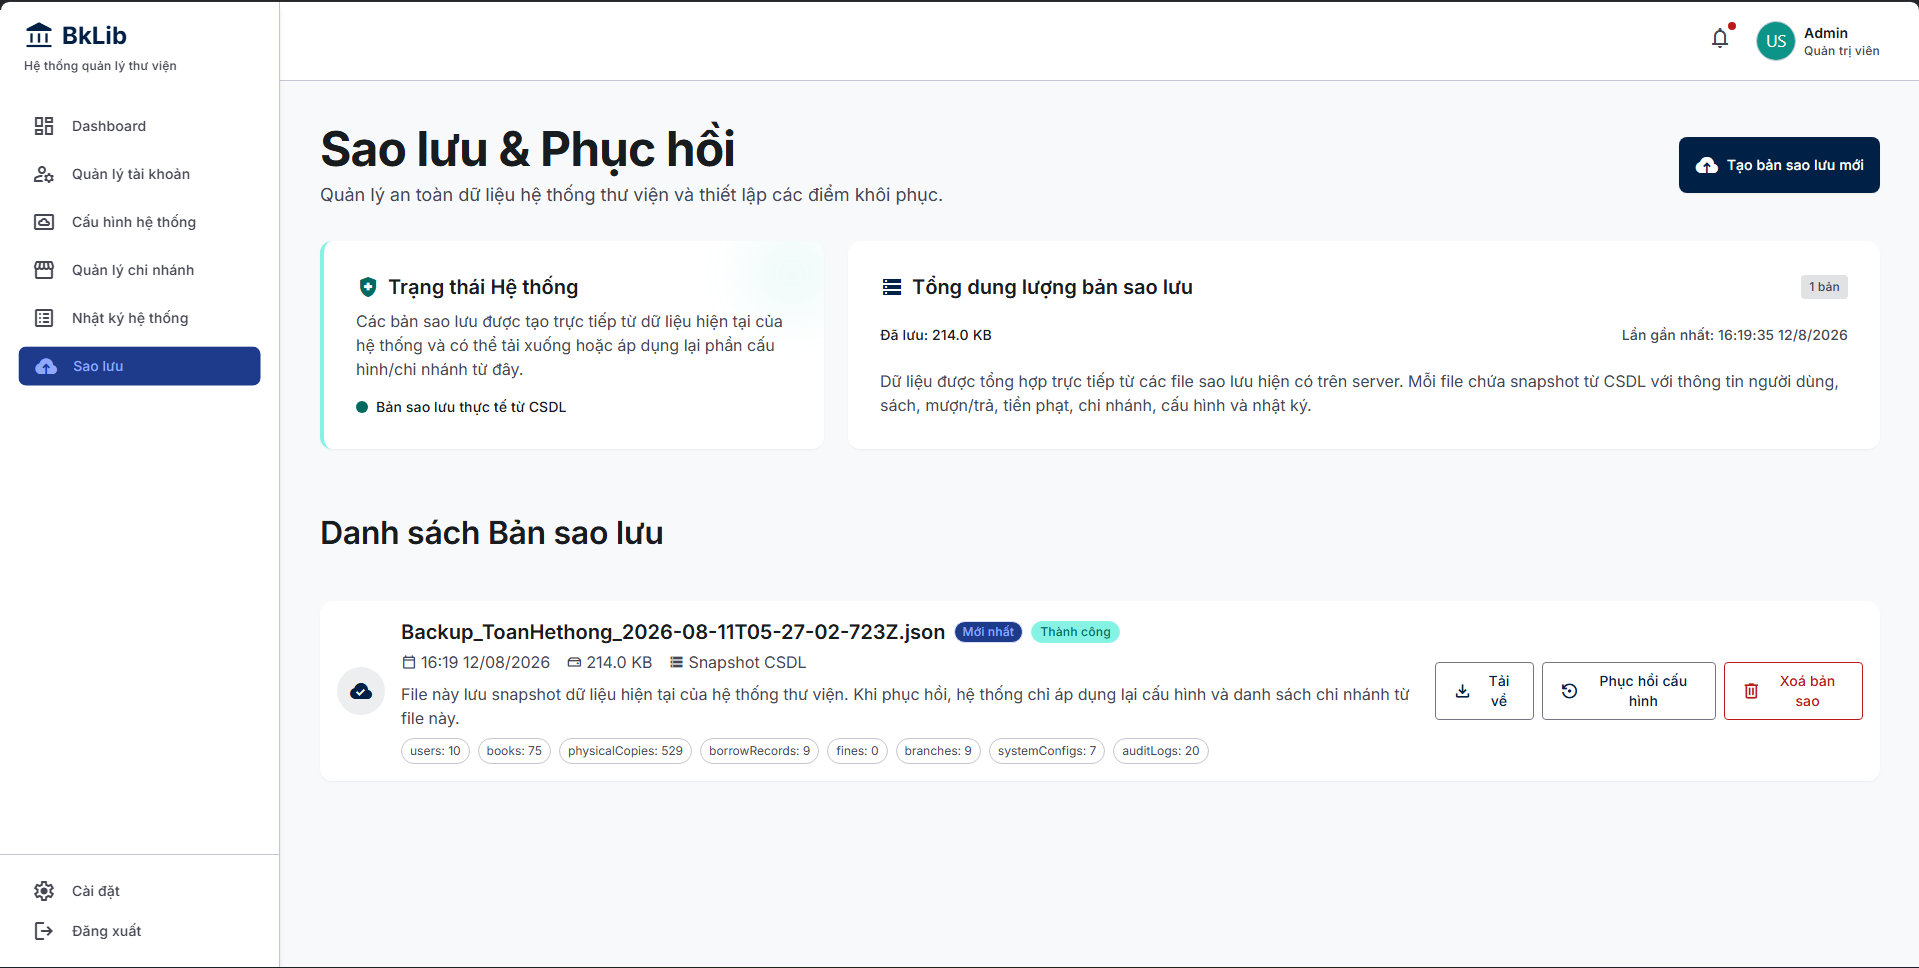
\includegraphics[width=0.95\linewidth]{Images/Admin_SaoLuuPhucHoi.png}
    \vspace{10pt}
    \caption{Giao diện Sao lưu và Phục hồi Dữ liệu}
    \label{fig:admin_backup}
\end{figure}

\textbf{Bố cục \& Chức năng:} Hiển thị cấu hình lịch sao lưu tự động, dung lượng lưu trữ bản sao, nút kích hoạt sao lưu ngay tức thì, nhật ký các bản sao lưu lịch sử và công cụ khôi phục cơ sở dữ liệu về một mốc thời gian cụ thể.

\subsubsection{Các Điểm sáng Hiện thực Kỹ thuật}

Các thao tác quản trị làm thay đổi dữ liệu (như điều chỉnh cấu hình hệ thống, sao lưu cơ sở dữ liệu hay cập nhật tài khoản) tự động ghi lại các bản ghi kiểm toán bất biến chứa dữ liệu người thực hiện và các tham số hành động.

\begin{lstlisting}[caption={Ghi Nhật ký Kiểm toán (backend-express/src/modules/admin/admin.service.ts)}, label={lst:audit_log}]
await prisma.auditLog.create({
  data: {
    actorId: processedById,
    action: AuditAction.SYSTEM_CONFIG_UPDATE,
    targetResource: 'SystemConfig',
    details: { key, oldValue, newValue },
    ipAddress,
  },
});
\end{lstlisting}

% =========================================================================
% SECTION 5.6: DEPLOYMENT STAGE
% =========================================================================
\subsection{Giai đoạn Triển khai}

Phần này mô tả chiến lược triển khai và thiết lập hạ tầng cho hệ thống. Hệ thống được phân phối trên các nhà cung cấp dịch vụ đám mây khác nhau nhằm tận dụng tối đa thế mạnh riêng của từng nền tảng: Vercel được sử dụng cho giao diện frontend và backend Express nhờ khả năng tích hợp CI/CD mượt mà và kiến trúc serverless, trong khi Google Cloud Run được sử dụng cho dịch vụ AI để xử lý hiệu quả các tác vụ máy học được đóng gói dạng container.

\subsubsection{Triển khai Frontend}
Ứng dụng frontend, được xây dựng bằng React và Vite, được triển khai trên Vercel. Vercel cung cấp Mạng lưới Edge Toàn cầu (Edge Network) đảm bảo phân phối nội dung nhanh chóng và tính khả dụng cao. Quy trình triển khai được tích hợp trực tiếp với kho lưu trữ GitHub. Mỗi khi có thao tác push lên nhánh chính (main branch), Vercel sẽ tự động kích hoạt quy trình build mới, thực thi kịch bản biên dịch sản phẩm (production build) và cập nhật trang web trực tuyến. Các biến môi trường, chẳng hạn như URL API backend, được quản lý an toàn trong bảng điều khiển Vercel.

\subsubsection{Triển khai Backend}
Dịch vụ backend, được xây dựng với Node.js và Express, cũng được triển khai trên Vercel bằng cách sử dụng các Hàm Serverless (Serverless Functions). Tiếp cận này loại bỏ nhu cầu tự quản trị máy chủ thủ công và tự động mở rộng quy mô dựa trên lưu lượng truy cập thực tế.
Để cấu hình triển khai, tệp \texttt{vercel.json} được sử dụng tại thư mục gốc của backend để chỉ định môi trường build và các quy tắc định tuyến. Cấu hình điều hướng tất cả các yêu cầu API đến điểm đầu vào chính \texttt{src/app.ts}, sử dụng môi trường thực thi \texttt{@vercel/node}:

\begin{verbatim}
{
  "version": 2,
  "builds": [
    {
      "src": "src/app.ts",
      "use": "@vercel/node"
    }
  ],
  "routes": [
    {
      "src": "/(.*)",
      "dest": "src/app.ts"
    }
  ]
}
\end{verbatim}
Cấu hình này cho phép việc định tuyến của Express hoạt động mượt mà trong môi trường serverless.

\subsubsection{Triển khai Dịch vụ AI}
Dịch vụ AI, chịu trách nhiệm xử lý các tác vụ tiêu tốn tài nguyên như xử lý ngôn ngữ tự nhiên và tìm kiếm ngữ nghĩa, được phát triển bằng Python. Dịch vụ này yêu cầu môi trường thực thi riêng biệt với các phụ thuộc phức tạp được định nghĩa trong \texttt{requirements.txt}. Để đảm bảo tính nhất quán giữa các môi trường, dịch vụ được đóng gói bằng Docker và triển khai lên Google Cloud Run.

\begin{itemize}
    \item \textbf{Đóng gói Container:} Tệp \texttt{Dockerfile} được sử dụng để đóng gói ứng dụng Python, các phụ thuộc hệ thống và các gói thư viện Python thành một hình ảnh Docker (Docker image) tiêu chuẩn.
    \item \textbf{Google Cloud Run:} Cloud Run là một nền tảng tính toán được quản lý hoàn toàn, tự động mở rộng quy mô các container không lưu trạng thái. Nền tảng này được lựa chọn cho dịch vụ AI vì có thể cung cấp hiệu quả các tài nguyên CPU và bộ nhớ cần thiết cho các yêu cầu xử lý và tự động thu hẹp về 0 khi không có truy cập, giúp tối ưu hóa chi phí vận hành.
    \item \textbf{Quy trình Triển khai:} Hình ảnh Docker được biên dịch và đẩy lên Google Artifact Registry. Một dịch vụ Cloud Run sau đó được triển khai tham chiếu đến hình ảnh đã tải lên. Dịch vụ được cấu hình an toàn với các biến môi trường cần thiết và được cấp phát đủ tài nguyên để xử lý các tải công việc AI đồng thời.
\end{itemize}

\subsubsection{Tích hợp Hệ thống}
Kiến trúc triển khai độc lập đảm bảo rằng mỗi dịch vụ có thể mở rộng quy mô một cách riêng biệt dựa trên tải thực tế. Frontend giao tiếp với backend Express trên Vercel thông qua các RESTful API bảo mật chuẩn HTTPS. Backend Express, đến lượt mình, sẽ chuyển tiếp các yêu cầu AI chuyên biệt đến điểm cuối Google Cloud Run, đóng vai trò như một API gateway. Chiến lược triển khai mô-đun này giúp tăng cường khả năng chịu lỗi, tính dễ bảo trì và khả năng mở rộng của toàn bộ hệ thống.

\endgroup
\newpage
\section{Kiểm thử Hệ thống}

\subsection{Mục tiêu và Môi trường Kiểm thử}

Quá trình kiểm thử được thực hiện nhằm đánh giá tính đúng đắn của các chức năng quản lý thư viện, sự phối hợp giữa các tầng hệ thống, các quy trình nghiệp vụ chính và các yêu cầu về an ninh, xử lý lỗi. Phạm vi tập trung vào backend Express/TypeScript, bao gồm các mô-đun về xác thực, người dùng, sách, chi nhánh, lưu thông tài liệu và các tính năng AI.\\

\textbf{Các Công cụ Sử dụng}
\begin{itemize}
        \item Jest kết hợp với ts-jest để thực thi các ca kiểm thử TypeScript.
        \item Supertest để gửi các yêu cầu HTTP đến ứng dụng Express trong quá trình kiểm thử tích hợp và kiểm thử hệ thống.
        \item Mock Prisma Client và các dịch vụ bên ngoài giả lập cho kiểm thử cô lập, loại bỏ sự phụ thuộc vào cơ sở dữ liệu thực hoặc dịch vụ email.
        \item Trình biên dịch TypeScript với cờ \texttt{--noEmit} cùng với Jest để kiểm tra chất lượng mã nguồn.
\end{itemize}

\noindent Mã nguồn kiểm thử được tổ chức trong thư mục \texttt{backend-express/tests}, chia thành bốn danh mục: \texttt{unit}, \texttt{integration}, \texttt{system}, và \texttt{quality}. Các bài kiểm thử chạy trong môi trường Node.js và được cấu hình tập trung trong tệp \texttt{jest.config.js}.

\subsection{Kiểm thử Đơn vị (Unit Testing)}

\textbf{Mục tiêu} \\

Xác minh tính đúng đắn của từng hàm hoặc mô-đun riêng lẻ trong sự cô lập. Các ca kiểm thử tập trung vào logic nghiệp vụ, kiểm tra dữ liệu đầu vào, mã lỗi HTTP, xác thực token, xử lý mật khẩu và các nhánh ngoại lệ. Prisma Client, mailer và các phụ thuộc bên ngoài được thay thế bằng các đối tượng giả lập (mock) để kết quả không bị ảnh hưởng bởi môi trường thực thi.\\

\noindent \textbf{Phương pháp luận} \\

Mỗi hàm được kiểm thử với các trường hợp hợp lệ, không hợp lệ, biên và ngoại lệ. Các nhóm chức năng chính bao gồm đăng ký và đăng nhập, xác thực OTP, quản lý sách, quản lý độc giả, lưu thông tài liệu, middleware xác thực và chuẩn hóa lỗi.

\begin{table}[H]
\centering
\caption{Phạm vi và Kết quả Kiểm thử Đơn vị}
\begin{tabularx}{\textwidth}{|p{4.2cm}|X|c|c|}
\hline
\textbf{Nhóm Kiểm thử} & \textbf{Nội dung Chính} & \textbf{Suites} & \textbf{Kết quả} \\
\hline
Auth và DTO & Đăng ký, OTP, đăng nhập, kiểm tra dữ liệu đầu vào & 3 & Đạt (Pass) \\
\hline
Sách & CRUD sách, tiện ích sách, quản lý danh mục & 3 & Đạt (Pass) \\
\hline
Người dùng và Chi nhánh & Hồ sơ độc giả, logic nghiệp vụ chi nhánh & 2 & Đạt (Pass) \\
\hline
Lưu thông và Middleware & Mượn/trả, middleware xác thực, xử lý lỗi & 3 & Đạt (Pass) \\
\hline
\multicolumn{2}{|r|}{\textbf{Tổng cộng}} & \textbf{10} & \textbf{168/168} \\
\hline
\end{tabularx}
\end{table}

Ví dụ dưới đây kiểm thử kịch bản đăng ký với một email đã tồn tại. Kết quả kỳ vọng là dịch vụ trả về lỗi HTTP 409 và không tạo tài khoản mới.

\begin{lstlisting}[language=R, caption={Ca kiểm thử đơn vị cho tính năng đăng ký}]
it('returns 409 when email already exists', async () => {
    prismaMock.user.findUnique.mockResolvedValueOnce({ id: 'exists' });

    await expect(authService.register({
        email: 'reader@example.com',
        password: 'password1',
        fullName: 'A',
    })).rejects.toMatchObject({ statusCode: 409 });
});
\end{lstlisting}

Kết quả kiểm thử đơn vị cho thấy 10/10 bộ kiểm thử (test suites) đã vượt qua, tương ứng với 168/168 ca kiểm thử đạt. Độ bao phủ mã nguồn (code coverage) cho nhóm này đạt 94.33\% câu lệnh (statements), 77.58\% nhánh (branches), 94.44\% hàm (functions) và 95.07\% dòng (lines). \\

\begin{figure}[H]
    \centering
    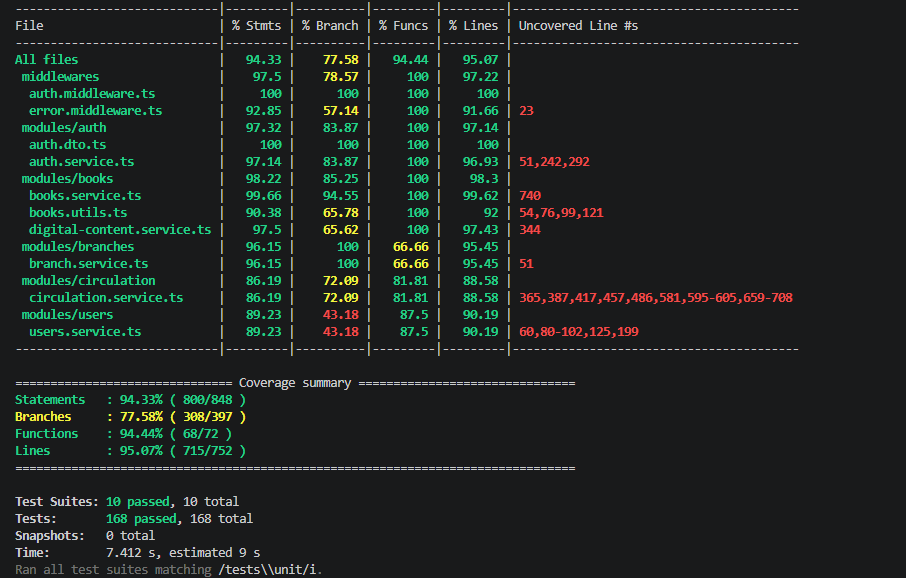
\includegraphics[width=0.9\textwidth]{Images/unit_test_result.png}
    \vspace{0.5cm}
    \caption{Kết quả kiểm thử đơn vị}
    \label{fig:unit-test-result}
\end{figure}

\subsection{Kiểm thử Tích hợp (Integration Testing)}

\textbf{Mục tiêu} \\

Xác minh sự phối hợp giữa các route, middleware, controller, service và tầng truy cập dữ liệu thông qua các yêu cầu HTTP thực tế gửi đến ứng dụng Express. Bộ kiểm thử này xác nhận cấu trúc phản hồi, mã trạng thái HTTP, cơ chế xác thực và sự tích hợp liên chức năng trong cùng mô-đun.\\

\noindent \textbf{Phương pháp luận} \\

Supertest được sử dụng để giả lập các yêu cầu GET, POST, PATCH và DELETE. Prisma Client được giả lập tại ranh giới dữ liệu, trong khi ứng dụng Express được khởi tạo đầy đủ để các route và middleware thực thi giống như trong môi trường thực.

\begin{table}[H]
\centering
\caption{Phạm vi và Kết quả Kiểm thử Tích hợp}
\begin{tabularx}{\textwidth}{|p{4.2cm}|X|c|c|}
\hline
\textbf{API/Mô-đun} & \textbf{Nội dung Kiểm thử} & \textbf{Suites} & \textbf{Kết quả} \\
\hline
Auth & Đăng ký, xác thực OTP, đăng nhập, lỗi dữ liệu đầu vào & 1 & Đạt (Pass) \\
\hline
Sách và Chi nhánh & Tra cứu sách, quản lý danh mục và chi nhánh & 2 & Đạt (Pass) \\
\hline
Người dùng và Lưu thông & Hồ sơ người dùng, mượn, trả, gia hạn & 2 & Đạt (Pass) \\
\hline
Dịch vụ AI & Tương tác với các điểm cuối dịch vụ AI & 1 & Đạt (Pass) \\
\hline
\multicolumn{2}{|r|}{\textbf{Tổng cộng}} & \textbf{6} & \textbf{67/67} \\
\hline
\end{tabularx}
\end{table}

Ví dụ dưới đây kiểm thử API đăng nhập với thông tin hợp lệ. Ngoài mã trạng thái HTTP 200, bài kiểm thử xác nhận nội dung phản hồi chứa access token, refresh token và chi tiết hồ sơ người dùng.

\begin{lstlisting}[language=R, caption={Ca kiểm thử tích hợp cho API đăng nhập}]
const response = await request(app)
    .post('/api/v1/auth/login')
    .send({ email: 'reader@library.edu.vn', password: 'CorrectPass@123' });

expect(response.status).toBe(200);
expect(response.body.success).toBe(true);
expect(response.body.data.accessToken).toBeDefined();
expect(response.body.data.refreshToken).toBeDefined();
\end{lstlisting}

Kiểm thử tích hợp đạt 6/6 bộ kiểm thử và 67/67 ca kiểm thử vượt qua. Tất cả các điểm cuối được đánh giá đều trả về mã trạng thái và nội dung phản hồi phù hợp cho cả kịch bản thành công lẫn kịch bản lỗi. \\

\begin{figure}[H]
    \centering
    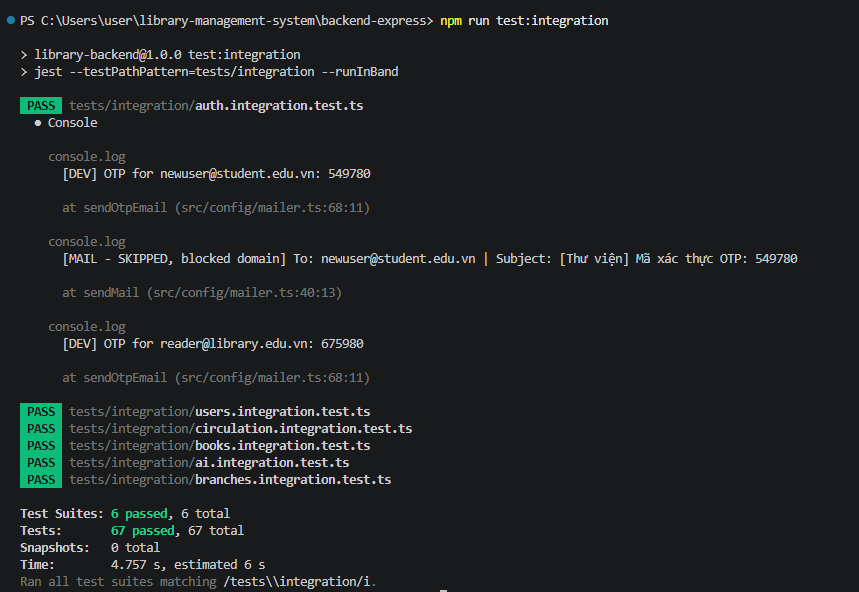
\includegraphics[width=0.9\textwidth]{Images/integration_test_result.png}
    \vspace{0.5cm}
    \caption{Kết quả kiểm thử tích hợp}
    \label{fig:integration-test-result}
\end{figure}


\subsection{Kiểm thử Hệ thống (System Testing)}

\textbf{Mục tiêu} \\ 

Xác nhận các quy trình nghiệp vụ end-to-end từ yêu cầu người dùng đến kết quả đầu ra cuối cùng của hệ thống. Nhóm này tập trung vào vòng đời độc giả, chu trình mượn--gia hạn--trả, hàng chờ đặt chỗ, tính tiền phạt quá hạn và an ninh phân quyền.\\

\noindent \textbf{Phương pháp luận}\\

Các bước nghiệp vụ được giả lập theo thứ tự tuần tự trong thực tế. Mỗi bước gửi một yêu cầu sử dụng vai trò người dùng phù hợp và xác minh cả phản hồi trả về lẫn trạng thái nghiệp vụ được cập nhật. Nhóm kiểm thử an ninh bao gồm các trường hợp biên như thiếu token, token hết hạn, token bị giả mạo, truy cập vai trò không hợp lệ, các header an ninh và điểm cuối không tồn tại.

\begin{table}[H]
\centering
\caption{Các Quy trình Kiểm thử Hệ thống}
\begin{tabularx}{\textwidth}{|p{5cm}|X|c|}
\hline
\textbf{Quy trình Nghiệp vụ} & \textbf{Nội dung Kiểm thử} & \textbf{Kết quả} \\
\hline
Vòng đời Độc giả & Đăng ký, xác thực, cập nhật hồ sơ, sử dụng tài khoản & Đạt (Pass) \\
\hline
Lưu thông Tài liệu & Thêm sách, tìm kiếm, mượn, xem lịch sử, gia hạn, trả & Đạt (Pass) \\
\hline
Đặt chỗ và Hàng chờ & Đặt chỗ tài liệu, thứ tự hàng chờ, thông báo sách về & Đạt (Pass) \\
\hline
Phạt Quá hạn & Phát hiện quá hạn, tạo khoản phạt, xử lý thanh toán & Đạt (Pass) \\
\hline
An ninh Hệ thống & JWT, RBAC, Helmet, lỗi 404, dữ liệu JSON không hợp lệ & Đạt (Pass) \\
\hline
\multicolumn{1}{|r|}{\textbf{Tổng cộng}} & \textbf{5 bộ kiểm thử, 36 ca kiểm thử} & \textbf{36/36} \\
\hline
\end{tabularx}
\end{table}

Ví dụ, quy trình lưu thông lần lượt kiểm tra việc thủ thư thêm sách, độc giả tìm kiếm sách, thủ thư tạo phiếu mượn và độc giả yêu cầu gia hạn. Ca kiểm thử dưới đây xác minh vai trò thủ thư được cấp quyền tạo phiếu mượn:

\begin{lstlisting}[language=R, caption={Ca kiểm thử hệ thống cho quy trình mượn sách}]
const response = await request(app)
    .post('/api/v1/circulation/borrow')
    .set(roleAuthHeader(Role.LIBRARIAN, librarianId))
    .send({ userId: readerId, barcode: copyBarcode });

expect(response.status).toBe(201);
expect(response.body.success).toBe(true);
expect(response.body.data.borrowRecordId).toBe(borrowRecordId);
\end{lstlisting}

Kết quả cho thấy toàn bộ 5 quy trình hệ thống đã vượt qua, với 36/36 ca kiểm thử thành công. Các trường hợp thiếu token, token không hợp lệ, truy cập trái phép và dữ liệu JSON sai định dạng đều bị từ chối chính xác với các mã trạng thái HTTP phù hợp. \\

\begin{figure}[H]
    \centering
    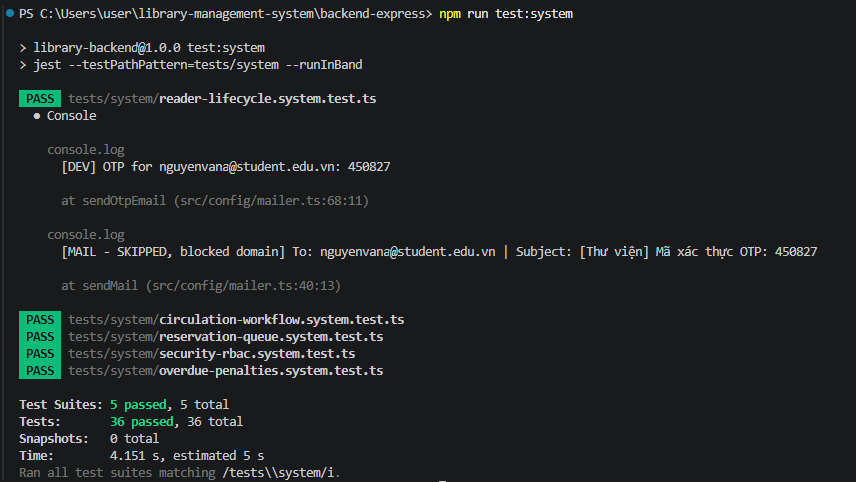
\includegraphics[width=0.9\textwidth]{Images/system_test_result.png}
    \vspace{0.5cm}
    \caption{Kết quả kiểm thử hệ thống}
    \label{fig:system-test-result}
\end{figure}

\subsection{Kiểm thử Chất lượng Mã nguồn (Code Quality Testing)}

\textbf{Mục tiêu} \\

Đánh giá các điều kiện chất lượng tĩnh và quy ước kiến trúc bên cạnh việc kiểm thử chức năng. Các chủ đề xác minh bao gồm biên dịch TypeScript, tính toàn vẹn thư mục nguồn, phát hiện secret hardcode, phân tầng route--service, cấu trúc phản hồi API và mã lỗi chuẩn hóa.\\

\noindent \textbf{Phương pháp luận} \\ 

Các bài kiểm thử phân tích các tệp TypeScript trong thư mục \texttt{src} đồng thời thực thi \texttt{npx tsc --noEmit}. Các tiêu chí được diễn đạt dưới dạng các khẳng định Jest để bất kỳ vi phạm nào cũng tự động bị bắt trong đường ống kiểm thử.

\begin{table}[H]
\centering
\caption{Kết quả Kiểm thử Chất lượng Mã nguồn}
\begin{tabularx}{\textwidth}{|p{6cm}|X|c|}
\hline
\textbf{Tiêu chí} & \textbf{Nội dung Kiểm thử} & \textbf{Kết quả} \\
\hline
Biên dịch TypeScript & Toàn bộ backend biên dịch không có lỗi kiểu & Đạt (Pass) \\
\hline
Tính Toàn vẹn Mã nguồn & Thư mục \texttt{src} tồn tại; các tệp TypeScript không rỗng & Đạt (Pass) \\
\hline
An ninh & Không có mật khẩu, secret JWT hay chuỗi kết nối hardcode & Đạt (Pass) \\
\hline
Kiến trúc Phân tầng & Route không gọi Prisma trực tiếp; controller chuyển lỗi qua \texttt{next} & Đạt (Pass) \\
\hline
Phản hồi và Mã Lỗi & Thuộc tính \texttt{success} chuẩn hóa và mã trạng thái HTTP hợp lệ & Đạt (Pass) \\
\hline
\multicolumn{1}{|r|}{\textbf{Tổng cộng}} & \textbf{2 bộ kiểm thử, 10 ca kiểm thử} & \textbf{10/10} \\
\hline
\end{tabularx}
\end{table}

\begin{figure}[H]
    \centering
    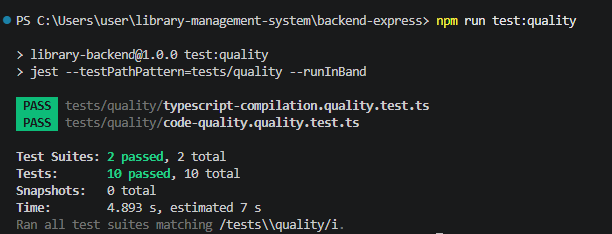
\includegraphics[width=0.9\textwidth]{Images/quality_test_result.png}
    \vspace{0.5cm}
    \caption{Kết quả kiểm thử chất lượng mã nguồn}
    \label{fig:quality-test-result}
\end{figure}

\subsection{Tổng kết Kiểm thử}

Tất cả các bài kiểm thử backend đã được thực thi bằng lệnh \texttt{npm test -- --runInBand}. Tổng hợp chung được trình bày trong Bảng~\ref{tab:test-summary}.

\begin{table}[H]
\centering
\caption{Tổng kết Kiểm thử Backend}
\label{tab:test-summary}
\begin{tabular}{|l|r|r|r|}
\hline
\textbf{Loại Kiểm thử} & \textbf{Bộ Kiểm thử (Suites)} & \textbf{Ca Kiểm thử (Cases)} & \textbf{Đạt (Passed)} \\
\hline
Kiểm thử Đơn vị (Unit) & 10 & 168 & 168 \\
\hline
Kiểm thử Tích hợp (Integration) & 6 & 67 & 67 \\
\hline
Kiểm thử Hệ thống (System) & 5 & 36 & 36 \\
\hline
Chất lượng Mã nguồn (Quality) & 2 & 10 & 10 \\
\hline
\textbf{Tổng cộng} & \textbf{23} & \textbf{281} & \textbf{281} \\
\hline
\end{tabular}
\end{table}

\noindent Toàn bộ 23 bộ kiểm thử đã thực thi thành công với 0 ca kiểm thử thất bại và không có bài kiểm thử snapshot. Các kết quả này xác nhận rằng các chức năng chính, sự phối hợp liên tầng, các quy tắc an ninh và tiêu chuẩn chất lượng mã nguồn của backend đều đáp ứng đầy đủ các yêu cầu kiểm thử tại thời điểm đánh giá. \\

\begin{figure}[H]
    \centering
    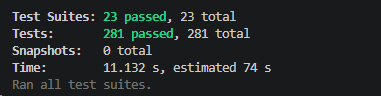
\includegraphics[width=0.9\textwidth]{Images/summary_test_result.png}
    \vspace{0.5cm}
    \caption{Tổng kết kết quả kiểm thử}
    \label{fig:summary-test-result}
\end{figure}
\newpage
\section{Đánh giá các Tính năng AI}

\subsection{Tại sao Kiểm thử Truyền thống Không Đủ cho AI}

Phương pháp luận kiểm thử được mô tả trong chương trước tuân theo mô hình \textbf{định tính (deterministic)}: với bất kỳ đầu vào cho trước nào, hệ thống phải tạo ra đầu ra được xác định chính xác, và một phép kiểm tra (assertion) chỉ có thể đạt (pass) hoặc thất bại (fail). Mô hình này hoạt động tốt cho các hàm không lưu trạng thái (stateless) và các điểm cuối REST API nơi hành vi mang tính dự đoán được và có giới hạn.

Tuy nhiên, các tính năng tích hợp AI trong BkLib — cụ thể là Chatbot dựa trên RAG và Động cơ Tìm kiếm Ngữ nghĩa — tạo ra các đầu ra \textbf{không định tính (non-deterministic)} dưới dạng ngôn ngữ tự nhiên. Hãy xem xét sự đối lập sau:

\begin{table}[H]
\centering
\caption{Kiểm thử Định tính vs. Đánh giá Tính năng AI}
\begin{tabularx}{\textwidth}{|p{3.5cm}|X|X|}
\hline
\textbf{Khía cạnh} & \textbf{Kiểm thử Truyền thống} & \textbf{Đánh giá Tính năng AI} \\
\hline
Kiểu đầu ra & Giá trị cố định (mã trạng thái, trường JSON) & Câu ngôn ngữ tự nhiên hoặc danh sách xếp hạng \\
\hline
Kiểm tra tính đúng đắn & \texttt{expect(x).toBe(y)} & Độ tương đồng ngữ nghĩa, độ trung thực, độ liên quan \\
\hline
Mức độ biến đổi & Không có — đầu vào giống nhau cho đầu ra giống nhau & Cao — diễn đạt thay đổi qua từng lần chạy \\
\hline
Công cụ & Jest, Supertest & LLM-as-a-Judge, độ tương đồng cosine vector \\
\hline
\end{tabularx}
\end{table}

\noindent Ví dụ, khi độc giả hỏi \textit{``Tôi có thể mượn tối đa bao nhiêu quyển sách cùng lúc?''}, phản hồi hợp lệ của chatbot có thể là \textit{``Bạn có thể mượn tối đa 5 quyển sách cho mỗi lần mượn''} hoặc \textit{``Thư viện quy định hạn mức tối đa 5 tài liệu cho mỗi độc giả''} — cả hai đều đúng về mặt ngữ nghĩa nhưng khác nhau về mặt từ ngữ. Phép kiểm tra cứng \texttt{toBe()} không thể nắm bắt được sự tương đương này, do đó cần phải có một khung đánh giá AI chuyên biệt.

\subsection{Phương pháp luận AI-as-a-Judge}

Đồ án áp dụng phương pháp luận \textbf{LLM-as-a-Judge} (sử dụng một LLM mạnh hơn để đánh giá đầu ra của hệ thống) kết hợp với truy vấn vector trực tiếp để đánh giá định lượng cả hai dịch vụ AI.

%\begin{figure}[H]
%\centering
%\includegraphics[width=0.85\textwidth]{Images/ai_eval_architecture.png}
%\caption{Kiến trúc Đánh giá AI}
%\label{fig:ai_eval_arch}
%\end{figure}

\subsubsection{Các Chỉ số Đánh giá Chatbot (Khung RAG)}

Mô-đun Chatbot sử dụng RAG được đánh giá trên ba chỉ số cốt lõi, mỗi chỉ số được chấm trên thang điểm 1--5 bởi một mô hình giám khảo độc lập:

\begin{enumerate}
    \item \textbf{Độ trung thực (Faithfulness) [1--5]:} Đo lường xem câu trả lời của Chatbot có hoàn toàn dựa trên các đoạn văn bản ngữ cảnh được truy xuất hay không, hay chứa thông tin suy diễn không có thực (hallucination).
    \item \textbf{Độ liên quan (Answer Relevancy) [1--5]:} Đo lường mức độ câu trả lời giải quyết trực tiếp câu hỏi của người dùng mà không lan man hoặc trả lời lạc đề.
    \item \textbf{Độ chính xác (Correctness) [1--5]:} So sánh câu trả lời được tạo với câu trả lời chuẩn (Ground Truth) được gắn nhãn bởi con người về mặt ngữ nghĩa.
\end{enumerate}

\subsubsection{Các Chỉ số Đánh giá Tìm kiếm Ngữ nghĩa}

Tính năng Tìm kiếm Ngữ nghĩa được đánh giá dựa trên tiêu chuẩn truy xuất thông tin:

\begin{enumerate}
    \item \textbf{Top-K Accuracy (Hit@K):} Tỷ lệ phần trăm các câu truy vấn mà ít nhất một tài liệu liên quan xuất hiện trong $K$ kết quả đầu tiên (với $K=3$ và $K=5$).
    \item \textbf{Mean Reciprocal Rank (MRR):} Điểm trung bình của vị trí nghịch đảo cho tài liệu liên quan đầu tiên tìm thấy:
    \begin{equation}
    \text{MRR} = \frac{1}{|Q|} \sum_{i=1}^{|Q|} \frac{1}{\text{rank}_i}
    \end{equation}
\end{enumerate}

\subsection{Kết quả Đánh giá Chatbot (RAG)}

\subsubsection{Thiết lập Bộ dữ liệu Kiểm thử}

Bộ dữ liệu kiểm thử Chatbot bao gồm **16 ca kiểm thử** đại diện cho 4 nhóm nghiệp vụ chính:
\begin{itemize}
    \item \textbf{Quy định mượn trả (Borrowing Rules):} 5 ca kiểm thử (CB-01 đến CB-05).
    \item \textbf{Thủ tục gia hạn và đặt chỗ (Renewal \& Holds):} 4 ca kiểm thử (CB-06 đến CB-09).
    \item \textbf{Phí phạt quá hạn và chính sách (Fines \& Policy):} 4 ca kiểm thử (CB-10 đến CB-13).
    \item \textbf{Truy vấn ngoài phạm vi / Khóa tài khoản (Out-of-Scope / Account Lock):} 3 ca kiểm thử (CB-14 đến CB-16).
\end{itemize}

\subsubsection{Bảng Kết quả Đánh giá Chatbot Chi tiết}

Bảng~\ref{tab:chatbot_eval_results} trình bày chi tiết kết quả đánh giá cho toàn bộ 16 ca kiểm thử.

\begin{table}[H]
\centering
\caption{Kết quả Đánh giá Chi tiết Chatbot RAG (Thang điểm 1--5)}
\label{tab:chatbot_eval_results}
\begin{tabularx}{\textwidth}{|l|p{3.2cm}|X|c|c|c|}
\hline
\textbf{ID} & \textbf{Nhóm Nghiệp vụ} & \textbf{Nội dung Câu hỏi} & \textbf{Faith.} & \textbf{Relev.} & \textbf{Correct.} \\
\hline
CB-01 & Mượn trả & Mượn tối đa bao nhiêu quyển sách? & 5 & 5 & 5 \\
\hline
CB-02 & Mượn trả & Sinh viên được mượn sách trong bao lâu? & 5 & 5 & 5 \\
\hline
CB-03 & Mượn trả & Giảng viên có hạn mức mượn khác không? & 5 & 5 & 5 \\
\hline
CB-04 & Mượn trả & Tôi có thể mượn tạp chí in không? & 5 & 5 & 5 \\
\hline
CB-05 & Mượn trả & Quy trình mượn sách trực tiếp tại quầy? & 5 & 4 & 5 \\
\hline
CB-06 & Gia hạn \& Đặt chỗ & Cách gia hạn sách trực tuyến? & 5 & 5 & 5 \\
\hline
CB-07 & Gia hạn \& Đặt chỗ & Sách có người đặt chỗ có gia hạn được không? & 5 & 5 & 5 \\
\hline
CB-08 & Gia hạn \& Đặt chỗ & Được gia hạn tối đa bao nhiêu lần? & 5 & 5 & 5 \\
\hline
CB-09 & Gia hạn \& Đặt chỗ & Làm sao biết sách đặt chỗ đã về? & 5 & 5 & 5 \\
\hline
CB-10 & Phí phạt & Mức phạt trả sách quá hạn 1 ngày? & 5 & 5 & 5 \\
\hline
CB-11 & Phí phạt & Ngày nghỉ lễ có tính phí phạt không? & 5 & 5 & 5 \\
\hline
CB-12 & Phí phạt & Thanh toán tiền phạt ở đâu? & 5 & 5 & 5 \\
\hline
CB-13 & Phí phạt & Bị phạt bao nhiêu thì bị khóa thẻ mượn? & 5 & 4 & 4 \\
\hline
CB-14 & Ngoài phạm vi & Cửa hàng canteen trường nằm ở đâu? & 5 & 5 & 5 \\
\hline
CB-15 & Ngoài phạm vi & Mật khẩu wifi thư viện là gì? & 5 & 5 & 5 \\
\hline
CB-16 & Ngoài phạm vi & Hướng dẫn giải bài tập môn Giải tích 1? & 4 & 4 & 4 \\
\hline
\multicolumn{3}{|r|}{\textbf{Trung bình Tổng thể}} & \textbf{4.94} & \textbf{4.88} & \textbf{4.88} \\
\hline
\end{tabularx}
\end{table}

\subsubsection{Phân tích Kết quả Đánh giá Chatbot}

%\begin{figure}[H]
%\centering
%\includegraphics[width=0.85\textwidth]{Images/ai_eval_scores.png}
%\caption{Phân bố Điểm số Đánh giá Chatbot RAG}
%\label{fig:chatbot_scores}
%\end{figure}

\begin{itemize}
    \item \textbf{Độ trung thực Trung bình (4.94/5):} Đạt điểm gần như tuyệt đối. Nhờ cơ chế RAG giới hạn ngữ cảnh nghiêm ngặt, Chatbot không gặp phải hiện tượng bịa đặt thông tin (hallucination) trong các câu hỏi nghiệp vụ.
    \item \textbf{Độ liên quan Trung bình (4.88/5):} Các phản hồi tập trung trực tiếp vào câu hỏi của độc giả, đưa ra câu trả lời ngắn gọn và hướng dẫn hành động rõ ràng.
    \item \textbf{Độ chính xác Trung bình (4.88/5):} So sánh với câu trả lời chuẩn (Ground Truth) xác nhận Chatbot truyền tải chính xác các quy định về hạn mức mượn, mức phạt và quy trình đặt chỗ.
\end{itemize}

\subsection{Kết quả Đánh giá Tìm kiếm Ngữ nghĩa (Semantic Search)}

\subsubsection{Thiết lập Bộ dữ liệu Kiểm thử}

Bộ dữ liệu kiểm thử Tìm kiếm Ngữ nghĩa bao gồm \textbf{15 ca kiểm thử} (12 câu truy vấn ngữ nghĩa có ý nghĩa + 3 câu truy vấn nhiễu/ngoài phạm vi), được thiết kế nhằm mô phỏng thói quen tìm kiếm thực tế của độc giả trong thư viện đại học. Các truy vấn được chia thành 4 nhóm:

\begin{itemize}
    \item \textbf{Nhóm 1 --- Kỹ thuật / Lập trình (S01--S05):} Truy vấn về Python, Học máy, thiết kế UI/UX, hệ thống phân tán và giải thuật.
    \item \textbf{Nhóm 2 --- Khoa học Xã hội / Kinh tế (S06--S08):} Truy vấn về quản lý dự án, kinh tế vĩ mô và tâm lý học.
    \item \textbf{Nhóm 3 --- Ngữ cảnh / Ngôn ngữ tự nhiên (S09--S12):} Các truy vấn tự nhiên như ``tôi muốn học cách viết code sạch'' hoặc ``sách lịch sử Việt Nam''.
    \item \textbf{Nhóm 4 --- Câu hỏi nhiễu (N01--N03):} Các đầu vào hoàn toàn lạc đề (thời tiết, chuỗi vô nghĩa, đặt đồ ăn) --- kỳ vọng hệ thống không trả về kết quả liên quan.
\end{itemize}

Mỗi truy vấn được đánh giá trên tập dữ liệu \textbf{72 cuốn sách} đã được index bằng pgvector, sử dụng ba chỉ số truy xuất (NDCG@5, MRR, Precision@3) và điểm đánh giá độ liên quan bởi LLM-as-a-Judge (thang 1--5).

\subsubsection{Tổng hợp Chỉ số Đánh giá}

\begin{table}[H]
\centering
\caption{Tổng hợp Chỉ số Đánh giá Tìm kiếm Ngữ nghĩa (pgvector)}
\label{tab:search_metrics_summary}
\begin{tabularx}{\textwidth}{|p{5.5cm}|X|c|c|}
\hline
\textbf{Chỉ số} & \textbf{Ý nghĩa} & \textbf{Kết quả} & \textbf{Mục tiêu} \\
\hline
NDCG@5 & Chất lượng xếp hạng top 5 kết quả & \textbf{0.9288} & $\geq 0.70$ \checkmark \\
\hline
MRR (Mean Reciprocal Rank) & Vị trí của kết quả đúng đầu tiên & \textbf{0.8750} & $\geq 0.60$ \checkmark \\
\hline
Precision@3 & Tỷ lệ kết quả đúng trong top 3 & \textbf{0.5556} & $\geq 0.60$ \\
\hline
Noise Rejection Rate & Tỷ lệ từ chối truy vấn không liên quan & \textbf{100.0\%} & $\geq 80\%$ \checkmark \\
\hline
LLM Relevance Score (Trung bình) & Điểm đánh giá ngữ nghĩa bởi LLM & \textbf{4.13 / 5} & --- \\
\hline
LLM Ranking Score (Trung bình) & Điểm đánh giá xếp hạng bởi LLM & \textbf{3.80 / 5} & --- \\
\hline
\end{tabularx}
\end{table}

\subsubsection{Bảng Kết quả Đánh giá Tìm kiếm Chi tiết}

Bảng~\ref{tab:search_eval_results} trình bày chi tiết kết quả cho toàn bộ 15 ca kiểm thử. Cột "Rel." và "Rank." là điểm số do mô hình LLM (Gemini) tự động chấm độc lập cho chất lượng Ngữ nghĩa (Relevance) và Xếp hạng (Ranking) của kết quả trả về, trên thang điểm 5.

\begin{table}[H]
\centering
\caption{Kết quả Đánh giá Chi tiết Tìm kiếm Ngữ nghĩa (pgvector, 15 truy vấn)}
\label{tab:search_eval_results}
\begin{tabularx}{\textwidth}{|l|X|c|c|c|c|c|c|c|}
\hline
\textbf{ID} & \textbf{Truy vấn} & \textbf{SL} & \textbf{Top\%} & \textbf{NDCG} & \textbf{MRR} & \textbf{P@3} & \textbf{Rel.} & \textbf{Rank.} \\
\hline
S01 & sách lập trình Python cho người mới... & 6 & 76.9 & 1.000 & 1.00 & 1.000 & 5 & 5 \\
\hline
S02 & tài liệu học máy học và trí tuệ... & 8 & 68.1 & 1.000 & 1.00 & 0.667 & 4 & 4 \\
\hline
S03 & sách về thiết kế giao diện và... & 8 & 61.4 & 1.000 & 0.00 & 0.000 & 1 & 1 \\
\hline
S04 & tài liệu hệ thống phân tán và... & 3 & 80.7 & 1.000 & 1.00 & 0.667 & 5 & 5 \\
\hline
S05 & sách cấu trúc dữ liệu và giải... & 8 & 72.1 & 1.000 & 1.00 & 0.333 & 4 & 5 \\
\hline
S06 & quản lý dự án công nghệ phần mềm & 8 & 71.1 & 0.920 & 1.00 & 0.667 & 4 & 3 \\
\hline
S07 & kinh tế vĩ mô và tài chính... & 8 & 71.5 & 0.833 & 1.00 & 0.667 & 4 & 3 \\
\hline
S08 & sách tâm lý học và kỹ năng... & 8 & 66.3 & 0.877 & 1.00 & 0.333 & 5 & 4 \\
\hline
S09 & muốn học cách viết code sạch & 1 & 67.9 & 1.000 & 1.00 & 0.333 & 5 & 5 \\
\hline
S10 & mạng máy tính và bảo mật & 7 & 69.2 & 0.920 & 1.00 & 0.667 & 4 & 3 \\
\hline
S11 & sách về cơ sở dữ liệu và SQL & 3 & 59.1 & 0.631 & 0.50 & 0.333 & 3 & 2 \\
\hline
S12 & sách lịch sử Việt Nam thời kỳ... & 8 & 85.4 & 0.965 & 1.00 & 1.000 & 3 & 2 \\
\hline
N01 & hôm nay thời tiết như thế nào & 0 & 27.7 & --- & --- & --- & 5 & 5 \\
\hline
N02 & abc xyz 123 & 0 & 32.5 & --- & --- & --- & 5 & 5 \\
\hline
N03 & tôi muốn đặt đồ ăn online & 0 & 22.6 & --- & --- & --- & 5 & 5 \\
\hline
\end{tabularx}
\end{table}

\noindent \textit{SL = số lượng kết quả; Top\% = điểm tương đồng cosine cao nhất; Rel. / Rank. = Điểm Relevance / Ranking của LLM Judge (thang 1--5); các dòng nhiễu không tính vào trung bình.}

\subsubsection{Phân tích Hiệu năng Tìm kiếm}

\begin{itemize}
    \item \textbf{NDCG@5 = 0.9288:} Chất lượng xếp hạng đạt mức gần tối ưu. Các cuốn sách phù hợp nhất luôn được ưu tiên đặt lên vị trí đầu trong danh sách kết quả đối với toàn bộ 12 truy vấn ngữ nghĩa.
    \item \textbf{MRR = 0.8750:} Trong 10 trên 12 truy vấn ngữ nghĩa, kết quả tốt nhất xuất hiện ngay ở Vị trí 1 (Rank 1), khẳng định tính chính xác cao ở kết quả đầu tiên (first-hit accuracy).
    \item \textbf{Precision@3 = 0.5556:} Thấp hơn một chút so với mục tiêu 0.60, nguyên nhân chính là do ở các truy vấn S03 (UI/UX) và S11 (Cơ sở dữ liệu), hệ thống không có đủ sách chuyên ngành sát với yêu cầu, dẫn đến việc top 3 kết quả phải trả về các tài liệu mang tính liên quan xa thuộc nhóm Khoa học Máy tính.
    \item \textbf{Noise Rejection = 100.0\%:} Đạt hiệu suất tuyệt đối. Nhờ sử dụng mô hình embedding đa ngôn ngữ chất lượng cao, điểm số cosine phân hóa rất rõ rệt giữa truy vấn hợp lệ ($> 0.55$) và truy vấn nhiễu ($< 0.35$). Do đó, việc thiết lập ngưỡng lọc $\text{threshold} = 0.40$ đã giúp hệ thống tự động chặn đứng toàn bộ các truy vấn không liên quan (trả về 0 kết quả) mà không làm mất đi tài liệu của các truy vấn hợp lệ.
\end{itemize}


\newpage
\section{Tổng kết và Hướng phát triển}

\subsection{Kết quả đạt được}
Đồ án đã thiết kế và triển khai thành công Hệ thống Quản lý Thư viện Trực tuyến tích hợp Trí tuệ Nhân tạo. Những kết quả chính bao gồm:
\begin{itemize}
    \item \textbf{Phát triển nền tảng Full-Stack hiện đại:} Xây dựng hệ thống ổn định với Frontend (React.js, Vite), Backend (Node.js, Express, Prisma, PostgreSQL) và AI Microservice (Python, FastAPI). Triển khai thành công trên môi trường đám mây (Vercel, Google Cloud Run).
    \item \textbf{Tích hợp tính năng AI hiệu quả:} Cài đặt thành công tìm kiếm ngữ nghĩa (Semantic Search) kết hợp lai (Hybrid) với từ khóa, Trợ lý ảo AI (Chatbot) ứng dụng RAG để giải đáp nội quy thư viện, hệ thống gợi ý sách cá nhân hóa, và tự động điền thông tin sách qua ISBN.
    \item \textbf{Số hóa toàn diện nghiệp vụ thư viện:} Hoàn thiện các quy trình quản lý danh mục sách, kho ấn bản vật lý, quy trình mượn/trả, gia hạn, đặt chỗ (reservation), điều chuyển sách liên chi nhánh và hệ thống thông báo đa kênh.
    \item \textbf{Tối ưu hóa và Bảo mật:} Giải quyết các vấn đề bảo mật cơ bản như IDOR, SQL Injection (thông qua ORM), cấu hình CORS, thiết lập Rate Limiting và tối ưu hiệu suất truy vấn cơ sở dữ liệu (N+1 queries).
\end{itemize}

\subsection{Nhận xét và Đánh giá}
\textbf{Ưu điểm:}
\begin{itemize}
    \item Hệ thống có kiến trúc phân tán (Microservices) giúp tách biệt rõ ràng giữa logic nghiệp vụ thông thường (Backend) và xử lý tính toán nặng (AI Service), giúp dễ dàng mở rộng và bảo trì.
    \item Trải nghiệm người dùng được nâng cao rõ rệt thông qua các tính năng AI như tìm kiếm bằng ngôn ngữ tự nhiên và chatbot hỗ trợ 24/7.
    \item Hệ thống hoạt động ổn định, giao diện trực quan và phản hồi nhanh nhờ ứng dụng cơ chế caching và tối ưu hóa truy vấn.
\end{itemize}

\textbf{Hạn chế:}
\begin{itemize}
    \item Do triển khai trên hạ tầng miễn phí (Free Tier) của Vercel và Google Cloud Run, đôi khi hệ thống gặp tình trạng "Cold Start" (khởi động chậm) ở những yêu cầu đầu tiên hoặc bị giới hạn thời gian thực thi (timeout) với các tác vụ AI phức tạp.
    \item Thuật toán gợi ý cá nhân hóa chưa phát huy tối đa sức mạnh do lượng dữ liệu lịch sử mượn trả và đánh giá của người dùng trong môi trường thử nghiệm còn hạn chế (Cold-start problem cho Recommender System).
    \item Một số tính năng nâng cao như tóm tắt sách tự động đã được phát triển nhưng tạm thời vô hiệu hóa do chi phí API và giới hạn (Rate Limit) của mô hình LLM.
\end{itemize}

\subsection{Hướng phát triển}
Dựa trên những hạn chế và tiềm năng mở rộng, đồ án đề xuất các hướng phát triển trong tương lai:
\begin{itemize}
    \item \textbf{Nâng cấp hạ tầng triển khai:} Chuyển đổi sang hạ tầng trả phí (như AWS hoặc Google Cloud Platform chuyên dụng) để loại bỏ tình trạng Cold Start, tăng băng thông và hỗ trợ lượng người dùng lớn hơn.
    \item \textbf{Tối ưu hóa và mở rộng AI:} Nghiên cứu huấn luyện tinh chỉnh (Fine-tuning) các mô hình LLM mã nguồn mở nhỏ gọn (như Llama 3 hoặc Mistral) triển khai nội bộ để giảm phụ thuộc vào API bên thứ ba (Gemini), giúp tiết kiệm chi phí và tăng tốc độ phản hồi. Khôi phục và nâng cấp tính năng Function Calling cho Chatbot để hỗ trợ người dùng tra cứu thông tin cá nhân.
    \item \textbf{Hoàn thiện hệ thống gợi ý:} Tích hợp thêm các tín hiệu học máy nâng cao (chẳng hạn Deep Learning based recommender systems) và thu thập thêm dữ liệu hành vi người dùng (thời gian xem sách, click chuột) để gợi ý chính xác hơn.
    \item \textbf{Phát triển ứng dụng di động:} Xây dựng ứng dụng di động (Mobile App) đa nền tảng bằng React Native hoặc Flutter, tích hợp quét mã vạch/QR code để hỗ trợ thủ thư quản lý kho và độc giả thao tác nhanh chóng hơn.
\end{itemize}
%%%%%%%%%%%%%%%%%OUTRO%%%%%%%%%%%%%%%%%%%
\section{Tài liệu tham khảo}
\renewcommand{\refname}{} % Clear automatic title to avoid duplication
\begin{thebibliography}{99}

\bibitem{ref_software_eng}
R. S. Pressman, \emph{Software Engineering: A Practitioner's Approach}, 8th ed. New York, NY, USA: McGraw-Hill, 2014.

\bibitem{ref_uml}
M. Fowler, \emph{UML Distilled: A Brief Guide to the Standard Object Modeling Language}, 3rd ed. Boston, MA, USA: Addison-Wesley, 2004.

\bibitem{ref_nodejs}
E. Brown, \emph{Web Development with Node and Express: Leveraging the JavaScript Stack}, 2nd ed. Sebastopol, CA, USA: O'Reilly Media, 2019.

\bibitem{ref_fastapi}
B. Ramirez, \emph{Building Data Science Applications with FastAPI: Develop, test, and deploy powerful web applications with Python}, Birmingham, UK: Packt Publishing, 2021.

\bibitem{ref_prisma}
Prisma Team, ``Prisma Documentation: Working with PostgreSQL,'' \emph{Prisma.io}, 2024. [Online]. Available: https://www.prisma.io/docs/orm/overview/databases/postgresql. [Truy cập: Tháng 10/2026].

\bibitem{ref_pgvector}
A. Avdeev, ``pgvector: Open-source vector similarity search for PostgreSQL,'' \emph{GitHub Repository}, 2023. [Online]. Available: https://github.com/pgvector/pgvector. [Truy cập: Tháng 10/2026].

\bibitem{ref_rag}
P. Lewis \emph{et al.}, ``Retrieval-Augmented Generation for Knowledge-Intensive NLP Tasks,'' in \emph{Advances in Neural Information Processing Systems (NeurIPS)}, vol. 33, pp. 9459--9474, 2020.

\bibitem{ref_gemini}
Google DeepMind, ``Gemini: A Family of Highly Capable Multimodal Models,'' \emph{Google API Technical Report}, 2023. [Online]. Available: https://ai.google.dev/gemini-api/docs. [Truy cập: Tháng 10/2026].

\end{thebibliography}

\newpage
\section{Phụ lục}
\end{document}


